%\documentclass[journal]{IEEEtran}
\documentclass[9pt,journal]{IEEEtran}
%\documentclass[11pt,draftcls,journal,onecolumn]{IEEEtran}
\usepackage{cite}
\usepackage[pdftex]{graphicx}
\usepackage{amssymb}
\usepackage{amsmath,amsthm}
\usepackage[noend]{algpseudocode}
\usepackage{algorithm} 
\usepackage{array}
\usepackage[caption=false,font=footnotesize]{subfig}
\usepackage{stfloats}
\usepackage{url}
\usepackage{cases}
\usepackage{stfloats}
\usepackage{upgreek}
\usepackage{balance}

\usepackage{verbatim}

\usepackage{cite}
% *** CITATION PACKAGES ***
\renewcommand*{\citepunct}{, } %hollow circles and Was {], [}
\renewcommand*{\citedash}{--}  % Was {]--[}

\usepackage{siunitx}
\usepackage{xcolor}
\usepackage[normalem]{ulem}
\usepackage{mleftright}
%\usepackage{mathptmx}
\usepackage{widetext}
\usepackage[]{footmisc}
\mleftright
\newcommand{\sizecorr}[1]{\makebox[0cm]{\phantom{$\displaystyle #1$}}}
\DeclareMathOperator{\vect}{vec}
\DeclareMathOperator{\trace}{Tr}
\DeclareMathOperator{\diag}{\mathrm{diag}}
\newcommand{\paren}[1]{\left({#1}\right)}
\newcommand{\bracket}[1]{{\left [{#1}\right ]}}
\newcommand{\braces}[1]{{\left\{ {#1}\right\}}} 
\newcommand{\ith}[1]    {{#1}^{\underline{\text{th}}}}
\newcommand{\rr}{_\mathrm{r}}
\newcommand{\cc}{_\mathrm{c}}
\newcommand{\bb}{_\textrm{B}}
\newcommand{\B}{\textrm{B}}
\newcommand{\rnr}{_{\mathrm{r},n_\mathrm{r}}}
\newcommand{\target}{\mathrm{t}}
\newcommand{\MM}{\mathit{M}}
\newcommand{\sigmanr}{\boldsymbol{\Sigma}_{\textrm{t},n\rr}}
\newcommand{\stnr}{\mathbf{S}_{\textrm{t},n_{\textrm{r}}}}
\newcommand{\srtnr}{\mathbf{S}_{\textrm{rt},n_{\textrm{r}}}}
\newcommand{\sBtnr}{\mathbf{S}_{\textrm{Bt},n_{\textrm{r}}}}
\newcommand{\stnrk}{\mathbf{s}_{\textrm{t},n_{\textrm{r}}}\bracket{k}}
\newcommand{\srtnrk}{\mathbf{s}_{\textrm{rt},n_{\textrm{r}}}\bracket{k}}
\newcommand{\sBtnrk}{\mathbf{s}_{\textrm{Bt},n_{\textrm{r}}}\bracket{k}}
%# new commands for the parameters
%% radar  MSE
\newcommand{\Ernr}{\mathbf{E}_{\textrm{r},n_{\textrm{r}}}}
\newcommand{\Ernrop}{\mathbf{E}^\star_{\textrm{r},n_{\textrm{r}}}}
%% Comm MSE
\newcommand{\EiB}{\mathbf{E}_{\textrm{u},i}\bracket{k}}
\newcommand{\EiBn}{\mathbf{E}_{\textrm{u},i}\bracket{k}}
\newcommand{\EiBop}{\mathbf{E}^\star_{\textrm{u},i}\bracket{k}}
\newcommand{\EBj}{\mathbf{E}_{\textrm{d},j}\bracket{k}}
\newcommand{\EBjone}{\mathbf{E}_{\textrm{d},j}\bracket{k}}
\newcommand{\EBjop}{\mathbf{E}^\star_{\textrm{d},j}\bracket{k}}
%% Comm symbols
\newcommand{\dui}{\mathbf{d}_{\textrm{u},i}\bracket{k,l}}
\newcommand{\duin}{\mathbf{d}_{\textrm{u},i}\bracket{k,l}}
\newcommand{\ddj}{\mathbf{d}_{\textrm{d},j}\bracket{k,l}}
\newcommand{\dBjone}{\mathbf{d}_{\textrm{d},j}\bracket{k}}
\newcommand{\dBjoneH}{\mathbf{d}^\dagger_{\textrm{d},j}\bracket{k}}
\newcommand{\dBjn}{\mathbf{d}_{\textrm{d},j}\bracket{k}}
\newcommand{\dBjmone}{\mathbf{d}_{\textrm{d},j}\paren{m,1}}
\newcommand{\dBjmn}{\mathbf{d}_{\textrm{d},j}\paren{m,n+1}}
\newcommand{\dBjH}{\mathbf{d}^\dagger_{\textrm{d},j}\paren{m,1}}
%-simplified 
\newcommand{\duis}{\mathbf{d}_{\textrm{u},i}\bracket{k}}
\newcommand{\duiHs}{\mathbf{d}^\dagger_{\textrm{u},i}\bracket{k}}
\newcommand{\ddjs}{\mathbf{d}_{\textrm{d},j}\bracket{k}}
\newcommand{\ddjhs}{\mathbf{d}^\dagger_{\textrm{d},j}\bracket{k}}
%% Receive signals
\newcommand{\yrnr}{\mathbf{y}^\textrm{r}_{n_{\textrm{r}}}}
\newcommand{\yui}{\mathbf{y}_{\textrm{u},i}\bracket{k}}
\newcommand{\yuin}{\mathbf{y}_{\textrm{u},i}\bracket{k}}
\newcommand{\ydj}{\mathbf{y}_{\textrm{d},j}\bracket{k}}
\newcommand{\ydjone}{\mathbf{y}_{\textrm{d},j}\bracket{k}}
\newcommand{\ydjmone}{\mathbf{d}_{\textrm{d},j}\bracket{m}}
%\newcommand{\ydjmn}{\mathbf{y}_{\textrm{d},j}\bracket{m}}
%\newcommand{\ydjH}{\mathbf{y}^\dagger_{\textrm{d},j}\bracket{k,l}}
%% precoders
%\newcommand{\PiB}{\mathbf{P}_{i,\textrm{B}}\bracket{k}}
\newcommand{\PiB}{\mathbf{P}_{\textrm{u},i}\bracket{k}}
\newcommand{\PiBH}{\mathbf{P}^\dagger_{\textrm{u},i}\bracket{k}}
\newcommand{\PqB}{\mathbf{P}_{\textrm{u},q}\bracket{k}}
\newcommand{\PqBH}{\mathbf{P}^\dagger_{\textrm{u},q}\bracket{k}}
%\newcommand{\PBj}{\mathbf{P}_{\textrm{B},j}\bracket{k}}
\newcommand{\PBj}{\mathbf{P}_{\textrm{d},j}\bracket{k}}
\newcommand{\PBjm}{\mathbf{P}_{\textrm{d},j}\bracket{m}}
%\newcommand{\PBjH}{\PBjH\bracket{k}}
\newcommand{\PBjH}{\mathbf{P}^\dagger_{\textrm{d},j}\bracket{k}}
\newcommand{\PBg}{\mathbf{P}_{\textrm{d},g}\bracket{k}}
\newcommand{\PBgH}{\mathbf{P}^\dagger_{\textrm{d},g}\bracket{k}}

%% CMs
% DL
\newcommand{\Rj}{\mathbf{R}_{\textrm{d},j}\bracket{k,l}}
\newcommand{\Rjone}{\mathbf{R}_{\textrm{d},j}\bracket{k}}
\newcommand{\Rjin}{\left(\mathbf{R}^\textrm{d}_{j}\bracket{k,l}\right)^{-1}}
\newcommand{\Rjinone}{\left(\mathbf{R}^\textrm{d}_{j}\bracket{k}\right)^{-1}}
\newcommand{\Rinj}{\mathbf{R}^\textrm{d}_{\mathrm{in},j}\bracket{k,l}}
\newcommand{\Rinjone}{\mathbf{R}^\textrm{d}_{\mathrm{in},j}\bracket{k}}
\newcommand{\Rinjin}{\left( \mathbf{R}^\textrm{d}_{\mathrm{in},j}\bracket{k,l}\right)^{-1}}
\newcommand{\Ring}{\mathbf{R}^\textrm{d}_{\mathrm{in},g}\bracket{k}}
\newcommand{\Ringin}{\left( \mathbf{R}^\textrm{d}_{\mathrm{in},g}\bracket{k}\right)^{-1}}
%---DL without the symbol index 
\newcommand{\Rjs}{\mathbf{R}^{\textrm{d}}_{j}\bracket{k}}
\newcommand{\Rjins}{\left(\mathbf{R}_{\textrm{d},j}\bracket{k}\right)^{-1}}
\newcommand{\Rinjs}{\mathbf{R}^\textrm{d}_{\mathrm{in},j}\bracket{k}}
\newcommand{\Rinjins}{\left( \mathbf{R}^\textrm{d}_{\mathrm{in},j}\bracket{k}\right)^{-1}}
\newcommand{\Rings}{\mathbf{R}^\textrm{d}_{\mathrm{in},g}\bracket{k}}
% UL
\newcommand{\Ri}{\mathbf{R}^\textrm{u}_{i}\bracket{k,l}}
\newcommand{\Rione}{\mathbf{R}^\textrm{u}_{i}\bracket{k}}
\newcommand{\Riin}{\left(\mathbf{R}^\textrm{u}_{i}\bracket{k}\right)^{-1}}
\newcommand{\Rini}{\mathbf{R}^\textrm{u}_{\mathrm{in},i}\bracket{k,l}}
\newcommand{\Riniin}{\left( \mathbf{R}^\textrm{u}_{\mathrm{in},i}\bracket{k}\right)^{-1}}
\newcommand{\Rq}{\mathbf{R}^\textrm{u}_{q}\bracket{k}}
\newcommand{\Rqin}{\left(\mathbf{R}^\textrm{u}_{q}\bracket{k}\right)^{-1}}
\newcommand{\Rinq}{\mathbf{R}^\textrm{u}_{\mathrm{in},q}\bracket{k}}
\newcommand{\Rinqin}{\left( \mathbf{R}^\textrm{u}_{\mathrm{in},q}\bracket{k}\right)^{-1}}
%---UL without the symbol index 
\newcommand{\Ris}{\mathbf{R}^\textrm{u}_{i}\bracket{k}}
\newcommand{\Riins}{\left(\mathbf{R}^\textrm{u}_{i}\bracket{k}\right)^{-1}}
\newcommand{\Rinis}{\mathbf{R}^\textrm{u}_{\mathrm{in},i}\bracket{k}}
\newcommand{\Rinqins}{\left( \mathbf{R}^\textrm{u}_{\mathrm{in},q}\bracket{k}\right)^{-1}}
%%% rates 
\newcommand{\rateul}{\mathit{R}_{\textrm{u},i}\bracket{k}}
\newcommand{\ratedl}{\mathit{R}_{\textrm{d},j}\bracket{k}}
%%% Receiver
\newcommand{\UqB}{\mathbf{U}_{\textrm{u},q}\bracket{k}}
\newcommand{\UqBH}{\mathbf{U}^\dagger_{\textrm{u},q}\bracket{k}}
\newcommand{\UiB}{\mathbf{U}_{\textrm{u},i}\bracket{k}}
\newcommand{\UiBn}{\mathbf{U}_{\textrm{u},i}\bracket{k}}
\newcommand{\UiBH}{\mathbf{U}^\dagger_{\textrm{u},i}\bracket{k}}
\newcommand{\UiBnH}{\mathbf{U}^\dagger_{\textrm{u},i}\bracket{k}}
\newcommand{\UqBnH}{\mathbf{U}^\dagger_{\textrm{u},q}\bracket{k}}
\newcommand{\WiB}{\mathbf{W}_{\textrm{u},i}\bracket{k}}
\newcommand{\WiBn}{\mathbf{W}_{\textrm{u},i}\bracket{k}}
\newcommand{\WqB}{\mathbf{W}_{\textrm{u},q}\bracket{k}}
\newcommand{\WiBH}{\mathbf{W}^\dagger_{\textrm{u},i}\bracket{k}}
\newcommand{\UBj}{\mathbf{U}_{\textrm{d},j}\bracket{k}}
\newcommand{\UBjone}{\mathbf{U}_{\textrm{d},j}\bracket{k}}
\newcommand{\UBjH}{\mathbf{U}^\dagger_{\textrm{d},j}\bracket{k}}
\newcommand{\UBjHone}{\mathbf{U}^\dagger_{\textrm{d},j}\bracket{k}}
\newcommand{\WBj}{\mathbf{W}_{\mathrm{d},j}\bracket{k}}
\newcommand{\WBjop}{\mathbf{W}^\star_{\mathrm{d},j}\bracket{k}}
\newcommand{\WBjone}{\mathbf{W}_{\textrm{d},j}\bracket{k}}
\newcommand{\WBjH}{\mathbf{W}^\dagger_{\textrm{d},j}\bracket{k}}
%\newcommand{\WBjH}{\mathbf{W}^\dagger_{\textrm{B},j}\bracket{k}}
\newcommand{\Wrnr}{\mathbf{W}_{\mathrm{r},n_\mathrm{r}}}
\newcommand{\urk}{\mathbf{u}_{\mathrm{r},n_\mathrm{r}}\bracket{k}}
\newcommand{\urkH}{\mathbf{u}^\dagger_{\mathrm{r},n_\mathrm{r}}\bracket{k}}
\newcommand{\urm}{\mathbf{u}_{\mathrm{r},n_\mathrm{r}}\bracket{m}}
\newcommand{\urmH}{\mathbf{u}^\dagger_{\mathrm{r},n_\mathrm{r}}\bracket{m}}
% Channel Matrices
\newcommand{\HrB}{\mathbf{H}_{\textrm{rB}}}
\newcommand{\HrBH}{\mathbf{H}^\dagger_{\textrm{rB}}}
\newcommand{\Hrj}{\mathbf{H}_{\textrm{r},j}}
\newcommand{\Hrg}{\mathbf{H}_{\textrm{r},g}}
\newcommand{\HrjH}{\mathbf{H}^\dagger_{\textrm{r},j}}
\newcommand{\HrgH}{\mathbf{H}^\dagger_{\textrm{r},g}}
\newcommand{\HBj}{\mathbf{H}_{\textrm{B},j}}
\newcommand{\HBjH}{\mathbf{H}^\dagger_{\textrm{B},j}}
\newcommand{\HBg}{\mathbf{H}_{\textrm{B},g}}
\newcommand{\HBgH}{\mathbf{H}^\dagger_{\textrm{B},g}}
\newcommand{\HBB}{\mathbf{H}_{\mathrm{BB}}}
\newcommand{\HBBH}{\mathbf{H}^\dagger_{\mathrm{BB}}}
\newcommand{\HiB}{\mathbf{H}_{i,\textrm{B}}}
\newcommand{\HiBH}{\mathbf{H}^\dagger_{i,\textrm{B}}}
\newcommand{\HqB}{\mathbf{H}_{q,\textrm{B}}}
\newcommand{\HqBH}{\mathbf{H}^\dagger_{q,\textrm{B}}}
\newcommand{\Hij}{\mathbf{H}_{i,j}}
\newcommand{\HijH}{\mathbf{H}^\dagger_{i,j}}
%%%%%%%%%%%%%%%%%%%%%%%%%%%%%%%%%%%%%%%%%%%%%%%%%%%%%%%%%%
\renewcommand{\algorithmicrequire}{\textbf{Input:}}
\renewcommand{\algorithmicensure}{\textbf{Output:}}
\newcommand{\sfrac}[2]{#1/#2}
\newcommand{\Cite}[2]{[cf.~\cite{#1},~#2]}
\newtheorem{theorem}{Theorem}
\newtheorem{lemma}{Lemma}
%\newcounter{MYtempeqncnt}
% correct bad hyphenation here

\graphicspath{{./newFigures/}}

%\renewcommand\qedsymbol{$\blacksquare$}
\newtheorem{thm}{Theorem}%[section]
\newtheorem{lem}[thm]{Lemma}
\newtheorem{prop}[thm]{Proposition}
\newtheorem{cor}{Corollary}
\newtheorem{conj}{Conjecture}[section]
\theoremstyle{definition}
\newtheorem{defn}{Definition}[section]
\newtheorem{exmp}{Example}[section]
\newtheorem{rem}{Remark}


\begin{document}
% Reduce spacing above and below equations
\setlength{\abovedisplayskip}{3pt}
\setlength{\belowdisplayskip}{3pt}
	% paper title
	\title{Co-Designing Statistical MIMO Radar and In-band Full-Duplex Multi-User MIMO Communications}
	%
	%
	% author names and IEEE memberships
	% note positions of commas and nonbreaking spaces ( ~ ) LaTeX will not break
	% a structure at a ~ so this keeps an author's name from being broken across
	% two lines.
	% use \thanks{} to gain access to the first footnote area
	% a separate \thanks must be used for each paragraph as LaTeX2e's \thanks
	% was not built to handle multiple paragraphs
	%
	\author{Jiawei~Liu,~\IEEEmembership{Student~Member~IEEE,}
		Kumar~Vijay~Mishra,~\IEEEmembership{Senior~Member~IEEE,}
		and~Mohammad~Saquib,~\IEEEmembership{Senior~Member~IEEE}
		\vspace{-24pt}% <-this % stops a space
		\thanks{J. L. and M. S. are with the Department
			of Electrical and Computer Engineering, The University of Texas at Dallas, Richardson
			Tx, 75080 USA. E-mail: \{jiawei.liu3, saquib\}@utdallas.edu.}% <-this % stops a space
		\thanks{K. V. M. is with the United States Army Research Laboratory, Adelphi MD, 20783 USA. E-mail: kumarvijay-mishra@uiowa.edu.}% <-this % stops a space
		%\thanks{Manuscript received; revised.}
}
	
	% The paper headers
	%\markboth{Journal of \LaTeX\ Class Files,~Vol.~14, No.~8, August~2015}%
	%{Shell \MakeLowercase{\textit{et al.}}: Bare Demo of IEEEtran.cls for IEEE Journals}
	% The only time the second header will appear is for the odd numbered pages
	% after the title page when using the twoside option.
	% 
	% *** Note that you probably will NOT want to include the author's ***
	% *** name in the headers of peer review papers.                   ***
	% You can use \ifCLASSOPTIONpeerreview for conditional compilation here if
	% you desire.
	
	
	
	
	% If you want to put a publisher's ID mark on the page you can do it like
	% this:
	%\IEEEpubid{0000--0000/00\$00.00~\copyright~2015 IEEE}
	% Remember, if you use this you must call \IEEEpubidadjcol in the second
	% column for its text to clear the IEEEpubid mark.
	
	
	
	% use for special paper notices
	%\IEEEspecialpapernotice{(Invited Paper)}
	
	
	
	
	% make the title area
	\maketitle
	
	% As a general rule, do not put math, special symbols or citations
	% in the abstract or keywords.
\begin{abstract}
We present a spectral co-design of a statistical multiple-input-multiple-output (MIMO) radar and an in-band full-duplex (IBFD) multi-user MIMO (MU-MIMO) communications system both of which concurrently operate within the same frequency band. Prior works on MIMO-radar-MIMO-communications (MRMC) problem either focus on colocated MIMO radars and half-duplex/single-user MIMO communications, seek coexistence solutions, do not jointly design waveforms and receiver processing or omit practical system constraints. Here, we jointly design statistical MIMO radar waveform, uplink (UL)/downlink (DL) precoders, and receive filters. To this end, we employ a novel performance measure, namely compounded-and-weighted sum mutual information, %(CWSM), 
that is subjected to multiple practical constraints of UL/DL transmit power, UL/DL quality of service, and peak-to-average-power-ratio. We solve the resulting non-convex problem by incorporating block coordinate descent (BCD) and alternating projection (AP) methods in a single algorithmic framework called BCD-AP MRMC. We achieve this by exploiting the relationship between mutual information and weighted minimum mean-squared-error (WMMSE), which allows the use of the Lagrange dual problem in finding closed-form solutions for precoders and radar waveform.
%we exploit the connection between the mutual information and the weighted minimum mean square error (WMMSE) to solve the optimal UL/DL precoders via a WMMSE problem. An alternating projection (AP) method is resorted to find the optimal radar codes subject to the PAR. We then incorporate the WMMSE and AP algorithms into an block coordinate descent framework and solve the resulting multi-convex problem %parameters of interest 
Numerical experiments show that our proposed WMMSE-based method quickly achieves monotonic convergence, improves target detection by $6$-$13$\% compared to conventional radar coding, and provides $8.3$-$30$\% higher rate in IBFD MU-MIMO system than other precoding strategies.
\end{abstract}
% Note that keywords are not normally used for peerreview papers.
\begin{IEEEkeywords}
Alternating projection, block coordinate descent, in-band full-duplex MU MIMO, MIMO radar, WMMSE.%, mutual information 
\end{IEEEkeywords}

\IEEEpeerreviewmaketitle

\section{Introduction}
	%Spectral crowding
	%\IEEEPARstart{T}{here} has been an ever-increasing demand for radar and communications systems to share frequency spectrum becausdue tof the substantial growth of applications for wireless technology \cite{Bellinformation} 
%\color{red}Now, we need to change the Intro to update it with developments in this area for the last one year.
Severe crowding of the electromagnetic spectrum in recent years has led to complex challenges in designing radar and communications systems that operate in the same bands \cite{%chiriyath2017radar,
mishra2019toward}. Both systems need a wide bandwidth to provide a designated quality-of-service (QoS) \cite{dokhanchi2019mmwave}. Whereas a high-resolution detection of radar targets requires large transmit signal bandwidths, %\cite{mishra2018sub} 
 the wireless cellular networks need access to wide spectrum to support high data rates\cite{biswas2018fdqos}. %With the rapid surge in mobile data traffic, network operators worldwide have turned to higher frequency spectrums to accommodate the increase in data usage. 
The continuous scaling up of the carrier frequencies and deployment of wireless communications has led the spectrum regulators to allow use of the spectrum traditionally reserved for the radar (sensing) applications for commercial communications systems. %\cite{darpa2016} 
%and has sparked the trend of coexisting and even converging the radar (sensing) and communications functions. %\cite{zheng2019overiview}.
As a result, many concerted spectrum-sharing efforts are underway to design new sensing and processing modalities for radar and communications \cite{mishra2019toward}. %,chiriyath2017radar}. 
%resulted in radar and communications applications competing interests in exploiting the spectral resource more often than ever.
\iffalse
This is exemplified by the recent roll-out of the fifth generation (5G) wireless cellular networks powered by the millimeter wave (mmWave) technology, which is expected to achieve gigabyte-level throughput rate and low latency wireless links.  %\cite{zheng2019overiview}.
Additionally, with the advent of novel technologies such as drone-based customer services \cite{alaee2019radar}, autonomous driving \cite{mishra2019remcw}, radio-frequency identification \cite{sedighi2019localization}, radar systems are now deployed in urban environments and operate in bands that were earlier reserved for communications services \cite{elbir2019joint}. %Current approaches for mitigating this problem include increased investment in deployment of ultra-dense small cells as well as developing highly spectrum-efficient methods such as long-term evolution-advanced (LTE-advanced) \cite{rihan2018optimum}, massive multiple-input multiple-output (MIMO) \cite{elbir2019joint}, spatial modulation \cite{hodge2019reconfigurable}, and non-orthogonal multiple access (NOMA) \cite{dai2018survey}.
\fi
	% Spectral sharing paradigms

In \cite{d2020uplink}, a comprehensive taxonomy of different design philosophies to achieve the coexistence of radar and communications systems was summarized. Broadly, the two most common approaches are sharing with spectral overlap (or \textit{coexistence}) and functional spectrum-sharing (or \textit{co-design}). In the former, both systems have separate units that operate within the same spectrum using different waveforms. %The key challenge for each unit is to manage the interference imposed by the other. 
The latter combines the two systems at either transmitter (Tx), receiver (Rx) or both in a single hardware platform and employs a common waveform %to achieve joint transmission for both sensing and data transmission functions
\cite{mishra2019toward,liu2018mu,duggal2020doppler}%,liu2018toward}
. %Whereas the mutual interference is easy to manage in co-design, the receiver (Rx) requires sophisticated joint processing techniques \cite{dokhanchi2019mmwave}. This paper adopts the spectral co-design philosophy.
These spectrum-sharing solutions also depend on the level of cooperation between radar and communications. In a \textit{selfish} paradigm, the overall architecture usually promotes the performance of only one system leading to radar-centric \cite{alaee2019discrete,bao2019precoding,slavik2019cognitive} and communications-centric \cite{ayyar2019robust} coexistence solutions. %The Tx design may also choose a waveform that favors the performance of only radar or communications \cite{mishra2019toward}. 
On the other hand, the \textit{holistic} solution relies on extensive mutual cooperation between the two systems in terms of transmit strategies and receive processing \cite{mahal2017spectral,MCMIMO_RadComm,qian2018joint,rihan2018optimum,Lops2019serveillance,biswas2018fdqos,he2019performance}. The exchange of information, such as the channel state information (CSI), may also be facilitated through a fusion center \cite{MCMIMO_RadComm,he2019performance}.
The spectral cooperation not only enables both systems to benefit from an increased number of degrees-of-freedom (DoFs) but also allows joint optimization of system parameters through one \cite{MCMIMO_RadComm,qian2018joint} or more \cite{biswas2018fdqos,dokhanchi2020multi} objective functions. For example, the communications signals decoded at the radar Rx may be used to enhance target detection/localization \cite{biswas2018fdqos,he2019performance}. Similarly, communications Rx may improve error rates by also extracting symbols embedded in the echoes reflected off the radar targets \cite{liu2018mimo}. In this paper, we focus on this holistic spectral co-design.

%The multiple-input multiple-output (MIMO) technology has been fundamental for the technological advancement in both wireless communications and radar fields in the past two decades. 
These approaches do not easily extend \cite{alaee2020information,dokhanchi2020multi} to multiple-input multiple-output (MIMO) configuration, which employs several Tx and Rx antennas to achieve high spectrum efficiency \cite{tse2005fundamentals,haimovich2008mimo}. %In communications, small-scale MIMO technology has existed for decades and its practical gains to yield an order-of-magnitude higher spectral efficiency has been made possible recently with large number of antennas \cite{tse2005fundamentals,elbir2019joint}. 
In communications, MIMO configuration enhances capacity, provides spatial diversity, and exploits multipath propagation \cite{tse2005fundamentals}. Further, recent developments in massive MIMO \cite{marzetta2010noncooperative} have demonstrated that uplink/downlink (UL/DL) channel reciprocity can be exploited by deploying very large number of service antennas to serve a lower number of mobile users with the time-division-duplexing.

Similarly, MIMO radars outweigh an equivalent, standard phased array radar by offering higher angular resolution with fewer antennas, spatial diversity, and improved parameter identifiability by exploiting waveform diversity \cite{haimovich2008mimo}. %By exploiting waveform diversity, MIMO radars achieve angular resolution with fewer antennas than an equivalent standard phased array.
%offer capabilities that outweigh an equivalent, standard phased array radar such as higher angular resolution, spatial diversity, adaptable antennas, and improved parameter identifiability\cite{mishra2017high,fisher2006MIMO,Jammer_game,NaghshTSP2017,sun2019target} and 
%These systems are usually classified as either \textit{colocated} or \textit{widely distributed} depending on the geometry of antenna placement. 
In a \textit{colocated} MIMO radar \cite{fisher2006MIMO,mishra2019cognitive}, the radar cross-section (RCS) is identical to closely-spaced antennas. On the contrary, the antennas in a \textit{widely distributed} MIMO radar are sufficiently separated from each other such that the same target projects a different RCS to each Tx-Rx pair; this spatial diversity is advantageous in detecting targets with small backscatter and low speed \cite{hongbin_movingtarget,sun2019target}. The distributed system is also called \textit{statistical} MIMO radar because the path gain vectors in a distributed array are modeled as independent statistical variables \cite{hongbin_movingtarget,Jammer_game,NaghshTSP2017,sun2019target}. 

The increased DoFs, sharing of antennas, and higher dimensional optimization exacerbate spectrum sharing in a joint MIMO-radar-MIMO-communications (MRMC) architecture \cite{alaee2020information,dokhanchi2020multi}. %Hence, there is recent focus on addressing the MRMC challenges  \cite{MCMIMO_RadComm,qian2018joint,rihan2018optimum,liu2018mimo,tse2005fundamentalsSecrecy,he2019performance,cheng2019miso,dokhanchi2020multi,alaee2020information}. 
Early works on MRMC proposed null space projection (NSP) beamforming which projects the colocated MIMO radar signals onto the nullspace of the interference channel matrix from radar Tx to MIMO communications Rx \cite{khawar2015target}. The MRMC processing techniques included matrix completion %\cite{li2016optimum}
\cite{MCMIMO_RadComm}, single base station (BS) interference mitigation \cite{khawar2015target}, and switched small singular value space projection %(SSVSP) 
\cite{mahal2017spectral}. %A multiple access strategy is proposed in \cite{rong2018mimo} which employs successive interference cancellation (SIC) to estimate radar parameters and decode communications signal simultaneously. Several works consider selection of an optimal waveform for MRMC. 
Among waveforms, \cite{bao2019precoding} analyzed orthogonal frequency-division multiplexing (OFDM) for MIMO radar to coexist with a communications system. On the other hand, \cite{qian2018joint,rihan2018optimum} suggest optimal space-time transmit waveforms for a colocated MIMO radar that is jointly designed with point-to-point (P2P) MIMO communications codebook.
	
	% Generalization of MRMC
	Nearly all of these works focus on single-user (SU) MIMO communications and colocated MIMO radars. In order to generalize MRMC, \cite{liu2018mimo} investigated a novel constructive-interference-based precoding optimization for colocated MIMO radar and DL MU multiple input single-output (MISO) communications. This was later extended to coexistence of MIMO radar with MU-MIMO communications \cite{liu2018mu} through multiple radar transmit beamforming approaches that keep the original modulation and communications data rate unaffected. In quite a few recent studies \cite{d2020uplink,grossi2020joint}, either radar and communications is in MIMO configuration. %Very recently, \cite{he2019performance} studies coexistence between widely distributed MIMO radar and P2P MIMO communications.
	
	% Only one system is MIMO
	%In quite a few recent studies, only one of the systems is in the MIMO configuration. For example, in \cite{singh2018transceiver}, transceiver design for a FD MIMO communications is proposed for a coexisting monostatic radar. In \cite{cheng2019joint}, direction-of-arrival (DoA) estimation for a coexisting MIMO radar and DL communications is considered. The robust MIMO beamforming for coexistence with DL MU-MIMO communications is investigated in \cite{liu2017robust} but the radar system is monostatic. Similar studies on the coexistence of a monostatic surveillance radar with UL massive MIMO communications have been explored in \cite{d2020uplink}, including in the presence of clutter \cite{grossi2020joint}. 

\begin{comment}
Some notable techniques to accomplish the coexistence include null space beamforming that projects the colocated MIMO radar signals onto the null-space of the interference channel matrix from radar Tx to MIMO communications Rx \cite{khawar2015target}, matrix completion at the receiver \cite{MCMIMO_RadComm}, interference alignment in precoders \cite{rihan2018optimum}, and alternating optimization for a joint design of optimal radar space-time code and communications codebook \cite{qian2018joint}. More recent works \cite{liu2018mu,cheng2019miso} generalize the scenarios by extending the P2P communications to a multi-user (MU) MIMO. For example, 
%\cite{mahal2017spectral} proposed the switched small singular value space projection to mitigate interference imposed by the MIMO cellular network to a ship-borne MIMO radar. 
novel precoding optimization approaches based on the constructive interference and the Cram\'er-Rao Bound minimization-based joint optimization scheme are respectively investigated in \cite{liu2018mu} and \cite{cheng2019miso} for the coexistence between a colocated MIMO radar and a downlink (DL) MU multiple input single-output communications system. Additionally, there have been studies concerning the spectral co-design for the colocated MIMO radar and communications system powered by some emerging wireless technologies, such as massive MIMO \cite{d2020uplink} %,SHI2019146, 
and full-duplex (FD) MU-MIMO\cite{biswas2018fdqos,singh2018transceiver}. More recently, the coexistence solutions regarding the statistical MIMO radar have been looked into by \cite{Liu2018Gloabalsip,he2019performance}. %,SHI2019146} but none of those considered FD communications.
\end{comment}
%Justification/challenges for Full Duplex
%\color{blue}
%In order to integrate sensing functionalities into communications systems, some operational modifications are required. In general, a sensing Rx must operate simultaneously as the Tx to collect the targets' reflections, and subsequently, estimate their range and relative velocity.  

Co-design with statistical MIMO radar remains relatively unexamined in these prior works. Whereas the model in \cite{he2019performance} comprises widely distributed MIMO radar, it studies coexistence with a simplistic P2P MIMO communications. Note that even the MIMO communications considered in aforementioned works usually avoid a joint UL-DL design and focus on only one of them. These studies also sidestep investigations of full-duplex (FD) mode, even though it is critical for fifth-generation (5G) wireless networks. In particular, in-band FD (IBFD) MIMO communications allows UL and DL to function on the same frequency band simultaneously, thereby doubling the throughput of a traditional MIMO cellular system \cite{FD_WMMSE}. This challenging mode is successful only if the transmit signal is suppressed below acceptable levels to prevent the receive chain saturation. The BS used in the MRMC design of \cite{biswas2018fdqos} operates in MU FD mode and serves multiple DL and UL users simultaneously using identical bandwidth and transmission times. However, the design philosophy is that of coexistence with a colocated MIMO radar.  

In this work, we address these gaps by proposing a co-design for a statistical MIMO radar and IBFD MU-MIMO communications system. As in most IBFD MU-MIMO systems \cite{biswas2018fdqos,singh2018transceiver,FD_WMMSE}, we assume that BSs operate in FD while DL or UL user equipment (UE) in half-duplex (HD) mode. Further, unlike many prior works that focus on only one specific system goal and often in isolation with other processing modules, we jointly design the UL/DL precoders, MIMO radar waveform matrix, and linear receive filters (LRFs) for both systems. Our novel approach exploits mutual information (MI) by proposing a novel \textit{compounded-and-weighted sum MI} (CWSM) to measure the combined performance of the radar and communications systems. When compared with similar MI-based studies in \cite{biswas2018fdqos,singh2018transceiver,he2019performance} that adopt different metrics for radar and communications, the CWSM is reflective of the performance of both systems. 

Our co-design also accounts for several practical constraints including maximum UL/DL transmit power, QoS of the UL/DL quantified by their respective minimum achievable rates, and peak-to-average-power-ratio (PAR) of the MIMO radar waveform. %while finding optimal solutions to the MIMO radar waveform codes, UL/DL precoders, and linear receive filters (LRFs) for both systems are found through maximizing CWSM. 
Note that, despite the operational importance of PAR in MIMO radar waveform design, it has been rarely accounted for in earlier MRMC literature. To address the challenges imposed by the non-convex CWSM maximization problem with several constraints, we develop an alternating algorithm that incorporates both block coordinate descent (BCD) and alternating projection (AP) methods. This BCD-AP MRMC method breaks the original problem to less complex subproblems that are then iteratively solved. Numerical experiments show quick, monotonic convergence of our proposed algorithm. Using our optimized radar codes, the target detection is enhanced up to $13$\% over conventional radar waveforms at a given false alarm rate. Our optimized precoders yield up to $30$\% higher rate than standard precoders. %\cite{alaee2020information} wherein the equivalence between MI maximization and weighted mean-square-error minimization (WMMSE) is explored. \textcolor{blue}{We then develop a coordinate descent method dubbed WMMSE algorithm for MIMO radar and MIMO communications (WMMSE-MRMC) to solve the WMMSE optimization problem.}
%and finds the optimal UL/DL precoders with two subgradient algorithms. The second one determines the MIMO radar waveform code subject to the PAR via a tight-frame structure design algorithm \cite{nearestvector}. 
%Last but not the least, practical simulation experiments numerically show the convergence of the proposed algorithm and demonstrate the validity of  

The remainder of the paper is organized as follows. In the next section, we describe the system models of the statistical MIMO radar and the IBFD-MIMO communications system, respectively. In Section \ref{sec: formulation}, we formulate the co-design problem as a CWSM maximization. We then present our BCD-AP MRMC procedure to solve the optimization problem iteratively in Section \ref{sec:solution}. Finally, we validate our proposed technique through numerical experiments in Section \ref{sec:numerical}. We conclude in Section \ref{sec:conclusion}.
	%and a MIMO radar with widely separated antennas, also termed as a statistical MIMO radar, that capitalizes on spatial multiplexing of transmit-receive paths due to multiple independent scatterers are considered \cite{gametheory}. 
	%\subsection*{Notation}
%\vspace{-1em}
%\subsection*{Notation}

\subsubsection*{Notation} lowercase and uppercase letters in bold denote columns and matrices, respectively, and lowercase letters in italics represent scalars. We use $I(\mathbf{X};\mathbf{Y})$ and $H\paren{\mathbf{X}|\mathbf{Y}}$ to denote, respectively, MI and conditional entropy between two random variables $\mathbf{X}$ and $\mathbf{Y}$. The notation $\mathbf{Y}\bracket{k}$, $\mathbf{y}\bracket{k}$, and $y\bracket{k}$ denote the value of time-variant matrix $\mathbf{Y}$, vector $\mathbf{y}$ and scalar $y$ at discrete time index $k$, respectively; $\mathbf{1}_{\mathit{N}}$ is a vector of size $\mathit{N}$ with all ones; and $\mathbb{C}$ and $\mathbb{R}$ represent sets of complex and real numbers, respectively; a circularly symmetric complex Gaussian (CSCG) vector $\mathbf{q}$ with $\mathbf{N}$ elements and power spectral density $\mathcal{N}_0$ is $\mathbf{q}\sim\mathcal{CN}(0,\mathcal{N}_0\mathbf{I}_{\mathit{N}})$; $\mathbb{E}\bracket{\cdot}$ is the statistical expectation; $\trace\{\mathbf{R}\}$, $\mathbf{R}^\top$, $\mathbf{R}^\dagger$, $\left| \mathbf{R}\right|$, $\mathbf{R}\succeq\mathbf{0}$, and $\mathbf{R}\paren{m,n}$ are the trace, transpose, Hermitian transpose, determinant, positive semi-definiteness and $\ith{\paren{m,n}}$ entry of matrix $\mathbf{R}$, respectively; and set $\mathbb{Z}_{+}(L)$, $\mathbf{x}\succeq\mathbf{y}$, $x^+$, $x^{\paren{t}}\paren{\cdot}$, $\inf$ and $\oplus$ denote $\left\lbrace1,\dots,L\right\rbrace$,  component-wise inequality between vectors $\mathbf{x}$ and $\mathbf{y}$, $\max(x,0)$, the $\ith{t}$ iterate of an iterative function $x\paren{\cdot}$, infimum, and direct sum, respectively.
\begin{comment}
Table~\ref{table_parameter} summarizes the major notations used in this paper.
	%--------------------------------------------------
	\begin{table}[!t]
		\renewcommand{\arraystretch}{1.3} 
		\caption{Major Notations}
		\label{table_parameter}
		\centering
		%\begin{tabular}{|c||c|}{l|p{15mm}}
		\begin{tabular}{l||p{66mm}}
			\hline
			\bfseries Symbol & \bfseries Description\\
			\hline
			$\mathit{M}\rr$& number of the MIMO radar Tx antennas\\
			\hline
			$\mathit{N}\rr$&number of the MIMO radar Rx antennas\\
			\hline
			$\mathit{M}\cc$&number of the BS Tx antennas\\
			\hline 
			$\mathit{N}\cc$&number of the BS Rx antennas\\
			\hline
			$\mathit{I}$& number of the UL UEs\\
			\hline
			$\mathit{J}$& number of the DL UEs\\
			\hline
			$K$&number of the MIMO radar pulses %$\paren{\text{frames}}$ transmitted by the MIMO radar $\paren{\text{FD-MIMO communications system}}$
			\\
			\hline
			$N^{\textrm{u}}_i$&number of the antennas the $\ith{i}$ UL UE possesses \\
			\hline
			$\mathit{N}^\textrm{d}_j$&number of the antennas the $\ith{j}$ DL UE possesses \\
			\hline
			$\mathrm{D}^\textrm{u}_{i}$&number of the $\ith{i}$ UL data streams \\
			\hline
			$\mathrm{D}^\textrm{d}_{j}$&number of the $\ith{j}$ DL data streams\\
			\hline
			$\mathbf{d}_{\textrm{u},i}$&the $\ith{i}$ UL UE's symbol vector  \\
			\hline
			$\mathbf{d}_{\textrm{d},j}$&the $\ith{j}$ DL UE's symbol vector \\
			\hline
			$\mathbf{a}_{m\rr}$& radar codeword for the $\ith{m\rr}$ radar Tx\\
			\hline
			$\mathbf{A}$& total radar transmit waveform matrix\\
			\hline
			$\mathbf{h}_{\text{rt,}n\rr}$& channel vector $M\rr$ radar Txs $\rightarrow$ target$\rightarrow$ $\ith{n\rr}$ radar Rx\\
			\hline
			$\mathbf{h}_{\text{Bt,}n\rr}$&  channel vector BS $\rightarrow$ target$\rightarrow$ $\ith{n\rr}$ radar Rx\\
			%\hline
			%$\mathbf{R}_{\textrm{c},n\rr}$& CM of the clutter component at the $\ith{n\rr}$ MIMO radar Rx \\
			\hline
			$\HiB$& the $\ith{i}$ UL channel matrix\\
			\hline
			$\HBj$& the $\ith{j}$ DL channel matrix\\
			\hline
			$\HBB$& the FD self-interference matrix\\
			\hline
			$\Hij$& channel matrix from the $\ith{i}$ UL UE to the $\ith{j}$ DL UE\\
			\hline
			$\HrB$& the channel matrix from the MIMO radar to the BS\\
			\hline
			$\PiB$& the precoding matrix of the $\ith{i}$ UL UE for the $\ith{k}$ frame\\
			\hline
			$\PBj$& the precoding matrix of the $\ith{j}$ DL UE for the $\ith{k}$ frame\\
			\hline
			$\{\mathbf{P}\}$& $\braces{\PiB,\PBj,\forall i,j,k}$\\
			\hline
			$\mathbf{U}_{\mathrm{r},n\rr}$& the $\mathbb{C}^{\MM\times\mathrm{\mathit{K}}}$ filter at the $\ith{n\rr}$ MIMO radar Rx\\
			\hline
			$\UiB$& the WMMSE Rx of the $\ith{i}$ UL UE for the $\ith{k}$ frame\\
			\hline
			$\UBj$& the WMMSE Rx of the $\ith{j}$ DL UE for the $\ith{k}$ frame\\
			\hline
			$\{\mathbf{U}\}$& $\braces{\UiB, \UBj, \mathbf{U}\rnr, \forall i,j,k,n\rr}$\\
			\hline
			$\Wrnr$& the weight matrix for the $\ith{n\rr}$ MIMO radar Rx\\
			\hline
			$\WiB$& the weight matrix for the $\ith{i}$ UL UE\\
			\hline
			$\WBj$& the weight matrix for the $\ith{j}$ DL UE\\
			\hline
		\end{tabular}
		\vspace{-1em}
	\end{table}
	%--------------------------------------------------

\end{comment}	

\vspace{-1em}
\section{Spectral Co-Design System Model}
\label{sec:system}
%The spectral access co-design model is illustrated in \figurename{$\;$\ref{fig:setup}}, where 
%\textcolor{red}{I think you have changed and shortened this section (esp. that of the radar) so much that all important details are gone. The previous write-up was very well-written. Currently, it has become very difficult to follow. You need to bring that description back. Do not worry about the length. We will cut somewhere else. But this is very important.}
 \begin{figure}[t]
	\centering
	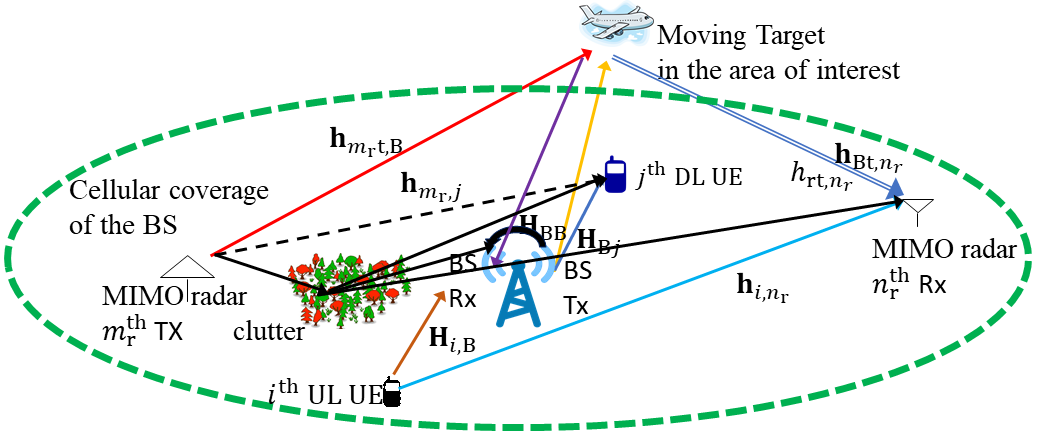
\includegraphics[width=1\columnwidth]{setup_model_tsp.png}
	%\vspace{-pt}
	\caption{Co-design system model comprising a statistical (widely distributed) MIMO radar and IBFD MU-MIMO communications.}
	\label{fig:setup}
	\vspace{-1em}
\end{figure}
Consider a statistical MIMO radar whose goal is to detect a moving target in a region that is coterminous with the cellular coverage of a BS which receives data from $\mathit{I}$ UL UEs while transmit it to $\mathit{J}$ DL UEs (Fig.~\ref{fig:setup}) %\textcolor{red}{Why is this in Roman numerals. It should also be Fig. 1}. 
The $M_\mathrm{r}$ Tx and $N_\mathrm{r}$ Rx of the statistical MIMO radar are located in a 2-D plane $\left(x,y \right)$ along with the BS, the $I$ UL UEs and the $J$ DL UEs at coordinates $\left(x_{m_\mathrm{r}},y_{m_\mathrm{r}}\right)$, $m_\mathrm{r}\in{Z}_{+}(M_\mathrm{r})$ and $\left(x_{n_\mathrm{r}},y_{n_\mathrm{r}} \right)$, $n_\mathrm{r}\in\mathbb{Z}_{+}(N_\mathrm{r})$, $(x_{\mathrm{B}},y_{\mathrm{B}})$, $(x_{n_i},y_{n_i})$, and $(x_{n_j},y_{n_j})$, $n\in\mathbb{Z}_{+}(N)$, respectively. In the sequel, we describe the system models of each of these units in detail and then present the co-design formulation.
\vspace{-1em}
\subsection{Statistical MIMO Radar System}
%which consists of a statistical MIMO radar composed of $M_\mathrm{r}$ transmitters (Tx) and $N_\mathrm{r}$ receivers (Rx), a communications BS equipped with $M_\mathrm{c}$ antennas and $\mathit{J}$ active user equipment (UEs), where each UE $\mathit{J}$ is equipped with $\mathit{N}^\textrm{d}_j$ transmit/receive antennas for all $j\in\mathbb{Z}_{+}(J)$. 
% \subsubsection{MIMO Radar Model}\label{mimoradarsys}
%The $M_\mathrm{r}$ Tx and $N_\mathrm{r}$ Rx of the MIMO radar as well as the BS and the $N$ UEs are located in a 2-D plane $\left(x,y \right)$ at coordinates $\left(x_{m_\mathrm{r}},y_{m_\mathrm{r}}\right)$, $m_\mathrm{r}\in{Z}_{+}(M_\mathrm{r})$ and $\left(x_{n_\mathrm{r}},y_{n_\mathrm{r}} \right)$, $n_\mathrm{r}\in\mathbb{Z}_{+}(N_\mathrm{r})$, as well as $(x_{\textrm{B}},y_{\textrm{B}})$ and $(x_{\mathrm{n}},y_{\mathrm{n}})$, $n\in\mathbb{Z}_{+}(N)$, respectively. 
 %The statistical MIMO radar is composed of $\mathit{M}_\textrm{r}$ single antenna Txs and $\mathit{N}_\mathrm{r}$ Rxs. 
Each radar Tx emits a pulse train of $\mathit{K}$ pulses at a pulse repetition interval (PRI) of $\mathit{T}_\textrm{r}$ toward targets-of-interest; this yields a \textit{coherent processing interval} (CPI) of $K\mathit{T}_\textrm{r}$. %The $\mathit{K}$ is chosen such that the range migration does not occur for the duration of the pulse train\cite{Xiaodong_Overlaid}. 
The pulse train corresponding to the $\ith{m\rr}$ Tx is modulated by the waveform code $\mathbf{a}_{m\rr}\in\mathbb{C}^{K}$ %\textcolor{red}{Should be $\mathbf{a}_{m_r}$? Or this is same for each Tx? Why its length depends on the number of Tx?}. 
and the MIMO radar code matrix is $\mathbf{A}=\bracket{\mathbf{a}^\top\bracket{1};\cdots; \mathbf{a}^\top\bracket{\mathrm{\mathit{K}}}}\in\mathbb{C}^{\mathit{K}\times \mathit{M}\rr}$, where $\mathbf{a}\bracket{k}=\bracket{a_{1}\bracket{k},\cdots,a_{\mathit{M}\rr}\bracket{k}}^\top$ is a radar code vector transmitted during the $\ith{k}$ PRI. Each pulse duration is $T_\mathit{P}= T_\mathrm{r}/N$, where $N\in\mathbb{Z}$ denotes the number of range cells/samples in a single PRI. The pulse train emitted by the $\ith{m_\mathrm{r}}$ Tx is\par\noindent\small
\begin{IEEEeqnarray}{rCl}
s_{m_\mathrm{r}}(t)=\sum_{k=1}^{\mathit{K}}a_{m_\mathrm{r},k}\phi_{m_\mathrm{r}}\paren{t-(k-1)T_\mathrm{r}},
\end{IEEEeqnarray}\normalsize
where $\phi_{m_\mathrm{r}}(t)$
%$\tau \in\left[0,T_\textrm{B} \right)$, $k\in \mathbb{Z}(K)$, and $l_\mathrm{s}\in \mathbb{Z}^+(L_\mathrm{s})$ denote the radar Tx antenna index, the fast time, i.e., the time index within one pulse, the slow time, i.e., the index of radar pulse, and the subpulse index, respectively,
denotes the $\ith{m_\mathrm{r}}$ element of the narrowband transmit waveform vector $\boldsymbol{\phi}(t)=\left[ \phi_1(t),\dots,\phi_{M_\mathrm{r}}(t)\right]^\top$ that satisfies the orthonormality condition $\int_{T_\mathit{P}}^{}\boldsymbol{\phi}(t)\boldsymbol{\phi}^\dagger(t)dt=\mathbf{I}_{M_\mathrm{r}}$.   The transmit signal of all Tx are $\mathbf{s}(t)=\bracket{s_1(t),\cdots,s_{M_\mathrm{r}}(t)}^\top$. 

%We first generalize the extended target model developed in the conventional MIMO radar research \cite{MIMOradarseparatedantennas,target_localization,widely_extendedtarget} to facilitate the co-design of MIMO radar and communications system. 
We consider a near-field scenario where the target scenario has an extended target composed of a large number of independent point-like scatterers. %In contrast to a far-field target, the distance and angle of a near-field target is a function of the transmit and receive element locations as well as the location of the individual scatterer\cite{fisher2006MIMO,haimovich2008mimo}. However, due to the central limit theorem and narrowband transmit signal assumption, 
The complex reflectivity of the extended target corresponding to the $\ith{m\rr}$ Tx - $\ith{n\rr}$ Rx link $h_{m\rr \target n\rr }$ is modeled as a CSCG random variable $h_{m\rr \target n\rr }\sim\mathcal{CN}(0,\eta^2_{m\rr\target n\rr})$, where $\eta^2_{m\rr\textrm{t}n\rr}$ denotes the average reflection power of the extended target; it remains constant over the CPI as per the Swerling I (block fading) target model \cite{fisher2006MIMO,haimovich2008mimo}. Collect the target reflectivities with respect to all Txs observed at the $\ith{n\rr}$ radar Rx in a vector $\mathbf{h}_{\textrm{rt,}n\rr}\triangleq\bracket{h_{1\textrm{t}n\rr},\cdots,h_{M\rr\textrm{t}n\rr}}^\top\in\mathbb{C}^{M\rr}$. 

%Furthermore, the waveforms $\braces{\boldsymbol{\phi}(t)}_{m\rr=1}^{\mathit{M}\rr}$ are narrowband. \cite{MIMOradarseparatedantennas,spacetimecodemimo,MCMIMO_Rad,target_localization}
%Assume that the coverage of this statistical MIMO radar has a moving target, which is characterized by ts complex reflectivity, location \textcolor{red}{all details related to the location also removed?}, and Doppler velocity \textcolor{red}{You have removed all the previous details that connected the velocity to frequency. Those details are needed.}. The complex reflectivity of the target with respect to the $\ith{m\rr}$ Tx - $\ith{n\rr}$ Rx pair is specified by a CSCG random variable $h_{m\rr \target n\rr }\sim\mathcal{CN}(0,\eta^2_{\target})$, where $\eta^2_{\target}$ \textcolor{red}{Why is this power not dependent on the specific Tx-Rx path chosen?} denotes the average reflection power of the target and is considered constant over the CPI \cite{sun2019target}. The Doppler frequency of the target with respect to the same $\ith{m\rr}$ Tx - $\ith{n\rr}$ Rx pair is $f^\prime_{m_\mathrm{r}\target n_\mathrm{r}}$ that we normalize by the PRI as $f_{m_\mathrm{r}\target n_\mathrm{r}}= f^\prime_{m_\mathrm{r}\target n_\mathrm{r}}\mathit{T}\rr$\cite{hongbin_movingtarget}. The motion of the target is slow enough such that $f'_{m_\mathrm{r}\target n_\mathrm{r}}$ remains constant within each pulse. %and fluctuates from pulse to pulse. 

%\textcolor{red}{No mention of analog signal, downconversion, sampling? These are very important details.} 
The velocity of the target is the vector  $\boldsymbol{\nu}_{\mathrm{t}}\triangleq\left(\nu_\mathrm{\mathrm{x},\mathrm{t}},\nu_\mathrm{\mathrm{y},\mathrm{t}} \right)$, where $\nu_\mathrm{\mathrm{x},\mathrm{t}}$ and $\nu_\mathrm{\mathrm{y},\mathrm{t}}$ are deterministic but unknown horizontal and vertical velocity components in the 2-D plane. The Doppler frequency with respect to the $\ith{m\rr}$ Tx - $\ith{n\rr}$ Rx pair is $f_{m_\mathrm{r}\target n_\mathrm{r}} = \frac{\nu_\mathrm{\mathrm{x},\mathrm{t}}}{\lambda}(\cos\theta_{m_\mathrm{r}\target}+\cos\phi_{n_\mathrm{r}\target})+\frac{\nu_\mathrm{\mathrm{y},\target}}{\lambda}(\sin\theta_{m_\mathrm{r}\target}+\sin\phi_{n_\mathrm{r}\target})$ \cite{hongbin_movingtarget},
\iffalse
\par\noindent\small
\begin{IEEEeqnarray}{rCl}
	%\begin{IEEEeqnarray}{rCl} 
	%\IEEEyesnumber\IEEEyessubnumber*
	f_{m_\mathrm{r}\target n_\mathrm{r}} &=& \frac{\nu_\mathrm{\mathrm{x},\mathrm{t}}}{\lambda}(\cos\theta_{m_\mathrm{r}\target}+\cos\phi_{n_\mathrm{r}\target})\nonumber\\
	&&+\frac{\nu_\mathrm{\mathrm{y},\target}}{\lambda}(\sin\theta_{m_\mathrm{r}\target}+\sin\phi_{n_\mathrm{r}\target}) \nonumber  \label{normalized doppler}
	%\end{IEEEeqnarray}
\end{IEEEeqnarray}\normalsize
\fi
where $\lambda$ denotes the carrier wavelength, $\theta_{m_\mathrm{r}}$ and $\phi_{n_\mathrm{r}}$ are the angles of departure at the $\ith{m_\mathrm{r}}$ Tx and angles of arrival at the $\ith{n_\mathrm{r}}$ Rx, respectively. %, with respect to the target. 
The narrowband assumption of $s_{m\rr}(t)$ allows us to approximate the propagation delay arising from the reflection off an arbitrary scatterer of the $\ith{n_\mathrm{r}}$ extended target to that from the center of gravity of the $\ith{n_\mathrm{r}}$ extended target, for all $m_\mathrm{r}\in\mathbb{Z}_{+}(M_\mathrm{r})$ and $n_\mathrm{r}\in\mathbb{Z}_{+}(N_\mathrm{r})$\cite{haimovich2008mimo}. If center of gravity of the extended target is $(x_{\mathrm{t}},y_{\mathrm{t}})$, then the the propagation delay with respect to $\ith{m\rr}$ Tx - $\ith{n\rr}$ Rx  is
$\zeta_{m\rr \target n\rr}=\frac{\sqrt{\paren{x_{m\rr}-x_{\mathrm{t}}}^2+\paren{y_{m\rr}-y_{\mathrm{t}}}^2}}{c}
		+\frac{\sqrt{\paren{x_{n\rr}-x_{\mathrm{t}}}^2+\paren{y_{n\rr}-y_{\mathrm{t}}}^2}}{c},$
\iffalse
\par\noindent\small
	\begin{IEEEeqnarray}{rCl}
		\zeta_{m\rr \target n\rr }&=&\frac{\sqrt{\paren{x_{m\rr}-x_{\mathrm{t}}}^2+\paren{y_{m\rr}-y_{\mathrm{t}}}^2}}{c}\nonumber\\
		&&+\frac{\sqrt{\paren{x_{n\rr}-x_{\mathrm{t}}}^2+\paren{y_{n\rr}-y_{\mathrm{t}}}^2}}{c}\nonumber
	\end{IEEEeqnarray} \normalsize
\fi
where $c=3\times 10^8$ m/s is the speed of the light. The slow-motion assumption of the target guarantees that $\zeta_{m\rr \target n\rr }$ is constant during each CPI. %, which further infers that the target remains in the same range cell over the entire CPI\cite{fisher2006MIMO}. 

The baseband signal at the $\ith{n\rr}$ Rx due to reflection off the target during the observation time $t\in[0,KT_r]$ is\par\noindent\small
\begin{align}
\label{target return_CT}
&y_{\mathrm{t},n\rr} (t)=\sum_{m_\mathrm{r}=1}^{M_\mathrm{r}}h_{m_\mathrm{r}\target n_\mathrm{r}}s_{m_\mathrm{r}}(t-\zeta_{m\rr \target n\rr }) \\
&\hspace{-4mm}\approx \sum_{m_\mathrm{r}=1}^{M_\mathrm{r}}\sum_{k=1}^{K} h_{m_\mathrm{r}\target n_\mathrm{r}}a_{m_\mathrm{r},k}\phi_{m_\mathrm{r}}\paren{t-\paren{k-1}T\rr-\zeta_{m\rr \target n\rr}}e^{j2\pi t
f_{m_\mathrm{r}\target n_\mathrm{r}}}, \label{approximation} 
\end{align}\normalsize
where $f'_{m_\mathrm{r}\target n_\mathrm{r}}\triangleq f_{m_\mathrm{r}\target n_\mathrm{r}}T\rr$ is the normalized Doppler frequency and the approximation in (\ref{approximation}) follows from the ``slow target'', i.e. $f'_{m_\mathrm{r}\target n_\mathrm{r}}$ %$f_{m_\mathrm{r}\target n_\mathrm{r}}T\rr$ 
is constant within a pulse \cite{hongbin_movingtarget,MCMIMO_Rad}.
Collect the exponential terms in a vector $\mathbf{q}_{\mathrm{r},n\rr}\bracket{k}=\bracket{e^{j2\pi\paren{k-1}f'_{1 \target n\rr}},\cdots,e^{j2\pi\paren{k-1}f'_{M\rr \target n\rr}}}^\top\in\mathbb{C}^{M\rr}$ and $\mathbf{Q}\rnr\bracket{k}=\diag\paren{\mathbf{q}_{\mathrm{r},n\rr}\bracket{k}}$.

The received signal $y_{\mathrm{r},n\rr}(t)$ is sampled at the rate $F_\textrm{c}=1/T_\textrm{c}$ to yield discrete-time samples $y_{\mathrm{r},n\rr}\bracket{n}$. These are then processed by a matched filter bank composed of $M\rr$ filters, where the $\ith{m\rr}$ filter is matched to the waveform $\phi_{m_\mathrm{r}}(t)$ %in order to extract the returns due to each MIMO radar transmit element 
\cite{MCMIMO_Rad}. The output of the matched filter peaks at the time instant that corresponds to the range location of the target; the range resolution is set by the pulse length $T_\mathit{P}$ \cite{richards2010principles}. Assuming that the range cells are aligned \cite{mishra2019cognitive} across all $N\rr$ Rx, the target is observed at the $\ith{n}$ range cell, where $n=\lfloor \sfrac{\zeta_{m\rr \target n\rr}}{T_\mathit{P}}\rfloor\in\mathbb{Z}_+\braces{N}$ %$n=1,\cdots,\lfloor \sfrac{\zeta_{m\rr \target n\rr}}{T_\mathit{P}}\rfloor$ for all $n\rr\in\mathbb{Z}_{+}\paren{N\rr}$ %\textcolor{red}{Is $\paren{N\rr} = \sfrac{\zeta_{m\rr \target n\rr}}{T_\mathit{P}}\rfloor$? Why do you change it to $L-1$ in Section II.C?}\textcolor{blue}{ $n\rr$ is for the subscript of $\zeta_{m\rr \target n\rr}$ } %\textcolor{red}{Ok. Fix it accordingly in both sections.}
\footnote{In general, the statistical MIMO radar receiver employs data association algorithms to ascertain the location and Doppler frequencies of each target using echoes from all Tx-Rx pairs. These algorithms are beyond the scope of this paper; we refer the reader to standard literature, e.g. \cite{Nayebi13dataassociation}, for details. %As a result, we https://www.overleaf.com/project/5c42348279d0c14d49731296do not target a specific MIMO radar array structure as shown in \cite{Nayebi13dataassociation}.
}. At the matched filter bank output for the $\ith{n\rr}$ Rx, denote the received signal samples from a target observed at the $\ith{n}$ range cell by a vector $\mathbf{y}_{\mathrm{t},n\rr,n}\in\mathbb{C}^{K}$ such that %a range cell under test (CUT) by the vector
%by $\mathbf{y}_{\mathrm{t},n\rr,n}$, whose $\ith{k}$ element is
\par\noindent\small 
\begin{align}\label{radar range cell}
	\mathbf{y}_{\mathrm{t},n\rr,n}\bracket{k}=\mathbf{h}^\top_{\mathrm{rt},n\rr}\mathbf{Q}_{\mathrm{r,}n\rr}\bracket{k}\mathbf{a}\bracket{k}\triangleq\mathbf{h}^\top_{\mathrm{rt},n\rr}\mathbf{s}_{\mathrm{rt,}n\rr}\bracket{k},\; k =1,\cdots,K.
\end{align}\normalsize
Note that we focus on the matched filter output at the $\ith{n}$ range cell, or cell under test (CUT), and therefore drop the cell index $n$ in the sequel.  Here, define $\mathbf{S}\rnr=\bracket{\mathbf{Q}\rnr\bracket{1}\mathbf{a}\bracket{1},\cdots,\mathbf{Q}\rnr\bracket{K}\mathbf{a}\bracket{K}}$. 
%\begin{IEEEeqnarray}{rCl}\label{radar range cell}
\iffalse
At the output of the matched filter of the $\ith{n\rr}$ Rx, denote the received signal samples from a target observed at a range cell under test (CUT) by the vector $\mathbf{y}_{\target,n\rr}=\bracket{y_{\mathrm{t},n\rr}\paren{1},\cdots,y_{\mathrm{t},n\rr}\paren{\mathit{K}}}^\top\in\mathbb{C}^{\mathit{K}}$, where $y_{\target,n\rr}\bracket{k}$ is \cite{NaghshTSP2017} \par\noindent\small
\begin{IEEEeqnarray}{rCl}\label{radar range cell}
y_{\mathrm{t},n\rr}\bracket{k}=\mathbf{h}^\top_{\mathrm{rt},n\rr}\mathbf{Q}_{\mathrm{r,}n\rr}\bracket{k}\mathbf{a}\bracket{k},
\end{IEEEeqnarray}\normalsize
where $\mathbf{Q}\rnr\bracket{k}=\diag\paren{\bracket{e^{j2\pi\paren{k-1}f'_{1 \target n\rr}},\cdots,e^{j2\pi\paren{k-1}f'_{\mathit{M}\rr \target n\rr}}}^\top}$.
\fi
%and $\mathbf{q}_{\mathrm{r},n\rr}\bracket{k}\triangleq\bracket{e^{j2\pi\paren{k-1}f'_{1 \target n\rr}},\cdots,e^{j2\pi\paren{k-1}f'_{\mathit{M}\rr \target n\rr}}}^\top\in\mathbb{C}^{\mathit{M}\rr}$
%We further define the temporal steering matrix from the $\mathit{M}\rr$ Txs to the $\ith{n\rr}$ Rx as $\mathbf{Q}_{\mathrm{r},n\rr}\triangleq\bracket{\mathbf{q}_{1 \target n\rr},\cdots,\mathbf{q}_{\mathit{M}\rr \target n\rr}}\in\mathbb{C}^{K\times \mathit{M}\rr}$, where the $\ith{m\rr}$ column $\mathbf{q}_{m\rr \target n\rr}=\bracket{1,\cdots,e^{j2\pi\paren{K-1}f'_{m\rr \target n\rr}}}^\top$. 
\iffalse
Next, $y_{\mathrm{r},n\rr}(t)$ is processed by a matched filter bank composed of $\mathit{M}\rr$ filters, where the $\ith{m\rr}$ filter is matched to the waveform $\phi_{m_\mathrm{r}}(t)$ in order to extract the returns due to each MIMO radar transmit element \cite{Vaidyanathan_MIMO_Waveform,MCMIMO_Rad}. The range resolution is set by the pulse length $T_\mathit{P}$ and each range cell is determined by the peak output of the matched filter through which the received echo signal is passed \cite{richards2010principles}. We also assume the cell synchronization is achieved across the $\mathit{N}\rr$ MIMO radar Rxs and the target is observed at the $\ith{n}$ range cell, i.e., $\lfloor \sfrac{\zeta_{m\rr \target n\rr}}{T_\mathit{P}}\rfloor=n$ for all $n\rr\in\mathbb{Z}_{+}\paren{\mathit{N}\rr}$. Denoting the matched filter bank output due to the target return at the $\ith{n\rr}$ MIMO radar Rx by $\mathbf{y}_{\mathrm{t},n\rr,n}$, whose $\ith{k}$ element is\par\noindent\small 
\begin{IEEEeqnarray}{rCl}\label{radar range cell}
\mathbf{y}_{\mathrm{t},n\rr,n}\bracket{k}=\mathbf{h}^\top_{\mathrm{rt},n\rr}\mathbf{Q}_{\mathrm{r,}n\rr}\bracket{k}\mathbf{a}\bracket{k}\triangleq\mathbf{h}^\top_{\mathrm{rt},n\rr}\mathbf{s}_{\mathrm{rt,}n\rr}\bracket{k}
\end{IEEEeqnarray}\normalsize
\fi
%$\mathbf{s}_{\textrm{rt},n\rr}=\bracket{\mathbf{Q}\rnr\bracket{1}\mathbf{a}\bracket{1},\cdots,\mathbf{Q}\rnr\bracket{\mathrm{\mathit{K}}}\mathbf{a}\bracket{\mathrm{\mathit{K}}}}$. 

In practice, apart from the target, the radar also receives echoes from undesired targets or clutter such as buildings and forests. % \cite{Xiaodong_Overlaid,d2020uplink} that the communications UEs are particularly vulnerable to the undesired reflections or reverberations produced by clutter, we herein utilize the clutter model documented in \cite{NaghshTSP2017}, where 
The clutter echoes are treated as signal-dependent interference produced by many independent and unambiguous point-like scatterers \cite{NaghshTSP2017}. Denote the clutter trail at the CUT of $\ith{n\rr}$ Rx by a $K \times 1$ vector $\mathbf{y}_{\mathrm{c},n\rr}$ whose covariance matrix (CM) is $\mathbf{R}_{\textrm{c},n\rr}\in\mathbb{C}^{\mathit{K}\times K}$%\textcolor{red}{How auto-covariance matrix is rectangular?}
, with its $\ith{\paren{m,\ell}}$ element being $\mathbf{R}_{\textrm{c},n\rr}\paren{m,\ell}=\sigma^2_{\textrm{c},n\rr}\rho_{\mathrm{c}}^{\lvert m-\ell\rvert}$,
%We consider an exponential correlation shape for $\mathbf{R}_{\textrm{c},n\rr}$, 
\iffalse
\par\noindent\small 
\begin{IEEEeqnarray}{rCl}\label{clutter cov}
\mathbf{R}_{\textrm{c},n\rr}\bracket{m,\ell}=\sigma^2_{\textrm{c},n\rr}\rho^{\lvert m-\ell\rvert}
\end{IEEEeqnarray}\normalsize
\fi
where $\sigma^2_{\textrm{c},n\rr}$ is the clutter power observed by $\ith{n\rr}$ Rx and $\rho$ is a constant \cite{NaghshTSP2017}. 
\vspace{-1em}
\subsection{IBFD MU-MIMO Communications}
Consider a FD BS equipped with $\mathit{M}_\textrm{c}$ transmit and $\mathit{N}_{\textrm{c}}$ receive antennas. There are a total of $\mathit{I}$ UL ($\mathit{J}$ DL) UEs, which function in HD mode simultaneously uploading (downloading) packets during a predefined \textit{scheduling  window}. Every $\ith{i}$ UL ($\ith{j}$ DL) UE employs $\mathit{N}^{\textrm{u}}_i$ ($\mathit{N}^{\textrm{d}}_j$) transmit-receive antennas. % for all $\braces{i}$ and $\braces{j}$ %$j\in\mathbb{Z}_{+}(\mathit{J})$. 
To achieve the maximum capacity of the UL channels, assume $\mathit{M}\cc\geq\sum_{i=1}^{\mathit{I}}\mathit{N}^{\textrm{u}}_i$\cite{tse2005fundamentals}. To facilitate the co-design, the length of the scheduling window is same as the radar CPI; hence, the CPI should exceed the maximum latency required by the UL or DL transmissions \cite{ShiftMIMO}. Further, the length of a UL/DL frame is identical to the PRI and the duration of UL/DL symbols is same as that of the radar pulses. It follows that the number of the frames transmitted in a given window is $\mathit{K}$ and the number of the symbols sent in each frame is $\mathit{N}$. %For the simplicity of analysis, 
In this context, the MIMO radar and IBFD MU-MIMO communications systems are fully synchronous \cite{MCMIMO_RadComm}. 

Denote the number of data streams as $\mathrm{D}^\textrm{u}_i\leq \mathit{N}^{\textrm{u}}_i$. During the $\ith{l}$ symbol period of the $\ith{k}$ frame, the $\ith{i}$ UL UE sends a unit-energy symbol vector $\mathbf{d}_{\textrm{u},i}\bracket{k,l}\in \mathbb{C}^{D^{\textrm{u}}_i}$ to the BS, where $\mathbf{d}_{\textrm{u},i}\bracket{k,l}$ is independent and identically distributed (i.i.d.) for $i\in\mathbb{Z}_+\braces{\mathit{I}}$, $k\in\mathbb{Z}_+\braces{\mathit{K}}$, and $l\in\mathbb{Z}_+\braces{\mathit{N}}$. 
The precoder of $\ith{i}$ UL UE for the $\ith{k}$ frame is the matrix $\PiB\in\mathbb{C}^{\mathit{N}^{\textrm{u}}_i\times \mathit{D}^\textrm{u}_i}$ so that the discrete-time transmit signal at this UE is $\mathbf{s}_{\textrm{u},i}\bracket{k,l}=\PiB\mathbf{d}_{\textrm{u},i}\bracket{k,l}$. The UL from the $\ith{i}$ UL UE to the BS is a multiple access channel (MAC) $\mathbf{H}_{i,\textrm{B}}\in\mathbb{C}^{\mathit{M}\cc\times \mathit{N}^{\textrm{u}}_i}$. The analog received signal is processed through conventional stages such as downconversion, symbol rate sampling, matched filtering, and time/frequency synchronization. The resulting discrete-time received signal at the BS from the $\ith{i}$ UL UE is\cite{Heathvehicularcommradar} \par\noindent\small
%\begin{IEEEeqnarray}{rCl} 
\begin{equation}
\label{eq:ULFDcomm}
%\mathbf{y}_{i,\textrm{B}}\bracket{k,l}=\mathbf{H}_{i,\textrm{B}}\PiB\dui.
\mathbf{y}_{i,\textrm{B}}\bracket{k,l}=\mathbf{H}_{i,\textrm{B}}\mathbf{s}_{\textrm{u},i}\bracket{k,l}.
%\mathbf{y}_{i,\B}\bracket{k,l}=\sum_{i=1}^I\mathbf{H}_{i,\textrm{B}}\PiB\dui
%\end{IEEEeqnarray}
\end{equation}\normalsize
At the $\ith{i}$ UL UE, the simultaneous transmissions of the rest of UL UEs lead to the multi-user interference (MUI)\footnote{The MU transmission here is via linear precoders which have lower complexity than the optimal dirty paper coding \cite{tse2005fundamentals}.}  \par\noindent\small
\begin{align}
\mathbf{y}_{\textrm{um},i}\bracket{k,l}=\sum_{q\neq i}\mathbf{H}_{q,\textrm{B}}\mathbf{s}_{\textrm{u},q}\bracket{k,l}.\label{eq:mui}
\end{align}\normalsize
The CMs of 
$\mathbf{y}_{i,\textrm{B}}\bracket{k,l}$ and $\mathbf{y}_{\textrm{um},i}\bracket{k,l}$ are  $\mathbf{R}_{\textrm{u},i}\bracket{k,l}=\HiB\PiB\PiBH\HiBH$ and
$\mathbf{R}_{\textrm{um},i}\bracket{k,l}=\sum_{g\neq i }\mathbf{H}_{g,\textrm{B}}\mathbf{P}_{\textrm{u},g}\mathbf{P}_{\textrm{u},g}\mathbf{H}^\dagger_{g,\textrm{B}}$, respectively.

At the DL, the $\mathit{J}$ UEs simultaneously download packets from the BS. During the $\ith{l}$ symbol period of the $\ith{k}$ frame, the symbol vector intended for the $\ith{j}$ DL UE is $\mathbf{d}_{\textrm{d},j}\bracket{k,l}\in \mathbb{C}^{\mathrm{D}^\textrm{d}_j}$, i.i.d in $k$ and $l$, where $\mathrm{D}^\textrm{d}_j\leq \min\paren{\mathit{M}\cc,\mathit{N}^{\textrm{d}}_j}$ denotes the number of unit-energy data streams. %$\mathbf{d}_{\textrm{B},j}\bracket{k,l}$ is also unit-energy, i.e., $\mathbb{E}\bracket{\mathbf{d}_{\textrm{B},j}\bracket{k,l}\mathbf{d}^\dagger_{\textrm{B},j}\bracket{k,l}}=\mathbf{I}_{\mathrm{D}^\textrm{d}_j}$ \cite{Gasussianduality}. %A complex precoding matrix is assigned to each UE to achieve multiple-access interference suppression and spatial diversity exploitation\cite{ArraytoMIMO,ShiftMIMO}. 
Given the precoding matrix for the $\ith{j}$ DL UE at the $\ith{k}$ frame as $\PBj\in\mathbb{C}^{\mathit{M}\cc\times \mathrm{D}^\textrm{d}_j}$, the signal vector transmitted from the BS to the $\ith{j}$ DL UE is $\mathbf{s}_{\textrm{d},j}\bracket{k,l}=\PBj\mathbf{d}_{\textrm{\textrm{d}},j}\bracket{k,l}$. The channel between the BS and the $\ith{j}$ DL UE is a broadcast (BC) channel $\mathbf{H}_{\textrm{B},j}\in\mathbb{C}^{\mathit{N}^\textrm{d}_j\times \mathit{M}\cc}$. The $\mathbf{H}_{\textrm{B},j}$ is full rank for all $j$ to achieve the highest spatial degrees of freedom of the MIMO-BC channel \cite{tse2005fundamentals}. After similar conventional processing as in the BS above, the resulting discrete-time DL signal at the $\ith{j}$ DL UE is\cite{Heathvehicularcommradar} \par\noindent\small
\begin{flalign}
\label{eq:DL1}
&\mathbf{y}_{\textrm{B},j}\bracket{k,l}=\mathbf{H}_{\textrm{B},j}\mathbf{s}_{\textrm{d},j}\bracket{k,l}+\mathbf{y}_{\textrm{dm},j}\bracket{k,l},
\end{flalign}\normalsize
where $\mathbf{y}_{\textrm{dm},j}\bracket{k,l}=\mathbf{H}_{\textrm{B},j}\sum_{g\neq j}^{}\mathbf{s}_{\textrm{d},g}\bracket{k,l}$
denotes the MUI of the $\ith{j}$ DL UE. Using the fact that the symbol vectors are i.i.d., the CMs of $\mathbf{y}_{\textrm{B},j}\bracket{k,l}$ and $\mathbf{y}_{\textrm{dm},j}\bracket{k,l}$ are $\mathbf{R}_{\textrm{dm},j}\bracket{k,l}=\sum_{g\neq j}\mathbf{H}_{\textrm{B},j}\PBg\mathbf{P}^{\dagger}_{\textrm{B},g}\bracket{k}\mathbf{H}^\dagger_{\textrm{B},j}$ and $\mathbf{R}_{\B,j}\bracket{k,l}=\mathbf{R}_{\textrm{dm},j}\bracket{k,l}+ \mathbf{H}_{\textrm{B},j}\PBj\PBjH\mathbf{H}^\dagger_{\textrm{B},j}$, respectively.

The FD transmission of the BS implies that its Rx is overlaid with the DL signals which are transmitted over the self-interference channel $\mathbf{H}_{\mathrm{BB}}\in{\mathbb{C}^{\mathit{N}\cc\times \mathit{M}\cc}}$. The self-interfering signal at the BS Rx is\par\noindent\small \begin{align}
\mathbf{y}_{\mathrm{BB}}\bracket{k,l}=\mathbf{H}_{\mathrm{BB}}\sum_{j=1}^{\mathit{J}}\PBj\mathbf{d}_{\textrm{B},j}\bracket{k,l}. \label{eq:sic}
\end{align}\normalsize
In the simultaneous UL-DL transmissions, the channel from $\ith{i}$ UL UE to $\ith{j}$ DL UE is $\mathbf{H}_{i,j}\in\mathbb{C}^{\mathit{N}^{\textrm{d}}_j\times \mathit{N}^{\textrm{u}}_i}$, with the CM $\mathbf{R}_{\mathrm{BB}}\bracket{k,l}=\sum_{j=1}^{\mathit{J}}\mathbf{H}_{\mathrm{BB}}\PBj\PBjH\mathbf{H}^\dagger_\mathrm{BB}$.
%for $i\in\mathbb{Z}^+\braces{\mathit{I}}$ and $j\in\mathbb{Z}^+\braces{\mathit{J}}$
Hence, the UL signal received at the $\ith{j}$ DL UE during the $\ith{l}$ symbol period of the $\ith{k}$ frame is\par\noindent\small
\begin{align}
\mathbf{y}_{\mathrm{u},j}\bracket{k,l}=\sum_{i=1}^{\mathit{I}}\mathbf{H}_{i,j}\PiB\dui,\label{eq:UL2}
\end{align}\normalsize
with the CM $\mathbf{R}_{\mathrm{u},j}\bracket{k,l}=\sum_{i=1}^{\mathit{I}}\mathbf{H}_{i,j}\PiB\PiBH\mathbf{H}^\dagger_{i,j}$. Assume perfect CSI at the Tx and Rx (CSITR) is available to the IBFD MU-MIMO communications as well as radar. The elements of $\mathbf{H}_{\textrm{B},j}$, $\mathbf{H}_{i,\textrm{B}}$, $\mathbf{H}_{i,j}$, and $\mathbf{H}_{\textrm{B,B}}$ are distributed as $\mathcal{CN}\paren{0,\eta^2_{\textrm{d},j}}$, $\mathcal{CN}\paren{0,\eta^2_{\textrm{u},i}}$, $\mathcal{CN}\paren{0,\eta^2_{i,j}}$, and $\mathcal{CN}\paren{0,\eta^2_{\textrm{BB}}}$, respectively, for all $i$ and $j$.
\iffalse
\par\noindent\small
\begin{flalign}
\mathbf{y}_{\mathrm{u},j}\bracket{k,l}=\sum_{i=1}^{\mathit{I}}\mathbf{H}_{i,j}\PiB\dui,
\end{flalign}\normalsize
\fi
\iffalse
Before proceeding, we define the CMs of $\mathbf{y}_{\textrm{u},i}\bracket{k,l}$, $\mathbf{y}_{\textrm{um},i}\bracket{k,l}$, $\mathbf{y}_{\mathrm{BB}}\bracket{k,l}$, $\mathbf{y}_{\textrm{dm},j}\bracket{k,l}$, $\mathbf{y}_{\textrm{B},j}\bracket{k,l}$ and $\mathbf{y}_{\textrm{UL},j}\bracket{k,l}$ as 
\par\noindent\small
\begin{flalign}
\mathbf{R}_{\textrm{u},i}\bracket{k,l}&=\HiB\PiB\PiBH\HiBH,\nonumber\\
\mathbf{R}_{\textrm{um},i}\bracket{k,l}&=\sum_{g\neq i }\mathbf{H}_{g,\textrm{B}}\PBg\PBgH\mathbf{H}^\dagger_{g,\textrm{B}},\nonumber\\
\mathbf{R}_{\mathrm{BB}}\bracket{k,l}&=\sum_{j=1}^{\mathit{J}}\mathbf{H}_{\mathrm{BB}}\PBj\PBjH\mathbf{H}^\dagger_\mathrm{BB}\nonumber\\
\mathbf{R}_{\textrm{dm},j}\bracket{k,l}&=\sum_{g\neq j}\mathbf{H}_{\textrm{B},j}\PBg\mathbf{P}^{\dagger}_{\textrm{B},g}\bracket{k}\mathbf{H}^\dagger_{\textrm{B},j}\nonumber\\
\mathbf{R}_{\B,j}\bracket{k,l}&=\mathbf{R}_{\textrm{dm},j}\bracket{k,l}+ \mathbf{H}_{\textrm{B},j}\PBj\PBjH\mathbf{H}^\dagger_{\textrm{B},j}\nonumber\\
\mathbf{R}_{\mathrm{u},j}\bracket{k,l}&=\sum_{i=1}^{\mathit{I}}\mathbf{H}_{i,j}\PiB\PiBH\mathbf{H}^\dagger_{i,j}
\end{flalign}\normalsize
%\fi
%\iffalse
$\mathbf{R}_{\textrm{u},i}\bracket{k,l}=$ $\HiB\PiB\PiBH\HiBH$,  $\mathbf{R}_{\textrm{um},i}\bracket{k,l}=$ $\sum_{g\neq i }\mathbf{H}_{g,\textrm{B}}\PBg\PBgH\mathbf{H}^\dagger_{g,\textrm{B}}$, $\mathbf{R}_{\mathrm{BB}}\bracket{k,l}=$ $\sum_{j=1}^{\mathit{J}}\mathbf{H}_{\mathrm{BB}}\PBj\PBjH\mathbf{H}^\dagger_\mathrm{BB}$, $\mathbf{R}_{\textrm{dm},j}\bracket{k,l}=$ $\sum_{g\neq j}\mathbf{H}_{\textrm{B},j}\PBg\mathbf{P}^{\dagger}_{\textrm{B},g}\bracket{k}\mathbf{H}^\dagger_{\textrm{B},j}$, $\mathbf{R}_{\B,j}\bracket{k,l}=\mathbf{R}_{\textrm{dm},j}\bracket{k,l}+$ $\mathbf{H}_{\textrm{B},j}\PBj\PBjH\mathbf{H}^\dagger_{\textrm{B},j}$, and $\mathbf{R}_{\mathrm{u},j}\bracket{k,l}=\sum_{i=1}^{\mathit{I}}\mathbf{H}_{i,j}\PiB\PiBH\mathbf{H}^\dagger_{i,j}$, respectively. 
\fi
\vspace{-1em}
\subsection{Joint Radar-Communications}
\label{Coexistence}
In joint radar-communications, the radar Rx signal is overlaid with the IBFD MU-MIMO communications signals leading to additional challenges in target detection. Similarly, the radar probing signals adversely impact the UL/DL rates. We now define the overlaid signals at the MIMO radar Rx (with contributions from the target, clutter, UL, direct DL, indirect DL, and noise) and BS (see Fig.~\ref{fig:systemmodel}). %Figure~\ref{fig:systemmodel} shows an overlaid signal diagram for the coexistence model where

%the $n\in\mathbb{Z}_+\braces{\mathit{L}-1}$ \textcolor{red}{Is $L-1 = \sfrac{\zeta_{m\rr \target n\rr}}{T_\mathit{P}}\rfloor$?} denotes the index for the CUT \textcolor{red}{No need to redefine CUT index. You already did that using different symbol notation in Section II.A}. 
 
The DL signal $\mathbf{s}_{\textrm{d},j}\bracket{k,l}$ is received at the $\ith{n\rr}$ radar Rx through a multi-path fading channel $\mathbf{h}_{\mathrm{Bm},n\rr}\in\mathbb{C}^{\mathit{M}_\mathrm{c}}\sim \mathcal{CN}\paren{0,\eta^2_{\textrm{Bm},n\rr}\mathbf{I}_{\mathit{M}_\mathrm{c}}}$ over a CPI. Assume that the time delay between the BS and each radar Rx is negligible. The DL signal at $\ith{n\rr}$ radar Rx in $
\ith{k}$ PRI is\par\noindent\small
\begin{equation}
y_{\mathrm{Bm},n\rr}\bracket{k}=\mathbf{h}_{\mathrm{Bm},n\rr}^\top e^{j2\pi\paren{k-1} f_{\mathrm{Bm}n_\mathrm{r}}}
\sum_{j=1}^\mathit{J}\mathbf{s}_{\textrm{d},j}\bracket{k,n+1},\label{eq:DL_direct}
\end{equation}\normalsize
%$y_{\mathrm{Bm},n\rr}\bracket{k}=\mathbf{h}_{\mathrm{Bm},n\rr}^\top e^{j2\pi\paren{k-1} f_{\mathrm{Bm}n_\mathrm{r}}}\sum_{j=1}^\mathit{J}\mathbf{s}_{\textrm{d},j}\bracket{k}$, 
where $f_{\mathrm{Bm}n_\mathrm{r}}$ denotes the normalized channel Doppler frequency.  

When a target is present, the $\ith{n\rr}$ radar Rx also receives the echoes of the DL signals reflected off the target through a reflection channel $\mathbf{h}_{\textrm{Bt,}n\rr}\sim\mathcal{CN}\paren{0,\eta^2_{\textrm{Bt},n\rr}\mathbf{I}}$. Throughout this paper, we assume that $\eta^2_{\textrm{rt},n\rr}$ and $\eta^2_{\textrm{Bt},n\rr}$ are perfectly known to the BS, all UEs and MIMO radar Rxs. Without loss of generality, consider a fully synchronous scenario, wherein $\mathbf{s}_{\textrm{d},j}\bracket{k}$ is reflected off the target before received by %arriving at the CUT of 
the $\ith{n\rr}$ radar Rx in each PRI over the channel $\mathbf{h}_{\textrm{Bt,}n\rr}$.
Denote the target's normalized Doppler frequency by $f_{\textrm{Bt,}n\rr}$. 
\iffalse
their corresponding temporal steering vectors can be written as $\mathbf{q}_{\mathrm{Bm},n\rr}=\bracket{1,\cdots,e^{j2\pi\paren{\mathit{K}-1} f_{\mathrm{Bm}n_\mathrm{r}}}}^\top$ and $\mathbf{q}_{\mathrm{Bt},n\rr}=\bracket{1,\cdots,e^{j2\pi\mathrm{\paren{K-1}}f_{\mathrm{Bt}n_\mathrm{r}}}}^\top$, respectively. 
\fi
The target echo from reflected DL signal at CUT of $\ith{n\rr}$ radar Rx during $\ith{k}$ PRI is\par\noindent\small
\begin{equation}
y_{\mathrm{Bt},n\rr}\bracket{k}=\mathbf{h}_{\mathrm{Bt},n\rr}^\top e^{j2\pi\paren{k-1} f_{\mathrm{Bt}n_\mathrm{r}}}
\sum_{j=1}^\mathit{J}\mathbf{s}_{\textrm{d},j}\bracket{k,1}.
\end{equation}\normalsize
%$\mathbf{S}_{\mathrm{Bm},n\rr}\triangleq$ $\bracket{\mathbf{s}^\top_{\mathrm{Bm},n\rr}\bracket{1};\cdots;\mathbf{s}^\top_{\mathrm{Bm},n\rr}\bracket{\mathrm{\mathit{K}}}}$, $\mathbf{s}_{\mathrm{Bm},n\rr}\bracket{k}=\mathbf{q}_{\mathrm{Bm},n\rr}\bracket{k}\sum_{j=1}^{\mathit{J}}\mathbf{s}_{\textrm{d},j}\bracket{k}$, $\mathbf{S}_{\mathrm{Bt,}n\rr}\triangleq$ $\bracket{\mathbf{s}^\top_{\mathrm{Bt},1}\bracket{1};\cdots;\mathbf{s}^\top_{\mathrm{Bt},n\rr}\bracket{\mathrm{\mathit{K}}}}$ and 
%,$\mathbf{q}_{\mathrm{Bm},n\rr}\bracket{k}=e^{j2\pi\paren{k-1}f_{\mathrm{Bm},n\rr}}$ and$\mathbf{q}_{\mathrm{Bt},n\rr}\bracket{k}=e^{j2\pi\paren{k-1}f_{\mathrm{Bt},n\rr}}$
%, $\mathbf{y}_{\target,n\rr}\triangleq\mathbf{S}_{\target,n\rr}\mathbf{h}_{\target,n\rr}$ and
\begin{figure}[!t]
	%\begin{figure*}[!t]
		\centering
		%	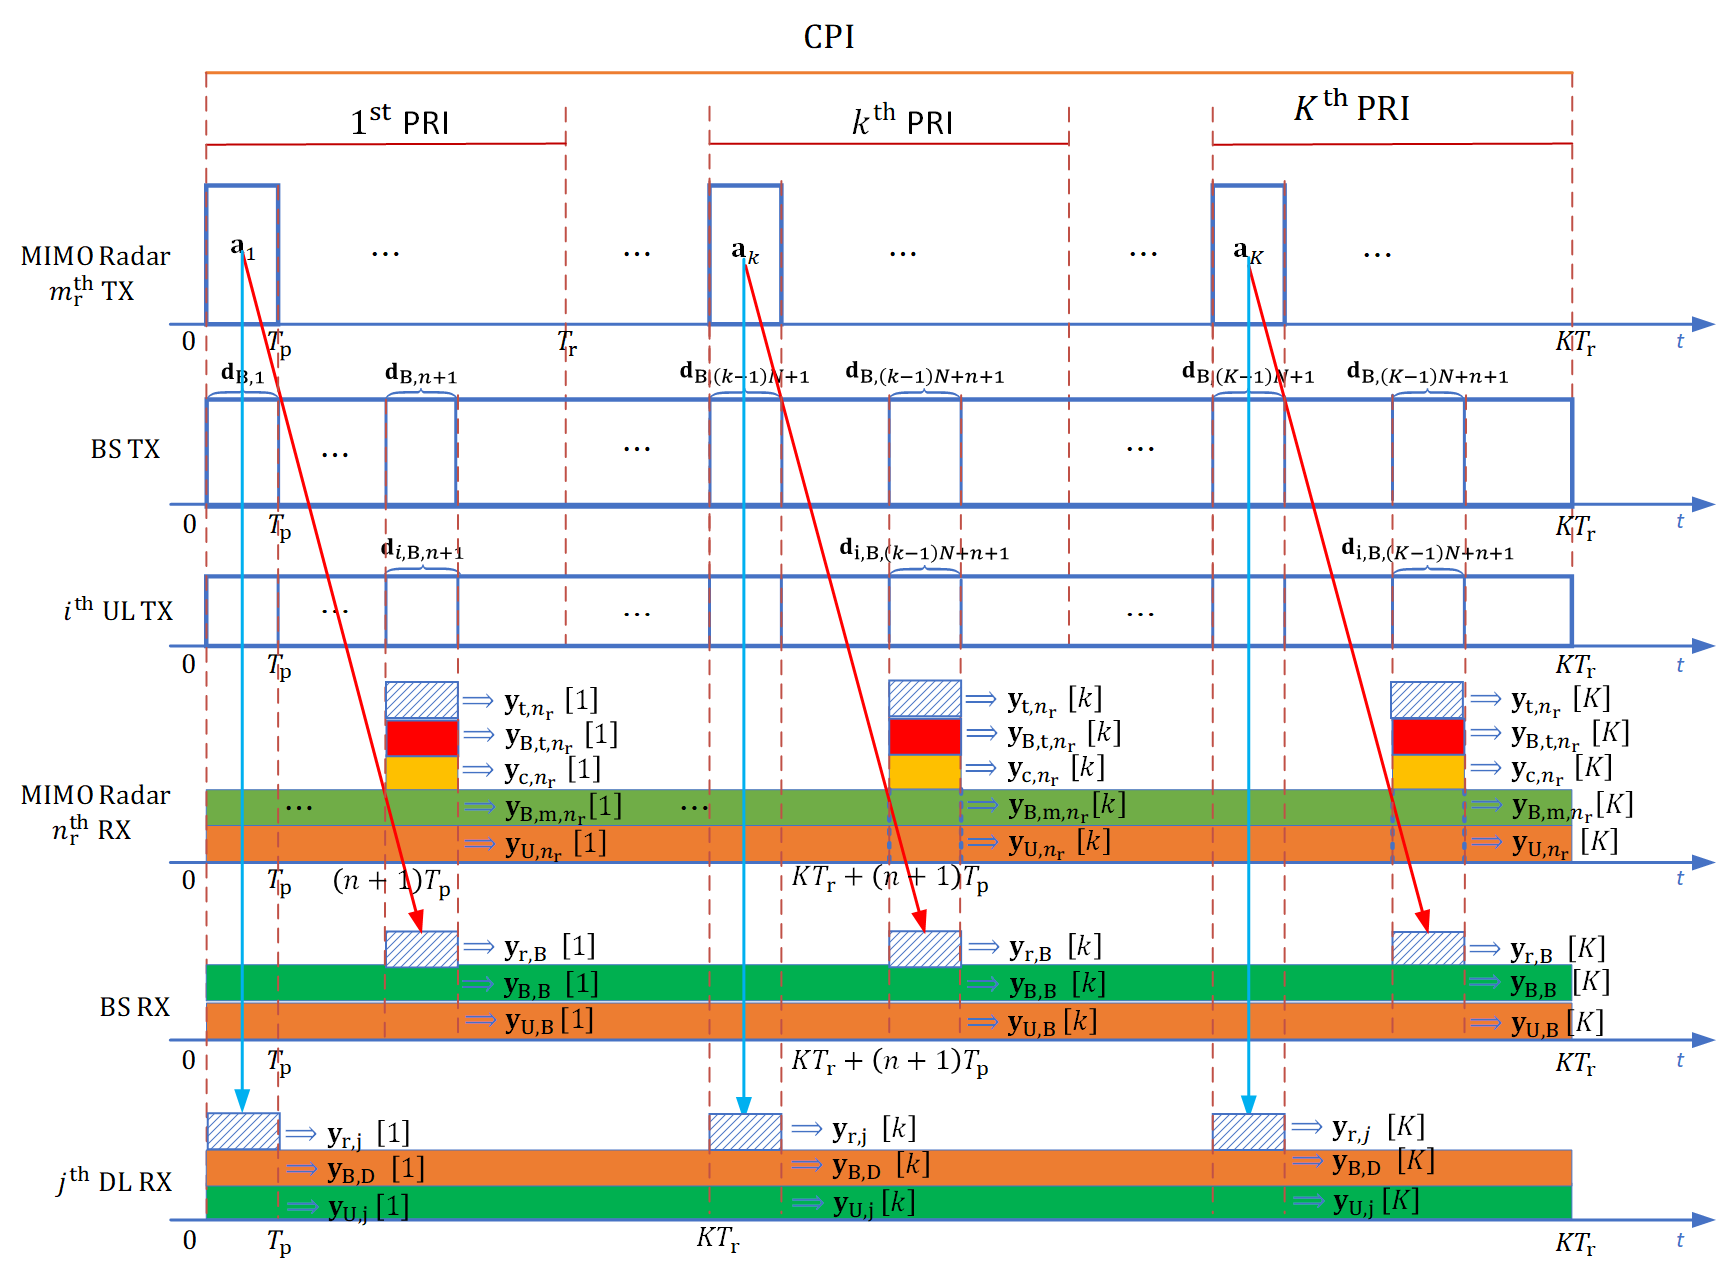
\includegraphics[width=3.1in]{Drawing3}
		%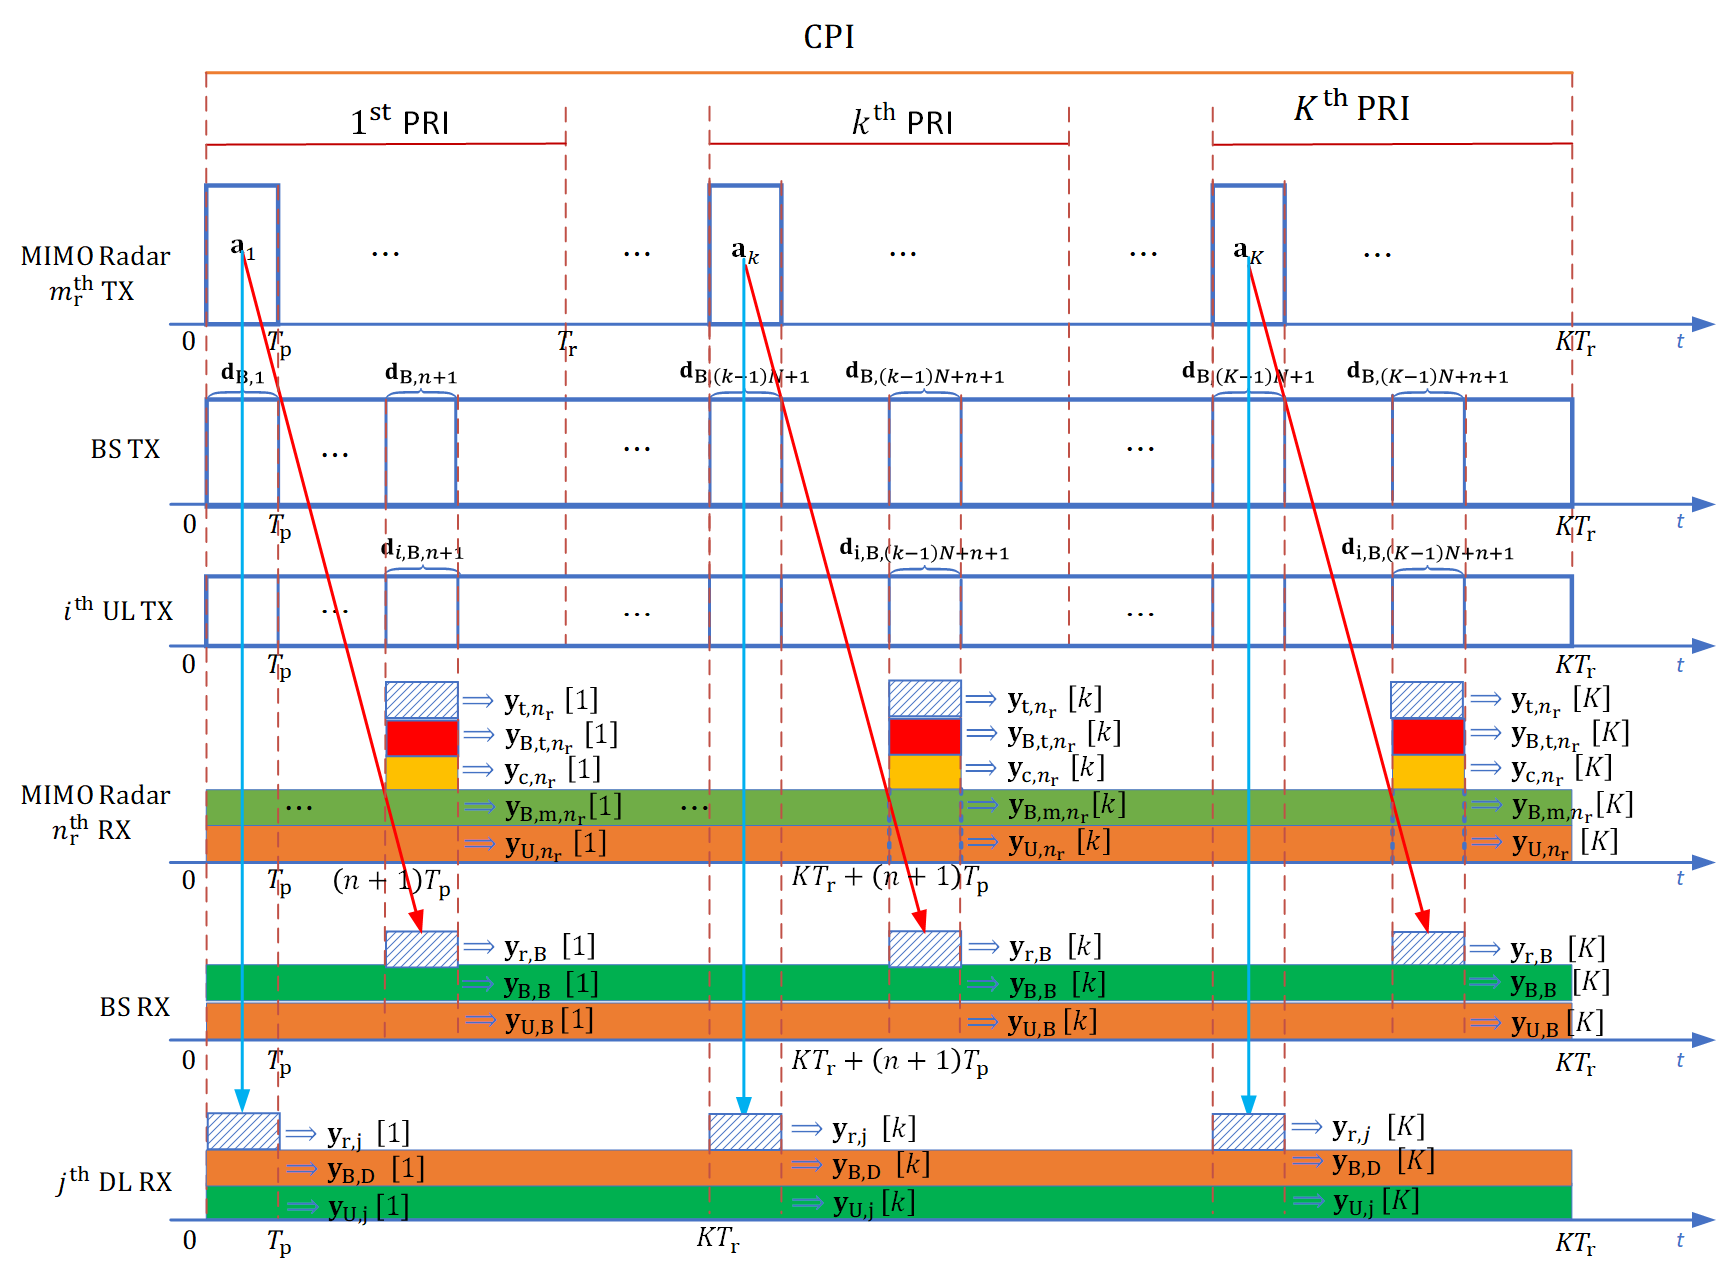
\includegraphics[width=0.80\textwidth]{Drawing3.png}
		%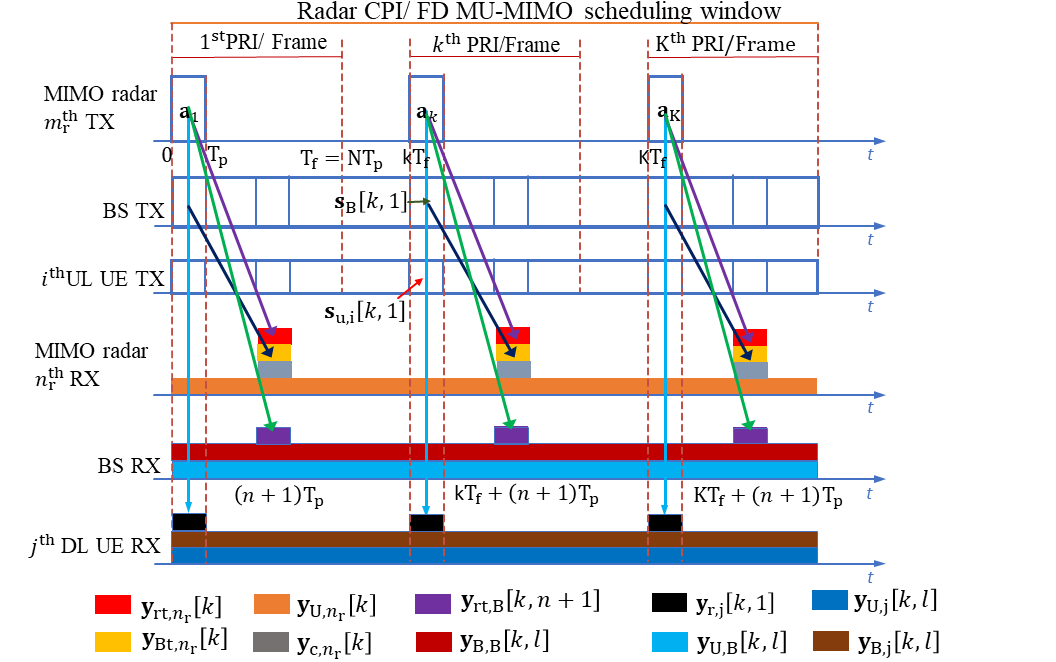
\includegraphics[width=0.80\textwidth]{systemmodel.png}
		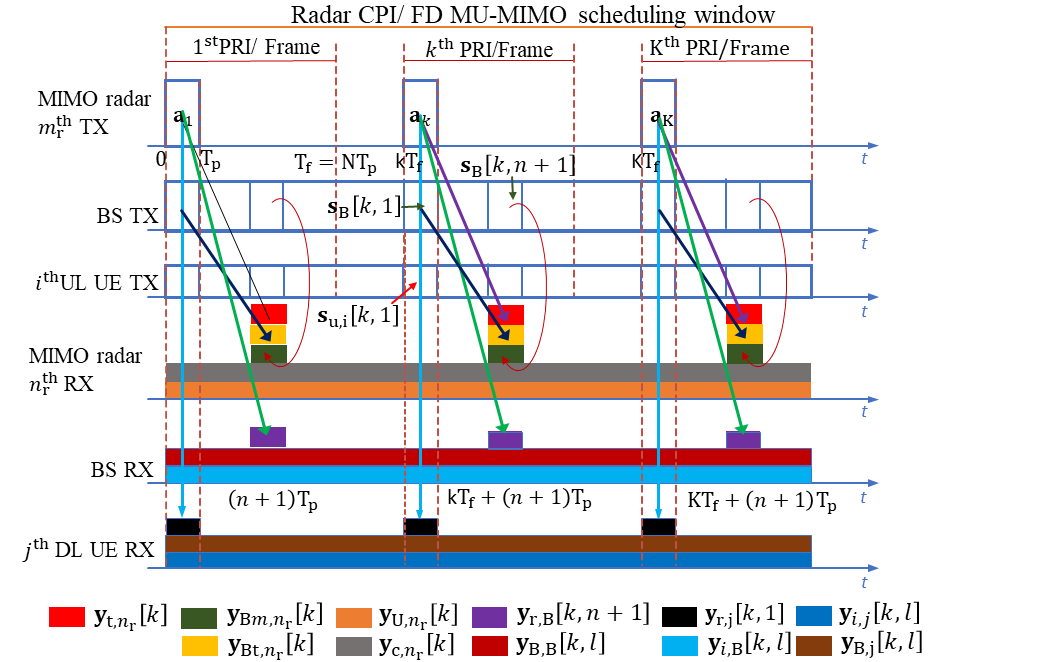
\includegraphics[width=1.0\columnwidth]{system_model_TSP.png}
		\caption{The overlaid signal timing diagram for one CPI is illustrated where the unit time scale is the pulse or symbol duration. For each MIMO radar Rx, we focus on the $\ith{n}$ range cell where the target is observed. The $\ith{j}$ UE is interfered by the radar probing signal during the symbol period when the MIMO radar transmits pulses. %\textcolor{red}{\textbf{The top text is cut off.}}
		} 
		\vspace{-2em}
		\label{fig:systemmodel}
	\end{figure} %Recall our discussion prior to (\ref{radar range cell}) that our radar system design will be focused on the components in the cell of interest. s

 Note that the target information is embedded in only  $\mathbf{y}_{\textrm{Bt,}n\rr}$. Hence, the effective number of antennas to detect the target is $\mathit{M}=\mathit{M}\cc+\MM\rr$. The overall radar target channel matrix is $\mathbf{h}_{\target,n\rr}=\bracket{\mathbf{h}^\top_{\textrm{rt},n\rr},\mathbf{h}^\top_{\textrm{Bt},n\rr}}^\top\in\mathbb{C}^{\mathit{M}}$ whose CM is $\mathbb{E}\bracket{\mathbf{h}_{\target,n\rr}\mathbf{h}^\dagger_{\target,n\rr}}\triangleq\boldsymbol{\Sigma}_{\target,n\rr}=\eta^2_{\textrm{rt},n\rr}\mathbf{I}\oplus\eta^2_{\textrm{Bt},n\rr}\mathbf{I}$. Denote $\mathbf{s}_{\mathrm{rt,}n\rr}\bracket{k}=\mathbf{Q}_{\mathrm{r,}n\rr}\bracket{k}\mathbf{a}\bracket{k}$ and $\mathbf{s}_{\mathrm{Bt},n\rr}\bracket{k}=e^{j2\pi\paren{k-1} f_{\mathrm{Bt}n_\mathrm{r}}}
\sum_{j=1}^\mathit{J}\mathbf{s}_{\textrm{d},j}\bracket{k}$, and define $\stnrk=\bracket{\mathbf{s}^\top_{\textrm{rt},n\rr}\bracket{k},\mathbf{s}^\top_{\textrm{Bt},n\rr}\bracket{k}}^\top=\mathbf{J}_{\textrm{r}}\srtnrk+\mathbf{J}_{\textrm{B}}\sBtnrk$, where $\mathbf{J}_{\textrm{r}}=\bracket{\mathbf{I}_{\mathit{M}\rr\times \mathit{M}\rr};\mathbf{0}_{\mathit{M}\cc\times \mathit{M}\rr}}\in\mathbb{R}^{\mathbf{\mathit{M}\times \mathit{M}\rr}}$ and $\mathbf{J}_{\textrm{B}}=\bracket{\mathbf{0}_{\mathit{M}\rr\times \mathit{M}\cc};\mathbf{I}_{\mathit{M}\cc\times \mathit{M}\cc}}\in\mathbb{R}^{\mathbf{\mathit{M}\times \mathit{M}\cc}}$. Combining the echoes from the DL link and the radar Tx, the target signal becomes
\begin{equation}
y_{\target,n\rr}\bracket{k}\triangleq\mathbf{h}^\top_{\textrm{rt},n\rr}\mathbf{s}_{\textrm{rt},n\rr}\bracket{k}+\mathbf{h}^\top_{\textrm{Bt},n\rr}\mathbf{s}_{\textrm{Bt},n\rr}\bracket{k}.    \label{eq:target1}
\end{equation} 

For a given CPI, denote %the compact forms of $y_{\mathrm{Bm},n\rr}\bracket{k}$ and $y_{\mathrm{Bt},n\rr}\bracket{k}$ by
$\mathbf{y}_{\mathrm{Bm},n\rr}\triangleq\bracket{y_{\mathrm{Bm},n\rr}\paren{1},\cdots,y_{\mathrm{Bm},n\rr}\paren{\mathit{K}}}^\top$ and  $\mathbf{y}_{\mathrm{Bt},n\rr}\triangleq\bracket{y_{\mathrm{Bt},n\rr}\paren{1},\cdots,y_{\mathrm{Bt},n\rr}\paren{\mathit{K}}}^\top$. The CMs of $\mathbf{y}_{\mathrm{Bm},n\rr}$ and $\mathbf{y}_{\mathrm{t},n\rr}$ are, respectively, $\mathbf{R}_{\textrm{Bm},n\rr}$ and $\mathbf{R}_{\textrm{t},n\rr}$ such that %. The $\ith{\paren{m,l}}$ elements of these CMs are 
\par\noindent\small
\begin{flalign}
&\mathbf{R}_{\mathrm{Bm},n\rr}\paren{m,\ell}\triangleq\mathbb{E}\bracket{y_{\mathrm{Bm},n\rr}\bracket{m}y^\ast_{\mathrm{Bm},n\rr}\bracket{\ell}}\nonumber\\
&=\eta^2_{\textrm{Bm,}n\rr}e^{j2\pi\paren{m-\ell}f_{\mathrm{Bm}n\rr}} \sum_{j=1}^{\mathit{J}}\mathbf{s}^\dagger_{\textrm{d},j}\paren{\ell,n+1}\sum_{j=1}^{\mathit{J}}\mathbf{s}_{\textrm{d},j}\paren{m,n+1},\nonumber\\
&\textrm{and}\nonumber\\
%\begin{IEEEeqnarray}{rCl}
&\mathbf{R}_{\target,n\rr}\paren{m,\ell}\triangleq\mathbb{E}\bracket{y_{\mathrm{t},n\rr}\bracket{m}y^\ast_{\mathrm{t},n\rr}\bracket{\ell}}\nonumber\\
%&=\mathbb{E}\bracket{\mathbf{h}^\top_{\textrm{rt,}n\rr}\mathbf{s}_{\textrm{rt,}n\rr}\bracket{m}\mathbf{s}^\dagger_{\textrm{rt,}n\rr}\bracket{\ell}\mathbf{h}^\ast_{\textrm{rt,}n\rr}}+\mathbb{E}\bracket{\mathbf{h}^\top_{\textrm{Bt,}n\rr}\mathbf{s}_{\textrm{Bt,}n\rr}\bracket{m}\mathbf{s}^\dagger_{\textrm{Bt,}n\rr}\bracket{\ell}\mathbf{h}^\ast_{\textrm{Bt,}n\rr}}\nonumber\\
&=\eta^2_{\textrm{rt,}n\rr}\mathbf{s}^\dagger_{\textrm{rt,}n\rr}\bracket{\ell}\mathbf{s}_{\textrm{rt,}n\rr}\bracket{m}+\eta^2_{\textrm{Bt,}n\rr}\mathbf{s}^\dagger_{\textrm{Bt,}n\rr}\bracket{\ell}\mathbf{s}_{\textrm{Bt,}n\rr}\bracket{m}.\nonumber
%&=\eta^2_\target \paren{\mathbf{a}^\dagger\bracket{\ell}\mathbf{Q}^\dagger\rnr\bracket{\ell}+\mathbf{q}^\ast_{\mathrm{Bt},n\rr}\bracket{\ell}\sum_{j=1}^J\mathbf{d}^\dagger_{\B,j}\bracket{\ell,1}\mathbf{P}^\dagger_{\B,j}\bracket{\ell}}
%\nonumber\\
%&\cdot\paren{\mathbf{Q}\rnr\bracket{m}\mathbf{a}\bracket{m}+\mathbf{q}_{\mathrm{Bt},n\rr}\bracket{m}\sum_{j=1}^J\PBjm\mathbf{d}_{\B,j}\paren{m,1}},
\end{flalign}\normalsize
%\end{IEEEeqnarray}
%\begin{align}
%\mathbf{y}_{\mathrm{Bm},n\rr}\bracket{k}&=\mathbf{h}^\top_{\mathrm{Bm},n\rr}\mathbf{s}_{\mathrm{Bm},n\rr}\bracket{k}\nonumber\\
	%&=\mathbf{h}^\top_{\mathrm{Bm},n\rr}\mathbf{q}_{\mathrm{Bm},n\rr}\bracket{k}
	%\sum_{j=1}^J\PBj\mathbf{d}_{\B,j}\bracket{k}
	%\end{align}\normalsize
	%\begin{align}
	%\mathbf{y}_{\mathrm{Bt},n\rr}\bracket{k}=\mathbf{h}^\top_{\mathrm{Bt},n\rr}\mathbf{s}_{\mathrm{Bt},n\rr}\bracket{k}=\mathbf{h}^\top_{\mathrm{Bt},n\rr}\mathbf{q}_{\mathrm{Bt},n\rr}\bracket{k}
	%\sum_{j=1}^J\PBj\mathbf{d}_{\B,j}\bracket{k}
	%\end{align}\normalsize
	
	%$\mathbf{y}_{\mathrm{Bm},n\rr}$ and $\mathbf{y}_{\mathrm{Bt},n\rr}$ can be compactly written as 	
	%\begin{IEEEeqnarray}{rCl} \label{BS-radar multipath}
	%\mathbf{y}_{\mathrm{Bm},n\rr}=\mathbf{Q}_{\mathrm{Bm},n\rr}\mathbf{V}_{\mathrm{Bmr}}\mathbf{h}_{\mathrm{Bm},n\rr} 
	%\end{IEEEeqnarray}
	%and
	%\begin{IEEEeqnarray}{rCl} \label{BS-radar target reflection}
	%\mathbf{y}_{\mathrm{Bt},n\rr}=\mathbf{Q}_{\mathrm{Bt},n\rr}\mathbf{V}_{\mathrm{Btr}}\mathbf{h}_{\mathrm{Bt},n\rr}\triangleq\mathbf{S}_{\mathrm{Bt},n\rr}\mathbf{h}_{\mathrm{Bt},n\rr},
	%\end{IEEEeqnarray}
	%\textcolor{red}{Vijay: matrix S has not been defined.}
	%where $\mathbf{Q}_{\mathrm{Bm},n\rr}=\diag\paren{\mathbf{q}_{\mathrm{Bm},n\rr}}$ and $\mathbf{Q}_{\mathrm{Bt},n\rr}=\diag\paren{\mathbf{q}_{\mathrm{Bt},n\rr}}$.
	%\begin{IEEEeqnarray}{rCl}
	%	\mathit{R}_{\mathrm{Bm},n\rr}\paren{m,\ell}&\triangleq&\mathbb{E}\bracket{\mathbf{y}_{\mathrm{Bm},n\rr}\bracket{m}\mathbf{y}^\dagger_{\mathrm{Bm},n\rr}\bracket{\ell}}\nonumber\\
	%	&=&\eta^2_\B\paren{\sum_{j=1}^{\mathit{J}}\mathbf{d}^\dagger_{\B,j}\bracket{m}\mathbf{P}^\dagger_{\B,j}\bracket{m}}\nonumber\\
	%	&&\cdot\paren{\sum_{j=1}^{\mathit{J}}\PBj\mathbf{d}_{\B,j}\bracket{k}}
	%\end{IEEEeqnarray}
	%$\mathbf{S}_{\mathrm{t},n\rr}\triangleq\mathbf{S}_{\mathrm{rt},n\rr}+\mathbf{S}_{\mathrm{Bt},n\rr}$ 	%$\mathbf{y}_{\mathrm{Bm},n\rr}\bracket{k}=\alpha_{\mathrm{Bt}n_\mathrm{r}}\mathbf{a}^\dagger_\textrm{B}\paren{\theta_{\mathrm{Bt}}}$ %$\mathbf{Y}_{\mathrm{Bmr}}=\bracket{\mathbf{y}_{\mathrm{Bm,}1},\cdots,\mathbf{y}_{\mathrm{Bm,}\mathit{N}\rr}}$ and $\mathbf{Y}_{\mathrm{Btr}}=\bracket{\mathbf{y}_{\mathrm{Bt,}1},\cdots,\mathbf{y}_{\mathrm{Bt,}\mathit{N}\rr}}$ denote the components of $\mathbf{Y}_{\mathrm{Br}}$ through the multipath and target reflection channels, respectively. 
	%where $\zeta_{\textrm{B}\mathrm{m}n\rr}$ denotes the average delay of the multipath channel from the BS to the $\ith{n\rr}$ radar Rx. The co-design of the MIMO radar and FD MU-MIMO communications systems allows $\mathbf{h}_{\textrm{B},n_{\mathrm{r}}}$ to be estimated through the use of training symbols and a priori known.
	%\end{figure*}
	
	%With the narrowband assumption, $\lfloor \sfrac{\zeta_{m\rr \target n\rr }}{T_\mathit{P}}\rfloor=n$ holds for all $n\rr\in\mathbb{Z}^+\braces{\mathit{N}\rr}$. As shown by the second row of \figurename{$\;$\ref{systemmodel}}, we consider a simplified interference scenario at the radar Rx where the $\ith{n}$ range cell is interfered by $K$ DL and $KI$ UL symbols with the symbol synchronization fully achieved at each sampling point $t=(k-1)T\rr+(n+1)T_\mathit{P}$. The component of $y_{\textrm{B},n\rr}(t)$ observed at the $\ith{n}$ range cell can be shown as 
	%\begin{IEEEeqnarray}{rCl}
	%	\mathbf{y}_{\textrm{B},n\rr,n}=\sum_{m_\mathrm{r}=1}^{\mathit{M}\rr}\psi_{p,m\rr}(0)\mathbf{s}_{\textrm{B}}\paren{\mathbf{h}_{\textrm{B},n_{\mathrm{r}}}+\mathbf{q}_{n_\mathrm{t},n\rr}},	
	%\end{IEEEeqnarray}
	%where $\psi_{p,m\rr}(0)$ indicates the cross-correlation function of $p\paren{\mathrm{t}}$ and $\phi_{m_\mathrm{r}}(t)$ at lag $0$,  Since the design of $p(t)$ and $\braces{\phi_{m_\mathrm{r}}}_{m\rr=1}^{\mathit{M}\rr}$ is beyond the scope of this paper and term $\sum_{m_\mathrm{r}=1}^{\mathit{M}\rr}\psi_{p,m\rr}(0)$ is a constant once $p(t)$ and $\braces{\phi_{m_\mathrm{r}}}_{m\rr=1}^{\mathit{M}\rr}$ are chosen, we thus do not explicitly show the term $\sum_{m_\mathrm{r}=1}^{\mathit{M}\rr}\psi_{p,m\rr}(0)$ hereafter. Define $\mathbf{Q}_{\mathrm{B,n}\rr}\triangleq\bracket{\mathbf{q}_{\textrm{B},1},\cdots,\mathbf{q}_{\textrm{B},\mathit{N}\rr}}\in\mathbb{C}^{K\times M\cc}$, where the $\ith{n\rr}$ column $\mathbf{q}_{\textrm{B},n\rr}=\bracket{1,\cdots,e^{j2\pi f_{\mathrm{Bt}n_\mathrm{r}}(K-1)T\rr}}^\top$. The matched filter bank output of $y_{\textrm{B},\mathrm{t},n\rr}(t)$ can be given as
	%\begin{equation}
	%\mathbf{y}_{\textrm{B},\mathrm{t},n\rr}=\mathbf{Q}_{\mathrm{B,n}\rr}\odot \mathbf{v}_{\textrm{B}}\mathbf{h}_{\mathrm{Bt},n\rr}
	%C\end{equation}
	
Similarly, the UL signals are also intercepted by the $\ith{n\rr}$ radar Rx throughout the CPI and the ones observed at the CUT of the $\ith{n\rr}$ radar Rx are $\ith{\paren{n+1}}$ symbols, i.e. $\mathrm{s}_{\textrm{u},i}\bracket{k}$ for all $i$ and $k$. 
%denoted by $\mathbf{S}_{i,n\rr}\triangleq\bracket{\mathbf{s}^\top_{i,n\rr}\paren{1};\cdots;\mathbf{s}^\top_{i,n\rr}\paren{\mathit{K}}}$, where $\mathbf{s}_{i,n\rr}\bracket{k}=\PiB\duin$. 
However, unlike the DL model, the transmit power of UL UEs is relatively low. Therefore, it is possible to ignore the reflections of UL signals off the targets. The channel from $\ith{i}$ UL UE to $\ith{n\rr}$ MIMO radar Rx is $\mathbf{h}_{i,n\rr}\sim\mathcal{CN}\paren{0,\eta^2_{i,n\rr}\mathbf{I}_{\mathit{N}^{\textrm{u}}_i}}$, i.i.d in $i$ and $n\rr$. 
The UL signal at the CUT of the $\ith{n\rr}$ radar Rx during the $\ith{k}$ PRI is \par\noindent\small
\begin{equation}
y_{\textrm{U},n\rr}\bracket{k}=\sum_{i=1}^{\mathit{I}}\mathbf{h}^\top_{i,n\rr}e^{j2\pi(k-1) f_{i,n_\mathrm{r}}}\mathbf{s}_{\textrm{u},i}\bracket{k},\label{eq:UL1}
\end{equation}\normalsize
where $f_{i,n_\mathrm{r}}$ denotes the normalized channel Doppler shift. Combining the UL signals for all $\mathit{K}$ PRIs yields the total UL received sample vector for the $\ith{n\rr}$ radar Rx as  $\mathbf{y}_{\mathrm{U},n\rr}=\bracket{y_{\textrm{U},n\rr}\paren{1},\cdots,y_{\textrm{U},n\rr}\paren{\mathit{K}}}^\top$, with the CM $\mathbf{R}_{\mathrm{U},n\rr}$, whose
%and temporal steering vector of $\mathbf{S}_{i,n\rr}$ being  and $\mathbf{q}_{i,n\rr}\triangleq\bracket{1,\cdots,e^{j2\pi(k-1) f_{i,n_\mathrm{r}}}}^\top$, respectively, 
$\ith{\paren{m,\ell}}$ element %of the CM of $\mathbf{y}_{\mathrm{U},n\rr}$ 
is  \par\noindent\small
\begin{align}
%	\begin{IEEEeqnarray}{rCl}
\mathbf{R}_{\mathrm{U},n\rr}\paren{m,\ell}\triangleq&\mathbb{E}\bracket{y_{\mathrm{U},n\rr}\bracket{m}y^\dagger_{\mathrm{U},n\rr}\bracket{\ell}}\nonumber\\
=&\sum_{i=1}^{\mathit{I}}\eta^2_{i,n\rr}e^{j2\pi\paren{m-\ell}f_{i,n\rr}}\mathbf{s}^\dagger_{i,n\rr}\bracket{\ell,n+1}\mathbf{s}_{i,n\rr}\bracket{m,n+1}.\nonumber
\end{align}\normalsize

Denote the CSCG noise vector at the $\ith{n\rr}$ radar Rx by $\mathbf{z}\rnr\in\mathcal{CN}\paren{\mathbf{0},\sigma^2\rnr\mathbf{I}}$. Combining this noise with \eqref{eq:DL_direct}, \eqref{eq:target1}, clutter trail, and \eqref{eq:UL1}, the receive signal at the CUT of the $\ith{n\rr}$ radar Rx is\par\noindent\small
\begin{flalign}
\mathbf{y}\rnr=\mathbf{y}_{\mathrm{t},n\rr}+\underbrace{\mathbf{y}_{\mathrm{c},n\rr}+\mathbf{y}_{\mathrm{Bm},n\rr}+\mathbf{y}_{\mathrm{U},n\rr}+\mathbf{z}\rnr}_{\mathbf{y}^\textrm{r}_{\textrm{in},n\rr}},\label{eq:combined_rad_rx}
\end{flalign}\normalsize
%$\mathbf{y}\rnr=\mathbf{y}_{\mathrm{t},n\rr}+\mathbf{y}_{\text{in},n\rr}$, where $\mathbf{y}_{\text{in},n\rr}=\mathbf{y}_{\mathrm{c},n\rr}+\mathbf{y}_{\mathrm{Bm},n\rr}+\mathbf{y}_{\mathrm{U},n\rr}+\mathbf{z}\rnr$ and $\mathbf{z}\rnr$ denote the interference-plus-noise (IN) component of $\mathbf{y}\rnr$ and CSCG noise vector measured at the $n\rr$ radar Rx. 
where $\mathbf{y}^\textrm{r}_{\textrm{in},n\rr}$ represents the interference-plus-noise (IN) component of $\mathbf{y}\rnr$. The CMs of $\mathbf{y}_{\textrm{in},n\rr}$ and $\mathbf{y}_{\textrm{r},n\rr}$ are  $\mathbf{R}^\textrm{r}_{\mathrm{in},n\rr}\triangleq\mathbf{R}_{\textrm{c},n\rr}+\mathbf{R}_{\mathrm{Bm},n\rr}+\mathbf{R}_{\mathrm{Ur},n\rr}+\sigma^2\rnr\mathbf{I}$ and $\mathbf{R}_{\textrm{r},n\rr}=\mathbf{R}_{\target,n\rr}+\mathbf{R}^\textrm{r}_{\mathrm{in},n\rr}$, respectively. 
% and $\mathbf{R}_{\textrm{r},n\rr}=\mathbf{S}_{\mathrm{t},n\rr}\boldsymbol{\Sigma}_{\target,n\rr}\mathbf{S}^\dagger_{\target,n\rr}+\mathbf{R}_{\mathrm{in},n\rr}$, where 
\iffalse
whose $\ith{\paren{m,\ell}}$ element is \par\noindent\small
	\begin{IEEEeqnarray}{rCl}
		&&\mathbf{R}_{\mathrm{in},n\rr}\paren{m,\ell}\triangleq\mathbb{E}\bracket{\mathbf{y}_{\mathrm{in},n\rr}\bracket{m}\mathbf{y}^\dagger_{\mathrm{in},n\rr}\bracket{\ell}}\nonumber\\
		&=&\mathbf{R}_{\textrm{c},n\rr}\paren{m,\ell}+\mathbf{R}_{\mathrm{Bm},n\rr}\paren{m,\ell}+\mathbf{R}_{\mathrm{U},n\rr}\paren{m,\ell}+\sigma^2\rnr\nonumber\\
		&=&\sigma^2_{\textrm{c},n\rr}\rho^{\lvert m-\ell\rvert}+\eta^2_\B\paren{\sum_{j=1}^{\mathit{J}}\mathbf{d}^\dagger_{\textrm{d},j}\bracket{m}\mathbf{P}^\dagger_{\textrm{d},j}\bracket{m}}\nonumber\\
		&&\cdot\paren{\sum_{j=1}^{\mathit{J}}\mathbf{P}_{\textrm{d},j}\bracket{\ell}\mathbf{d}_{\textrm{d},j}\bracket{l,n+1}}+\sigma^2\rnr+\nonumber\\
		&&+\sum_{i=1}^{\mathit{I}}\eta^2_i\mathbf{d}^\dagger_{\textrm{u},i}\bracket{m}\mathbf{P}^\dagger_{\textrm{u},i}\bracket{m}\mathbf{P}_{\textrm{u},i}\bracket{\ell}\mathbf{d}_{\textrm{u},i}\bracket{l,n+1}.
	\end{IEEEeqnarray}\normalsize
\fi

Over the course of the CPI, the radar probing pulses interfere with the BS and DL UEs intermittently. As shown in \figurename{\;\ref{fig:systemmodel}}, the $\ith{j}$ DL UE receives the radar signals radiated by the $\ith{m\rr}$ radar Tx through a fading channel $\mathbf{h}_{m\rr, j}$ within the $1^{\mathrm{st}}$ symbol period of each frame. % as plotted in \figurename{$\;$\ref{fig:systemmodel}}.
Because of relatively small effective antenna apertures of the DL UEs, the radar signal reflected by the target toward the DL UEs is ignored. Denote the channel matrix from the $\mathit{M}\rr$ MIMO radar Txs to the $\ith{j}$ DL UE by $\mathbf{H}_{\mathrm{r},j}\triangleq\bracket{\mathbf{h}_{\mathrm{1},j},\cdots,\mathbf{h}_{\mathit{M}\rr,j}}$, where $\mathbf{h}_{m\rr, j}\sim\mathcal{CN}\paren{\sqrt{\frac{\kappa}{\kappa+1}}\boldsymbol{\mu}_{m\rr,j},\frac{\eta^2_{m\rr,j}}{\kappa+1}\mathbf{I}_{\mathit{N}^{\textrm{d}}_j}}$, where $\kappa$ denotes the $K$-factor, and $\boldsymbol{\mu}_{m\rr,j}$ the specular path gains, and $\eta^2_{m\rr,j}$ the variances of the scattered path for all $m\rr$ and $j$. The radar signal intercepted by the $\ith{j}$ DL UE at the $\ith{l}$ symbol period of the $\ith{k}$ frame is \par\noindent\small
\begin{equation}
    \mathbf{y}_{\mathrm{r},j}\bracket{k,l}=
    \begin{cases}
    \mathbf{H}_{\mathrm{r},j}\mathbf{a}_k, \;l=1,\\
    \mathbf{0}, \qquad~~ l\neq1,
    \end{cases}\label{eq:DL2}
\end{equation}
\normalsize
where $\mathbf{H}_{\mathrm{r},j}$ along with its channel Doppler is usually estimated by transmitting known training symbols
\cite{MCMIMO_RadComm}. Then, the CM of $\mathbf{y}_{\mathrm{r},j}\bracket{k,l}$ is $\mathbf{R}_{\mathrm{r},j}\bracket{k,1}=\mathbf{H}_{\mathrm{r},j}\mathbf{a}_k\mathbf{a}^\dagger_k\mathbf{H}^\dagger_{\mathrm{r},j}$. Combining \eqref{eq:DL1}, \eqref{eq:UL2}, and \eqref{eq:DL2} with noise, the received signal at the $\ith{j}$ DL UE is\par\noindent\small
\begin{equation}
\mathbf{y}_{\textrm{d},j}\bracket{k,l}=\mathbf{y}_{\textrm{B},j}\bracket{k,l}+\mathbf{y}_{\mathrm{u},j}\bracket{k,l}+\mathbf{y}_{\mathrm{r},j}\bracket{k,l}+\mathbf{z}_{\textrm{d},j}\bracket{k,l},
\end{equation}\normalsize
%\begin{IEEEeqnarray}{rCl} \label{DL UE receive signal discrete}
%	\mathbf{y}_{j}\bracket{k}&=&\mathbf{y}_{\textrm{B},j}\bracket{k}+\mathbf{y}_{\mathrm{U},j}\bracket{k}+\mathbf{y}_{\mathrm{r},j}\bracket{k}+\mathbf{z}_{j}\bracket{k}\IEEEeqnarraynumspace
	%\end{IEEEeqnarray}
where $\mathbf{z}_{\textrm{d},j}\bracket{k,l}$ is the CSCG noise vector at the $\ith{j}$ DL UE, i.i.d in $k$ and $l$. The CM of $\mathbf{y}_{\textrm{d},j}\bracket{k,l}$ is $\mathbf{R}^\mathrm{d}_j\bracket{k,l}=\mathbf{R}_{\mathrm{B,j}}\bracket{k,l}+\mathbf{R}^\mathrm{d}_{\mathrm{in,}j}\bracket{k,l}$, where $	\mathbf{R}^\textrm{d}_{\mathrm{in},j}\bracket{k,l}=\mathbf{R}_{\mathrm{dm},j}\bracket{k,l}+\mathbf{R}_{\mathrm{U,}j}\bracket{k,l}+\mathbf{R}_{\mathrm{r},j}\bracket{k,l}+\sigma^2_j\mathbf{I}_{\mathit{N}^{\textrm{d}}_j}$ denotes the IN CM of $\mathbf{y}_{j}\bracket{k,l}$.   %$\mathbf{R}_{\mathrm{Z}_j}\bracket{k}$ where $\mathbf{R}_{\mathrm{Z}_j}=\sigma^2_j\mathbf{I}_{\mathit{N}^{\textrm{d}}_j}$. 
	%Then the overall radar signals observed by the $\ith{j}$ UE during a CPI can be written as $\mathbf{Y}_{\mathrm{r},j}=\mathbf{H}_{\mathrm{r},j}\mathbf{A}^\top$. 
	%We herein conclude the receive signal model of the $\ith{j}$ DL UE as 
	%\begin{equation}
	%\mathbf{Y}_{j}=\mathbf{Y}_{\textrm{B},j}+\mathbf{Y}_{\mathrm{U},j}+\mathbf{Y}_{\mathrm{r},j}+\mathbf{Z}_j
	%\end{equation}
	
Unlike the DL UEs, the BS is equipped with an antenna array with a higher gain and larger aperture. Therefore, it captures the radar signals reflected off the target and clutter. The radar signals reflected off the target and clutter toward the BS Rx during the $\ith{\paren{n+1}}$ symbol period of each frame interfere with the BS throughout the CPI (see \figurename{$\;$\ref{fig:systemmodel}}). Denote the channel matrix between the $\mathit{M}\rr$ MIMO radar Txs and the BS Rx as $\mathbf{H}_{\textrm{rB}}=\bracket{\mathbf{h}_{1,\textrm{B}},\cdots,\mathbf{h}_{\mathit{M}\rr,\textrm{B}}}\in\mathbb{C}^{\mathit{M}\textrm{c}\times \mathit{M}\rr}$, where $\mathbf{h}_{m\rr,\textrm{B}}\sim\mathcal{CN}\paren{\sqrt{\frac{\kappa}{\kappa+1}}\boldsymbol{\mu}_{m\rr,\textrm{B}},\frac{\eta^2_{\mathrm{m\rr},\textrm{B}}}{\kappa+1}\mathbf{I}_{\mathit{N}^{\textrm{d}}_j}}$. The radar signals observed at the BS for the $\ith{l}$ symbol period of the $\ith{k}$ frame is\par\noindent\small
\begin{equation}
    \mathbf{y}_{\textrm{rB}}\bracket{k,l}=
    \begin{cases}
    \mathbf{H}_{\mathrm{rB}}\mathbf{a}_k, \;l=n+1,\\
    \mathbf{0}, \qquad~~ l\neq n+1,
    \end{cases}\label{eq:BS1}
\end{equation}
\normalsize
whose  %\textcolor{blue}{Same question as above about non-trivial} 
CM is $\mathbf{R}_{\mathrm{rB}}\bracket{k}=\mathbf{H}_{\textrm{rB}}\mathbf{a}_k\mathbf{a}^\dagger_k\mathbf{H}^\dagger_{\textrm{rB}}$. The CSCG noise vector measured at the BS Rx is $\mathbf{z}_\textrm{B}\bracket{k,l}\sim\mathcal{CN}\paren{0,\sigma^2_{\textrm{B}}\mathbf{I}_{M\cc}}$. Then, combining this noise trail with \eqref{eq:ULFDcomm}, \eqref{eq:mui}, \eqref{eq:sic}, and \eqref{eq:BS1}, the received signal at the BS Rx required to decode $\mathbf{s}_{\textrm{u},i}\bracket{k,l}$ is \begin{equation*}
    \mathbf{y}_{\textrm{u},i}\bracket{k,l}=\mathbf{y}_{i,\B}\bracket{k,l}+\mathbf{y}_{\textrm{um},i}\bracket{k,l}+\mathbf{y}_{\textrm{BB}}\bracket{k,l}+\mathbf{y}_{\textrm{rB}}\bracket{k,l}+\mathbf{z}_\textrm{B}\bracket{k,l}.
\end{equation*}
	%\begin{IEEEeqnarray}{rCl}\label{UL_comm receiv signal cont}
	%	\mathbf{y}_{i}\paren{k,\ell}&=&\sum_{i=1}^I\mathbf{y}_{i,\B}\paren{k,\ell}+\mathbf{y}_{\mathrm{BB}}\paren{k,\ell}\nonumber\\
	%	&&\>+\mathbf{y}_{\textrm{rB}}\paren{k,\ell}+\mathbf{z}_\textrm{B}\paren{k,\ell}, 
	%\end{IEEEeqnarray}
The CMs of IN at the $\ith{i}$ UL UE is $\mathbf{R}^\textrm{u}_{\mathrm{in},i}\bracket{k,l}=\mathbf{R}^\textrm{u}_{\textrm{um}, i}\bracket{k,l}+\mathbf{R}_{\mathrm{BB}}\bracket{k,l}+\mathbf{R}_{\textrm{rB}}\bracket{k,l}+\sigma^2_{\textrm{B}}\mathbf{I}_{\mathit{M}\cc}$ and that of $\mathbf{y}_{\textrm{u},i}\bracket{k,l}$ as $\mathbf{R}^\mathrm{u}_{i}\bracket{k,l}=\mathbf{R}_{i,\B}\bracket{k,l}+\mathbf{R}^\textrm{u}_{\mathrm{in},i}\bracket{k,l}$.  

The $\mathbf{y}_{\mathrm{rB}}\bracket{k,l}$ and $\mathbf{y}_{\mathrm{r},j}\bracket{k,l}$ are non-zero only
when $l=n+1$ and $l=1$, respectively. Therefore, we focus on the performances of DL and UL at the $\ith{\paren{n+1}}$ and $1^{\textrm{st}}$ symbol periods of each frame, respectively. In the sequel, for notational simplicity, we omit the symbol period index $l$.
\vspace{-1em}
%\section{Problem Formulation}
\section{CWSM Maximization}
\label{sec: formulation}
%In this section, we derive the CWSM expression before formulating the CWSM maximization problem based on the proposed spectral co-design model in Section \ref{sec:system}. 
The performance metrics to design radar and communications systems are not identical because of different system goals. For example, in general, a communications system strives to achieve high data rates while a radar performs detection, estimation, and tracking. Some recent works \cite{alaee2020information,dokhanchi2020multi} suggest MI as a common performance metric. The MI is a well-studied metric in MU-MIMO communications for transmit precoder design\cite{Luo2011IterativeWMMSE}. The seminal work on radar waveform design metric by \cite{Bellinformation} originally proposed MI as a measure of radar performance. Later, MI-based waveform design was also extended to MIMO radars \cite{Jammer_game,NaghshTSP2017}. It has been shown \cite{Jammer_game} that maximizing the MI between the radar received signal and the target response leads to a better detection performance in the presence of the Gaussian noise. For our co-design, we propose a more effective common performance measure by combining the MI-based information theoretic perspective of radar waveform design with the conventional weighted sum rate maximization for MU-MIMO systems into a new CWSM metric.
%In this work, the MI of the MIMO radar is defined as the MI between the output of the linear receiver and the channel target response. 
	
%The co-design of the MIMO radar transceiver involves applying a linear receive filter bank at each MIMO radar Rx. Denote the receiver of the $\ith{n\rr}$ Rx by $\mathbf{U}_{\mathrm{r},n\rr}\in\mathbb{C}^{\mathit{M}\rr\times K}$ whose output  $\widetilde{\mathbf{y}}\rnr$ is\par\noindent\small
	%\begin{IEEEeqnarray}{rCl}
	%\widetilde{\mathbf{y}}\rnr&=&\mathbf{U}\rnr\mathbf{y}\rnr\nonumber\\
	%&=&\mathbf{U}\rnr\paren{\mathbf{S}_{\mathrm{rt},n\rr}\mathbf{h}_{\mathrm{rt},n\rr}+\mathbf{S}_{\mathrm{Bt},n\rr}\mathbf{h}_{\mathrm{Bt},n\rr}}+\widetilde{\mathbf{y}}_{\mathrm{in},n\rr}
	%\end{IEEEeqnarray}\normalsize
	%where $\widetilde{\mathbf{y}}_{\mathrm{in},n\rr}=\mathbf{U}\rnr\mathbf{y}_{\mathrm{in},n\rr}$. %\textcolor{red}{matrices $\mathbf{U}$ have never been defined earlier?}. 
	%As we assume that both
	%As $\mathbf{h}_{\mathrm{rt},n\rr}$ and $\mathbf{h}_{\mathrm{Bt},n\rr}$ contain target information, the conditional MI between $\widetilde{\mathbf{y}}\rnr$ and jointly $\mathbf{h}_{\mathrm{rt},n\rr}$ and $\mathbf{h}_{\mathrm{Bt},n\rr}$ given the radar transmit codes $\mathbf{A}$ can be written as\par\noindent\small
	%\begin{IEEEeqnarray}{rCl}
	%\mathit{I}\rnr&\triangleq&\mathit{I}\paren{\widetilde{\mathbf{y}}\rnr;\mathbf{h}_{\mathrm{rt},n\rr},\mathbf{h}_{\mathrm{Bt},n\rr}|\mathbf{A}}\nonumber\\
	%&=&I\paren{\widetilde{\mathbf{y}}\rnr;\mathbf{h}_{\mathrm{rt},n\rr}|\mathbf{A}}+I\paren{\widetilde{\mathbf{y}}\rnr;\mathbf{h}_{\mathrm{Bt},n\rr}|\mathbf{h}_{\mathrm{rt},n\rr},\mathbf{A}}\nonumber%\\
	%&=&\mathit{H}\paren{\widetilde{\mathbf{y}}\rnr|\mathbf{A}}-\mathit{H}\paren{\widetilde{\mathbf{y}}\rnr|\mathbf{h}_{\mathrm{rt},n\rr},\mathbf{h}_{\mathrm{Bt},n\rr},\mathbf{A}}\nonumber\\
	%&=&\mathit{H}\paren{\widetilde{\mathbf{y}}\rnr|\mathbf{A}}-\mathit{H}\paren{\widetilde{\mathbf{y}}_{\mathrm{in},n\rr}|\mathbf{A}}
	%\end{IEEEeqnarray}\normalsize
	%where $\mathit{H}\paren{\widetilde{\mathbf{y}}\rnr|\mathbf{A}}$ and  $\mathit{H}\paren{\widetilde{\mathbf{y}}_{\mathrm{in},n\rr}|\mathbf{A}}$ denote the conditional differential entropies of $\widetilde{\mathbf{y}}\rnr$ given $\mathbf{A}$ and $\widetilde{\mathbf{y}}_{\mathrm{in},n\rr}$, respectively, and the last equality is because after observing $\mathbf{h}_{\mathrm{rt},n\rr}$ and $\mathbf{h}_{\mathrm{Bt},n\rr}$, the only uncertainty remaining in $\widetilde{\mathbf{y}}\rnr$ is due to $\widetilde{\mathbf{y}}_{\text{in},n\rr}$, and since $\mathbf{y}_{\text{in},n\rr}$ and $\mathbf{h}_{\mathrm{rt},n\rr}$ as well as $\mathbf{h}_{\mathrm{Bt},n\rr}$ are independent, the last equality holds. By the definition of the conditional differential entropy with the Gaussian noise, one can obtain that \cite{cover2006elements}\par\noindent\small
	%\begin{IEEEeqnarray}{rCl}
	%\mathit{H}\paren{\widetilde{\mathbf{y}}\rnr|\mathbf{A}}&=&\rho+\log\left|\mathbf{U}\rnr\mathbf{R}_{\mathrm{r},n\rr}\mathbf{U}^\dagger\rnr \right|\\
	%\mathit{H}\paren{\widetilde{\mathbf{y}}_{\mathrm{in},n\rr}|\mathbf{A}}&=&\rho+\log\left|\mathbf{U}\rnr\mathbf{R}_{\mathrm{in},n\rr}\mathbf{U}^\dagger\rnr \right|
	%\end{IEEEeqnarray}\normalsize
	%where the constant $\rho=K\log\paren{\pi}+K$. This leads to\par\noindent\small
	%\begin{IEEEeqnarray}{rCl}\label{radarmi}
	%\mathit{I}\rnr&=&\log\frac{\left|\mathbf{U}\rnr\paren{\mathbf{R}_{\mathrm{rt},n\rr}+\mathbf{R}_{\mathrm{Bt},n\rr}+\mathbf{R}_{\mathrm{in},n\rr}}\mathbf{U}^\dagger\rnr \right|}{\left|\mathbf{U}\rnr\mathbf{R}_{\mathrm{in},n\rr}\mathbf{U}^\dagger\rnr \right|}\nonumber\\
	%&=&\log\left|
	%\sizecorr{\paren{\mathbf{U}\rnr\mathbf{R}_{\mathrm{in},n\rr}\mathbf{U}^\dagger\rnr}^{-1}}
	%\mathbf{I}+\mathbf{U}\rnr\paren{\mathbf{R}_{\mathrm{rt},n\rr}+\mathbf{R}_{\mathrm{Bt},n\rr}}\mathbf{U}^\dagger\rnr\right.\nonumber\\
	%&&\left.\paren{\mathbf{U}\rnr\mathbf{R}_{\mathrm{in},n\rr}\mathbf{U}^\dagger\rnr}^{-1}\right|
	%\end{IEEEeqnarray}\normalsize
	%With $\mathbf{h}_{\mathrm{rtr}}\triangleq\vect\braces{\mathbf{H}_{\mathrm{rtr}}}$ and $\mathbf{h}_{\mathrm{Btr}}\triangleq\vect\braces{\mathbf{H}_{\mathrm{Btr}}}$, the resulting MI between $\widetilde{\mathbf{y}}\rr=\sum_{n\rr=1}^{\mathit{N}\rr}\widetilde{\mathbf{y}}\rnr$ and, jointly $\mathbf{h}_{\mathrm{rtr}}$ and $\mathbf{h}_{\mathrm{Btr}}$ is \par\noindent\small
	%\begin{IEEEeqnarray}{rCl}
	%I\rr&\triangleq&\mathit{I}\paren{\mathbf{y}\rr;\mathbf{h}_{\mathrm{rtr}},\mathbf{h}_{\mathrm{Btr}}|\mathbf{A}}=\sum_{n\rr=1}^{\mathit{N}\rr}\mathit{I}\rnr
	%\end{IEEEeqnarray}\normalsize
	%\begin{IEEEeqnarray}{rCl}\label{radarmi}
	%\mathit{I}\paren{\mathbf{y}\rr;\mathbf{h}_{\mathrm{rt},n\rr},\mathbf{h}_{\mathrm{Bt},n\rr}|\mathbf{A}}&=&\log\frac{\left|\mathbf{R}_{\mathrm{rt},n\rr}+\mathbf{R}_{\mathrm{Bt},n\rr}+\mathbf{R}_{\mathrm{in},n\rr} \right|}{\left|\mathbf{R}_{\mathrm{in},n\rr} \right|}\nonumber\\
	%&=&\log\left|\mathbf{I}_{KN\rr}+\mathbf{R}^{-1}_{\mathrm{in,r}}\paren{\mathbf{R}_{\mathrm{rt},n\rr}+\mathbf{R}_{\mathrm{Bt},n\rr}}\right|. \IEEEeqnarraynumspace
	%\end{IEEEeqnarray}
	%and we define $\mathbf{W}^{\mathrm{MMSE}}_{\textrm{B},k}\triangleq\mathbf{W}^{\mathrm{MMSE}}_{\textrm{B},\paren{k-1}N+n+1}$ to lighten the notation. 
 To derive CWSM, denote the LRF at the $\ith{n\rr}$ MIMO radar Rx by $\mathbf{U}_{\mathrm{r},n\rr}=\bracket{\mathbf{u}_{\textrm{r},n\rr}\paren{1},\cdots,\mathbf{u}_{\textrm{r},n\rr}\paren{\mathit{K}}}\in\mathbb{C}^{\MM\times\mathrm{\mathit{K}}}$. Define $\mathbf{S}_{\target,n\rr}=\bracket{\mathbf{s}_{\textrm{t},n\rr}\paren{1},\cdots,\mathbf{s}_{\textrm{t},n\rr}\paren{\mathrm{\mathit{K}}}}$. Passing \eqref{eq:combined_rad_rx} through the LRF $\mathbf{U}_{\mathrm{r},n\rr}$ gives \par\noindent\small
\begin{IEEEeqnarray}{rCl}
%	\widetilde{\mathbf{y}}_{\textrm{r},n\rr}&=&\mathbf{U}\rnr\paren{\mathbf{s}_{\textrm{rt},n\rr}\mathbf{h}_{\mathrm{rt},n\rr}+\mathbf{s}_{\textrm{Bt},n\rr}\mathbf{h}_{\mathrm{Bt},n\rr}}+\mathbf{U}\rnr\mathbf{y}_{\textrm{in},n\rr}\nonumber\\
\widetilde{\mathbf{y}}_{\textrm{r},n\rr}&=&\underbrace{\mathbf{U}\rnr\mathbf{S}_{\textrm{t},n\rr}\mathbf{h}_{\mathrm{t},n\rr}}_{\widetilde{\mathbf{y}}_{\textrm{t},n\rr}}+  \underbrace{\mathbf{U}\rnr\mathbf{y}_{\textrm{in},n\rr}}_{\widetilde{\mathbf{y}}_{\textrm{in},n\rr}}\nonumber\\
&=& \sum_{k=1}^{\mathit{K}}\urk\braces{\mathbf{y}_{\textrm{t},n\rr}\bracket{k}+\mathbf{y}_{\textrm{in},n\rr}\bracket{k}}.
\end{IEEEeqnarray}\normalsize
Since $\mathbf{h}_{\mathrm{t},n\rr}$ holds the target information, the MI between $\widetilde{\mathbf{y}}_{\mathrm{r},n\rr}$ %\textcolor{red}{what is this?} 
and 
%jointly $\mathbf{h}_{\mathrm{rt},n\rr}$ and
$\mathbf{h}_{\mathrm{t},n\rr}$ conditioned on the radar code matrix $\mathbf{A}$ is derived using chain rule as \cite{cover2006elements}\par\noindent\small
\begin{IEEEeqnarray}{rCl}
\mathit{I}\rnr&\triangleq&\mathit{I}\paren{\widetilde{\mathbf{y}}\rnr;\mathbf{h}_{\mathrm{t},n\rr}|\mathbf{A}}=\mathit{H}\paren{\widetilde{\mathbf{y}}\rnr|\mathbf{A}}-\mathit{H}\paren{\widetilde{\mathbf{y}}\rnr|\mathbf{h}_{\mathrm{t},n\rr},\mathbf{A}}\nonumber\\
%&=&I\paren{\widetilde{\mathbf{y}}\rnr;\mathbf{h}_{\mathrm{rt},n\rr}|\mathbf{A}}+I\paren{\widetilde{\mathbf{y}}\rnr;\mathbf{h}_{\mathrm{Bt},n\rr}|\mathbf{h}_{\mathrm{rt},n\rr},\mathbf{A}}\nonumber\\
%&=&\mathit{H}\paren{\widetilde{\mathbf{y}}\rnr|\mathbf{A}}-\mathit{H}\paren{\widetilde{\mathbf{y}}\rnr|\mathbf{h}_{\mathrm{t},n\rr},\mathbf{A}}\nonumber\\
&=&\mathit{H}\paren{\widetilde{\mathbf{y}}\rnr|\mathbf{A}}-\mathit{H}\paren{\widetilde{\mathbf{y}}_{\textrm{t},n\rr}|\mathbf{h}_{\mathrm{t},n\rr},\mathbf{A}}-\mathit{H}\paren{\widetilde{\mathbf{y}}_{\mathrm{in},n\rr}|\mathbf{h}_{\mathrm{t},n\rr},\mathbf{A}}\nonumber\\
&=&\mathit{H}\paren{\widetilde{\mathbf{y}}\rnr|\mathbf{A}}-\mathit{H}\paren{\widetilde{\mathbf{y}}_{\mathrm{in},n\rr}|\mathbf{A}},
\end{IEEEeqnarray}\normalsize
where the last equality holds because $\widetilde{\mathbf{y}}_{\mathrm{in},n\rr}$ completely depends on $\mathbf{A}$ such that $\mathit{H}\paren{\widetilde{\mathbf{y}}_{\textrm{t},n\rr}|\mathbf{h}_{\mathrm{t},n\rr}}$  and $\mathbf{h}_{\mathrm{t},n\rr}$ as well as  $\widetilde{\mathbf{y}}_{\textrm{in},n\rr}$ and $\mathbf{h}_{\textrm{tt},n\rr}$ are mutually independent. By the definition of the conditional differential entropy with the Gaussian noise \cite{cover2006elements}, we get  \par\noindent\small
\begin{IEEEeqnarray}{rCl}
\mathit{H}\paren{\widetilde{\mathbf{y}}\rnr|\mathbf{A}}&=&\varrho+\log\left|\mathbf{U}\rnr\mathbf{R}_{\mathrm{r},n\rr}\mathbf{U}^\dagger\rnr \right|,\nonumber\\
\mathit{H}\paren{\widetilde{\mathbf{y}}_{\mathrm{in},n\rr}|\mathbf{A}}&=&\varrho+\log\left|\mathbf{U}\rnr\mathbf{R}_{\mathrm{in},n\rr}\mathbf{U}^\dagger\rnr \right|,\nonumber
\end{IEEEeqnarray}\normalsize
where the constant $\varrho=K\log\paren{\pi}+K$. This leads to\par\noindent\small
\begin{IEEEeqnarray}{rCl}\label{radarmi}
	\mathit{I}\rnr&=&\log\frac{\left|\mathbf{U}\rnr\paren{\mathbf{R}_{\mathrm{t},n\rr}+\mathbf{R}_{\mathrm{in},n\rr}}\mathbf{U}^\dagger\rnr \right|}{\left|\mathbf{U}\rnr\mathbf{R}_{\mathrm{in},n\rr}\mathbf{U}^\dagger\rnr \right|}\nonumber\\
	&=&\log\left\lvert\mathbf{I}+\mathbf{U}\rnr\mathbf{R}_{\textrm{t},n\rr}\mathbf{U}^\dagger\rnr\paren{\mathbf{U}\rnr\mathbf{R}_{\mathrm{in},n\rr}\mathbf{U}^\dagger\rnr}^{-1}\right\rvert.
	%&=&\log\left|
	% \sizecorr{\paren{\mathbf{U}\rnr\mathbf{R}_{\mathrm{in},n\rr}\mathbf{U}^\dagger\rnr}^{-1}}
	%\mathbf{I}+\mathbf{U}\rnr\mathbf{R}_{\textrm{t},n\rr}\mathbf{U}^\dagger\rnr\right.\nonumber\\
	%&&\left.\paren{\mathbf{U}\rnr\mathbf{R}_{\mathrm{in},n\rr}\mathbf{U}^\dagger\rnr}^{-1}\right|. 
\end{IEEEeqnarray}\normalsize
\iffalse
With $\mathbf{h}_{\mathrm{rtr}}\triangleq\vect\braces{\mathbf{H}_{\mathrm{rtr}}}$ and $\mathbf{h}_{\mathrm{Btr}}\triangleq\vect\braces{\mathbf{H}_{\mathrm{Btr}}}$, the resulting MI between $\widetilde{\mathbf{y}}\rr=\sum_{n\rr=1}^{\mathit{N}\rr}\widetilde{\mathbf{y}}\rnr$ and, jointly $\mathbf{h}_{\mathrm{rtr}}$ and $\mathbf{h}_{\mathrm{Btr}}$ is \par\noindent\small
\begin{IEEEeqnarray}{rCl}
	I\rr&\triangleq&\mathit{I}\paren{\mathbf{y}\rr;\mathbf{h}_{\mathrm{rtr}},\mathbf{h}_{\mathrm{Btr}}|\mathbf{A}}=\sum_{n\rr=1}^{\mathit{N}\rr}\mathit{I}\rnr
\end{IEEEeqnarray}\normalsize	
\fi

The LRFs deployed at the BS for the $\ith{i}$ UL UE and the $\ith{j}$ DL UE during the $\ith{k}$ frame are $\UiB\in\mathbb{C}^{\mathrm{d}^\textrm{u}_i\times \mathit{N}\cc}$ and $\UBj\in\mathbb{C}^{\mathrm{d}^\textrm{d}_j\times \mathit{N}^\textrm{u}_i}$, respectively. Denote the outputs of $\UiB$ and $\UBj$ by $\widetilde{\mathbf{y}}_{\textrm{u},i}\bracket{k}$ and $\widetilde{\mathbf{y}}_{\textrm{d},j}\bracket{k}$, respectively. The MI between $\widetilde{\mathbf{y}}_{\textrm{u},i}\bracket{k}$ and $\mathbf{s}_{i,\textrm{B}}\bracket{k}$ is  \par\noindent\small
\begin{flalign}
&\mathit{I}_{\textrm{u},i}\bracket{k}\triangleq \mathit{I}\paren{\mathbf{s}_{i,\B}\bracket{k,l};\widetilde{\mathbf{y}}_i\bracket{k,l}|\mathbf{H}_{i,\B}}=\nonumber\\
&\log\left|\mathbf{I}+\UiB\Ris\UiBH\paren{\UiB\mathbf{R}^\mathrm{u}_{\mathrm{in},i}\bracket{k}\UiBH}^{-1}\right|\label{ULmutual},
\end{flalign}\normalsize
and that between $\widetilde{\mathbf{y}}_{\textrm{d},j}\bracket{k}$ and $\mathbf{s}_{\textrm{B},j}\bracket{k}$ is \par\noindent\small
\begin{flalign}
&\mathit{I}_{\textrm{d},j}\bracket{k,l}\triangleq I\paren{\mathbf{s}_{\textrm{B},j}\bracket{k};\widetilde{\mathbf{y}}_j\bracket{k,l}|\mathbf{H}_{\B,j}}=\nonumber\\
&\log\left|\mathbf{I}+\UBj\Rjs\UBjH\paren{\UBj\Rinjs\UBjH}^{-1}\right|.\label{DLmutual}
\end{flalign}\normalsize
%Recall from section \ref{Coexistence} that the worst interference scenarios occur to the BS and the DL UEs during the $\ith{\paren{n+1}}$ and $1^{\textrm{st}}$ symbol periods of each frame, respectively, i.e., $I_{i,\B}\paren{k,\ell}\geq I_{i,\B}\bracket{k}$ and $I_{\B,j}\bracket{k,l}\geq I_{\B,j}\bracket{k}$. 
%The performance metric CWSM is the weighted sum of the MIs of the signal received at \textcolor{red}{is this right? what is meant by signal rxed at the comm link?} all radar Rx and communications links, namely,
The weighted sum of the MIs at all radar Rxs, BS, and DL UEs for the entire CPI is the CWSM
\par\noindent\small
\begin{align}
\label{objectfunction1}
\mathit{I}_{\textrm{CWSM}}=&\sum_{n\rr=1}^{\mathit{N}\rr}\alpha^\textrm{r}_{n\rr} \mathit{I}_{\textrm{r},n\rr}+\sum_{k=1}^\mathit{K}\sum_{i=1}^\mathit{I}\alpha^\textrm{u}_i\mathit{I}^\textrm{u}_{i}\bracket{k}+\sum_{k=1}^\mathit{K}\sum_{j=1}^\mathit{J}\alpha^\textrm{d}_j\mathit{I}^\textrm{d}_{j}\bracket{k},
\end{align}
%\end{IEEEeqnarray}
\normalsize
where $\alpha^\textrm{r}_{n\rr}$, $\alpha^\textrm{u}_i$, and $\alpha^\textrm{d}_j$ are pre-defined priority weights given to the $\ith{n\rr}$ MIMO radar Rx, $\ith{i}$ UL UE and $\ith{j}$ DL UE, respectively, for all $n\rr$, $i$, and $j$\cite{FD_WMMSE,Liu2018Gloabalsip,Lui2006subg}. 

Define the set of all UL and DL precoders as %$\braces{\mathbf{ P}}\triangleq\braces{\PiB,\PBj,\forall i,j,k}$  and $\braces{\mathbf{ U}}\triangleq\braces{\UiB, \UBj, \mathbf{U}\rnr, \forall i,j,k,n\rr}$, 
%$\braces{\mathbf{ P}}\triangleq\braces{\PiB,\PBj | 1 \le i \le I, 1\le j \le J, 1\le k \le K}$ 
$\braces{\mathbf{P}}\triangleq\braces{\PiB,\PBj | i\in\mathbb{Z}_+\braces{I}, j\in\mathbb{Z}_+\braces{J}, k\in\mathbb{Z}_+\braces{K}}$ 
and the set of all LRFs at BS Rx, DL UEs, and radar Rxs as 
%$\braces{\mathbf{ U}}\triangleq\braces{\UiB, \UBj, \mathbf{U}\rnr | 1\le i \le I, 1\le j \le J, 1 \le k \le K, 1 \le n\rr \le N\rr}$.
$\braces{\mathbf{U}}\triangleq\left\lbrace\UiB, \UBj, \mathbf{U}\rnr | i\in\mathbb{Z}_+\braces{I}, j\in\mathbb{Z}_+\braces{J}, k\in\mathbb{Z}_+\braces{K},n\rr\in\right.$ $\left.\mathbb{Z}_+\braces{N\rr}\right\rbrace$. 
Assume that the DL and UL link budgets mandate maximum power as $\mathit{P}_\B$ and $\mathit{P}_{\textrm{U}}$, respectively. The $\ith{j}$ DL and $\ith{i}$ UL transmit powers at the $\ith{k}$ frame are $\mathit{P}_{\textrm{d},j}=\trace\braces{\PBj\PBjH}$ and $\mathit{P}_{\textrm{u},i}=\trace\braces{\PiB\PiBH}$, respectively; these must be smaller than the link budget powers. Denote the least acceptable achievable rates for the UL and DL by $\mathit{R}_{\textrm{UL}}$ and $\mathit{R}_{\textrm{DL}}$, respectively; these determine the QoS of the IBFD MU-MIMO.

Then, we jointly design the UL/DL precoding matrices $\braces{\mathbf{P}}$, radar code matrix $\mathbf{A}$, and LRFs $\braces{\mathbf{U}}$ by maximizing CWSM in the following optimization problem \par\noindent\small
\begin{IEEEeqnarray}{rCl}\label{jointop}
	\IEEEyesnumber\IEEEyessubnumber*
	%\braces{\mathbf{P}_{i,\textrm{B}}}_{i=1}^I,\braces{\mathbf{P}_{\textrm{B},j}}_{j=1}^J,\\ \mathbf{A},\mathbf{d}_{\B,j}
	&\underset{{\braces{\mathbf{P}},\braces{\mathbf{U}},
			\mathbf{A}}}{\text{maximize}}\;& \mathit{I}_{\textrm{CWSM}}\paren{\braces{\mathbf{U}},\braces{\mathbf{P}},\mathbf{A}}   \IEEEeqnarraynumspace\\
	&\text{subject to}\;& \sum_{j=1}^J\mathit{P}_{\textrm{B},j}\bracket{k}\leq \mathit{P}_\textrm{B}, \label{DL_power}\\*
	&&\mathit{P}_{\textrm{u},i}\leq \mathit{P}_\textrm{U}, \label{UL_power}\\*
	&&\mathit{R}_{\textrm{u},i}\bracket{k}\geq\mathit{R}_{\textrm{UL}},\label{ULrate}\\*
	&&\mathit{R}_{\textrm{d},j}\bracket{k}\geq \mathit{R}_{\textrm{DL}},\label{DLrate}\\
	& & \lVert\mathbf{a}_{m\rr}\rVert^2 =\mathit{P}_{\textrm{r},m\rr},\; \label{constraint:radarpower}\\*
	&&\frac{\mathrm{\mathit{K}}\max_{k=1,\cdots,  K}\lvert\mathbf{a}_{m\rr}\bracket{k}\rvert^2}{\mathit{P}_{\mathrm{r},m\rr}}\leq\mathrm{\gamma}_{m\rr},\; \forall\; i,j,k, m\rr,\label{constraint:radarpar}\IEEEeqnarraynumspace
\end{IEEEeqnarray}\normalsize
where the constraints $\paren{\mathrm{\ref{constraint:radarpower}}}$ and $\paren{\mathrm{\ref{constraint:radarpar}}}$ are determined by the transmit power and PAR of the $\ith{m\rr}$ MIMO radar Tx, respectively. Note that the PAR constraint is applied column-wise to the code matrix $\mathbf{A}$ because antennas of statistical MIMO radar are widely distributed. 
%$\mathit{P}_{\textrm{r},m\rr}$ the average power budget of  and $\mathrm{\iota+1}$ the maximum PAR level
%\vspace{-10pt}
\section{Joint Waveform-Precoder-Filter Design}
\label{sec:solution}
Even without non-convex constraints $\paren{\mathrm{\ref{ULrate}}}$-$\paren{\mathrm{\ref{constraint:radarpar}}}$, the optimization in $\paren{\mathrm{\ref{jointop}}}$ is non-convex because the objective function $\mathit{I}_{\textrm{CWSM}}$ is not jointly concave over ${\braces{\mathbf{P}}}$, $\braces{\mathbf{U}}$, and $\mathbf{A}$, and therefore its global optima are generally intractable \cite{Lui2006subg}. In general, such a problem is solved by alternately optimizing over one unknown variable at a time. When the number of variables is large, methods such as BCD partition the all optimization variables into, say, $V$ small groups or blocks and optimize over each block, one at a time, while keeping other block variables fixed \cite{BCDconvergence}. The net effect is that the problem is equivalently solved by iteratively solving less complex $V$ subproblems. % (e.g. close-form solutions exist for our proposed algorithm). 
If there are only two blocks of variables, BCD reduces to the classical alternating minimization method\cite{BCDconvergence,Liu2017asilomar}.  %Many concerted efforts have been made towards solving separable non-convex problems. 

It has been shown \cite{ADMMBCD,zhang2017convergent} that BCD converges globally to a stationary point for both convex and non-convex problems while methods such as Alternating Direction Method of Multipliers (ADMM) and Douglas-Rachford Splitting (DRS) achieve only linear convergence for strictly convex and some non-convex (e.g. multi-convex) problems. The stochastic gradient descent (SGD) used to address saddle point problems has a slower convergence rate than BCD and offers only weak convergence for non-convex problems \cite{zhang2017convergent}. 

\iffalse
Other methods to solve similar non-convex problems also exist, e.g. Alternating Direction Method of Multipliers (ADMM) and Douglas-Rachford Splitting (DRS)\cite{tibshirani2017dykstra}. But the BCD is more suited to our problem because of the structure of the objective function and constraints. Further, there are no linear constraints in $\paren{\mathrm{\ref{jointop}}}$ and applying ADMM is equivalent to a \textit{cyclic} BCD, wherein the order of updating the blocks is cyclic, without linear constraints \cite{tibshirani2017dykstra}. ADMM and DRS are equivalent in a primal-dual formulation and ADMM is DRS applied to the dual problem. %The DRS is equivalent to ADMM with a duality argument \textcolor{red}{This sentence is not written clearly. Do you mean to say that there are only equality constraints and, by Slater's condition, strong duality holds. Or something similar?}
\cite{tibshirani2017dykstra}. The BCD is also extremely efficient compared to other competing techniques \textcolor{red}{such as ...}\cite{ADMMBCD}.
\fi
%To solve this problem, we proceed by utilizing solve We utilize the BCD-AP MRMC to solve problem .  Therefore, if the optimization variables are divided into $L$ blocks, the original complex problem can be equivalently solved via iteratively updating the $L$ subproblems with reduced complexity. 

A natural way to group the block coordinate variables to solve $\paren{\ref{jointop}}$ is to make blocks of $\braces{\mathbf{P}}$, $\mathbf{A}$, and $\braces{\mathbf{U}}$. %At each step, various update rules can be applied to each subproblem, such as direct, proximal, and gradient updates\cite{BCDconvergence} and without loss of generality, we focus on the direct update in this work. 
At each iteration, we apply \textit{direct update} \cite{BCDconvergence}, i.e. maximize %the original objective function 
$I_{\textrm{CWSM}}$ for all the block variables. %Common approaches to choose which block to update at each iteration or the orders of coordinates of the BCD methods include greedy, random, and cyclic strategies. 
Further, we update the block variables in a cyclic sequence because its global and local convergence has been well-established \cite{BCDconvergence,Lops2019serveillance} 
compared to other sequential update rules\footnote{Recently, randomized BCD has also gained more attention when the sequences or iterates generated by BCD are divergent; otherwise, cyclic BCD may still outperform the randomized BCD \cite{ADMMBCD}.}. In particular, we adopt the Gauss-Seidel BCD \cite{BCDconvergence}, which minimizes the objective function cyclically over each block while keeping the other blocks fixed. 
%At each iteration, the BCD method chooses one block of coordinates to sufficiently reduce the objective value while keeping the other blocks fixed. 
%One common and simple approach for choosing such a block is by means of a cyclic strategy. The global and local convergence of the cyclic BCD method have been well studied in the literature (see, for example, [8,21]), and its global convergence rate (non-asymptotic) has also been established recently under various assumptions [1,3,17]. 


A summary of our strategy is as follows. Note that ${\braces{\mathbf{P}}}$ is subject to only communications-centric constraints $\paren{\mathrm{\ref{DL_power}}}$-$\paren{\mathrm{\ref{DLrate}}}$ and $\mathbf{A}$ to both radar-centric PAR and communications-centric constraints $\paren{\mathrm{\ref{constraint:radarpower}}}$-$\paren{\mathrm{\ref{constraint:radarpar}}}$. %in $\paren{\mathrm{\ref{jointop}}}$. 
We denote the sets of feasible $\mathbf{A}$ determined by the communications-centric and PAR constraints by $\mathbb{A}_{\textrm{c}}$ and $\mathbb{A}_{\textrm{r}}$, respectively. Therefore, the optimal solution %$\mathbf{A}$ denoted by 
$\mathbf{A}^\star$ is a point in the intersection of $\mathbb{A}_{\textrm{c}}$ and $\mathbb{A}_{\textrm{r}}$, namely, $\mathbf{A}^\star\subseteq\mathbb{A}_{\textrm{c}}\cap\mathbb{A}_{\textrm{r}}$. The AP method \cite{arXiv180203889Z,nearestvector} is appropriate to perform this search for $\mathbf{A}^\star$. We first transform the $I_{\textrm{CWSM}}$ maximization problem in $\paren{\ref{jointop}}$ to a weighted minimum mean-squared-error (WMMSE) minimization problem without the PAR constraints in Section \ref{subsec: MMSE section}. The concept of maximizing information theoretic quantities via WMMSE has been explored for precoder design in MIMO communications \cite{Luo2011IterativeWMMSE,FD_WMMSE} with better results than techniques like  geometric programming. These low complexity methods guarantee convergence to at least a local optimum \cite{Luo2011IterativeWMMSE}. In Section~\ref{subsec:seq}, we then employ BCD in our proposed WMMSE-MRMC algorithm to solve for the optimal $\mathbf{A}$ in $\mathbb{A}_{\textrm{c}}$, which we denote as $\mathbf{A}^\prime$, and the optimal %$\braces{\mathbf{P}}$ denoted by 
$\braces{\mathbf{P}^\star}$. % via exploiting the relationship between $I_{\textrm{CWSM}}$ and WMMSE. 
 %To the best knowledge of the authors, this technique has not been applied to any spectral co-design works.
%Note that the PAR constraints concern only $\mathbf{A}$. To locate $\mathbf{A}^\star\subseteq\mathbb{A}_{\textrm{c}}\cap\mathbb{A}_{\textrm{r}}$, at each iteration, we solve for an optimal $\mathbf{A}^\prime\subseteq\mathbb{A}_{\textrm{c}}$ %denoted by $\mathbf{A}^\prime$ together with optimal precoders $\braces{\mathbf{P}}$ subject to $\paren{\mathrm{\ref{DL_power}}}-\paren{\mathrm{\ref{DLrate}}}$. Hence, \textcolor{red}{not clear why PAR constraints on $\mathbf{A}$ implies that AP should be used.} it is more appropriate to employ AP algorithm to obtain the optimal radar code matrix $\mathbf{A}^\star$. 
   Then, using AP, we project each column of $\mathbf{A}^\prime$ onto $\mathbb{A}_{\textrm{r}}$ in Section~\ref{subsec: PAR}. The WMMSE-MRMC and AP procedures comprise the overall BCD-AP MRMC algorithm (Section~\ref{subsec:bcdap}) and are repeated recursively till convergence.

   %we reduce the original problem to two subproblems, only affect $\mathbf{A}$.   and iteratively solve the block coordinate variables $\braces{\braces{P},\mathbf{A},}$ Inspired by the methods above, we herein propose a BCD framework to jointly optimize the radar code matrix $\mathbf{A}$, UL/DL precoders $\braces{\mathbf{P}}$ and LRFs $\braces{\mathbf{U}}$ to their respective local optima. This framework updates variables based on the following order $\braces{\mathbf{P}}\rightarrow\mathbf{A}\rightarrow\braces{\mathbf{U}}$ within each iteration.

 %
  
\iffalse
we first . We can thereby solve $\braces{\mathbf{P}}$  and we The inner level consists of two optimization problems, where the first one solves the original problem $\paren{\ref{jointop}}$ without the PAR constraints  problem Noting that , we hence solve  without those two constraints in  before optimizing $\mathbf{A}$ over the PAR constraints in the second one. In light of the recent efforts on tackling the PAR constraints as a vector nearness problem \cite{NaghshTSP2017,nearestvector}, where the nearest vector that satisfies the PAR constraint for a given vector can be found using a tight frame design scheme, we also find sub-optimal radar waveform codes in the first step of the  solve the original problem without and PAR constraint attempt to find the  without the PAR constraints and then the sub-optimal radar codes will be input to the tight frame design algorithm.  , whose iterative solution at once provides the radar waveform matrix, IBFD MU-MIMO precoders and LRFs for both systems. In the first tier we alternating optimization problem  based optimization algorithm to combat the non-convexity of problem $\paren{\mathrm{\ref{jointop}}}$ and solve it iteratively up to a locally optimal point. The alternating projection based approach consists two steps where the radar transmit code matrix $\mathbf{A}$ by projecting it to two different constraint sets alternatingly, where one is convex imposed by the IBFD MU-MIMO communications system and denoted by $\mathbb{A}_1$ and the other by $\mathbb{A}_2$ is nonconvex due to the PAR constraints. has been well addressed within both full-duplex (FD) and half-duplex (HD) multi-user (MU) MIMO scenarios.First in \ref{MMSE section}, we formulate a WMMSE problem without constraint $\paren{\mathrm{\ref{constraint:radarpar}}}$, through which the optimal precoding matrices $\braces{\mathbf{P}}$ i.e., $\braces{\mathbf{P}^\star}$,  we intend to find 
For solving the resulting non-convex problem, we adopt the Block
Coordinate Descent (BCD) framework, which has been recently
shown to be successful in the design of radar waveforms with constant modulus and discrete-phase constraints. The Gauss-Seidel based alternating optimization method has been utilized in \cite{MCMIMO_RadComm,qian2018joint} and other spectrum sharing based literature to find design parameters related to both radar and communications applications.  \textbf{In the first phase, one can find an optimal transmit code matrix $\mathbf{A}^\star$ propose an alternating projection method that alterna}  formulate a WMMSE problem and find the optimal linear Rxs $\mathbf{U}^\star_{i,\B}\bracket{k}$, $\UBj$ for all $i,j,k$, and $\mathbf{U}^\star\rnr$ through WMMSE before  via the relationship between MMSE and the achievable rates for both communications and radar systems to solve the UL and DL precoders, $\braces{\mathbf{P}}$ and the radar transmit code matrix $\mathbf{A}$. Then, we formulate a WMMSE problem that can be solved using an alternating optimization based iterative method. which has been investigated by \cite{FD_WMMSE} and \cite{mutualinformation_mmse} in the IBFD MU-MIMO and MIMO radar contexts, respectively, where both techniques achieve the identical transmitted waveform design solutions under the same power constraints.  
\fi
\vspace{-10pt}
\subsection{Relationship between WMMSE and MI}
\label{subsec: MMSE section}
Recall CWSM maximization in $\paren{\mathrm{\ref{jointop}}}$ without PAR constraints, i.e.,
%which is $\paren{\mathrm{\ref{jointop}}}$ without $\paren{\mathrm{\ref{constraint:radarpower}}}$ and $\paren{\mathrm{\ref{constraint:radarpar}}}$, 
\par\noindent\small
\begin{equation}\label{jointop_first}
\underset{{\braces{\mathbf{P}},\braces{\mathbf{U}},
\mathbf{A}}}{\text{maximize}}\; \mathit{I}_{\textrm{CWSM}}\paren{\braces{\mathbf{U}},\braces{\mathbf{P}},\mathbf{A}}\;\;\text{subject to}\; \paren{\mathrm{\ref{DL_power}}}-\paren{\mathrm{\ref{ULrate}}}.  
\end{equation}\normalsize
\iffalse
\begin{IEEEeqnarray}{rCl}\label{jointop_first}
\IEEEyesnumber
%\braces{\mathbf{P}_{i,\textrm{B}}}_{i=1}^I,\braces{\mathbf{P}_{\textrm{B},j}}_{j=1}^J,\\ \mathbf{A},\mathbf{d}_{\B,j}
&\underset{{\braces{\mathbf{P}},\braces{\mathbf{U}},
\mathbf{A}}}{\text{maximize}}\;& \mathit{I}_{\textrm{CWSM}}\paren{\braces{\mathbf{U}},\braces{\mathbf{P}},\mathbf{A}} \text{subject to}\;&  \paren{\mathrm{\ref{DL_power}}}-\paren{\mathrm{\ref{ULrate}}}  \IEEEeqnarraynumspace\\
&\text{subject to}\;&  \paren{\mathrm{\ref{DL_power}}}-\paren{\mathrm{\ref{ULrate}}} \nonumber
\end{IEEEeqnarray}\normalsize
\fi
%However, the connection between the weighted sum rate (WSR) maximization and WMMSE optimization allows us to solve problem $\paren{\mathrm{\ref{jointop_first}}}$ by equivalently solving a WMMSE optimization problem to be established later in this subsection. 
%via the WMMSE-MRMC algorithm. 
To estimate error in radar processing, the output of LRF at each receiver is compared with the corresponding radar target channel. For error in communications, the LRF output should be compared with the symbol vector. Hence, define the mean squared error (MSE) for the $\ith{n\rr}$ radar Rx, $\ith{i}$ UL UE, and $\ith{j}$ DL UE as \par\noindent\small
\iffalse
\begin{flalign}
\label{radarMSE}
\mathbf{E}\rnr=&\mathbb{E}\bracket{\paren{\mathbf{h}_{\mathrm{t},n\rr}-\mathbf{U}\rnr\mathbf{y}^{\textrm{r}}_{n\rr}}\paren{\mathbf{h}_{\mathrm{t},n\rr}-\mathbf{U}\rnr\mathbf{y}^\textrm{r}_{n\rr}}^\dagger}\nonumber\\
%&=\eta^2_\textrm{t}\paren{\mathbf{I}-2\mathbf{U}\rnr\mathbf{s}_{\target,n\rr}+\mathbf{U}\rnr\mathbf{s}_{\target,n\rr}\mathbf{s}^\dagger_{\target,n\rr}\mathbf{U}^\dagger\rnr}+\mathbf{U}\rnr\mathbf{R}_{\mathrm{in},n\rr}\mathbf{U}^\dagger\rnr,\nonumber\\
=&\boldsymbol{\Sigma}_{\target,n\rr}\paren{\mathbf{I}-\mathbf{S}^\dagger_{\target,n\rr}\mathbf{U}^\dagger\rnr}-\mathbf{U}\rnr\mathbf{S}_{\target,n\rr}\boldsymbol{\Sigma}_{\target,n\rr}\nonumber\\
&+\mathbf{U}\rnr\mathbf{S}_{\target,n\rr}\boldsymbol{\Sigma}_{\target,n\rr}\mathbf{S}^\dagger_{\target,n\rr}\mathbf{U}^\dagger\rnr+\mathbf{U}\rnr\mathbf{R}_{\mathrm{r},n\rr}\mathbf{U}^\dagger\rnr,
\end{flalign}
\fi
\begin{flalign}
\label{radarMSE}
\mathbf{E}\rnr=&\mathbb{E}\bracket{\paren{\mathbf{h}_{\mathrm{t},n\rr}-\mathbf{U}\rnr\mathbf{y}^{\textrm{r}}_{n\rr}}\paren{\mathbf{h}_{\mathrm{t},n\rr}-\mathbf{U}\rnr\mathbf{y}^\textrm{r}_{n\rr}}^\dagger}\nonumber\\
=&\boldsymbol{\Sigma}_{\target,n\rr}-2\mathbf{U}\rnr\mathbf{S}_{\target,n\rr}\boldsymbol{\Sigma}_{\target,n\rr}+\mathbf{U}\rnr\mathbf{R}_{\textrm{r},n\rr}\mathbf{U}^\dagger\rnr,
\end{flalign}
%&\EiB=\mathbb{E}\left\lbrace 
%\sizecorr{\paren{\dui\mathbf{d}_{i,\B}\bracket{k,l}-\UiB\yui}^\dagger} 
%\paren{\dui-\UiB\yui}\cdot\right.\nonumber\\
%&\left.\paren{\mathbf{d}_{i,\B}\bracket{k,l}-\UiB\yui}^\dagger\right\rbrace \nonumber\\
\begin{flalign}
\label{ULMSE}
&\EiB =\mathbb{E}\bracket{\paren{\duis-\UiB\yui}\paren{\duis-\UiB\yui}^\dagger}\nonumber\\
&=\mathbf{I}-2\UiB\HiB\PiB+\UiB\Ris\UiBH,
\end{flalign}
	% &\textrm{and }\EBj=\mathbb{E}\left\lbrace 
	%\sizecorr{\paren{\mathbf{d}^\textrm{d}_{j}\bracket{k,l}-\UBj\mathbf{y}^\textrm{d}_{j}\bracket{k,l}}^\dagger} 
	%\paren{\mathbf{d}^\textrm{d}_{j}\bracket{k,l}-\UBj\mathbf{y}^\textrm{d}_{j}\bracket{k,l}}\cdot\right.\nonumber\\
	%&\left.\paren{\mathbf{d}^\textrm{d}_{j}\bracket{k,l}-\UBj\mathbf{y}^\textrm{d}_{j}\bracket{k,l}}^\dagger\right\rbrace \nonumber\\
\begin{flalign}
\label{DLMSE}
&\EBj=\mathbb{E}\bracket{\paren{\ddjs-\UBj\ydj}\paren{\ddjs-\UBj\ydj}^\dagger}\nonumber\\
&=\mathbf{I}-2\UBj\HBj\PBj+\UBj\Rjs\UBjH,
\end{flalign}\normalsize
where the expectations are taken with respect to  $\mathbf{h}_{\textrm{t},n\rr}$, $\duis$, and $\ddjs$, respectively. Denote the contributions of errors in \eqref{radarMSE}, \eqref{ULMSE}, and \eqref{DLMSE} through symmetric weight matrices $\mathbf{W}\rnr\succeq\mathbf{0}$, $\WiB\succeq\mathbf{0}$, and $\WBj\succeq\mathbf{0}$, respectively, in the weighted-sum mean-squared-error (WMSE) defined as \par\noindent\small
\begin{flalign}\label{Xi_Mses}
&\Xi_{\textrm{wmse}}\triangleq\underbrace{\sum_{k=1}^{\mathrm{\mathit{K}}}\sum_{i=1}^\mathit{I}\alpha^\textrm{u}_i\trace\braces{\WiBn\EiBn}}_{=\Xi_{\textrm{UL}}}+\underbrace{\sum_{n\rr=1}^{\mathit{N}\rr}\alpha^\textrm{r}_{n\rr}\trace\braces{\mathbf{W}\rnr\mathbf{E}\rnr}}_{=\Xi_{\textrm{r}}} \nonumber\\
& +\underbrace{\sum_{k=1}^{\mathrm{\mathit{K}}}\sum_{j=1}^\mathit{J}\alpha^\textrm{d}_j\trace\braces{\WBjone\EBjone} }_{=\Xi_{\textrm{DL}}}.
\end{flalign}\normalsize
The $\WiB\EiB$, $\WBj\EBj$ and $\Wrnr\Ernr$ used in the WMSE above are obtained in $\paren{\ref{WEi}}$, $\paren{\ref{WEj}}$ and $\paren{\ref{WEr}}$ shown on top of the next page. Minimizing this WMSE is the key to solving a difficult non-convex problem in $\paren{\ref{jointop_first}}$, as stated in the following theorem.
%-----------------------------------------------------
\begin{figure*}[t]
	\par\noindent\small
	\begin{flalign}
	\WiB\EiB=&\WiB\mathbf{I}-2\WiB\UiB\HiB\PiB+\WiB\UiB\HiB\PiB\PiBH\HiBH\UiBH\nonumber\\
	&+\WiB\UiB\paren{\sum_{q\neq i}\HqB\PqB\PqBH\HqBH+\sum_{j=1}^{\mathit{J}}\HBB\PBj\PBjH\HBBH+\HrB\mathbf{a}\bracket{k}\mathbf{a}^\dagger\bracket{k}\HrBH}\UiBH,	\label{WEi}\\
	\WBj\EBj=&\WBj\mathbf{I}-2\WiB\UBj\HBj\PBj+\WBj\UBj\HBj\PBj\PBjH\HBjH\UBjH\nonumber\\
	&+\WBj\UBj\paren{\sum_{g\neq j}\HBj\PqB\PqBH\HBjH+\sum_{i=1}^{\mathit{I}}\Hij\PiB\PiBH\HijH+\Hrj\mathbf{a}\bracket{k}\mathbf{a}^\dagger\bracket{k}\HrjH}\UBjH,		\label{WEj}\\
	\textrm{and }\mathbf{W}\rnr\mathbf{E}\rnr=&\mathbf{W}\rnr\mathbb{E}\bracket{\paren{\mathbf{h}_{\mathrm{t},n\rr}-\sum_{k=1}^{\mathrm{\mathit{K}}}\urk\braces{\mathbf{y}^\textrm{r}				_{\textrm{t},n\rr}\bracket{k}+\mathbf{y}_{\textrm{in},n\rr}\bracket{k}}}\paren{\mathbf{h}_{\mathrm{t},n\rr}-\sum_{k=1}^{\mathrm{\mathit{K}}}\urk\braces{\mathbf{y}^\textrm{r}					_{\textrm{t},n\rr}\bracket{k}+\mathbf{y}_{\textrm{in},n\rr}\bracket{k}}}^\dagger}\nonumber\\
	=&\Wrnr\boldsymbol{\Sigma}_{\target,n\rr}-2\Wrnr\sum_{k=1}^{\mathit{K}}\mathbf{u}\rnr\bracket{k}\mathbf{s}^\top_{\target,n\rr}\bracket{k}\sigmanr+\Wrnr\sum_{m=1}^{\mathrm{\mathit{K}}}\sum_{\ell=1}^{\mathrm{\mathit{K}}}\mathbf{u}\rnr\bracket{m}\mathbf{s}^\top_{\target,n\rr}\bracket{m}\sigmanr\mathbf{s}^\ast_{\target,n\rr}\bracket{\ell}\mathbf{u}^\dagger\rnr\bracket{\ell}\nonumber\\
	&+\Wrnr\sum_{m=1}^{\mathrm{\mathit{K}}}\sum_{\ell=1}^{\mathrm{\mathit{K}}}\mathbf{u}\rnr\bracket{m}\paren{\mathbf{R}_{\textrm{Bm},n\rr}\paren{m,\ell}+\mathbf{R}_{\textrm{U},n\rr}\paren{m,\ell}+\mathbf{R}_{\textrm{c},n\rr}\paren{m,\ell}+\sigma_{n\rr}}\mathbf{u}^\dagger\rnr\bracket{\ell}.\label{WEr}
	\end{flalign}\normalsize
	\hrule
	\vspace{-19pt}
\end{figure*}
%	where $\WiB\EiB$, $\WBj\EBj$, and $\mathbf{W}\rnr\mathbf{E}\rnr$ are expanded in $\paren{\ref{WEi}}$, $\paren{\ref{WEj}}$, and $\paren{\ref{WEr}}$. 
%To show that problem $\paren{\ref{jointop_first}}$ and the original problem $\paren{\ref{jointop}}$, we prove the following theory. 
\iffalse
\begin{theorem}
$\Xi_{\textrm{wmse}}$ is a multiconvex function with respect to $\braces{\mathbf{U}}$,  $\braces{\mathbf{P}}$, $\braces{\mathbf{a}\bracket{k}}$, $\braces{\mathbf{W}}$.
\end{theorem}
\fi
\begin{theorem}
\label{the: one}
Solving the problem \par\noindent\small
\begin{IEEEeqnarray}{rCl}
	\label{WMMSE1}
	&\underset{{\braces{\mathbf{P}},\braces{\mathbf{U}},
			\mathbf{A},\braces{\mathbf{W}}}}{\textrm{minimize}}&\quad\Xi_{\textrm{wmse}}\paren{\braces{\mathbf{U}}, \braces{\mathbf{P}},\mathbf{A},\braces{\mathbf{W}}},\\
	&\textrm{subject to}&\quad  \paren{\mathrm{\ref{DL_power}}}-\paren{\mathrm{\ref{ULrate}}}\nonumber
\end{IEEEeqnarray} \normalsize
yields the exact solution of the problem $\paren{\ref{jointop_first}}$.% with respect to $\braces{\mathbf{U}}$, $\braces{\mathbf{P}}$, and $\mathbf{A}$. 
\end{theorem}
\begin{IEEEproof}
%We first show that $\braces{\mathbf{U}}$ obtained by solving $\paren{\ref{WMMSE1}}$ is identical to that obtained by $\paren{\ref{jointop_first}}$. 
Using WMMSE optimization\cite{FD_WMMSE,Luo2011IterativeWMMSE}, we solve $\paren{\ref{WMMSE1}}$ for $\braces{\mathbf{U}}$ to obtain
%are indeed the WMMSE receivers, which are solved for the $\ith{n\rr}$ radar Rx, $\ith{i}$ UL UE, and $\ith{j}$ DL UE as 
\par\noindent\small
%\begin{IEEEeqnarray}{rCl}
%\begin{flalign}
\begin{flalign}
\label{radarWMMSE_Rx}
%	\IEEEyesnumber\IEEEyessubnumber*
&\mathbf{U}^\star\rnr=\arg\min_{\mathbf{U}\rnr,\forall n\rr}\trace\braces{\mathbf{W}\rnr\mathbf{E}\rnr}\nonumber\\
%&\qquad\;=\eta^2_\target\mathbf{s}^\dagger_{\target,n\rr}\paren{\eta^2_\target\mathbf{s}_{\mathrm{t},n\rr}\mathbf{s}^\dagger_{\target,n\rr}+\mathbf{R}_{\mathrm{in},n\rr}}^{-1},
&\;\;\;\;\;\;\;\;\;\;=\boldsymbol{\Sigma}_{\target,n\rr}\mathbf{S}^\dagger_{\target,n\rr}\paren{\mathbf{S}_{\mathrm{t},n\rr}\boldsymbol{\Sigma}_{\target,n\rr}\mathbf{S}^\dagger_{\target,n\rr}+\mathbf{R}_{\mathrm{in},n\rr}}^{-1},\\
%	\IEEEyesnumber\IEEEyessubnumber*
&\mathbf{U}^\star_{\textrm{u},i}\bracket{k}=\arg\min_{\UiB,\forall i,k,l}\trace\braces{\WiB\EiB}\nonumber\\
&\;\;\;\;\;\;\;\;\;\;\;=\PiBH\HiB\paren{\mathbf{R}^\textrm{u}_i\bracket{k,l}}^{-1},\label{UL_WMMSE_Rx}\\
\textrm{and }&\nonumber\\
&\mathbf{U}^\star_{\textrm{d},j}\bracket{k}=\arg\min_{\UBj,\forall j,k,l}\trace\braces{\WBj\mathbf{E}_{\textrm{d},j}\bracket{k}}\nonumber\\
&\;\;\;\;\;\;\;\;\;\;\;=\PBjH\mathbf{H}^\dagger_{\textrm{B},j}\paren{\Rjs}^{-1}.\label{DL_WMMSE_Rx}
\end{flalign}\normalsize
Substituting $\mathbf{U}^\star\rnr$, $\mathbf{U}^\star_{\textrm{u},i}\bracket{k}$, and $\mathbf{U}^\star_{\textrm{d},j}\bracket{k}$ into MIs in $\paren{\ref{radarmi}}$-$\paren{\ref{DLmutual}}$ and MSEs in $\paren{\ref{radarMSE}}$-$\paren{\ref{DLMSE}}$ yields, respectively, the achievable rates and minimum mean-squared-error (MMSE) of $\ith{n\rr}$ radar Rx, $\ith{i}$ UL UE, and $\ith{j}$ DL UE as\par\noindent\small
\begin{IEEEeqnarray}{rCl}
\IEEEyesnumber\IEEEyessubnumber*
%\begin{flalign}
&&\mathit{R}^\textrm{r}_{n\rr}=	\log\left|\mathbf{I}+\mathbf{S}_{\mathrm{t},n\rr}\boldsymbol{\Sigma}_{\target,n\rr}\mathbf{S}^\dagger_{\target,n\rr}\mathbf{R}^{-1}_{\mathrm{in,n\rr}}\right|,\\
%\end{flalign}\normalsize
%\begin{flalign}
\label{UL_rate}
&&\mathit{R}_{\textrm{u},i}\bracket{k}=\log\left|\mathbf{I}+\mathbf{R}_{i,\B}\bracket{k}\Riniin\right|, \\
%\end{flalign}\normalsize
%\begin{flali gn}
\label{DL_rate}
&&\mathit{R}_{\textrm{d},j}\bracket{k}=\log\left|\mathbf{I}+\mathbf{R}_{\textrm{B},j}\bracket{k}\Rinjins\right|,\\
%\end{IEEEeqnarray}
%\begin{IEEEeqnarray}{rCl}
%\IEEEyesnumber\IEEEyessubnumber*
%\end{flalign}\normalsize
	%&&\mathbf{E}^{\star}\rnr=\eta^2_\target\bracket{\mathbf{I}-\eta^2_\target\mathbf{S}^\dagger_{\target,n\rr}\paren{\eta^2_\target\mathbf{S}_{\mathrm{t},n\rr}\mathbf{S}^\dagger_{\target,n\rr}+\mathbf{R}_{\mathrm{in},n\rr}}^{-1}\mathbf{S}_{\target,n\rr}}\label{radarMMSE} \IEEEeqnarraynumspace \\
	&&\mathbf{E}^{\star}\rnr=\boldsymbol{\Sigma}_{\target,n\rr}\bracket{\mathbf{I}-\mathbf{S}^\dagger_{\target,n\rr}\paren{\mathbf{R}^\textrm{r}_{n\rr}}^{-1}\mathbf{S}_{\target,n\rr}\boldsymbol{\Sigma}_{\target,n\rr}},\label{radarMMSE} \IEEEeqnarraynumspace \\
	&&\mathbf{E}^{\star}_{i,\B}\bracket{k}=\mathbf{I}-\PiBH\mathbf{H}^\dagger_{i,\textrm{B}}\Riins\mathbf{H}_{i,\textrm{B}}\PiB,\label{ULMMSE} \IEEEeqnarraynumspace\\*
	\textrm{and }&&\IEEEeqnarraynumspace \nonumber\\	&&\mathbf{E}^{\star}_{\B,j}\bracket{k}=\mathbf{I}-\PBjH\mathbf{H}^\dagger_{\textrm{B},j}\Rjins\mathbf{H}_{\textrm{B},j}\PBj.\label{DLMMSE}
	%\bracket{\frac{1}{\eta^2_\target}\paren{\mathbf{I}+\eta^2_\target\mathbf{S}^\dagger_{\target,n\rr}\mathbf{R}^{-1}_{\mathrm{in,r}}\mathbf{S}_{\mathrm{t},n\rr}}}^{-1}.
\end{IEEEeqnarray}\normalsize
%the radar ``achievable MI'', $\ith{i}$ UL and $\ith{j}$ DL achievable rates as well as MMSE matrices for the $\ith{n\rr}$ MIMO radar Rx, $\ith{i}$ UL, and $\ith{j}$ DL UEs, respectively.  

Recall the \textit{data processing inequality} \cite[p.34]{cover2006elements} which implies that $\mathit{R}^\textrm{r}_{n\rr}$, $\mathit{R}_{\textrm{u},i}\bracket{k}$, and $\mathit{R}_{\textrm{d},j}\bracket{k}$ are the upper bounds of $\mathit{I}^\textrm{r}_{n\rr}$,  $\mathit{I}^\textrm{u}_{i}\bracket{k}$, and $\mathit{I}^\textrm{d}_{j}\bracket{k}$, for all $n\rr$, $i$, and $j$. It follows that $\braces{\mathbf{U}^\star}\triangleq\braces{\mathbf{U}^\star\rnr, \mathbf{U}^\star_{\textrm{u},i}\bracket{k},\mathbf{U}^\star_{\textrm{d},j}\bracket{k},\forall \braces{n\rr,i,j}}$ is also the optimal solution of $\paren{\ref{jointop_first}}$ and, in turn, the original problem $\paren{\ref{jointop}}$, whose additional constraints do not affect the solution for $\braces{\mathbf{U}}$. 

Using the Woodbury matrix identity \cite{IMM2012-03274}, the achievable rate is related to the MMSE matrix as %\par\noindent\smallthe
%\begin{IEEEeqnarray}{rCl}
%	\IEEEyesnumber\IEEEyessubnumber*
$\mathit{R}_{\textrm{u},i}\bracket{k}=\log\left|\paren{\mathbf{E}^{\star}_{i,\B}\bracket{k}}^{-1} \right|$, $\mathit{R}_{\textrm{d},j}\bracket{k}=\log\left| \paren{\mathbf{E}^{\star}_{\B,j}\bracket{k}}^{-1}\right|$, and
 $\mathit{R}^\textrm{r}_{n\rr}=\log\left|\boldsymbol{\Sigma}_{\target,n\rr}\paren{\mathbf{E}^{\star}\rnr}^{-1}\right|$. 
%\end{IEEEeqnarray} \normalsize
%To prove that solutions of $\braces{\mathbf{P}}$ and $\mathbf{A}$ in $\paren{\ref{WMMSE1}}$ are same as $\paren{\ref{jointop_first}}$, d
Define\par\noindent\small
\iffalse
\begin{flalign}\label{XiMSEPrime}
&\Xi_{\text{wmse}}^\prime=\Xi_{\text{wmse}}-\sum_{k=1}^\mathit{K}\left\lbrace 
\sizecorr{\sum_{i=1}^\mathit{I}\alpha^\textrm{u}_i\paren{\log\left| \WiB\right|-\mathit{D}^\textrm{u}_i}} \sum_{j=1}^\mathit{J}\alpha^\textrm{d}_j\paren{\log\left| \WBj\right|+\mathrm{D}^\textrm{d}_j}+\right.\nonumber\\
&\left.\sum_{i=1}^\mathit{I}\alpha^\textrm{u}_i\paren{\log\left| \WiB\right|+\mathit{D}^\textrm{u}_i}\right\rbrace-\sum_{n\rr=1}^{\mathit{N}\rr}\alpha^\textrm{r}_{n\rr}\paren{\boldsymbol{\Sigma}_{\target,n\rr}\log\left| \mathbf{W}\rnr\right|+\mathit{M}}. %\label{alternativeobjective} 
\end{flalign}\normalsize
\fi
\begin{flalign}
&\Xi_{\text{wmse}}^\prime=\Xi_{\text{wmse}}-\sum_{n\rr=1}^{\mathit{N}\rr}\alpha^\textrm{r}_{n\rr}\paren{\boldsymbol{\Sigma}_{\target,n\rr}\log\left| \mathbf{W}\rnr\right|+\mathit{M}}-\nonumber\\
&\sum_{k=1}^\mathit{K}\braces{\sum_{i=1}^\mathit{I}\alpha^\textrm{u}_i\paren{\log\left| \WiB\right|+\mathit{D}^\textrm{u}_i}+ \sum_{j=1}^\mathit{J}\alpha^\textrm{d}_j\paren{\log\left| \WBj\right|+\mathit{D}^\textrm{d}_j}}.\nonumber
\end{flalign}\normalsize
Applying the first order optimal condition \cite{IEEEexample:convex} with respect to $\braces{\mathbf{W}}$ produces the optimal weight matrices $\braces{\mathbf{W}^\star}$ as $\mathbf{W}^\star_{\textrm{u},i}\bracket{k}=\paren{\EiBn}^{-1}$, $\WBjop=\paren{\EBjone}^{-1}$, and $\mathbf{W}^\star\rnr=\paren{\mathbf{E}\rnr}^{-1}$ for all $\braces{n\rr,i,j}$. 
Substituting $\braces{\mathbf{W}^\star}$ and $\braces{\mathbf{U}^\star}$ in $\Xi_{\text{wmse}}^\prime$ results in\par\noindent\small
\begin{align}
&\Xi^\prime_{\textrm{wmse}}=
\sum_{k=1}^{\mathit{K}}\left\lbrace
\sizecorr{\sum_{i=1}^I\alpha^\textrm{u}_i\paren{\log\left| \WiB\right|-\mathit{D}^\textrm{u}_i}}
-\sum_{j=1}^{\mathit{J}}\alpha^\textrm{d}_j\log\left|\paren{\mathbf{E}^\star_{\B,j}\bracket{k}}^{-1}\right|\right.\nonumber\\
&-\left.\sum_{i=1}^{\mathit{I}}\alpha^\textrm{u}_i\log\left|\paren{\mathbf{E}^{\star}_{i,\B}\bracket{k}}^{-1}\right|\right\rbrace -\alpha\rr\sum_{n\rr=1}^{\mathit{N}\rr}\log\left|\paren{\mathbf{E}^\star\rnr}^{-1}\right|\nonumber\\
&=\sum_{k=1}^K\braces{\sum_{j=1}^J\alpha^\textrm{d}_j\mathit{R}_{\textrm{d},j}\bracket{k}+\sum_{i=1}^I\alpha^\textrm{u}_i\mathit{R}_{\textrm{u},i}\bracket{k}}+\sum_{n\rr=1}^{\mathit{N}\rr}\alpha^\textrm{r}_{n\rr} \mathit{R}\rnr,%\IEEEeqnarraynumspace
\end{align}\normalsize
which leads to\par\noindent\small
\begin{equation}
\Xi^\prime_{\textrm{wmse}}\paren{\braces{\mathbf{U}^\star},\braces{\mathbf{W}^\star},\braces{\mathbf{P}},\mathbf{A}}=-\mathit{I}_{\textrm{CWSM}}\left(\braces{\mathbf{U}^\star},\braces{\mathbf{P}},\mathbf{A}\right).
\end{equation}\normalsize

This demonstrates that maximizing $\mathit{I}_{\textrm{CWSM}}$ is equal to minimizing $\Xi^\prime_{\textrm{wmse}}$ using the WMMSE receive filters $\braces{\mathbf{U}^\star}$. Since only $\Xi_{\text{wmse}}$ depends on $\braces{\mathbf{P}}$ and $\mathbf{A}$, minimizing $\Xi^\prime_{\textrm{wmse}}$ is equivalent to maximizing $\mathit{I}_{\textrm{CWSM}}$ with respect to $\braces{\mathbf{P}}$ and $\mathbf{A}$. This completes the proof. %which proves that $\paren{\ref{WMMSE1}}$ produces the same solutions to $\braces{\mathbf{P}}$ and $\mathbf{A}$ as $\paren{\ref{jointop_first}}$.  Having also shown the MMSE solution $\braces{\mathbf{U}^\star}$ are optimal for $\paren{\ref{jointop_first}}$, we conclude our proof. 
\end{IEEEproof}	
%$\mathbf{W}\rr\succ\mathbf{0}$ be the  $\braces{\mathbf{W}}\triangleq\braces{\WBj,\mathbf{W}_{i,\B},\mathbf{W}\rr,\forall k}$,
Define WMMSE, $\Xi_{\textrm{wmmse}}\paren{\braces{\mathbf{P}},\mathbf{A}}\triangleq\Xi_{\textrm{wmse}}\paren{\braces{\mathbf{U}^\star}, \braces{\mathbf{W}^\star} \braces{\mathbf{P}},\mathbf{A}}$. %Next we focus on solving $\braces{\mathbf{P}}$ and $\mathrm{A}$. 
\iffalse
\par\noindent\small
\begin{equation}
\Xi_{\textrm{wmmse}}\paren{\braces{\mathbf{P}},\mathbf{A}}\triangleq\Xi_{\textrm{wmse}}\paren{\braces{\mathbf{U}^\star}, \braces{\mathbf{W}^\star} \braces{\mathbf{P}},\mathbf{A}}
\end{equation}\normalsize
\fi
Substituting $\braces{\mathbf{U}^\star}$ and $\braces{\mathbf{W}^\star}$, the problem in $\paren{\ref{WMMSE1}}$ becomes\par\noindent\small
\begin{equation}
\label{WMMSE2}
\underset{{\braces{\mathbf{P}},\mathbf{A}}}{\textrm{minimize}}\quad\Xi_{\textrm{wmmse}}\paren{\braces{\mathbf{P}},\mathbf{A}}\;\textrm{subject to}\quad  \paren{\mathrm{\ref{DL_power}}}-\paren{\mathrm{\ref{ULrate}}}.
\end{equation}\normalsize
\iffalse
\begin{IEEEeqnarray}{rCl}
\label{WMMSE2}
&\underset{{\braces{\mathbf{P}},\mathbf{A}}}{\textrm{minimize}}&\quad\Xi_{\textrm{wmmse}}\paren{\braces{\mathbf{P}},\mathbf{A}}\\
&\textrm{subject to}&\quad  \paren{\mathrm{\ref{DL_power}}}-\paren{\mathrm{\ref{ULrate}}}.\nonumber
\end{IEEEeqnarray} \normalsize
\fi
%\subsection{Solving $\paren{\ref{WMMSE2}}$ with respect to $\braces{\mathbf{P}}$ and $\mathbf{A}$}
%Instead of finding $\mathbf{A}$ from $\paren{\ref{WMMSE2}}$ directly, 
As explained next, we address this problem using coordinate descent.
\vspace{-1em}
\subsection{WMMSE-MRMC} \label{subsec:seq}
%method of the Gauss-Seidel type, which minimizes a multi-convex function cyclically over each block while fixing the remaining blocks at their last updated values.  Specifically,  The resulting WMMSE problem produces closed-form solutions to $\braces{\mathbf{P}}$ and $\mathbf{A}^\prime$ through the Lagrange multiplier method. The optimal $\mathbf{A}$ denoted by $\mathbf{A}^\star$ can be further constructed via a vector nearness method\cite{nearestvector}.
 %Adopting the notations from \cite{hjorungnes2011complex} and \cite{IMM2012-03274}, we denote the complex gradient operator for a scalar real-valued function with a complex-valued matrix argument $f\paren{\mathbf{Z},\mathbf{Z^\star}}$ as $\nabla_\mathbf{Z}f=\frac{\partial f}{\partial\mathbf{Z}^\ast}$.
 In order to solve $\paren{\ref{WMMSE2}}$, we iterate over all UL precoders $\PiB$ for $i\in\mathbb{Z}_+\braces{I}$, DL precoders $\PBj$ for $j\in\mathbb{Z}_+\braces{J}$, and the radar code vectors $\mathbf{a}\bracket{k}$ for $k\in\mathbb{Z}_+\braces{K}$, %. In order to solve $\paren{\ref{WMMSE2}}$, we iterate over each variable in $\braces{\PiB,\PBj,\mathbf{a}\bracket{k},\forall \paren{i,j,k}}$ 
 using the Lagrange dual method to find a closed form solution to each variable. These steps constitutes our WMMSE-MRMC algorithm. 
 
 \subsubsection{Lagrange dual solution}Denote the Lagrange multiplier vectors with respect to constraints $\paren{\mathrm{\ref{DL_power}}}$-$\paren{\mathrm{\ref{ULrate}}}$, respectively, as $\boldsymbol{\lambda}_{\text{DL}}\triangleq\bracket{\lambda_\textrm{d}\bracket{1},\cdots,\lambda_\textrm{d}\bracket{\mathrm{\mathit{K}}}}^\top$, $\boldsymbol{\lambda}_{\text{UL}}\triangleq\bracket{\lambda_{\textrm{u},1}\bracket{1},\cdots,\lambda_{\textrm{u},I}\bracket{\mathit{K}}}^\top$, $\boldsymbol{\mu}_{\text{DL}}\triangleq\bracket{\mu_{\textrm{d},1}\bracket{1},\cdots,\mu_{\textrm{d},J}\bracket{\mathit{K}}}^\top$, and $\boldsymbol{\mu}_{\text{UL}}\triangleq\bracket{\mu_{\textrm{u},1}\bracket{1},\cdots,\mu_{\textrm{u},I}\bracket{\mathit{K}}}^\top$. Define UL power vector  $\mathbf{p}_{\textrm{UL}}\triangleq\bracket{\mathit{P}_{\textrm{u},1}\bracket{1},\cdots,\mathit{P}_{\textrm{u,}I}\bracket{\mathit{K}}}^\top$, DL power vector $\mathbf{p}_{\textrm{DL}}\triangleq$ $\bracket{\sum_{j=1}^\mathit{J}\mathit{P}_{\textrm{d},j}\bracket{1},\cdots,\sum_{j=1}^\mathit{J}\mathit{P}_{\textrm{d},j}\bracket{\mathit{K}}}^\top$, $\mathbf{r}_{\textrm{UL}}\triangleq$, UL rate vector $\bracket{\mathit{R}_{\textrm{u},1}\bracket{1},\cdots,\mathit{R}_{\textrm{u},I}\bracket{\mathit{K}}}^\top$, and DL rate vector $\mathbf{r}_{\textrm{DL}}\triangleq$ $\bracket{\mathit{R}_{\textrm{d},1}\bracket{1},\cdots,\mathit{R}_{\textrm{d},J}\bracket{\mathit{K}}}^\top$. The Lagrangian associated with $\paren{\ref{WMMSE2}}$ is \par\noindent\small
\begin{flalign}
\label{Lagrange}
&\mathcal{L}\paren{\braces{\mathbf{P}},\mathbf{A},\boldsymbol{\lambda},\boldsymbol{\mu}}=\Xi_{\textrm{wmmse}}+\boldsymbol{\lambda}_{\textrm{DL}}^\top\paren{\mathbf{p}_{\textrm{DL}}-\mathit{P}_\textrm{B}\mathbf{1}}+\boldsymbol{\lambda}_{\textrm{UL}}^\top\paren{\mathbf{p}_{\textrm{UL}}-\mathit{P}_\textrm{U}\mathbf{1}}\nonumber\\
&-\boldsymbol{\mu}_{\textrm{DL}}^\top\paren{\mathbf{r}_{\textrm{DL}}-\mathit{R}_{\textrm{DL}}\mathbf{1}}-\boldsymbol{\mu}_{\textrm{UL}}^\top\paren{\mathbf{r}_{\textrm{UL}}-\mathit{R}_{\textrm{UL}}\mathbf{1}}.
\end{flalign}\normalsize
Define $\boldsymbol{\lambda}=\bracket{\boldsymbol{\lambda}^\top_{\text{DL}},\boldsymbol{\lambda}^\top_{\text{UL}}}^\top$ and $\boldsymbol{\mu}=\bracket{\boldsymbol{\mu}^\top_{\text{DL}},\boldsymbol{\mu}^\top_{\text{UL}}}^\top$. The Lagrange dual function of $L\paren{\cdot}$ is
%\begin{IEEEeqnarray}{rCl}
$D\paren{\boldsymbol{\lambda},\boldsymbol{\mu}}=\underset{\braces{\mathbf{P}},\mathbf{A}}\inf \mathcal{L}\paren{\braces{\mathbf{P}},\mathbf{A},\boldsymbol{\lambda},\boldsymbol{\mu}}$. %, where $\inf$ represents infimum.
With these definitions, we state the following theorem to solve $\paren{\ref{WMMSE2}}$.
\begin{theorem}\label{theorem: dual}
Linearize, using Taylor series approximation, $R_{\textrm{u},i}\bracket{k}$ and $R_{\textrm{d},j}\bracket{k}$, $\forall\braces{i,j,k}$ in the QoS constraints of problem $\paren{\ref{WMMSE2}}$. Then, the solution of the resulting problem is equivalent to that of its Lagrange dual problem %\textcolor{red}{Check if the statement is correct.} 
\par\noindent\small
\begin{equation}
\label{dualproblem}
\text{maximize} \quad D\paren{\boldsymbol{\lambda},\boldsymbol{\mu}}\text{  subject to}\quad  \boldsymbol{\lambda}  \succeq \mathbf{0}, \boldsymbol{\mu} \succeq \mathbf{0}.    
\end{equation}
\iffalse
\begin{IEEEeqnarray}{rCl} \label{dualproblem}
&\text{maximize}& \quad D\paren{\boldsymbol{\lambda},\boldsymbol{\mu}}\nonumber\\
&\text{subject to}&\quad  \boldsymbol{\lambda}  \succeq \mathbf{0}, \boldsymbol{\mu} \succeq \mathbf{0}.
\end{IEEEeqnarray}\normalsize
\fi
\end{theorem}
\begin{IEEEproof}
See Appendix \ref{appendix:theorem2}.
\end{IEEEproof}


\iffalse
\begin{IEEEeqnarray}{rCl}\label{objective2}
&&I_{\text{comp}}\paren{\braces{\mathbf{U^\star}},\braces{\mathbf{P}},\mathbf{A}}\triangleq R_{\text{comp}}\paren{\braces{\mathbf{P}},\mathbf{A}}=\nonumber\\
&&\sum_{k=1}^K\braces{\sum_{j=1}^J\alpha^\text{d}_jR_{\B,j}\bracket{k}+\sum_{i=1}^I\alpha^\text{u}_iR_{i,\B}\bracket{k}}+R\rr, \IEEEeqnarraynumspace	
\end{IEEEeqnarray}	\normalsize
\fi
%gradients of $\mathit{R}_{\textrm{d},j}\bracket{k}$ and $\mathit{R}_{\textrm{u},q}\bracket{k}$ with respect to $\PiB$, $\PBj$ and $\mathbf{a}\bracket{k}$ via their corresponding first order Taylor series expansions, respectively.  
%denoted by $\widetilde{R}_{\textrm{B},j}\bracket{k}\paren{\PiB}$, $\widetilde{R}_{\textrm{B},j}\bracket{k}\paren{\PBj}$,  for all $\mathit{I}$, $\mathit{J}$, and $k$.
%The details of the Taylor series expansions and the approximate gradients are recorded in Appendix A. By substituting $R_{\textrm{B},g}\bracket{k}$ and $R_{q,\textrm{B}}\bracket{k}$ with their first order Taylor approximations, $\paren{\mathrm{\ref{constraint3}}}$ and $\paren{\mathrm{\ref{constraint4}}}$ are convex. 
%Therefore, problem $\paren{\ref{WMMSE1}}$ is also convex with respect to each individual element of $\braces{\mathbf{P}}$ and each row of $\mathbf{A}$, respectively, with the rest of the elements fixed in $\braces{\mathbf{P}}$, $\braces{\mathbf{U}}$, $\braces{\mathbf{W}}$, and $\mathbf{A}$.  
%$\widetilde{R}_{\textrm{B},j}\bracket{k}$ and $\widetilde{R}_{i,\textrm{B}}\bracket{k}$,
%Since we shown that $\Xi_{\text{mse}}$ is convex with respect to $\PiB$ or $\PBj$ or $\mathbf{a}\bracket{k}$ with the rest of the elements fixed in $\braces{\mathbf{P}}$, $\braces{\mathbf{U}}$, $\braces{\mathbf{W}}$, and $\mathbf{A}$, the optimal duality gap of the problem $\paren{\ref{WMMSE1}}$ is zero if 
%We first explicitly present the contribution of $\PiB$, $\PBj$, and $\mathbf{a}\bracket{k}$ to $\Xi_{\text{UL}}$, $\Xi_{\text{DL}}$ and $\Xi_{\text{r}}$ by expanding $\trace\braces{\WiB\mathbf{E}_{i,\B}}$ $\trace\braces{\WBj\mathbf{E}_{\B,j}}$ and $\trace\braces{\Wrnr\mathbf{E}\rnr}$ in $\paren{\ref{WEi}}$, $\paren{\ref{WEj}}$ and $\paren{\ref{WEr}}$ at the top of the next page.
	

%and the steepest direction occurs when $\nabla_\mathbf{Z}f=0$.  
%as the complex gradient operator an arbitrary function $f$ and the $\ith{\bracket{m,n}}$ element of $\nabla_\mathbf{P}f$ is defined as $\bracket{\nabla_\mathbf{P}f}\paren{m,n}=\frac{\partial f}{\partial\mathbf{P}^\ast\paren{m,n}}$. 
%\textcolor{red}{write the formula used in this reference here or in the Appendix so that the reader can compare how is it applied here}, 

Next, we find closed form solutions to $\PiB$, $\PBj$, and $\mathbf{a}\bracket{k}$. % utilizing the conclusion of Theorem \ref{theorem: dual}. First of all, 
From Appendix~\ref{app:grad}, the gradients of Lagrangian $\mathcal{L}\paren{\cdot}$ with respect to $\PiB$, $\PBj$, and $\mathbf{a}\bracket{k}$ are, respectively,  \par\noindent\small
\begin{flalign}
\nabla_{\PiB}\mathcal{L}&=\nabla_{\PiB}\Xi_{\text{UL}}+\nabla_{\PiB}\Xi_{\text{DL}}+\nabla_{\PiB}\Xi_{\text{r}}+\lambda_{\textrm{u},i}\bracket{k}\PiB\nonumber\\
&-\sum_{g=1}^{J}\mu_{\textrm{u},g}\bracket{k}\nabla_{\PiB}\mathit{R}_{\textrm{d},g}\bracket{k}-\sum_{q=1}^{\mathit{I}}\mu_{\textrm{u},g}\bracket{k}\nabla_{\PiB}\mathit{R}_{\textrm{u},q}\bracket{k},\nonumber\\
%\end{flalign}
%\begin{flalign}	
\nabla_{\PBj}\mathcal{L}&=\nabla_{\PBj}\Xi_{\text{UL}}+\nabla_{\PBj}\Xi_{\text{DL}}+\nabla_{\PBj}\Xi_{\text{r}}+\lambda_{\textrm{d}}\bracket{k}\PBj\nonumber\\
&-\sum_{g=1}^{J}\mu_{\textrm{u},g}\bracket{k}\nabla_{\PBj}\mathit{R}_{\textrm{d},g}\bracket{k}-\sum_{q=1}^{\mathit{I}}\mu_{\textrm{u},q}\bracket{k}\nabla_{\PBj}\mathit{R}_{\textrm{u},q}\bracket{k},\nonumber
\end{flalign}
and
\begin{flalign}	
\nabla_{\mathbf{a}\bracket{k}}\mathcal{L}&=\nabla_{\mathbf{a}\bracket{k}}\Xi_{\text{UL}}+\nabla_{\mathbf{a}\bracket{k}}\Xi_{\text{DL}}+\nabla_{\mathbf{a}\bracket{k}}\Xi  _{\text{r}},\nonumber\\
&-\sum_{j=1}^{\mathit{J}}\mu_{\textrm{d},j}\bracket{k}\nabla_{\mathbf{a}\bracket{k}}R_{\textrm{d},j}\bracket{k}-\sum_{i=1}^{\mathit{I}}\mu_{\textrm{u},i}\bracket{k}\nabla_{\mathbf{a}\bracket{k}}R_{\textrm{u},i}\bracket{k}.\nonumber%\IEEEeqnarraynumspace
\end{flalign}\normalsize
%where detailed derivations for the gradients of $\Xi_{\text{UL}}$, $\Xi_{\text{DL}}$, $\Xi_{\text{r}}$, $R_{\textrm{u},i}\bracket{k}$, and $R_{\textrm{d},j}\bracket{k}$ w.r.t $\PiB$, $\PBj$, and $\mathbf{a}\bracket{k}$, are recorded in Appendix 2, respectively. 
	%\end{flalign}
	\iffalse
	\begin{figure*}[b]
		\par\noindent\small
		\begin{flalign}	
		\nabla_{\PBj}\Xi_{\text{r}}
		&=\sum_{n\rr=1}^{\mathit{N}\rr}\braces{\mathbf{J}^\top_{\textrm{B}}\sigmanr\sum_{m=1}^{\mathrm{\mathit{K}}}\mathbf{s}_{\target,n\rr}\bracket{m}\mathrm{\xi}_{n\rr}\paren{m,k}\mathbf{d}^\dagger_{\textrm{d},j}\bracket{k}+\sum_{m=1}^{\mathrm{\mathit{K}}}\sum_{j=1}^{\mathit{J}}\mathbf{P}_{\textrm{d},j}\bracket{m}\mathbf{d}_{\textrm{d},j}\bracket{m}\mathrm{\xi}_{n\rr}\paren{m,k}\eta^2_{\textrm{B},n\rr}\mathbf{d}^\dagger_{\textrm{d},j}\bracket{k}}\nonumber\\
		%	=&\sum_{n\rr=1}^{\mathit{N}\rr}\eta^2_{\textrm{Bt},n\rr}\paren{\sum_{g=1}^{\mathit{J}}\PBg\mathbf{d}_{\textrm{d},g}\bracket{k}}\boldsymbol{\xi}_{\textrm{r}}\dBjoneH+\sum_{m=1}^{\mathrm{\mathit{K}}}\sum_{g=1}^{\mathit{J}}\mathbf{P}_{\textrm{d},g}\bracket{m}\mathbf{d}_{\textrm{d},g}\bracket{m}\mathbf{u}^\dagger\rnr\bracket{m}\mathbf{W}^\top\rnr\urk\eta^2_{\textrm{B},n\rr}\dBjn\nonumber\\
		=&\sum_{n\rr=1}^{\mathit{N}\rr}\braces{\mathbf{J}^\top_{\textrm{B}}\sigmanr\sum_{m\neq k}^{\mathrm{\mathit{K}}}\mathbf{s}_{\target,n\rr}\bracket{m}\mathrm{\xi}_{n\rr}\paren{m,k}\mathbf{d}^\dagger_{\textrm{d},j}\bracket{k}+\sum_{m\neq k}^{\mathrm{\mathit{K}}}\sum_{g=1}^{\mathit{J}}\mathbf{P}_{\textrm{d},g}\bracket{m}\mathbf{d}_{\textrm{d},g}\bracket{m}\mathrm{\xi}_{n\rr}\paren{m,k}\eta^2_{\textrm{B},n\rr}\mathbf{d}^\dagger_{\textrm{d},j}\bracket{k}}\nonumber\\
		%	&+\sum_{n\rr=1}^{\mathit{N}\rr}\eta^2_{\textrm{Bt},n\rr}\PBj\dBjone\mathrm{\xi}_{n\rr}\paren{k,k}\dBjoneH+\PBj\dBjn\mathrm{\xi}_{n\rr}\paren{k,k}\mathbf{d}_{\textrm{d},j}\bracket{k}\label{derWrnrpbj}	
		\end{flalign}\normalsize
	\end{figure*}
	\fi
%With the results of Theorem \ref{theorem: dual}, %of $\mathit{R}_{\textrm{u},q}\bracket{k}$ and $\mathit{R}_{\textrm{d},j}\bracket{k}$ with respect to $\PiB$, $\PBj$, and $\mathbf{a}\bracket{k}$, denoted by $\nabla_{\PiB}\mathit{R}_{\textrm{u},q}\bracket{k}$, $\nabla_{\PiB}\mathit{R}_{\textrm{d},j}\bracket{k}$, $\nabla_{\PBj}\mathit{R}_{\textrm{u},q}\bracket{k}$, $\nabla_{\PBj}\mathit{R}_{\textrm{d},j}\bracket{k}$, $\nabla_{\mathbf{a}\bracket{k}}\mathit{R}_{\textrm{u},q}\bracket{k}$, $\nabla_{\mathbf{a}\bracket{k}}\mathit{R}_{\textrm{d},j}\bracket{k}$ can be found through the Taylor series expansions and we relegate the detailed derivations to Appendix \ref{sec: appA}. 
\iffalse
Using the derivation formula found in, the derivatives above are shown as \par\noindent\small
	%\begin{flalign}
\begin{IEEEeqnarray}{rCl}
		\IEEEyesnumber\IEEEyessubnumber*
		&&\nabla_{\PiB}R_{\textrm{u},i}\bracket{k}=2\HiBH\Riniin\HiB\widetilde{\mathbf{P}}_{\textrm{u},i}\bracket{k}\cdot \IEEEeqnarraynumspace\nonumber\\
		&&\paren{\mathbf{I}+\widetilde{\mathbf{P}}^\dagger_{\textrm{u},i}\bracket{k}\mathbf{H}^\dagger_{i,\textrm{B}}\Riniin\mathbf{H}_{i,\textrm{B}}\widetilde{\mathbf{P}}_{\textrm{u},i}\bracket{k}}^{-1}\\
		&& \nabla_{\PiB}\mathit{R}_{\textrm{u},q}\bracket{k}=-2\HqBH\Rinqin\HqB\PqB\nonumber\\
		&&\paren{\mathbf{I}+\mathbf{P}^\dagger_{q,\textrm{B}}\bracket{k}\mathbf{H}^\dagger_{q,\textrm{B}}\Rinqin\mathbf{H}_{q,\textrm{B}}\mathbf{P}_{q,\textrm{B}}\bracket{k}}^{-1}\nonumber\\
		&&\PqBH\HqBH\Rinqin\HiB\widetilde{\mathbf{P}}_{\textrm{u},i}\bracket{k}
		\; q\neq i,\\
		\textrm{and }&&\nabla_{\PiB}R_{\textrm{d},j}\bracket{k}=-2\HijH\Rinjin\HBj\PBj\cdot   \nonumber\\
		&&\paren{\mathbf{I}+\PBjH\mathbf{H}^\dagger_{\textrm{B},j}\Rinjin\mathbf{H}_{\textrm{B},j}\PBj}^{-1}\cdot\nonumber\\
		&&\PBjH\HBjH\Rinjin\Hij\widetilde{\mathbf{P}}_{\textrm{u},i}\bracket{k}.\\
		\noalign{\noindent Likewise, if we expand $\mathit{R}_{\textrm{u},q}\bracket{k}$ and $\mathit{R}_{\textrm{d},j}\bracket{k}$ at some approximations of $\PBj$ and $\mathbf{a}\bracket{k}$ denoted by $\widetilde{\mathbf{P}}_{\B,j}\bracket{k}$, and $\widetilde{\mathbf{a}}\bracket{k}$, their resulting gradients with respect to $\PBj$ and $\mathbf{a}\bracket{k}$ denoted by $\nabla_{\PBj}R_{\textrm{u},i}\bracket{k}$, $\nabla_{\PBj}\mathit{R}_{\textrm{d},j}\bracket{k}$, $\nabla_{\mathbf{a}\bracket{k}}R_{\textrm{u},i}\bracket{k}$, and $\nabla_{\mathbf{a}\bracket{k}}\mathit{R}_{\textrm{d},j}\bracket{k}$, respectively, can be written as follows	\vspace{2\jot}}
		&&\nabla_{\PBj}R_{\textrm{u},i}\bracket{k}=-2\HBBH\Riniin\HiB\PiB\cdot \nonumber\\
		&&\paren{\mathbf{I}+\PiBH\mathbf{H}^\dagger_{i,\textrm{B}}\Riniin\mathbf{H}_{i,\textrm{B}}\PiB}^{-1}\cdot\nonumber\\
		&&\PiBH\HiBH\Riniin\HBB\widetilde{\mathbf{P}}_{\textrm{d},j}\bracket{k},\; \forall q\\
		&&\nabla_{\PBj}R_{\textrm{d},j}\bracket{k}=2\mathbf{H}^\dagger_{\B,j}\paren{\Rinj}^{-1}\HBj\widetilde{\mathbf{P}}_{\textrm{d},j}\bracket{k}\cdot \nonumber\\
		&&\paren{\mathbf{I}+\widetilde{\mathbf{P}}^\dagger_{\textrm{d},j}\bracket{k}\mathbf{H}^\dagger_{\textrm{B},j}\Rinjin\mathbf{H}_{\textrm{B},j}\widetilde{\mathbf{P}}_{\textrm{d},j}\bracket{k}}^{-1},\\
		&& \nabla_{\PBj}\mathit{R}_{\textrm{d},j}\bracket{k}=-2\HBgH\Ringin\HBg\PBg\cdot\nonumber\\
		&&\paren{\mathbf{I}+\mathbf{P}^\dagger_{\textrm{B},g}\bracket{k}\mathbf{H}^\dagger_{\textrm{B},g}\Ringin\mathbf{H}_{\textrm{B},g}\mathbf{P}_{\textrm{B},g}\bracket{k}}^{-1}\nonumber\\
		&&\PBgH\HBgH\Ringin\HBg\widetilde{\mathbf{P}}_{\textrm{d},j}\bracket{k}\; g\neq j\\
		&&\nabla_{\mathbf{a}\bracket{k}}R_{\textrm{u},i}\bracket{k}=-2\HrBH\Riniin\HiB\PiB\cdot \nonumber\\
		&&\paren{\mathbf{I}+\PiBH\mathbf{H}^\dagger_{i,\textrm{B}}\Riniin\mathbf{H}_{i,\textrm{B}}\PiB}^{-1}\cdot \nonumber\\
		&&\PiBH\HiBH\Riniin\HrB\widetilde{\mathbf{a}}\bracket{k},\\
		\textrm{and }&&\nabla_{\mathbf{a}\bracket{k}}\mathit{R}_{\textrm{d},j}\bracket{k}=-2\HrjH\paren{\Rinj}^{-1}\HBj\PBj\nonumber\\
		&&\paren{\mathbf{I}+\PBjH\mathbf{H}^\dagger_{\textrm{B},j}\Rinjin\mathbf{H}_{\textrm{B},j}\PBj}^{-1}\nonumber\\
		&&\PBjH\HBjH\Rinjin\Hrj\widetilde{\mathbf{a}}\bracket{k}.
	\end{IEEEeqnarray}\normalsize
	\fi
	%\end{flalign}
	%Likewise, the gradients of $R_{\textrm{u},i}\bracket{k}$ and $\mathit{R}_{\textrm{d},j}\bracket{k}$ with respect to $\PBj$ and $\mathbf{a}\bracket{k}$ denoted by $\nabla_{\PBj}\mathit{R}_{\textrm{u},i}\bracket{k}$,  $\nabla_{\PBj}\mathit{R}_{\textrm{d},j}\bracket{k}$, $\nabla_{\mathbf{a}\bracket{k}}\mathit{R}_{\textrm{u},i}\bracket{k}$, and $\nabla_{\mathbf{a}\bracket{k}}\mathit{R}_{\textrm{d},j}\bracket{k}$, can be respectively attained as
	%To derive , we expand $\mathit{R}_{\textrm{u},i}\bracket{k}$ and $\mathit{R}_{\textrm{d},j}\bracket{k}$ at the initial approximation of $\PiB$, $\PBj$ and $\mathbf{a}\bracket{k}$ denoted by $\widetilde{\mathbf{P}}_{\textrm{u},i}\bracket{k}$, $\widetilde{\mathbf{P}}_{\B,j}\bracket{k}$, and $\widetilde{\mathbf{a}}\bracket{k}$, respectively. The resulting gradients can be shown as 
	%\begin{widetext}
	%	\par\noindent\small
	%	\begin{flalign}
	%	&\nabla_{\PiB}R_{\textrm{u},i}\bracket{k}=2\HiBH\Riniin\HiB\PiB\paren{\mathbf{I}+\PiBH\mathbf{H}^\dagger_{i,\textrm{B}}\Riniin\mathbf{H}_{i,\textrm{B}}\PiB}^{-1},\\
	%&\nabla_{\PBj}\mathit{R}_{\textrm{u},i}\bracket{k}=-2\HBBH\Riniin\HiB\PiB\paren{\mathbf{I}+\PiBH\mathbf{H}^\dagger_{i,\textrm{B}}\Riniin\mathbf{H}_{i,\textrm{B}}\PiB}^{-1}\PiBH\HiBH\Riniin\HBB\PBj,\\
	%	&\nabla_{\PiB}\mathit{R}_{\textrm{d},j}\bracket{k}=-2\HijH\Rinjin\HBj\PBj\paren{\mathbf{I}+\PBjH\bracket{k}\mathbf{H}^\dagger_{\textrm{B},j}\Rinjin\mathbf{H}_{\textrm{B},j}\PBj}^{-1}\PBjH\HBjH\Rinjin\Hij\PiB,\\
	%	&\nabla_{\PBj}\mathit{R}_{\textrm{d},j}\bracket{k}=2\mathbf{H}^\dagger_{\B,j}\paren{\Rinj}^{-1}\HBj\PBj\paren{\mathbf{I}+\PBjH\bracket{k}\mathbf{H}^\dagger_{\textrm{B},j}\Rinjin\mathbf{H}_{\textrm{B},j}\PBj}^{-1},\\
	%&\nabla_{\mathbf{a}\bracket{k}}\mathit{R}_{\textrm{u},i}\bracket{k}=-2\HrBH\Riniin\HiB\PiB\paren{\mathbf{I}+\PiBH\mathbf{H}^\dagger_{i,\textrm{B}}\Riniin\mathbf{H}_{i,\textrm{B}}\PiB}^{-1}\PiBH\HiBH\Riniin\HrB\mathbf{a}\bracket{k},\\
	%&\nabla_{\mathbf{a}\bracket{k}}\mathit{R}_{\textrm{d},j}\bracket{k}=-2\HrjH\paren{\Rinj}^{-1}\HBj\PBj\paren{\mathbf{I}+\PBjH\bracket{k}\mathbf{H}^\dagger_{\textrm{B},j}\Rinjin\mathbf{H}_{\textrm{B},j}\PBj}^{-1}\PBjH\HBjH\Rinjin\Hrj\mathbf{a}\bracket{k}.
	%\end{flalign}\normalsize
	%\end{widetext}
	%The detailed derivation can be found in Appendix.
	%\begin{align}
	%\begin{IEEEeqnarray}{rCl}
	%\IEEEyesnumber\IEEEyessubnumber*
	%\nabla_{\PiB}\mathit{R}_{\textrm{u},q}\bracket{k}&=\nabla_{\widetilde{\mathbf{P}}_{\textrm{u},i}\bracket{k}}\mathit{R}_{\textrm{u},q}\bracket{k}  \label{taylorgradient1}\\
	%\nabla_{\PBj}\mathit{R}_{\textrm{u},q}\bracket{k}&=\nabla_{\widetilde{\mathbf{P}}_{\B,j}\bracket{k}}\mathit{R}_{\textrm{u},q}\bracket{k}\\
	%\nabla_{\PiB}\mathit{R}_{\textrm{d},j}\bracket{k}&=\nabla_{\widetilde{\mathbf{P}}_{\textrm{u},i}\bracket{k}}\mathit{R}_{\textrm{d},j}\bracket{k}\\
	%\nabla_{\PBj}\mathit{R}_{\textrm{d},j}\bracket{k}&=\nabla_{\widetilde{\mathbf{P}}_{\B,j}\bracket{k}}\mathit{R}_{\textrm{d},j}\bracket{k}\\
	%\nabla_{\mathbf{a}\bracket{k}}\mathit{R}_{\textrm{u},q}\bracket{k}&=\nabla_{\widetilde{\mathbf{a}}\bracket{k}}\mathit{R}_{\textrm{u},q}\bracket{k}\\
	%\nabla_{\mathbf{a}\bracket{k}}\mathit{R}_{\textrm{d},j}\bracket{k}&=\nabla_{\widetilde{\mathbf{a}}\bracket{k}}\mathit{R}_{\textrm{d},j}\bracket{k}\label{taylorgradient2}
	%\end{IEEEeqnarray}
	%\end{align}
	%where the detailed expressions of the RHSs of $\paren{\mathrm{\ref{taylorgradient1}}}$ - $\paren{\mathrm{\ref{taylorgradient2}}}$ are presented in Appendix A. 
The closed form solutions to  $\mathbf{P}^\star_{\textrm{u},i}\bracket{k}$, $\mathbf{P}^\star_{\textrm{d},j}\bracket{k}$, and $\mathbf{a}^\prime\bracket{k}$ are obtained by solving equations $\triangledown_{\mathbf{P}^\star_{\textrm{u},i}\bracket{k}}L=0$, $\triangledown_{\mathbf{P}^\star_{\textrm{d},j}\bracket{k}}L=0$, and $\triangledown_{\mathbf{a}^\prime\bracket{k}}L=0$, respectively.
After some algebraic computations on the aforementioned equations and using $\boldsymbol{\xi}_{\textrm{UL}}\bracket{k}$ and  $\boldsymbol{\xi}_{\textrm{d},g}\bracket{k}$ from Appendix~\ref{app:grad}, we obtain three Sylvester equations $\mathbf{A}_{\textrm{u},i}\bracket{k}\mathbf{P}^\star_{\textrm{u},i}\bracket{k}+\mathbf{P}^\star_{\textrm{u},i}\bracket{k}\mathbf{B}_{\textrm{u,}i}\bracket{k}=\mathbf{C}_{\textrm{u,}i}\bracket{k}$, $\mathbf{A}_{\textrm{d},j}\bracket{k}\mathbf{P}^\star_{\textrm{d},j}\bracket{k}+\mathbf{P}^\star_{\textrm{d},j}\bracket{k}\mathbf{B}_{\textrm{d},j}\bracket{k}=\mathbf{C}_{\textrm{d,}j}\bracket{k}$, and $\mathbf{A}_{\textrm{r}}\bracket{k}\mathbf{a}^\prime\bracket{k}+\mathbf{a}^\prime\bracket{k}\mathbf{B}_{\textrm{r}}\bracket{k}=\mathbf{C}_{\textrm{r}}\bracket{k}$, where \par\indent\small
%\begin{IEEEeqnarray}{rCl}
\begin{subequations}
\begin{align}
\mathbf{A}_{\textrm{u,}i}\bracket{k}=&\HiBH\boldsymbol{\xi}_{\textrm{UL}}\bracket{k}\mathbf{H}_{i,\B}+\sum_{g=1}^\mathit{J}\mathbf{H}^\dagger_{i,g}\boldsymbol{\xi}_{\textrm{d},g}\bracket{k}\mathbf{H}_{i,g}+\lambda_{\textrm{u},i}\bracket{k}\mathbf{I},\nonumber\\
\mathbf{B}_{\textrm{u,}i}\bracket{k} =& \sum_{n\rr=1}^{\mathit{N}\rr}\eta^2_{i,n\rr}\mathbf{d}_{\textrm{u},i}\bracket{k}\mathrm{\xi}_{n\rr}\paren{k,k}\mathbf{d}^\dagger_{\textrm{u},i}\bracket{k},\nonumber\\
\mathbf{C}_{\textrm{u,}i}\bracket{k}=& \sum_{q=1}^{\mathit{I}}\mu_{\textrm{u},q}\bracket{k}\nabla_{\PiB}\mathit{R}_{\textrm{u},q}\bracket{k}+\sum_{g=1}^{J}\mu_{\textrm{u},g}\bracket{k}\nabla_{\PiB}\mathit{R}_{\textrm{d},g}\bracket{k}\nonumber\\
&-\sum_{n\rr=1}^{\mathit{N}\rr}\eta^2_{i,n\rr}\sum_{m\neq k}^{\mathrm{\mathit{K}}}\mathbf{P}_{\textrm{u},i}\bracket{m}\mathbf{d}_{\textrm{u},i}\bracket{m}\mathrm{\xi}_{n\rr}\paren{m,k}\mathbf{d}^\dagger_{\textrm{u},i}\bracket{k},\nonumber\\
\mathbf{A}_{\textrm{d,}j}\bracket{k}=&\HBBH\boldsymbol{\xi}_{\textrm{UL}}\bracket{k}\HBB+\sum_{g=1}^{\mathit{J}}\mathbf{H}^\dagger_{\B,g}\boldsymbol{\xi}_{\textrm{d},g}\bracket{k}\mathbf{H}_{\B,g}+\lambda_\textrm{d}\bracket{k}\mathbf{I},\nonumber\\
\mathbf{B}_{\textrm{d},j}\bracket{k}=&\sum_{n\rr=1}^{\mathit{N}\rr}\eta^2_{\textrm{Bt},n\rr}\dBjone\mathrm{\xi}_{n\rr}\paren{k,k}\dBjoneH,\nonumber\\
&+\sum_{n\rr=1}^{\mathit{N}\rr}\dBjn\mathrm{\xi}_{n\rr}\paren{k,k}\mathbf{d}^\dagger_{\textrm{d},j}\bracket{k},\nonumber\\
\mathbf{C}_{\textrm{d,}j}\bracket{k}=& \sum_{q=1}^{\mathit{I}}\mu_{\textrm{u},q}\bracket{k}\nabla_{\PBj}\mathit{R}_{\textrm{u},q}\bracket{k}+\sum_{g=1}^{\mathit{J}}\mu_{\textrm{u},g}\bracket{k}\nabla_{\PBj}\mathit{R}_{\textrm{d},g}\bracket{k}\nonumber\\
&-\sum_{n\rr=1}^{\mathit{N}\rr}\mathbf{J}^\top_{\textrm{B}}\sigmanr\sum_{m=1}^{\mathrm{\mathit{K}}}\mathbf{s}_{\target,n\rr}\bracket{m}\mathrm{\xi}_{n\rr}\paren{m,k}\mathbf{d}^\dagger_{\textrm{d},j}\bracket{k}\nonumber\\
&-\sum_{n\rr}^{\mathit{N}\rr}\sum_{m\neq k}^{\mathrm{\mathit{K}}}\sum_{g=1}^{\mathit{J}}\mathbf{P}_{\textrm{d},g}\bracket{m}\mathbf{d}_{\textrm{d},g}\bracket{m}\mathrm{\xi}_{n\rr}\paren{m,k}\eta^2_{\textrm{Bm},n\rr}\mathbf{d}^\dagger_{\textrm{d},j}\bracket{k}\nonumber\\
&-\sum_{n\rr=1}^{\mathit{N}\rr}\sum_{g\neq j}^{\mathit{J}}\mathbf{P}_{\textrm{d},g}\bracket{k}\mathbf{d}_{\textrm{d},g}\bracket{k}\mathrm{\xi}_{n\rr}\paren{k,k}\eta^2_{\textrm{Bm},n\rr}\mathbf{d}^\dagger_{\textrm{d},j}\bracket{k},\nonumber\\
\mathbf{A}_{\textrm{r}}\bracket{k}=&\HrBH\boldsymbol{\xi}_{\textrm{UL}}\bracket{k}\HrB+\sum_{j=1}^{\mathit{J}}\HrjH\boldsymbol{\xi}_{\textrm{d},j}\bracket{k}\Hrj,\nonumber\\
\mathbf{B}_{\textrm{r}}\bracket{k}=&\sum_{n\rr=1}^{\mathit{N}\rr}\eta^2_{\textrm{rt},n\rr}\mathrm{\xi}_{n\rr}\paren{k,k},\nonumber\\
\textrm{and }\mathbf{C}_{\textrm{r}}\bracket{k}=& \sum_{i=1}^{\mathit{I}}\mu_{\textrm{u},i}\bracket{k}\nabla_{\mathbf{a}\bracket{k}}\mathit{R}_{\textrm{u},i}\bracket{k}+\sum_{j=1}^{\mathit{J}}\mu_{\textrm{d},j}\bracket{k}\nabla_{\mathbf{a}\bracket{k}}\mathit{R}_{\textrm{d},j}\bracket{k}\nonumber\\
&-\sum_{n\rr=1}^{\mathit{N}\rr}\mathbf{Q}^\dagger\rnr\bracket{k}\mathbf{J}^\top_{\textrm{r}}\sigmanr\sum_{m\neq k}^{\mathrm{\mathit{K}}}\mathbf{s}_{\target,n\rr}\bracket{m}\mathrm{\xi}_{n\rr}\paren{m,k}.\nonumber
\end{align}
%\begin{align}
%\end{flalign}\normalsize
%\begin{IEEEeqnarray}{rCl}
%\begin{flalign}
%\end{align}\normalsize
\end{subequations}\normalsize
\iffalse
\begin{IEEEeqnarray}{rCl}
\mathbf{A}_{\textrm{r}}\bracket{k}&=&\HrBH\boldsymbol{\xi}_{\textrm{UL}}\bracket{k}\HrB+\sum_{g=1}^{\mathit{J}}\HrgH\boldsymbol{\xi}_{\textrm{d},g}\bracket{k}\Hrg\\
\mathbf{B}_{\textrm{r}}\bracket{k}&=&\sum_{n\rr=1}^{\mathit{N}\rr}\eta^2_{\textrm{rt},n\rr}\mathrm{\xi}_{n\rr}\paren{k,k}\nonumber \\
\mathbf{C}_{\textrm{r}}\bracket{k}&=& \sum_{q=1}^{\mathit{I}}\mu_{\textrm{u},q}\bracket{k}\nabla_{\mathbf{a}\bracket{k}}\mathit{R}_{\textrm{u},q}\bracket{k}+\sum_{g=1}^{\mathit{J}}\mu_{\textrm{u},g}\bracket{k}\nabla_{\mathbf{a}\bracket{k}}\mathit{R}_{\textrm{d},j}\bracket{k}\nonumber\\
&&-\sum_{n\rr=1}^{\mathit{N}\rr}\mathbf{Q}^\dagger\rnr\bracket{k}\mathbf{J}^\top_{\textrm{r}}\sigmanr\sum_{m\neq k}^{\mathrm{\mathit{K}}}\mathbf{s}_{\target,n\rr}\bracket{m}\mathrm{\xi}_{n\rr}\paren{m,k}\nonumber
\end{IEEEeqnarray}\normalsize
\fi
The solutions to these Sylvester equations with respect to $\mathbf{P}^\star_{\textrm{u},i}\bracket{k}$, $\mathbf{P}^\star_{\textrm{d},j}\bracket{k}$, and $\mathbf{a}^\prime\bracket{k}$ are obtained as \cite{IMM2012-03274}\par\noindent\small
\begin{IEEEeqnarray}{rCl}
	\IEEEyesnumber\IEEEyessubnumber*
	\label{PiB}
	\vect\paren{\mathbf{P}^\star_{\textrm{u},i}\bracket{k}}&=&\paren{\mathbf{I}\otimes\mathbf{A}_{\textrm{u},i}\bracket{k}+\mathbf{B}^\top_{\textrm{u},i}\bracket{k}\otimes\mathbf{I}}^{-1}\vect\paren{\mathbf{C}_{\textrm{u,}i}\bracket{k}},\\
	\label{PBj}
	\vect\paren{\mathbf{P}^\star_{\textrm{d},j}\bracket{k}}&=&\paren{\mathbf{I}\otimes\mathbf{A}_{\textrm{d},j}\bracket{k}+\mathbf{B}^\top_{\textrm{d},j}\bracket{k}\otimes\mathbf{I}}^{-1}\vect\paren{\mathbf{C}_{\textrm{d,}j}\bracket{k}},\\
	\label{ak}
	\textrm{and }\mathbf{a}^\prime\bracket{k}&=&\bracket{\mathbf{I}\otimes\mathbf{A}_{\textrm{r}}\bracket{k}+\mathbf{B}^\top_{\textrm{r}}\bracket{k}\otimes\mathbf{I}}^{-1}\mathbf{C}_{\textrm{r}}\bracket{k},\;\forall\; i,j,k.
\end{IEEEeqnarray}	\normalsize
%where $\mathbf{a}^\prime\bracket{k}$ denotes the sub-optimal version of $\mathbf{a}\bracket{k}$ as $\paren{\ref{WMMSE2}}$ does not consider the PAR constraints.
In order to determine $\mathbf{P}^\star_{\textrm{u},i}\bracket{k}$, $\mathbf{P}^\star_{\textrm{d},j}\bracket{k}$, and $\mathbf{a}^\prime\bracket{k}$, we need to find the optimal %$\boldsymbol{\lambda}$ and $\boldsymbol{\mu}$, i.e., 
$\boldsymbol{\lambda}^\star$ and $\boldsymbol{\mu}^\star$. 
\subsubsection{Subgradient method for precoders} We employ the sub-gradient method \cite{IEEEexample:convex} to find $\boldsymbol{\lambda}^\star$ and $\boldsymbol{\mu}^\star$ sequentially, where at the $\ith{\mathrm{t}}$ iteration, the updated values are %$\lambda^{\paren{\mathrm{t}}}_{\textrm{u},i}\bracket{k}$, $\lambda^{\paren{\mathrm{t}}}_{\textrm{d}}\bracket{k}$, $\mu^{\paren{\mathrm{t}}}_{\textrm{u},i}\bracket{k}$, and $\mu^{\paren{\mathrm{t}}}_{\textrm{d},j}\bracket{k}$ are updated as follows 
\cite{Lui2006subg} \par\noindent\small
\begin{subequations}
\begin{align}
&\lambda^{\paren{\mathrm{t}+1}}_{\textrm{u},i}\bracket{k} =\bracket{\lambda^{\paren{\mathrm{t}}}_{\textrm{u},i}\bracket{k}+\mathrm{\beta}^{\paren{\mathrm{t}}}_{\textrm{u},i}\bracket{k}\paren{\trace\braces{\mathbf{P}^{\paren{\mathrm{t}}}_{\textrm{u},i}\bracket{k}\paren{\mathbf{P}^{\paren{\mathrm{t}}}_{\textrm{u},i}\bracket{k}}^\dagger}-\mathit{P}_\textrm{U}}}^+,\label{lambda_UL}
\end{align}
\begin{align}
&\lambda^{\paren{\mathrm{t}+1}}_{\textrm{d}}\bracket{k} =\bracket{\lambda^{\paren{\mathrm{t}}}_{\textrm{d}}\bracket{k}+\beta^{\paren{\mathrm{t}}}_{\textrm{d}}\bracket{k}\paren{\sum_{j=1}^{\mathit{J}}\trace\braces{\mathbf{P}^{\paren{\mathrm{t}}}_{\textrm{d},j}\bracket{k}\paren{\mathbf{P}^{\paren{\mathrm{t}}}_{\textrm{d},j}\bracket{k}}^\dagger}-\mathit{P}_\textrm{B}}}^+,\label{lambda_DL}
\end{align}
\begin{align}
&\mu^{\paren{\mathrm{t}+1}}_{\textrm{u},i}\bracket{k} = \bracket{\mu^{\paren{\mathrm{t}}}_{\textrm{u},i}\bracket{k}+\varepsilon^{\paren{\mathrm{t}}}_{\textrm{u},i}\bracket{k}\paren{\mathit{R}_{\textrm{UL}}-\mathit{R}^{\paren{\mathrm{t}}}_{\textrm{u},i}\bracket{k}}}^+,	\label{mu_UL}
\end{align}
and
\begin{align}
&\mu^{\paren{\mathrm{t}+1}}_{\textrm{d},j}\bracket{k} = \bracket{\mu^{\paren{\mathrm{t}}}_{\textrm{d},j}\bracket{k}+\varepsilon^{\paren{\mathrm{t}}}_{\textrm{d},j}\bracket{k}\paren{\mathit{R}_\textrm{DL}-\mathit{R}^{\paren{\mathrm{t}}}_{\textrm{d},j}\bracket{k}}}^+,\label{mu_DL} 
\end{align}
\end{subequations}\normalsize
%\begin{flalign}
\iffalse
\begin{IEEEeqnarray}{rCl}
\IEEEyesnumber\IEEEyessubnumber*
&&\lambda^{\paren{\mathrm{t}+1}}_{\textrm{u},i}\bracket{k} =\bracket{\lambda^{\paren{\mathrm{t}}}_{\textrm{u},i}\bracket{k}+\mathrm{\beta}^{\paren{\mathrm{t}}}_{\textrm{u},i}\bracket{k}\paren{\trace\braces{\mathbf{P}^{\paren{\mathrm{t}}}_{\textrm{u},i}\bracket{k}\paren{\mathbf{P}^{\paren{\mathrm{t}}}_{\textrm{u},i}\bracket{k}}^\dagger}-\mathit{P}_\textrm{U}}}^+\label{lambda_UL}\\
%\end{flalign}
%\begin{flalign}
&&\lambda^{\paren{\mathrm{t}+1}}_{\textrm{d}}\bracket{k} =\nonumber\\
&&\bracket{\lambda^{\paren{\mathrm{t}}}_{\textrm{d}}\bracket{k}+\beta^{\paren{\mathrm{t}}}_{\textrm{d}}\bracket{k}\paren{\sum_{j=1}^{\mathit{J}}\trace\braces{\mathbf{P}^{\paren{\mathrm{t}}}_{\textrm{d},j}\bracket{k}\paren{\mathbf{P}^{\paren{\mathrm{t}}}_{\textrm{d},j}\bracket{k}}^\dagger}-\mathit{P}_\textrm{B}}}^+ \label{lambda_DL}\\*
&&\mu^{\paren{\mathrm{t}+1}}_{\textrm{u},i}\bracket{k} = \bracket{\mu^{\paren{\mathrm{t}}}_{\textrm{u},i}\bracket{k}+\varepsilon^{\paren{\mathrm{t}}}_{\textrm{u},i}\bracket{k}\paren{\mathit{R}_{\textrm{UL}}-\mathit{R}^{\paren{\mathrm{t}}}_{\textrm{u},i}\bracket{k}}}^+	\label{mu_UL}\\
&&\mu^{\paren{\mathrm{t}+1}}_{\textrm{d},j}\bracket{k} = \bracket{\mu^{\paren{\mathrm{t}}}_{\textrm{d},j}\bracket{k}+\varepsilon^{\paren{\mathrm{t}}}_{\textrm{d},j}\bracket{k}\paren{\mathit{R}_\textrm{DL}-\mathit{R}^{\paren{\mathrm{t}}}_{\textrm{d},j}\bracket{k}}}^+,\label{mu_DL} 
\end{IEEEeqnarray}\normalsize
\fi
%\end{flalign}\normalsize
where $\beta^{\paren{\mathrm{t}}}_{\textrm{u},i}\bracket{k}\triangleq\sfrac{1}{\mathrm{t}}$, $\beta^{\paren{\mathrm{t}}}_{\textrm{d}}\bracket{k}\triangleq\sfrac{1}{\mathrm{t}}$, $\varepsilon^{\paren{\mathrm{t}}}_{\textrm{u},i}\bracket{k}\triangleq\sfrac{1}{\mathrm{t}}$, and $\varepsilon^{\paren{\mathrm{t}}}_{\textrm{d},j}\bracket{k}\triangleq\sfrac{1}{\mathrm{t}}$ denote the step sizes of the $\ith{\mathrm{t}}$ iteration for $\lambda^{\paren{\mathrm{t}}}_{\textrm{u},i}\bracket{k}$, $\lambda^{\paren{\mathrm{t}}}_{\textrm{d}}\bracket{k}$, $\mu^{\paren{\mathrm{t}}}_{\textrm{u},i}\bracket{k}$, and $\mu^{\paren{\mathrm{t}}}_{\textrm{d},j}\bracket{k}$, respectively, $\mathbf{P}^{\paren{\mathrm{t}}}_{\textrm{u},i}\bracket{k}$, $\mathbf{P}^{\paren{\mathrm{t}}}_{\textrm{d},j}\bracket{k}$, $\mathit{R}^{\paren{\mathrm{t}}}_{\textrm{u},i}\bracket{k}$, $\mathit{R}^{\paren{\mathrm{t}}}_{\textrm{d},j}\bracket{k}$, and $\Xi^{\paren{\mathrm{t}}}_{\textrm{wmmse}}$ the $\ith{\mathrm{t}}$ iterates of $\PiB$, $\PBj$, $\mathit{R}_{\textrm{u},i}\bracket{k}$, $\mathit{R}_{\textrm{d},j}\bracket{k}$, and $\Xi_{\textrm{wmmse}}$, respectively. Note that $\mathbf{P}^{\paren{\mathrm{t}}}_{\textrm{u},i}\bracket{k}$ and $\mathbf{P}^{\paren{\mathrm{t}}}_{\textrm{d},j}\bracket{k}$ are obtained by replacing $\lambda_{\textrm{u},i}\bracket{k}$ and $\mu_{\textrm{u},i}\bracket{k}$ with $\lambda^{\paren{\mathrm{t}}}_{\textrm{u},i}\bracket{k}$ and $\mu^{\paren{\mathrm{t}}}_{\textrm{u},i}\bracket{k}$ in $\paren{\mathrm{\ref{PiB}}}$ as well as $\lambda_{\textrm{d}}\bracket{k}$ and $\mu_{\textrm{d},j}\bracket{k}$ with $\lambda^{\paren{\mathrm{t}}}_{\textrm{d}}\bracket{k}$ and $\mu^{\paren{\mathrm{t}}}_{\textrm{d},j}\bracket{k}$ in $\paren{\mathrm{\ref{PBj}}}$, respectively. %In addition, we retain $\mathit{R}^{\paren{\mathrm{t}}}_{\textrm{u},i}\bracket{k}$ and $\mathit{R}^{\paren{\mathrm{t}}}_{\textrm{d},j}\bracket{k}$ by substituting $\widehat{\mathbf{P}}^{\paren{\mathrm{t}}}_{\textrm{u},i}\bracket{k}$ and $\widehat{\mathbf{P}}^{\paren{\mathrm{t}}}_{\textrm{d},j}\bracket{k}$ for $\PiB$ and $\PBj$ in $\paren{\mathrm{\ref{UL_rate}}}$ and $\paren{\mathrm{\ref{DL_rate}}}$, respectively. 

Algorithms $\ref{ULalgorithm}$ and $\ref{DLalgorithm}$ summarize the steps of sub-gradient based algorithms to find $\boldsymbol{\lambda}^\star$ and $\boldsymbol{\mu}^\star$, respectively. Here, $(\cdot)^{\paren{\ell,\iota,t}}$ denotes the iterate of a variable at the $\ith{\ell}$, $\ith{\iota}$, and $\ith{t}$  iterations of BCD-AP MRMC, WWMSE-MRMC and subgradient algorithms. The variables $\mathrm{t}_{\textrm{u,max}}$ and $\mathrm{t}_{\textrm{d,max}}$ denote the maximum iterations and $\braces{\mathbf{P}^{\paren{\ell,\iota,0}}}\triangleq\braces{\mathbf{P}^{\paren{\ell,\iota,0}}_{\textrm{u},i}\bracket{k},\mathbf{P}^{\paren{\ell,\iota,0}}_{\textrm{d},j}\bracket{k},\forall \braces{i,j,k}}$. As the sub-gradient method is not descent-based and $\Xi^{\paren{\mathrm{t}}}_{\textrm{wmmse}}$ may increase at certain iterations\cite{Lui2006subg}, $\lambda^{\star}_{\textrm{u},i}\bracket{k}$, $\mu^\star_{\textrm{u},i}\bracket{k}$, $\lambda^{\star}_{\textrm{d}}\bracket{k}$, and $\mu^\star_{\textrm{d},j}\bracket{k}$ are employed to keep track of $\lambda^{\paren{\mathrm{t}}}_{\textrm{u},i}\bracket{k}$, $\mu^{\paren{\mathrm{t}}}_{\textrm{u},i}\bracket{k}$, $\lambda^{\paren{\mathrm{t}}}_{\textrm{d}}\bracket{k}$, and $\mu^{\paren{\mathrm{t}}}_{\textrm{d},j}\bracket{k}$,  that yield the minimum $\Xi^{\paren{\mathrm{t}}}_{\textrm{wmmse}}$ in the current iteration, i.e.  $\Xi^{\textrm{min}}_{\textrm{wmmse}}$.  
%$
%Denoting the optimal $\lambda^u_{i,k}$, $\mu^d_{i,k}$, $\lambda^d_k$, and $\mu^{d}_{j,k}$ by $\lambda^{u^\ast}_{i,k}$, $\mu^{d^\ast}_{i,k}$, $\lambda^{d^\ast}_k$, and $\mu^{d^\ast}_{j,k}$ for all $\paren{i, j, k}$ are presented in Algorithm 
\begin{algorithm}[ht!]
\caption{Subgradient approach to solve $\paren{\ref{dualproblem}}$ for UL UE}
\label{ULalgorithm}
\begin{algorithmic}[1]
\Statex \textbf{Input: } $\braces{\mathbf{P}^{\paren{\mathrm{\ell,\iota}}}}$,  $\mathbf{A}^{\paren{\mathrm{\ell,\iota}}}$, $\braces{\mathbf{U}^{\paren{\mathrm{\ell}}}}$, $\mathrm{t}_{\textrm{u,max}}$
\Statex \textbf{Output:} $\mathbf{P}^{\paren{\mathrm{\ell,\iota}}}_{\textrm{u},i}\bracket{k}$, $\mu^\star_{\textrm{u},i}\bracket{k}$
\State Initialize $\lambda^{\paren{\mathrm{0}}}_{\textrm{u},i}\bracket{k}=1$, $\mu^{\paren{\mathrm{0}}}_{\textrm{u},i}\bracket{k}=1$, $\braces{\mathbf{P}^{\paren{\ell,\iota,0}}}=\braces{\mathbf{P}^{\paren{\mathrm{\ell,\iota}}}}$ 
\State $\Xi^{\paren{\mathrm{0}}}_{\textrm{wmmse}},\mathit{R}^{\paren{\mathrm{0}}}_{\textrm{u},i}\bracket{k}\xleftarrow{\paren{\mathrm{\ref{Xi_Mses}}},\paren{\mathrm{\ref{UL_rate}}}}\braces{\mathbf{P}^{\paren{\mathrm{\ell,\iota}}}},\mathbf{A}^{\paren{\mathrm{\ell,\iota}}}$, $\braces{\mathbf{U}^{\paren{\mathrm{\ell}}}}$
%Compute the initial MSE $\Xi^{\paren{\mathrm{0}}}_{\textrm{mse}}$ via $\paren{\ref{Xi_Mses}}$ and UL achievable rate $\mathit{R}^{\paren{\mathrm{0}}}_{\textrm{u},i}\bracket{k}$ via $\mathrm{\paren{\ref{UL_rate}}}$ with $\braces{\mathbf{P}^{\paren{\mathrm{\ell,\iota}}}}$,  $\mathbf{A}^{\paren{\mathrm{\ell,\iota}}}$, $\braces{\mathbf{U}^{\paren{\mathrm{\ell}}}}$
\State Set the iteration index $\mathrm{t}=1$
\Repeat
\State $\braces{\mathbf{P}^{\paren{\ell,\iota,t}}}\leftarrow\braces{\mathbf{P}^{\paren{\ell,\iota,t-1}}}$, $\beta^{\paren{\mathrm{t}}}_{\textrm{u},i}\bracket{k}\leftarrow\sfrac{1}{\mathrm{t}}$, $\varepsilon^{\paren{\mathrm{t}}}_{\textrm{u},i}\bracket{k}\leftarrow\sfrac{1}{\mathrm{t}}$
\State Update $\lambda^{\paren{\mathrm{t}}}_{\textrm{u},i}\bracket{k}$ via $\mathrm{\paren{\ref{lambda_UL}}}$ with $\mathbf{P}^{\paren{\mathrm{\ell,\iota,t-1}}}_{\textrm{u},i}\bracket{k}$ and $\lambda^{\paren{\mathrm{t-1}}}_{\textrm{u},i}\bracket{k}$, $\mu^{\paren{\mathrm{t}}}_{\textrm{u},i}\bracket{k}$ via $\mathrm{\paren{\ref{mu_UL}}}$ with $\beta^{\paren{\mathrm{t-1}}}_{\textrm{u},i}\bracket{k}$ and $\mathit{R}^{\paren{\mathrm{t-1}}}_{\textrm{u},i}\bracket{k}$, 
\State Set $\widetilde{\mathbf{P}}_{\textrm{u},i}\bracket{k}$ = $\mathbf{P}^{\paren{\mathrm{\ell,\iota,t-1}}}_{\textrm{u},i}\bracket{k}$; update $\mathbf{P}^{\paren{\mathrm{\ell,\iota,t}}}_{\textrm{u},i}\bracket{k}$ via $\mathrm{\paren{\ref{PiB}}}$ with $\lambda^{\paren{\mathrm{t}}}_{\textrm{u},i}\bracket{k}$, $\mu^{\paren{\mathrm{t}}}_{\textrm{u},i}\bracket{k}$, $\braces{\widetilde{\mathbf{P}}}$, $\braces{\mathbf{P}^{\paren{\ell,\iota,t}}}$, $\mathbf{A}^{\paren{\mathrm{\ell,\iota}}}$, $\braces{\mathbf{U}^{\paren{\mathrm{\ell}}}}$
\State Update $\Xi^{\paren{\mathrm{t}}}_{\textrm{wmmse}}$ via $\mathrm{\paren{\ref{Xi_Mses}}}$ with $\braces{\mathbf{P}^{\paren{\ell,\iota,t}}}$, $\mathbf{A}^{\paren{\mathrm{\ell,\iota}}}$, $\braces{\mathbf{U}^{\paren{\mathrm{\ell}}}}$
\If{$\Xi^{\textrm{min}}_{\textrm{wmmse}}>\Xi^{\paren{\mathrm{t}}}_{\textrm{wmmse}}$}  $\mathbf{P}^{\paren{\mathrm{\ell,\iota}}}_{\textrm{u},i}\bracket{k}=\mathbf{P}^{\paren{\mathrm{\ell,\iota,t}}}_{\textrm{u},i}\bracket{k}$, $\lambda^\star_{\textrm{u},i}\bracket{k}=\lambda^{\paren{\mathrm{t}}}_{\textrm{u},i}\bracket{k}$,
$\mu^\star_{\textrm{u},i}\bracket{k}=\mu^{\paren{\mathrm{t}}}_{\textrm{u},i}\bracket{k}$, and $\Xi^{\textrm{min}}_{\textrm{wmmse}}=\Xi^{\paren{\mathrm{t}}}_{\textrm{wmmse}}$
\EndIf
\State Update $\mathit{R}^{\paren{\textrm{t}}}_{\textrm{u},i}\bracket{k}$ with $\braces{\mathbf{P}^{\paren{\ell,\iota,t}}}$ from $\paren{\mathrm{\ref{UL_rate}}}$
%\State Update $\mathit{R}^{\paren{\textrm{t+1}}}_{\textrm{u},i}\bracket{k}$ with $\widehat{\mathbf{P}}^{\paren{\mathrm{\ell,\iota}}}_{\textrm{u},i}\bracket{k}$ from $\paren{\ref{UL_rate}}$    
\State $\mathrm{t}\leftarrow \mathrm{t+1}$
\Until $\mathrm{t}>\mathrm{t}_{\textrm{u,max}}$		
\State\Return{$\mathbf{P}^{\paren{\mathrm{\ell,\iota}}}_{\textrm{u},i}\bracket{k}$}, $\mu^\star_{\textrm{u},i}\bracket{k}$
\end{algorithmic}
\end{algorithm}
	\begin{algorithm}[ht!]
		\caption{Subgradient approach to solve $\paren{\ref{dualproblem}}$ for DL UE}
		\label{DLalgorithm}
		\begin{algorithmic}[1]
			\Statex \textbf{Input: } $\braces{\mathbf{P}^{\paren{\mathrm{\ell,\iota}}}}$,  $\mathbf{A}^{\paren{\mathrm{\ell,\iota}}}$, $\braces{\mathbf{U}^{\paren{\mathrm{\ell}}}}$, $\mathrm{t}_{\textrm{d,max}}$
			\Statex \textbf{Output:} $\mathbf{P}^{\paren{\mathrm{\ell,\iota}}}_{\textrm{d},j}\bracket{k}$, $\mu^\star_{\textrm{d},j}\bracket{k}$
			\State Initialize $\lambda^{\paren{\mathrm{0}}}_{\textrm{d}}\bracket{k}=1$, $\mu^{\paren{\mathrm{0}}}_{\textrm{d},j}\bracket{k}=1$, and $\braces{\mathbf{P}^{\paren{\ell,\iota,0}}}=\braces{\mathbf{P}^{\paren{\mathrm{\ell,\iota}}}}$ 
			\State $\Xi^{\paren{\mathrm{0}}}_{\textrm{wmmse}},\mathit{R}^{\paren{\mathrm{0}}}_{\textrm{d},j}\bracket{k}\xleftarrow{\paren{\mathrm{\ref{Xi_Mses}}},\paren{\mathrm{\ref{DL_rate}}}}\braces{\mathbf{P}^{\paren{\mathrm{\ell,\iota}}}},\mathbf{A}^{\paren{\mathrm{\ell,\iota}}}$, $\braces{\mathbf{U}^{\paren{\mathrm{\ell}}}}$
			%Compute the initial MSE $\Xi^{\paren{\mathrm{0}}}_{\textrm{mse}}$ via $\paren{\ref{Xi_Mses}}$ and DL achievable rate $\mathit{R}^{\paren{\mathrm{0}}}_{\textrm{d},j}\bracket{k}$ via $\mathrm{\paren{\ref{DL_rate}}}$ with $\braces{\mathbf{P}^{\paren{\mathrm{\ell,\iota}}}}$,  $\mathbf{A}^{\paren{\mathrm{\ell,\iota}}}$, $\braces{\mathbf{U}^{\paren{\mathrm{\ell}}}}$
			\State Set the iteration index $\mathrm{t}=1$
			%\State Initialize the $\lambda^{\paren{\mathrm{t}}}_{\textrm{d}}\bracket{k}$, $\mu^{\paren{\mathrm{t}}}_{\textrm{d},j}\bracket{k}$, $\beta^{\paren{\mathrm{t}}}_{\textrm{d},j}\bracket{k}$, $\varepsilon^{\paren{\mathrm{t}}}_{\textrm{d},j}\bracket{k}$ 
			%\State Initialize $\widehat{\mathbf{P}}^{\paren{\mathrm{t}}}_{\textrm{d},j}\bracket{k}=\mathbf{P}^{\paren{\mathrm{\iota}}}_{\textrm{d},j}\bracket{k}$, $\mathbf{P}^{\paren{\mathrm{\ell,\iota}}}_{\textrm{d},j}\bracket{k}=\mathbf{P}^{\paren{\mathrm{\iota}}}_{\textrm{d},j}\bracket{k}$
			%\State Initialize $\Xi^{\paren{\mathrm{t}}}_{\textrm{d},j}\bracket{k} = \Xi^{\mathrm{\iota}}_{\textrm{d},j}\bracket{k}$ and $\Xi^{\textrm{min}}_{\textrm{d},j}\bracket{k} = \Xi^{\paren{\mathrm{t}}}_{\textrm{d},j}\bracket{k}$
			%\State Compute $\mathit{R}^{\paren{\mathrm{t}}}_{\textrm{d},j}\bracket{k}$ with $\widehat{\mathbf{P}}^{\paren{\mathrm{t}}}_{\textrm{d},j}\bracket{k}$ from $\paren{\ref{UL_rate}}$  
			\Repeat
			\State $\braces{\mathbf{P}^{\paren{\ell,\iota,t}}}\leftarrow\braces{\mathbf{P}^{\paren{\ell,\iota,t-1}}}$, $\beta^{\paren{\mathrm{t}}}_{\textrm{d},j}\bracket{k}\leftarrow\sfrac{1}{\mathrm{t}}$, $\varepsilon^{\paren{\mathrm{t}}}_{\textrm{d},j}\bracket{k}\leftarrow\sfrac{1}{\mathrm{t}}$
			\State Update $\lambda^{\paren{\mathrm{t}}}_{\textrm{d}}\bracket{k}$ via $\mathrm{\paren{\ref{lambda_DL}}}$ with $\mathbf{P}^{\paren{\mathrm{\ell,\iota,t-1}}}_{\textrm{d},j}\bracket{k}$ and $\lambda^{\paren{\mathrm{t-1}}}_{\textrm{d}}\bracket{k}$, $\mu^{\paren{\mathrm{t}}}_{\textrm{d},j}\bracket{k}$ via $\mathrm{\paren{\ref{mu_DL}}}$ with $\beta^{\paren{\mathrm{t-1}}}_{\textrm{d},j}\bracket{k}$ and $\mathit{R}^{\paren{\mathrm{t-1}}}_{\textrm{d},j}\bracket{k}$, 
			%\State Update $\lambda^{\paren{\mathrm{t}+1}}_{\textrm{d}}\bracket{k}$ with $\braces{\mathbf{P}^{\paren{\ell,\iota,t}}}$ from $\paren{\ref{lambda_DL}}$ 
			%\State Update $\mu^{\paren{\mathrm{t}+1}}_{\textrm{d},j}\bracket{k}$ with $\mathit{R}^{\paren{\mathrm{t}}}_{\textrm{d},j}\bracket{k}$ from $\paren{\ref{mu_UL}}$
			\State Set $\widetilde{\mathbf{P}}_{\textrm{d},j}\bracket{k}$ = $\mathbf{P}^{\paren{\mathrm{\ell,\iota,t-1}}}_{\textrm{d},j}\bracket{k}$; update $\mathbf{P}^{\paren{\mathrm{\ell,\iota,t}}}_{\textrm{d},j}\bracket{k}$ via $\mathrm{\paren{\ref{PBj}}}$ with $\lambda^{\paren{\mathrm{t}}}_{\textrm{d}}\bracket{k}$, $\mu^{\paren{\mathrm{t}}}_{\textrm{d},j}\bracket{k}$, $\braces{\widetilde{\mathbf{P}}}$, $\braces{\mathbf{P}^{\paren{\ell,\iota,t}}}$, $\mathbf{A}^{\paren{\mathrm{\ell,\iota}}}$, $\braces{\mathbf{U}^{\paren{\mathrm{\ell}}}}$
			\State Update $\Xi^{\paren{\mathrm{t}}}_{\textrm{wmmse}}$ via $\mathrm{\paren{\ref{Xi_Mses}}}$ with $\braces{\mathbf{P}^{\paren{\ell,\iota,t}}}$, $\mathbf{A}^{\paren{\mathrm{\ell,\iota}}}$, $\braces{\mathbf{U}^{\paren{\mathrm{\ell}}}}$
			\If{$\Xi^{\textrm{min}}_{\textrm{wmmse}}\geq\Xi^{\paren{\mathrm{t}}}_{\textrm{wmmse}}$}  $\mathbf{P}^{\paren{\mathrm{\ell,\iota}}}_{\textrm{d},j}\bracket{k}=\mathbf{P}^{\paren{\mathrm{\ell,\iota,t}}}_{\textrm{d},j}\bracket{k}$,
			$\mu^\star_{\textrm{d},j}\bracket{k}=\mu^{\paren{\mathrm{t}}}_{\textrm{d},j}\bracket{k}$, and $\Xi^{\textrm{min}}_{\textrm{wmmse}}=\Xi^{\paren{\mathrm{t}}}_{\textrm{wmmse}}$
			%\Else{ $\mathbf{P}^{\paren{\mathrm{t}+1}}_{\B,j}\bracket{k}=\widehat{\mathbf{P}}^{\mathrm{\iota}}_{\B,j}\bracket{k}$, $\lambda^{\paren{\mathrm{t}+1}}_{\textrm{d},j}\bracket{k}=\lambda^{\ast}_{\textrm{d},j}\bracket{k}$ and $\mu^{\paren{\mathrm{t}+1}}_{\textrm{u},i}\bracket{k}=\mu^\star_{\textrm{d},j}\bracket{k}$}
			\EndIf
			%\State  $\Xi^{\textrm{min}}_{\textrm{d},j}\bracket{k}\leftarrow\min\paren{\Xi^{\textrm{min}}_{\textrm{d},j}\bracket{k},\Xi^{\paren{\mathrm{t}}}_{\textrm{d},j}\bracket{k}}$
			\State Update $\mathit{R}^{\paren{\textrm{t}}}_{\textrm{d},j}\bracket{k}$ with $\braces{\mathbf{P}^{\paren{\ell,\iota,t}}}$ from $\paren{\mathrm{\ref{DL_rate}}}$
			\State $\mathrm{t}\leftarrow \mathrm{t+1}$
			\Until $\mathrm{t}>\mathrm{t}_{\textrm{d,max}}$		
			\State\Return{$\mathbf{P}^{\paren{\mathrm{\ell,\iota}}}_{\textrm{d},j}\bracket{k}$}, $\mu^\star_{\textrm{d},j}\bracket{k}$
		\end{algorithmic}
	\end{algorithm}
%$\Xi^{\paren{\mathrm{t}}}_{\textrm{wmmse}}$ is essentially $\Xi_{\text{mse}}$ from $\paren{\ref{Xi_Mses}}$ except that the $\PiB$ only impacts $\Xi_{\textrm{UL}}\bracket{k}$, $\Xi_{\textrm{DL}}\bracket{k}$, and $\Xi_{\textrm{r}}$.
%\textcolor{red}{Better to give some acronym names to these algorithms. Mention them in the abstract and Intro}
%The iteration of Algorithm \ref{convexalgorithm} follows the standard BCD method of Gauss-Seidel type, which minimizes $\Xi_{\text{mse}}$ cyclically over each element of $\braces{\mathbf{P}}$, $\mathbf{A}$, and $\braces{\mathbf{U}}$ while fixing the rest variables at their previous updated values. 

During the $\ith{\ell}$ iteration of the BCD-AP MRMC algorithm (Algorithm \ref{Alternating_sum}) and the $\ith{\iota}$ iteration of the WMMSE-MRMC algorithm (Algorithm \ref{convexalgorithm}), upon executing Algorithms $\ref{ULalgorithm}$ and $\ref{DLalgorithm}$ for all $i$, $j$, and $k$, $\mathbf{A}^{\paren{\ell,\iota}}$ can be solved by replacing  $\boldsymbol{\mu}^\star$ and $\braces{\mathbf{P}^{\paren{\ell,\iota}}}$ with $\boldsymbol{\mu}$ and $\braces{\mathbf{P}}$ in $\paren{\mathrm{\ref{ak}}}$.  The output of the WMMSE-MRMC algorithm outputs the $\ith{\ell}$ iterate of the precoders $\braces{\mathbf{P}^{\paren{\ell}}}$ of the BCD-AP MRMC algorithm as well as $\mathbf{A}^\prime$.  %sequentially executes  at each $\ith{\iota}$ iteration to update $\braces{\mathbf{P}^{\paren{\ell,\iota}}}$. 
The number of iterations for  WMMSE-MRMC is limited to $\mathrm{\iota}_{\textrm{max}}$.
\begin{algorithm}[ht!]
	\caption{WMMSE-MRMC algorithm to solve $\paren{\ref{WMMSE2}}$}
	\label{convexalgorithm}
	\begin{algorithmic}[1]
		\Statex \textbf{Input:} $\braces{\mathbf{P}^{\paren{\mathrm{\ell}}}}$, $\mathbf{A}^{\paren{\mathrm{\ell}}}$, $\braces{\mathbf{U}^{\paren{\mathrm{\ell}}}}$, $\mathrm{\iota}_{\textrm{max}}$, $\mathrm{t}_{\textrm{u,max}}$, and $\mathrm{t}_{\textrm{d,max}}$
		\Statex \textbf{Output: } $\braces{\mathbf{P}^{\paren{\ell}}}$, $\mathbf{A}^{\prime}$
		\State Set $\braces{\mathbf{P}^{\paren{\mathrm{\ell,0}}}}\triangleq\braces{\mathbf{P}^{\paren{\mathrm{\ell,0}}}_{\textrm{u},i}\bracket{k},\mathbf{P}^{\paren{\mathrm{\ell,0}}}_{\textrm{d},j}\bracket{k}, \forall \braces{i,j,k}}=\braces{\mathbf{P}^{\paren{\mathrm{\ell}}}}
		$ and $\mathbf{A}^{\paren{\mathrm{\ell,0}}}\triangleq\bracket{\paren{\mathbf{a}^{\paren{\mathrm{\ell,0}}}\bracket{1}}^\top;\cdots;\paren{\mathbf{a}^{\paren{\mathrm{\ell,0}}}\bracket{\mathrm{\mathit{K}}}}^\top}=\mathbf{A}^{\paren{\mathrm{\ell}}}$
		\State Set the iteration index $\mathrm{\iota}=0$ 
		\Repeat
		%\State $\braces{\mathbf{P}^{\paren{\mathrm{\ell,\iota}}}}=\braces{\mathbf{P}^{\paren{\mathrm{\ell,\iota-1}}}}$, $\mathbf{A}^{\paren{\mathrm{\ell,\iota}}}=\mathbf{A}^{\paren{\mathrm{\ell,\iota-1}}}$ 
		\For{$k=1,\cdots,\mathrm{\mathit{K}}$}\label{stepk} %\textcolor{red}{K and I should also be included in the inputs}
		\For{$i=1,\cdots,\mathit{I}$}
		%\State Solve $\lambda^{u^{\paren{\mathrm{\iota}}}}_{i,k}$ and $\mu^{u^{\paren{\mathrm{\iota}}}}_{i,k}$ from Algorithm 
		\State $\mathbf{P}^{\paren{\mathrm{\ell,\iota+1}}}_{\textrm{u},i}\bracket{k},\mu^\star_{\textrm{u},i}\bracket{k}\xleftarrow[\mathrm{t}_{\textrm{u,max}}]{\textrm{Algorithm }\ref{ULalgorithm}}\braces{\mathbf{P}^{\paren{\mathrm{\ell,\iota}}}},\mathbf{A}^{\paren{\mathrm{\ell,\iota}}}$, $\braces{\mathbf{U}^{\paren{\mathrm{\ell}}}}$
		\EndFor
		\For{$j=1,\cdots,\mathit{J}$}
		%	\State Solve $\lambda^{u^{\paren{\mathrm{\iota}}}}_{i,k}$ and $\mu^{u^{\paren{\mathrm{\iota}}}}_{i,k}$ from Algorithm 
		%\State Input $\braces{\mathbf{P}^{\paren{\mathrm{\ell,\iota}}}}$,  $\mathbf{A}^{\paren{\mathrm{\ell,\iota}}}$, $\braces{\mathbf{U}^{\paren{\mathrm{\ell}}}}$ to Algorithm \ref{DLalgorithm}
		\State %Update $\mathbf{P}^{\paren{\mathrm{\ell,\iota}}}_{\textrm{d},j}\bracket{k}$ and $\mu^\star_{\textrm{d},j}\bracket{k}$ via Algorithm \ref{DLalgorithm}
		$\mathbf{P}^{\paren{\mathrm{\ell,\iota+1}}}_{\textrm{d},j}\bracket{k},\mu^\star_{\textrm{d},j}\bracket{k}\xleftarrow[\mathrm{t}_{\textrm{d,max}}]{\textrm{Algorithm }\ref{DLalgorithm}}\braces{\mathbf{P}^{\paren{\mathrm{\ell,\iota}}}},\mathbf{A}^{\paren{\mathrm{\ell,\iota}}}$, $\braces{\mathbf{U}^{\paren{\mathrm{\ell}}}}$
		\EndFor
		%	\State Find $\mathbf{P}^{\mathrm{\iota}}_{i,\B}\bracket{k}$ and  with $\lambda^{u^{\paren{\mathrm{\iota}}}}_{i,k}$ and $\mu^{u^{ \paren{\mathrm{\iota}}}}_{i,k}$ from $\paren{\ref{PiB}}$
		\State %Update $\mathbf{a}^{\paren{\mathrm{\ell,\iota}}}\bracket{k}$ with $\braces{\mathbf{P}^{\paren{\mathrm{\ell,\iota}}}}$ and $\boldsymbol{\mu}^\ast$ %$\mu^\star_{\textrm{d},j}\bracket{k}$ for all $\braces{i,j,k}$ from $\paren{\mathrm{\ref{ak}}}$
		$\mathbf{a}^{\paren{\mathrm{\ell,\iota+1}}}\bracket{k}\xleftarrow{\paren{\mathrm{\ref{ak}}}}\braces{\mathbf{P}^{\paren{\mathrm{\ell,\iota}}}},\mathbf{A}^{\paren{\mathrm{\ell,\iota}}}$, $\braces{\mathbf{U}^{\paren{\mathrm{\ell}}}}$, $\boldsymbol{\mu}^\star$
		\EndFor
		\State $\mathbf{A}^{\paren{\mathrm{\ell,\iota+1}}}=\bracket{\paren{\mathbf{a}^{\paren{\mathrm{\ell,\iota+1}}}\bracket{1}}^\top;\cdots;\paren{\mathbf{a}^{\paren{\mathrm{\ell,\iota+1}}}\bracket{\mathrm{\mathit{K}}}}^\top}$
		\State	$\mathrm{\iota}\leftarrow \mathrm{\iota}+1$
		\Until $\mathrm{\iota}>\mathrm{\iota}_{\textrm{max}}$
		\State $\braces{\mathbf{P}^{\paren{\ell}}}\leftarrow\braces{\mathbf{P}^{\paren{\mathrm{\ell,\iota}}}}$,  $\mathbf{A}^{\prime}\leftarrow\mathbf{A}^{\paren{\mathrm{\ell,\iota}}}$
		\State \Return $\braces{\mathbf{P}^{\paren{\ell}}}$, $\mathbf{A}^{\prime}$
	\end{algorithmic}
\end{algorithm}
		%\item  resolved by Algorithm is sub-optimal because it does not consider the non-convex constraint in  however minimizing $\Xi_{\text{mse}}$ or equivalently maximizing $I_{\text{comp}}$ for any given $\mathbf{U}$, $\mathbf{P}$ and $\mathbf{W}$ as well as satisfying the constraints imposed by the FD MU-MIMO communications system
\subsection{Nearest vector method to find $\mathbf{A}^\star$}
\label{subsec: PAR}
Upon obtaining $\mathbf{A}^\prime=\bracket{\mathbf{a}^\prime_{1},\cdots,\mathbf{a}^\prime_{M\rr}}$, which is the optimal solution for $\mathbf{A}\subseteq\mathbb{A}_{\textrm{c}}$, the next step in BCD-AP algorithm is to apply AP for projecting $\mathbf{a}^\prime_{m\rr}$ onto $\mathbb{A}_{\textrm{r}}$. 
The nearest element of $\mathbf{a}^\prime_{m\rr}$ in $\mathbb{A}_{\textrm{r}}$ for all $m\rr$ in the following problem
%utilizing the AP method to find the nearest vector project find a feasible point of $\mathbf{A}$ project is to project it to the PA are optimal in terms of coexisting with the communications system but need to be further constructed to accommodate the PAR constraints.
\par\noindent\small
\begin{equation}
\label{radarmiop}
\underset{\mathbf{a}_{m\rr},\forall m\rr}{\text{minimize}}\;\lVert\mathbf{a}_{m\rr}-\mathbf{a}^\prime_{m\rr}\rVert^2_2\text{ subject to}\;  \paren{\mathrm{\ref{constraint:radarpower}}}\textrm{ and }\paren{\mathrm{\ref{constraint:radarpar}}}
\end{equation}\normalsize
\iffalse
\begin{IEEEeqnarray}{rCl}\label{radarmiop}
	\IEEEyesnumber
	&\underset{\mathbf{a}_{m\rr},\forall m\rr}{\text{minimize}}\;&\lVert\mathbf{a}_{m\rr}-\mathbf{a}^\prime_{m\rr}\rVert^2_2\\
	&\text{subject to}\; &\quad  \paren{\mathrm{\ref{constraint:radarpower}}}\textrm{ and }\paren{\mathrm{\ref{constraint:radarpar}}}.\nonumber 
\end{IEEEeqnarray} \normalsize
\fi
yields $\mathbf{a}^\star_{m\rr}$, the $\ith{m\rr}$ column of $\mathbf{A}^\star$. This is essentially a matrix nearness problem with specified column norms and PARs. It often arises in structured tight frame design problems and is solved via AP \cite{nearestvector,arXiv180203889Z}. We use the ``nearest vector with low PAR" algorithm of \cite{nearestvector} to find $\mathbf{a}^{\paren{\ell}}_{m\rr}$ for all $m\rr$ recursively at the $\ith{\ell}$ iteration of the BCD-AP MRMC algorithm (see Algorithm~\ref{PARalgorithm}).
%For the $\ith{m\rr}$ MIMO radar Tx, the input to the algorithm 2 is except that the PAR level and the transmission power of each Tx can be various for statistical MIMO radars. 
\begin{algorithm}[ht!]
	\caption{Nearest vector method to find $\mathbf{A}^{\paren{\ell}}$}
	\label{Nearness}
	\label{PARalgorithm}
	\begin{algorithmic}[1]
		\Statex \textbf{Input:} $\mathbf{A}^\prime=\bracket{\mathbf{a}^{\prime}_1,\cdots,\mathbf{a}^{\prime}_{\mathit{M}\rr}}$, $\mathit{P}_{\textrm{r}, m\rr}$, $\gamma_{m\rr}$, $\forall m\rr$
		\Statex \textbf{Output:} $\mathbf{A}^{\paren{\ell}}=\bracket{\mathbf{a}^{\paren{\mathrm{\ell}}}_1,\cdots,\mathbf{a}^{\paren{\ell}}_{\mathit{M}\rr}}$
		\For{$m\rr=1,\cdots,\mathit{M}\rr$}
		\State Normalize $\mathbf{a}^{\prime}_{m\rr}$ to unit norm; define $\sigma_{m\rr}=\sqrt{\sfrac{\mathit{P}_{\textrm{r},m\rr}\gamma_{m\rr}}{\mathit{K}}}$
		%\State Let $\mathit{P}$ denote \textcolor{red}{In ALgorithm, do not write 'Let...denote'. You should set this using a math step.} the number of elements in $\mathbf{a}^{\paren{\mathrm{\ell}}}_{m\rr}$ with the least magnitude and set $\varpi$ \textcolor{red}{since $\varpi$ is not an input, you need to include a separate step to set this variable} to store their indices
		\State $\mathit{P}\leftarrow$ number of elements in $\mathbf{a}^{\paren{\mathrm{\ell}}}_{m\rr}$ with the least magnitude
		\State $\varpi\leftarrow$ indices of the elements in  $\mathbf{a}^{\paren{\mathrm{\ell}}}_{m\rr}$ with the least magnitude
		\If{$\min\paren{\lvert\mathbf{a}^{\paren{\mathrm{\ell}}}_{m\rr}\bracket{k}\rvert}=0, \forall k\in\varpi$}{\par\noindent \small\begin{equation*}
			\mathbf{a}^{\paren{\mathrm{\ell}}}_{m\rr}\bracket{k} =
			\begin{cases}
			\sqrt{\frac{\mathit{P}_{\textrm{r}, m\rr}\paren{K-\mathit{P}}\sigma^2_{m\rr}}{\mathit{P}}}& \text{if } k\in\varpi,
			\\
			\sigma_{m\rr}e^{j\angle{\mathbf{a}^{\paren{\mathrm{\ell}}}_{m\rr}\bracket{k}}}&\text{if } k\notin\varpi
			\end{cases}
			\end{equation*}}
		\EndIf 
		\If{$\min\paren{\lvert\mathbf{a}^{\paren{\mathrm{\ell}}}_{m\rr}\bracket{k}\rvert}\neq0, \forall k\in\varpi$}{\par\noindent \small\begin{equation*}
			\rho=\sqrt{\frac{\mathit{P}_{\textrm{r}, m\rr}\paren{K-\mathit{P}}\sigma^2_{m\rr}}{\sum_{k\in\varpi}\lvert\mathbf{a}_{m\rr}\bracket{k}\rvert^2}}
			\end{equation*}} \indent and it results in \par\noindent \small\begin{equation*}
		\mathbf{a}^{\paren{\mathrm{\ell}}}_{m\rr}\bracket{k}=
		\begin{cases}
		\rho\mathbf{a}^{\paren{\mathrm{\ell}}}_{m\rr}\bracket{k}& \text{if } k\in\varpi,
		\\
		\sigma_{m\rr}e^{j\angle{\mathbf{a}^{\paren{\mathrm{\ell}}}_{m\rr}\bracket{k}}}&\text{if } k\notin\varpi 
		\end{cases}		
		\end{equation*}
		\EndIf
		%\If{$\rho\mathbf{a}^{\paren{\mathrm{\ell}}}_{m\rr}\bracket{k}\geq\sigma_{m\rr}, \forall k\in\varpi$}{adfsadfs}
		\EndFor	
		\State\Return{$\mathbf{A}^{\paren{\ell}}=\bracket{\mathbf{a}^{\paren{\mathrm{\ell}}}_{1},\cdots,\mathbf{a}^{\paren{\mathrm{\ell}}}_{\mathit{M}\rr}}$}
	\end{algorithmic}
\end{algorithm}
%\subsubsection*{Remark on Algorithm \ref{PARalgorithm}}
%Algorithm \ref{PARalgorithm} alternates between $\mathbf{a}^\prime_{m\rr}$ and the PAR constraint set, whose convergence has been tackled by the authors of \cite{nearestvector} and \cite{arXiv180203889Z}. 
\subsection{BCD-AP MRMC algorithm}
\label{subsec:bcdap}
Once $\braces{\mathbf{P}^{\paren{\ell}}}$ and $\mathbf{A}^{\paren{\ell}}$ are known, the LRFs of the $\ith{\ell}$ iteration of the BCD-AP MRMC algorithm $\braces{\mathbf{U}^{\paren{\ell}}}$ are updated with the WMMSE solution obtained via BCD (Section~\ref{subsec: MMSE section}). The full BCD-AP MRMC algorithm is summarized in Algorithm $\ref{Alternating_sum}$, where $\mathrm{\ell}_{\textrm{max}}$ is the maximum number of iterations. %alternating procedure between Algorithms \ref{convexalgorithm} and \ref{Nearness},  BCD-AP-WMMSE algorithm, to solve the original CWSM maximization problem $\paren{\ref{jointop}}$
%Algorithm \ref{Alternating_sum} can be viewed as an alternating projection procedure with respect to $\mathbf{A}$ projecting alternatively to the two non-convex sets, one determined by the IBFD MU-MIMO system through $\paren{\mathrm{\ref{UL_power}}}-\paren{\mathrm{\ref{DLrate}}}$ and the other by the PAR constraints $\paren{\mathrm{\ref{constraint:radarpower}}}$ and $\paren{\mathrm{\ref{constraint:radarpar}}}$
\par\noindent\small
%-----------------------------------------------------
	\begin{algorithm}[ht!]
		%\caption{Alternating Projection Procedure to find the optimal precoding matrices $\braces{\mathbf{P}^\star}$ and MIMO radar waveform matrix $\mathbf{A}^\star$}
	    \caption{BCD-AP MRMC algorithm to find $\braces{\mathbf{P}^\star},\mathbf{A}^\star,\braces{\mathbf{U}^\star}$}
		%Maximize $I_\text{comp}$ in $\paren{\ref{jointop}}$
		\label{Alternating_sum}
		\begin{algorithmic}[1]
			\Statex \textbf{Input:} $\mathrm{\ell}_{\textrm{max}}$, $\mathrm{\iota}_{\textrm{max}}$, $\mathrm{t}_{\textrm{u,max}}$ $\mathrm{t}_{\textrm{d,max}}$
			
			%	$\mathit{P}_{\textrm{r}, m\rr}$, $\mathrm{\iota+1}_{m\rr}$, $\mathbf{R}^\textrm{u}_i\bracket{k}$, $\mathbf{R}^\textrm{d}_j\bracket{k}$, $\mathbf{R}\rnr$.
			% $\mathbf{R}^\textrm{d}_j\bracket{k}$, $\mathbf{R}^\textrm{u}_{\text{in},}$, $\mathbf{R}^\textrm{d}_{\text{in},j}$, 
			%	$\HiB$, $\HBj$, $\HrB$, $\Hrj$, $\mathbf{Q}\rnr\bracket{k}$, $\mathbf{R}_{\textrm{c},n\rr}\bracket{k}$, $\mathbf{d}_{i,\B}\paren{k,\ell}$, $\mathbf{d}_{i,\B}\paren{k,\ell}$ $\forall\;m\rr, n\rr, i, j, k$ and $\ell$
			\Statex \textbf{Output:} Optimal UL/DL precoders $\braces{\mathbf{P}^\star}$, MIMO radar code matrix $\mathbf{A}^\star$, and LRFs $\braces{\mathbf{U}^\star}$
			%	$\mathbf{P}^\star_{i,\B}\bracket{k}$, $\mathbf{P}^\star_{\B,\textrm{d}}\bracket{k}$ and $\mathbf{A}^\star$, $\forall\; i,j$ and $k$
			\State Initialize $\braces{\mathbf{P}^{\paren{\mathrm{0}}}}\triangleq
			\braces{\mathbf{P}^{\paren{\mathrm{0}}}_{\textrm{u},i}\bracket{k},\mathbf{P}^{\paren{\mathrm{0}}}_{\textrm{d},j}\bracket{k}, \forall \braces{i,j,k}}$ and $\mathbf{A}^{\paren{\mathrm{0}}}=\bracket{\mathbf{a}^{\paren{\mathrm{0}}}\bracket{1};\cdots;\mathbf{a}^{\paren{\mathrm{0}}}\bracket{\mathrm{\mathit{K}}}}$
			\State %Find $\braces{\mathbf{U}^{\paren{\mathrm{0}}}}$ with $\braces{\mathbf{P}^{\paren{\mathrm{0}}}}$ and $\mathbf{A}^{\paren{\mathrm{0}}}$ via $\mathrm{\paren{\ref{radarWMMSE_Rx}}}$, $\mathrm{\paren{\ref{UL_WMMSE_Rx}}}$, and $\mathrm{\paren{\ref{DL_WMMSE_Rx}}}$
			$\braces{\mathbf{U}^{\paren{\mathrm{0}}}}$ $\xleftarrow{\mathrm{\paren{\ref{radarWMMSE_Rx}}},\mathrm{\paren{\ref{UL_WMMSE_Rx}}},\mathrm{\paren{\ref{DL_WMMSE_Rx}}}}$  $\braces{\mathbf{P}^{\paren{\mathrm{0}}}}$ and $\mathbf{A}^{\paren{\mathrm{0}}}$ 
			\State Set the alternating projection iteration index $\mathrm{\ell=0}$
			\Repeat \; 
			\State $\braces{\mathbf{P}^{\paren{\mathrm{\ell+1}}}}$, $\mathbf{A}^\prime$ $\xleftarrow[\mathrm{\iota}_{\textrm{max}},\mathrm{t}_{\textrm{u,max}},\mathrm{t}_{\textrm{d,max}}]{\textrm{Algorithm }\ref{convexalgorithm}}$ $\braces{\mathbf{P}^{\paren{\mathrm{\ell}}}}$, $\mathbf{A}^{\paren{\mathrm{\ell}}}$, $\braces{\mathbf{U}^{\paren{\mathrm{\ell}}}}$  %$\mathrm{\iota}_{\textrm{max}}$, $\mathrm{t}_{\textrm{u,max}}$, Algorithm \ref{convexalgorithm}
			\State $\mathbf{A}^{\paren{\mathrm{\ell+1}}}\xleftarrow{\textrm{Algorithm }\ref{Nearness}}\mathbf{A}^\prime$  %$\mathbf{A}^{\paren{\mathrm{\ell}}}\leftarrow$ Algorithm \ref{Nearness}
			\State $\braces{\mathbf{U}^{\paren{\mathrm{\ell+1}}}}$ $\xleftarrow{\mathrm{\paren{\ref{radarWMMSE_Rx}}},\mathrm{\paren{\ref{UL_WMMSE_Rx}}},\mathrm{\paren{\ref{DL_WMMSE_Rx}}}}$  $\braces{\mathbf{P}^{\paren{\mathrm{\ell+1}}}}$ and $\mathbf{A}^{\paren{\mathrm{\ell+1}}}$ 
			%with  via $\mathrm{\paren{\ref{radarWMMSE_Rx}}}$, $\mathrm{\paren{\ref{UL_WMMSE_Rx}}}$, and $\mathrm{\paren{\ref{DL_WMMSE_Rx}}}$
			\State $\mathrm{\ell}\leftarrow\mathrm{\ell}+1$
			\Until $\mathrm{\ell}>\mathrm{\ell}_{\textrm{max}}$
			\State $\braces{\mathbf{P}^\star}\leftarrow\braces{\mathbf{P}^{\paren{\mathrm{\ell}}}}$, $\mathbf{A}^\star\leftarrow\mathbf{A}^{\mathrm{\ell}}$, and $\braces{\mathbf{U}^\star}\leftarrow\braces{\mathbf{U}^{\paren{\mathrm{\ell}}}}$
			\State \Return{$\braces{\mathbf{P}^\star},\mathbf{A}^\star,\braces{\mathbf{U}^\star}$}
		\end{algorithmic}
	\end{algorithm}\normalsize
\vspace{-1em}
\subsection{Complexity and Convergence}
Algorithms $\ref{ULalgorithm}$ and $\ref{DLalgorithm}$ are guaranteed to converge to $\boldsymbol{\lambda}^\star$ and $\boldsymbol{\mu}^\star$ as long as $\beta^{\paren{\mathrm{t}}}_{\textrm{u},i}\bracket{k}$, $\beta^{\paren{\mathrm{t}}}_{\textrm{d}}\bracket{k}$, $\varepsilon^{\paren{\mathrm{t}}}_{\textrm{u},i}\bracket{k}$, and $\varepsilon^{\paren{\mathrm{t}}}_{\textrm{d},j}\bracket{k}$ are sufficiently small; their computational complexities are $\mathcal{O}\paren{\mathit{I}}$ and $\mathcal{O}\paren{\mathit{J}}$, respectively \cite{Lui2006subg}. The WMMSE-MRMC algorithm converges locally because its alternating procedure produces a monotonically non-increasing sequence of iterates, $\braces{\Xi^{\paren{\ell,\iota}}_{\textrm{wmmse}}}$; see Appendix C of \cite{Luo2011IterativeWMMSE} for proof. However, $\Xi_{\textrm{wmmse}}$ is not jointly convex on $\braces{\mathbf{P}^{\paren{\ell}}}$ and $\mathbf{A}^{\paren{\ell}}$. Hence, the global convergence of the WMMSE-MRMC algorithm is not guaranteed \cite{Luo2011IterativeWMMSE,FD_WMMSE}. The computational complexities of WMMSE-MRMC to update $\PiB$, $\PBj$, and $\mathbf{a}\bracket{k}$ at each iteration are, respectively, $\mathcal{O}\paren{\paren{N^\textrm{u}_iD^\textrm{u}_{i}}^3}$, $\mathcal{O}\paren{\paren{M_{\textrm{c}}D^\textrm{d}_{j}}^3}$, and $\mathcal{O}\paren{M_{\textrm{r}}^3}$, primarily because of complexity in solving Sylvester equations. The objective function in $\paren{\ref{radarmiop}}$ satisfies the Kurdyka-\L ojasiewicz property. Therefore, the sequence $\braces{\mathbf{a}^{\paren{\ell}}_{m\rr}}$ generated by Algorithm~\ref{Nearness} at the $\ith{\ell}$ step is convergent for all $m\rr$ \cite{arXiv180203889Z}. The BCD-AP MRMC algorithm also converges to the local optimum with a convergence rate of $\mathcal{O}\paren{\sfrac{1}{\mathrm{\ell}_{\textrm{max}}}}$\cite{BCDconvergence}. 
In general, different initialization methods affect the local convergence rate and optimal values of BCD-AP MRMC. As we demonstrate in the next section, one way to approach the global optimum of the WMMSE-RC is through a large number of random initializations\cite{Luo2011IterativeWMMSE}.
%\vspace{-1em}
\section{Numerical Experiments}
\label{sec:numerical}
We validated our spectral co-design approach through extensive numerical experiments. % to evaluate the performance of the proposed BCD-AP MRMC algorithm for the spectral co-design for a statistical MIMO radar and an IBFD MU-MIMO communications system. 
Throughout this section, we set the noise power at $\mathit{J}$ DL UEs, $\mathit{N}\rr$ radar Rxs and BS Rx to $\sigma^2_0=0.01$. Unless otherwise stated, we use the following parameter values: radar and communications Tx and Rx antennas are $\mathit{M}\rr=\mathit{N}\rr=\mathit{M}\cc=\mathit{N}\cc=4$, $\mathit{I}=\mathit{J}=2$, $\mathit{N}^{\textrm{u}}_i=\mathrm{d}^{\textrm{u}}_i=4$, $\mathit{N}^{\textrm{d}}_j=\mathrm{d}^{\textrm{d}}_j=3$,  $\sfrac{\eta^2_{m\rr,j}}{\sigma^2_0}=1\textrm{ dB}$, for all $\braces{m\rr,i,j}$; number of frames $\mathit{K}=8$, symbols per frame $\mathit{N}=8$, CUT index $n=4$, maximum Tx power for the UL $\mathit{P}_\textrm{U}=1$ and DL $\mathit{P}_\textrm{d}=2$; QoS of UL and DL $\mathit{R}_{\textrm{u}}=\mathit{R}_{\textrm{d}}=0.3\textrm{ bits/channel use}$; radar Tx power $\mathit{P}_{\textrm{r},m\rr}=1$ and PAR levels $\gamma_{m\rr}=2$ for all $\braces{m\rr}$; channel variances are determined by the channel signal-to-noise-ratios (SNRs) $\mathrm{SNR}_{\textrm{r}}\triangleq\sfrac{\eta^2_{m\rr\textrm{t}n\rr}}{\sigma^2_{0}}=5\textrm{ dB}$, $\mathrm{SNR}_{\textrm{Btr}}\triangleq\sfrac{\eta^2_{\textrm{Bt},n\rr}}{\sigma^2_{0}}=1 \textrm{ dB}$, $\mathrm{SNR}_{\textrm{Bmr}}\triangleq\sfrac{\eta^2_{\textrm{Bm},n\rr}}{\sigma^2_{0}}=2 \textrm{ dB}$, $\mathrm{SNR}_{\textrm{u}}\triangleq\sfrac{\eta^2_{\textrm{u},i}}{\sigma^2_{0}}=2\textrm{ dB}$, $\mathrm{SNR}_{\textrm{d}}\triangleq\sfrac{\eta^2_{\textrm{d},j}}{\sigma^2_0}=2\textrm{ dB}$, $\mathrm{SNR}_{\textrm{BB}}\triangleq\sfrac{\eta^2_{\textrm{BB}}}{\sigma^2_{0}}\triangleq1\textrm{ dB}$, $\mathrm{SNR}_{\textrm{ud}}\triangleq\sfrac{\eta^2_{i,j}}{\sigma^2_{0}}=1\textrm{ dB}$, $\mathrm{SNR}_{\textrm{rB}}\triangleq\sfrac{\eta^2_{m\rr,\textrm{B}}}{\sigma^2_0}=2\textrm{ dB}$, $\mathrm{SNR}_{\textrm{rd}}\triangleq\sfrac{\eta^2_{m\rr,j}}{\sigma^2_0}=2\textrm{ dB}$ for all $\braces{m\rr,n\rr,i,j}$; the normalized Doppler shifts $f_{m\rr\textrm{t}n\rr}$ and $f_{\textrm{Bt}n\rr}$ are uniformly distributed variables in $\bracket{0.05,0.325}$; the clutter-to-noise-ratio (CNR) at $\ith{n\rr}$ radar Rx $\mathrm{CNR}_{\textrm{r}}=\sfrac{\sigma^2_{\text{c},n\rr}}{\sigma^2_0}=1$ and $\rho_{\textrm{c}}=0.5$ for $\braces{n\rr}$; maximum iteration numbers for Algorithms $\ref{ULalgorithm}$ and $\ref{DLalgorithm}$ $\mathrm{t}_{\textrm{max}}=7$, WMMSE-MRMC algorithm $\mathrm{\iota}_{\textrm{max}}=8$, and BCD-AP MRMC algorithm $\mathrm{\ell}_{\textrm{max}}=20$. We use uniform weights  $\alpha^\textrm{u}_{i}= \alpha^{\textrm{d}}_{j}=\alpha^\textrm{r}_{n\rr}=$ $\frac{1}{\paren{\mathit{I}+\mathit{J}+\mathit{N}\rr}}$ for all $\braces{n\rr,i,j}$ .
%channel signal-to-noise-ratios (SNRs) and interference-to-noise-ratios (INRs) as 
%at the $\ith{n\rr}$ radar Rx due to the transmissions of the radar Txs and the BS, for the BS to decode the $\ith{i}$ UL UE, and at the $\ith{j}$ DL UE
%$\mathrm{SNR}_{\textrm{tr},n\rr}=\frac{\sum_{m\rr=1}^{\mathit{M}\rr}\mathit{P}_{m\rr}\eta^2_{m\rr,n\rr}}{\sigma^2_{0}}$,
%$\mathrm{SNR}_{m\rr\textrm{t}n\rr}=\sfrac{\eta^2_{m\rr,n\rr}}{\sigma^2_{0}}$, $\mathrm{SNR}_{\textrm{Bt},n\rr}=\sfrac{\eta^2_{\textrm{Bt},n\rr}}{\sigma^2_{0}}$, $\mathrm{SNR}_{\textrm{u},i}=\sfrac{\eta^2_{\textrm{u},i}}{\sigma^2_{0}}$, and $\mathrm{SNR}_{\textrm{d},j}=\sfrac{\eta^2_{\textrm{d},j}}{\sigma^2_0}$, respectively, 
%and the interference-to-noise-ratios (INRs) at the $\ith{n\rr}$ radar Rx due to the DL and UL signals, for the BS to decode the $\ith{i}$ UL UE, at the $\ith{j}$ DL UE as $\textrm{INR}_{\textrm{u},i}=$, and 
%$\mathrm{SNR}_{\textrm{Bt},n\rr} = \sfrac{\eta^2_{\textrm{Bt},n\rr}}{\sigma^2_0}$, $\mathrm{SNR}_{\textrm{Bm},n\rr} = \sfrac{\eta^2_{\textrm{Bm},n\rr}}{\sigma^2_0}$, $\mathrm{SNR}_{i,n\rr} = \sfrac{\eta^2_{i,n\rr}}{\sigma^2_0}$, $\mathrm{SNR}_{\textrm{BB}} = \sfrac{\eta^2_{\textrm{BB}}}{\sigma^2_0}$, $\mathrm{SNR}_{\textrm{u},i} = \sfrac{\eta^2_{\textrm{Bm},n\rr}}{\sigma^2_0}$ $\mathrm{SNR}_{m\rr,\textrm{B}} = \sfrac{\eta^2_{m\rr,\textrm{B}}}{\sigma^2_0}$, $\mathrm{SNR}_{\textrm{d},j} = \sfrac{\eta^2_{\textrm{d},j}}{\sigma^2_0}$, $\mathrm{SNR}_{m\rr,\textrm{B}} = \sfrac{\eta^2_{m\rr,j}}{\sigma^2_0}$ as the SNRs for channels $\ith{m\rr}$ MIMO radar Tx $\rightarrow$ target $\rightarrow$   $\ith{n\rr}$ radar Rx, BS $\rightarrow$ target $\rightarrow$ $\ith{n\rr}$ radar Rx, BS $\rightarrow$ $\ith{n\rr}$ radar Rx, $\ith{i}$ UL UE $\rightarrow$ $\ith{n\rr}$ radar Rx, BS $\rightarrow$ BS, $\ith{i}$ UL UE $\rightarrow$ BS, $\ith{m\rr}$ radar Tx $\rightarrow$ BS, BS $\rightarrow$ $\ith{j}$ DL UE, $\ith{m\rr}$ radar Tx $\rightarrow$ $\ith{j}$ DL UE as well as clutter-to-noise-ratio (CNR) at the $\ith{n\rr}$ radar Rx. $\mathrm{CNR}_{n\rr}=\sfrac{\sigma_{\textrm{c,}n\rr}}{\sigma^2_0}$.   
%We recognize that the improper levels in $\paren{\mathrm{\ref{DLrate}}}$ and $\paren{\mathrm{\ref{ULrate}}}$ as well as the PAR in $\paren{\mathrm{\ref{constraint:radarpar}}}$ can cause feasibility issues of problem $\paren{\ref{jointop}}$. 
\vspace{-1em}
\subsection{Convergence Analysis}
\label{sec:convergence}
%\textcolor{red}{Where do you show that our adopted optimization is better than the other competing algorithms?}
We first demonstrate the convergence of BCD-AP MRMC. To approach the optimal solution, we initialize the precoders $\braces{\mathbf{P}^{\paren{0}}}$ in two different ways. The `initialization 1' is computationally efficient because we choose singular vectors of  $\mathbf{P}^{\paren{0}}_{\textrm{u},i}\bracket{k}$ and $\mathbf{P}^{\paren{0}}_{\textrm{d},j}\bracket{k}$ to be the right singular matrices of $\HiB$ and $\HBj$, respectively; and the non-zero entries of the singular values of $\mathbf{P}^{\paren{0}}_{\textrm{u},i}\bracket{k}$ and $\mathbf{P}^{\paren{0}}_{\textrm{d},j}\bracket{k}$ are set to be   $\sfrac{\mathit{P}_\textrm{U}}{D^\textrm{u}_i}$ and $\sfrac{\mathit{P}_{\textrm{d}}}{\mathit{J}}$, respectively, for all $\braces{i,j,k}$. The `initialization 2' generates the singular vectors of $\mathbf{P}^{\paren{0}}_{\textrm{u},i}\bracket{k}$ and $\mathbf{P}^{\paren{0}}_{\textrm{d},j}\bracket{k}$ as two random matrices drawn from $\mathcal{CN}\paren{0,1}$ and singular values in the same way as the `initialization 1'. 
%Two sets of system weights are used, uniform weights, where $\alpha^\textrm{u}_{i}= \alpha^{\textrm{d}}_{j}=\alpha^\textrm{r}_{n\rr}=$ $\frac{1}{\paren{\mathit{I}+\mathit{J}+\mathit{N}\rr}}$ and non-uniform weights, where  $\alpha^\textrm{u}_{i}=0.1$, $\alpha^{\textrm{d}}_{j}=0.05$, $\alpha^\textrm{r}_{n\rr}=\sfrac{\paren{1-0.1\mathit{I}-0.05\mathit{J}}}{\mathit{N}\rr}$,  for all $\braces{n\rr,i,j}$. 
Figure~\ref{fig:convergence} shows the convergence of BCD-AP MRMC in terms of $\mathit{I}^{\paren{\ell}}_{\textrm{CWSM}}$ with respect to iteration index $\ell$ for different $\mathrm{SNR}_{\textrm{r}}$ values. The BCD-AP MRMC converges under all these different initialization conditions and SNR levels. The discrepancy between the two initialization methods is small with respect to $I_{\textrm{CWSM}}$ and $I_{\textrm{r}}$, but large with $I_{\textrm{fd}}$.  
% as well as $I_{\textrm{fd}}\triangleq\sum_{k=1}^\mathit{K}\sum_{i=1}^\mathit{I}\alpha^\textrm{u}_i\mathit{I}^\textrm{u}_{i}\bracket{k}+\sum_{k=1}^\mathit{K}\sum_{j=1}^\mathit{J}\alpha^\textrm{d}_j\mathit{I}^\textrm{d}_{j}\bracket{k}$ and $I_{\textrm{r}}\triangleq\sum_{n\rr=1}^{\mathit{N}\rr}\alpha^\textrm{r}_{n\rr} \mathit{I}_{\textrm{r},n\rr}$ that respectively represent the performances of the FD MU-MIMO communications and the statistical MIMO radar with two initializations. 
%$\ref{Alternating_sum}$ is non-convex so its performance  and that we solve radar code matrix $\mathbf{A}$ in a two-step fashion. and its performance is significantly determined by  $\braces{\mathbf{P}^{\paren{0}}}$, by aligning $\braces{\mathbf{P}^{\paren{0}}}$ with $\braces{\HiB,\HBj}$ does not produce a better overall performance and instead, it might 
\begin{figure}[t]
	\centering
	%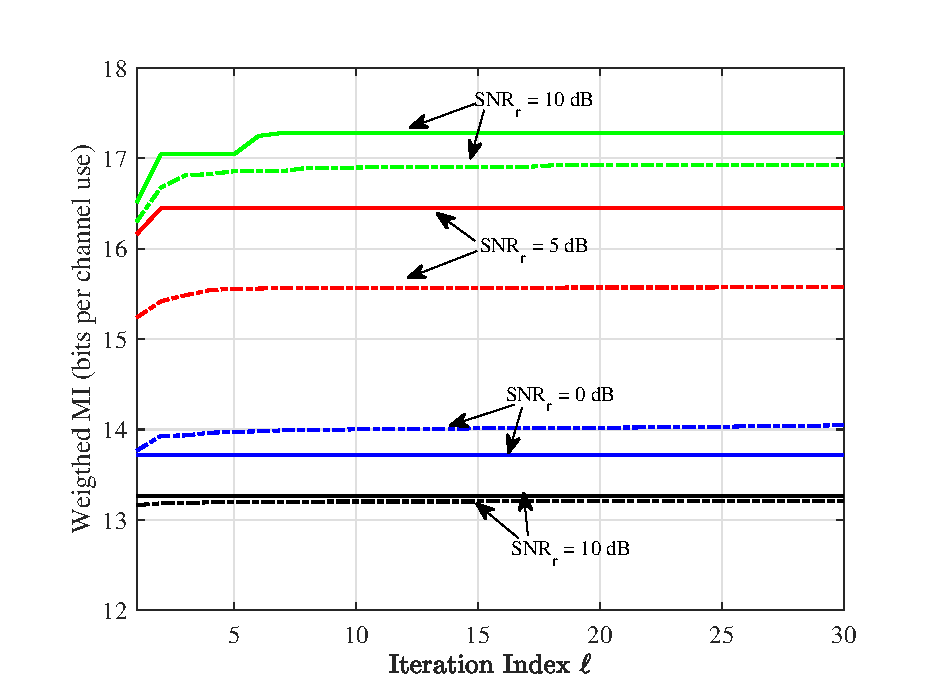
\includegraphics[width=1\columnwidth]{tsp_convergence_snr_nolegend.eps}
	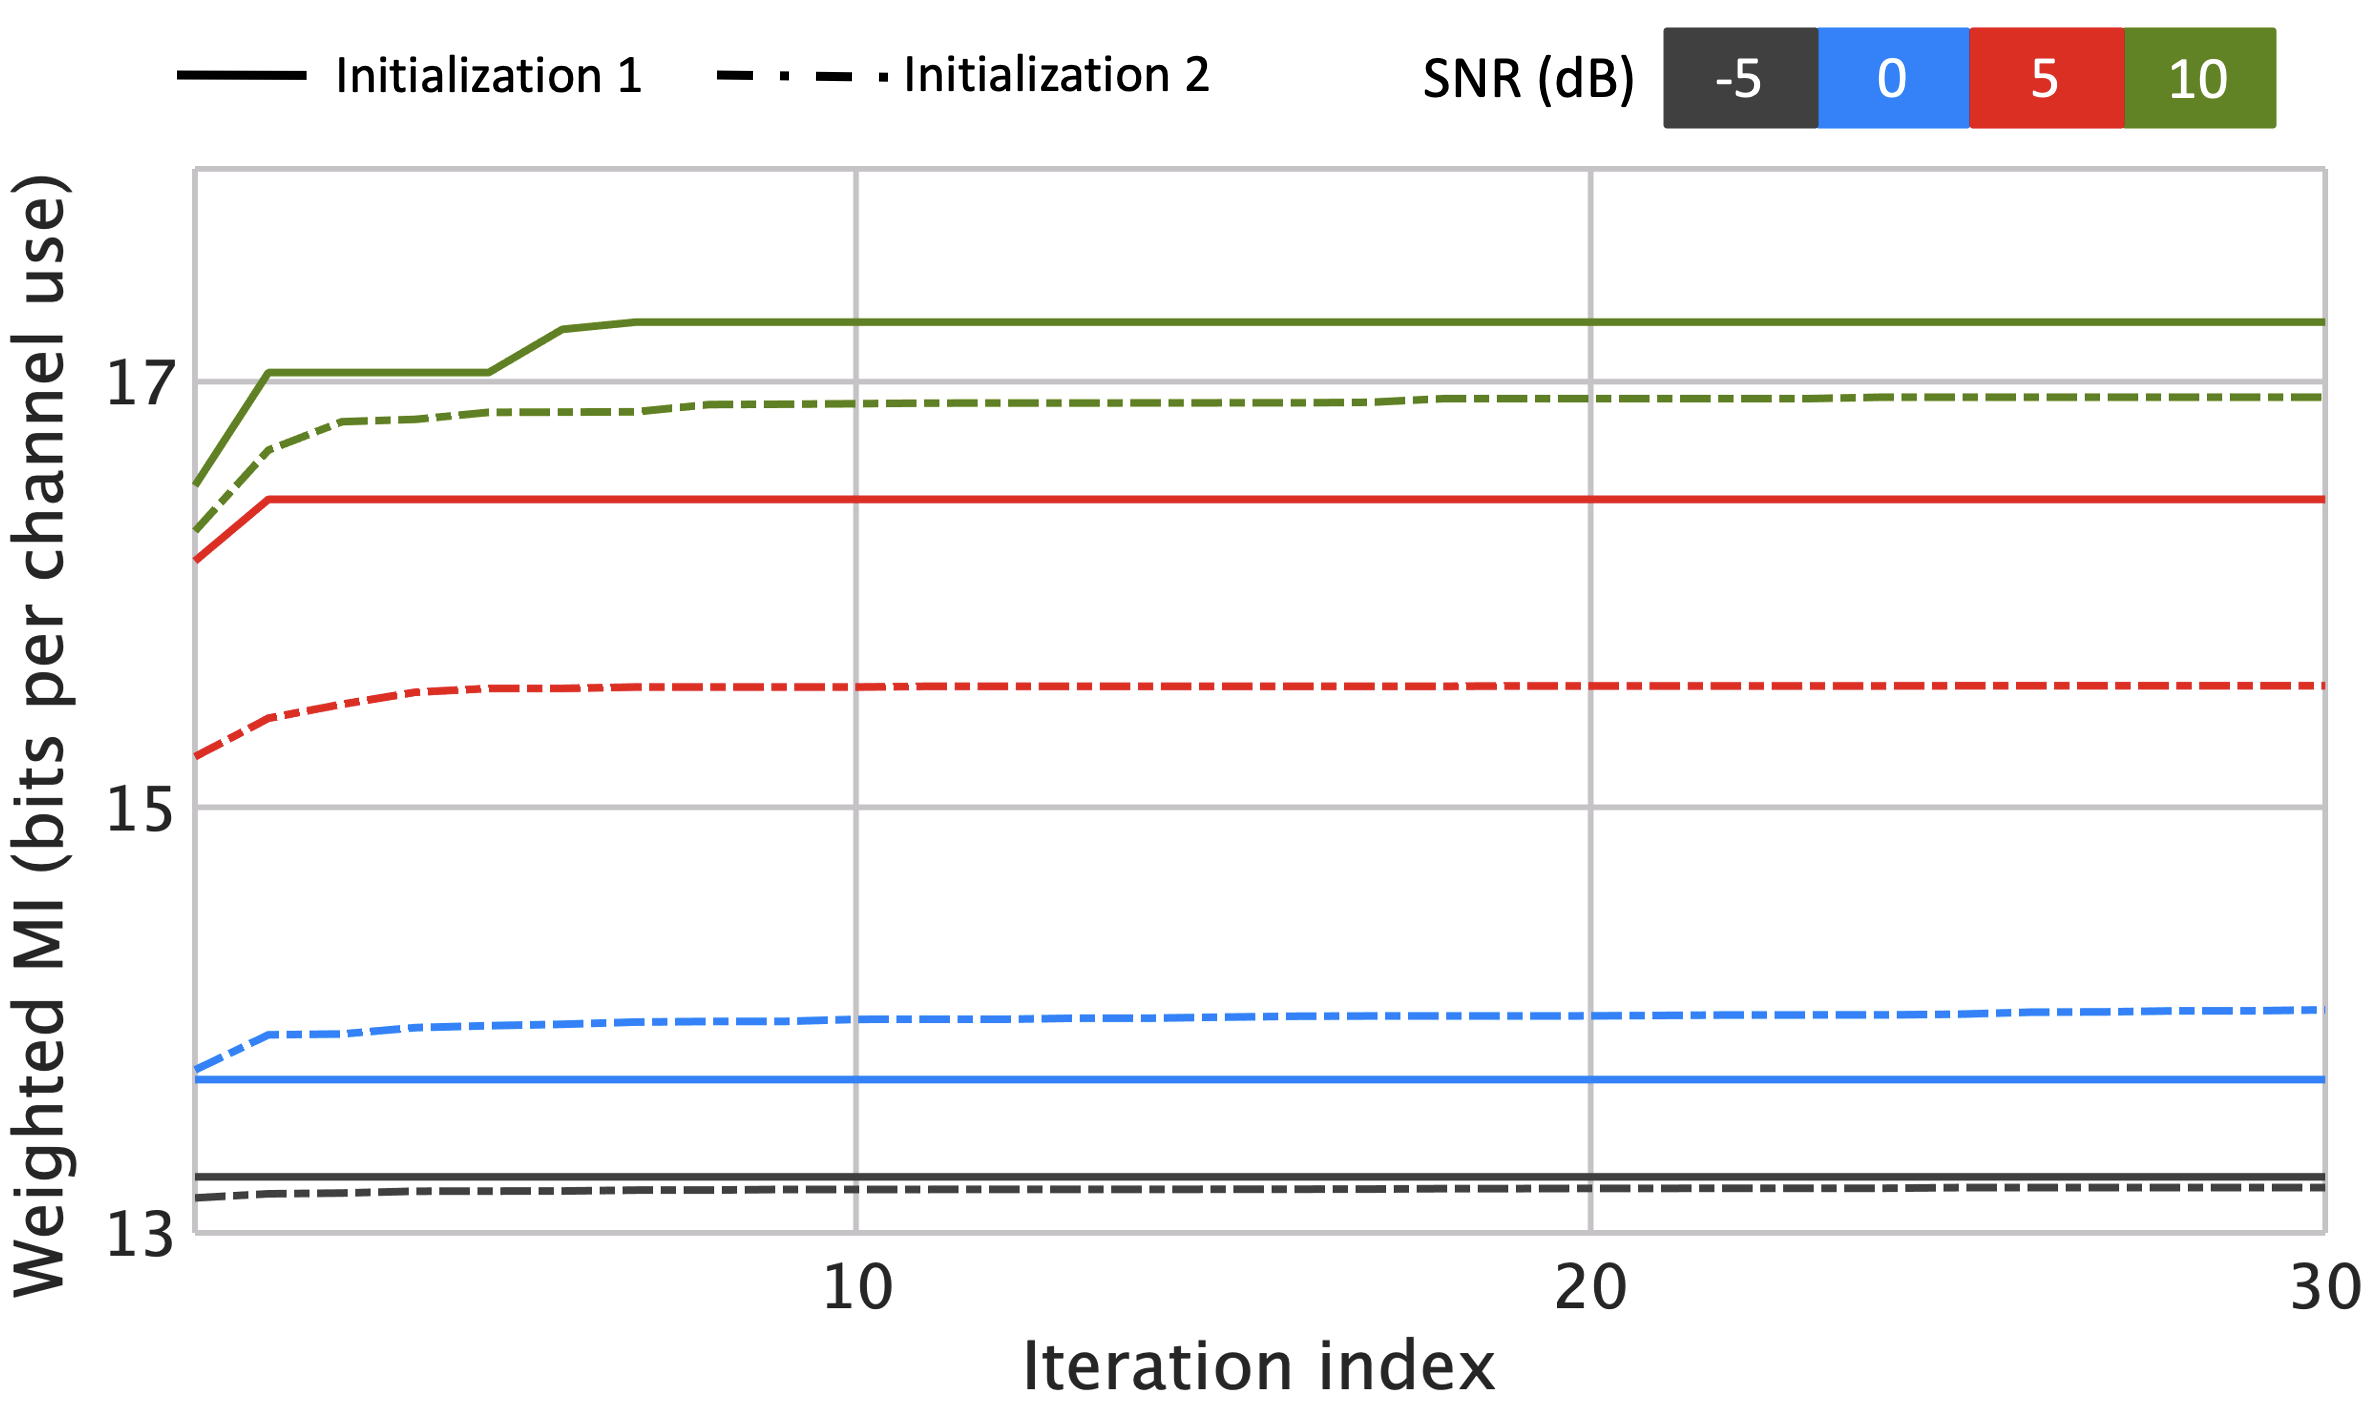
\includegraphics[width=1.0\columnwidth]{tsp_convergence_v03.png}
	%\vspace{-pt}
	\caption{Convergence behaviors of the BCD-AP MRMC algorithm with two initialization methods and multiple $\mathrm{SNR}_\textrm{r}$ values.}
	\label{fig:convergence}
	\vspace{-1em}
\end{figure}
\iffalse
\begin{figure}[!ht]
\centering
\subfloat[$\mathrm{SNR}_\textrm{r}=0\textrm{ dB}$ ]{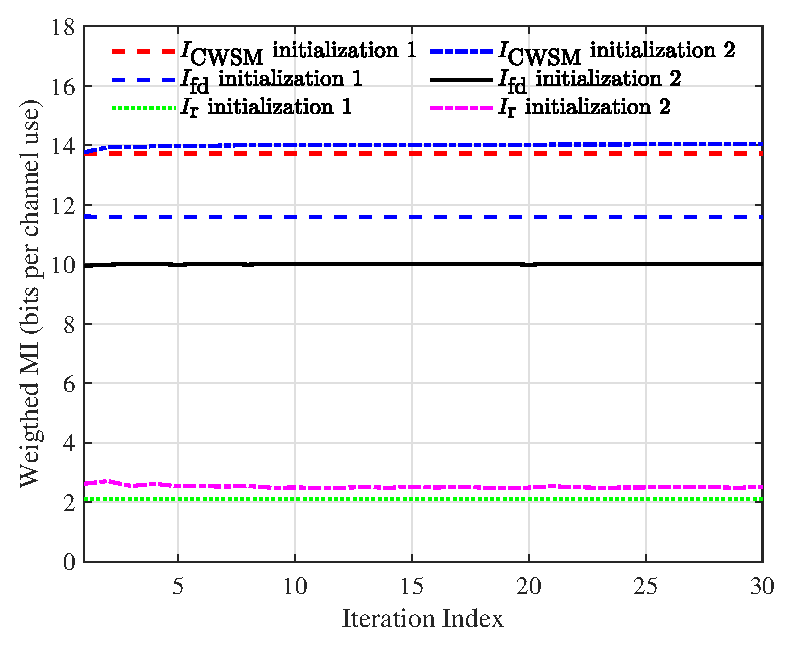
\includegraphics[width=0.45\linewidth]{tsp_convergence_0dB.eps}
\label{fig: con_0dB}}
\hfil
\subfloat[$\mathrm{SNR}_\textrm{r}=10\textrm{ dB}$]{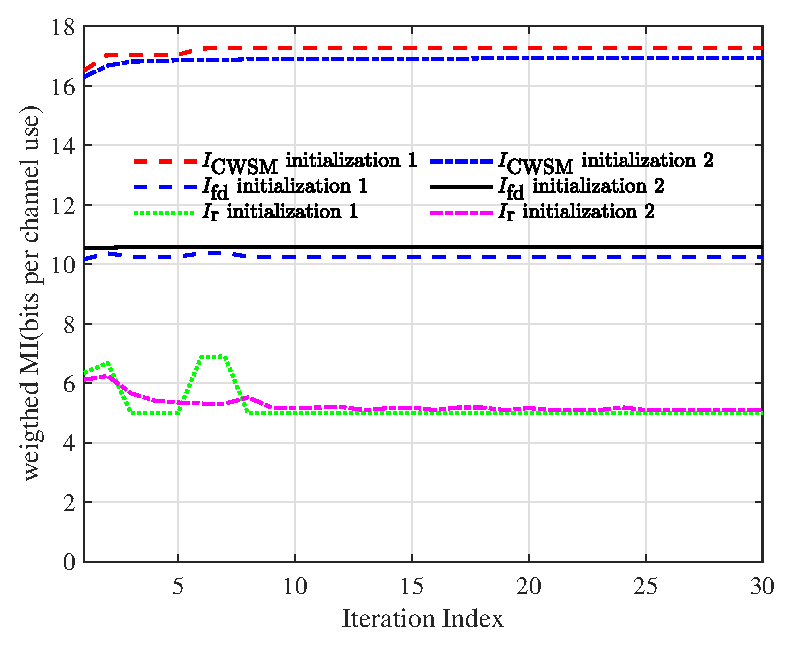
\includegraphics[width=0.45\linewidth]{tsp_convergence_10dB.eps}
\label{fig: con_5dB}}
\caption{Convergence behaviors of Algorithm $\ref{Alternating_sum}$ with two initialization methods}
\label{fig: convergence}
\vspace{-1em}
\end{figure}
\fi
\vspace{-1em}
\subsection{Radar Detection Performance}
%-------------------------------------------------------------
\begin{figure}[t]
%\vspace{-1em}
\centering
%\subfloat[$\mathit{P}_{\textrm{d}}$ versus $\nu$ ]{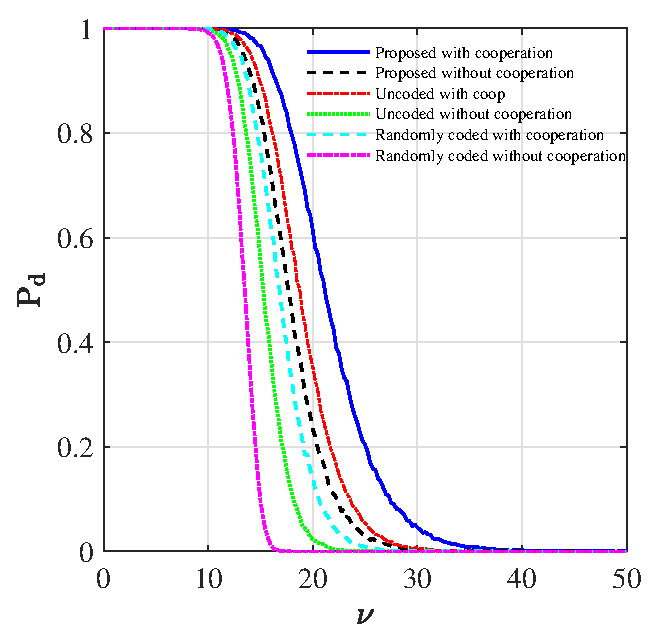
\includegraphics[width=0.48\linewidth]{tsp_pd_vs_vu.eps}
%\label{fig: pd_vs_vu}}
%\hfil
%\subfloat[ROC of the NP detector]{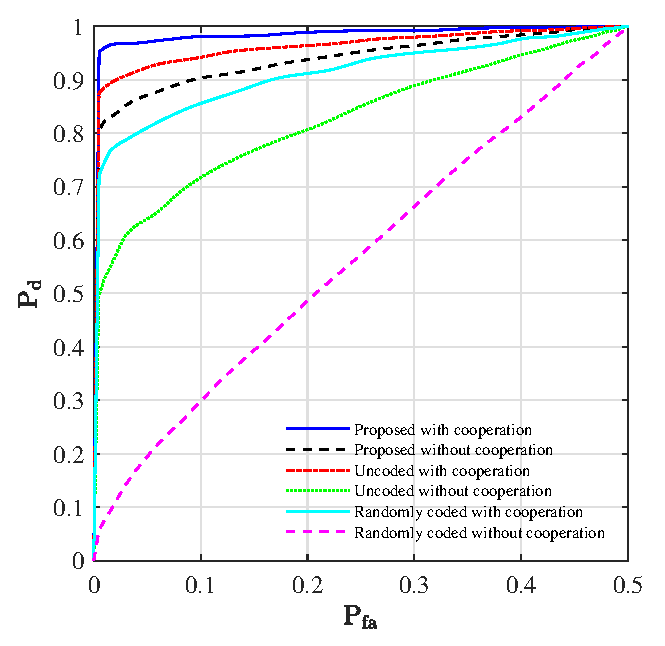
\includegraphics[width=0.48\linewidth]{tsp_ROC.eps}
%\label{fig: roc}}
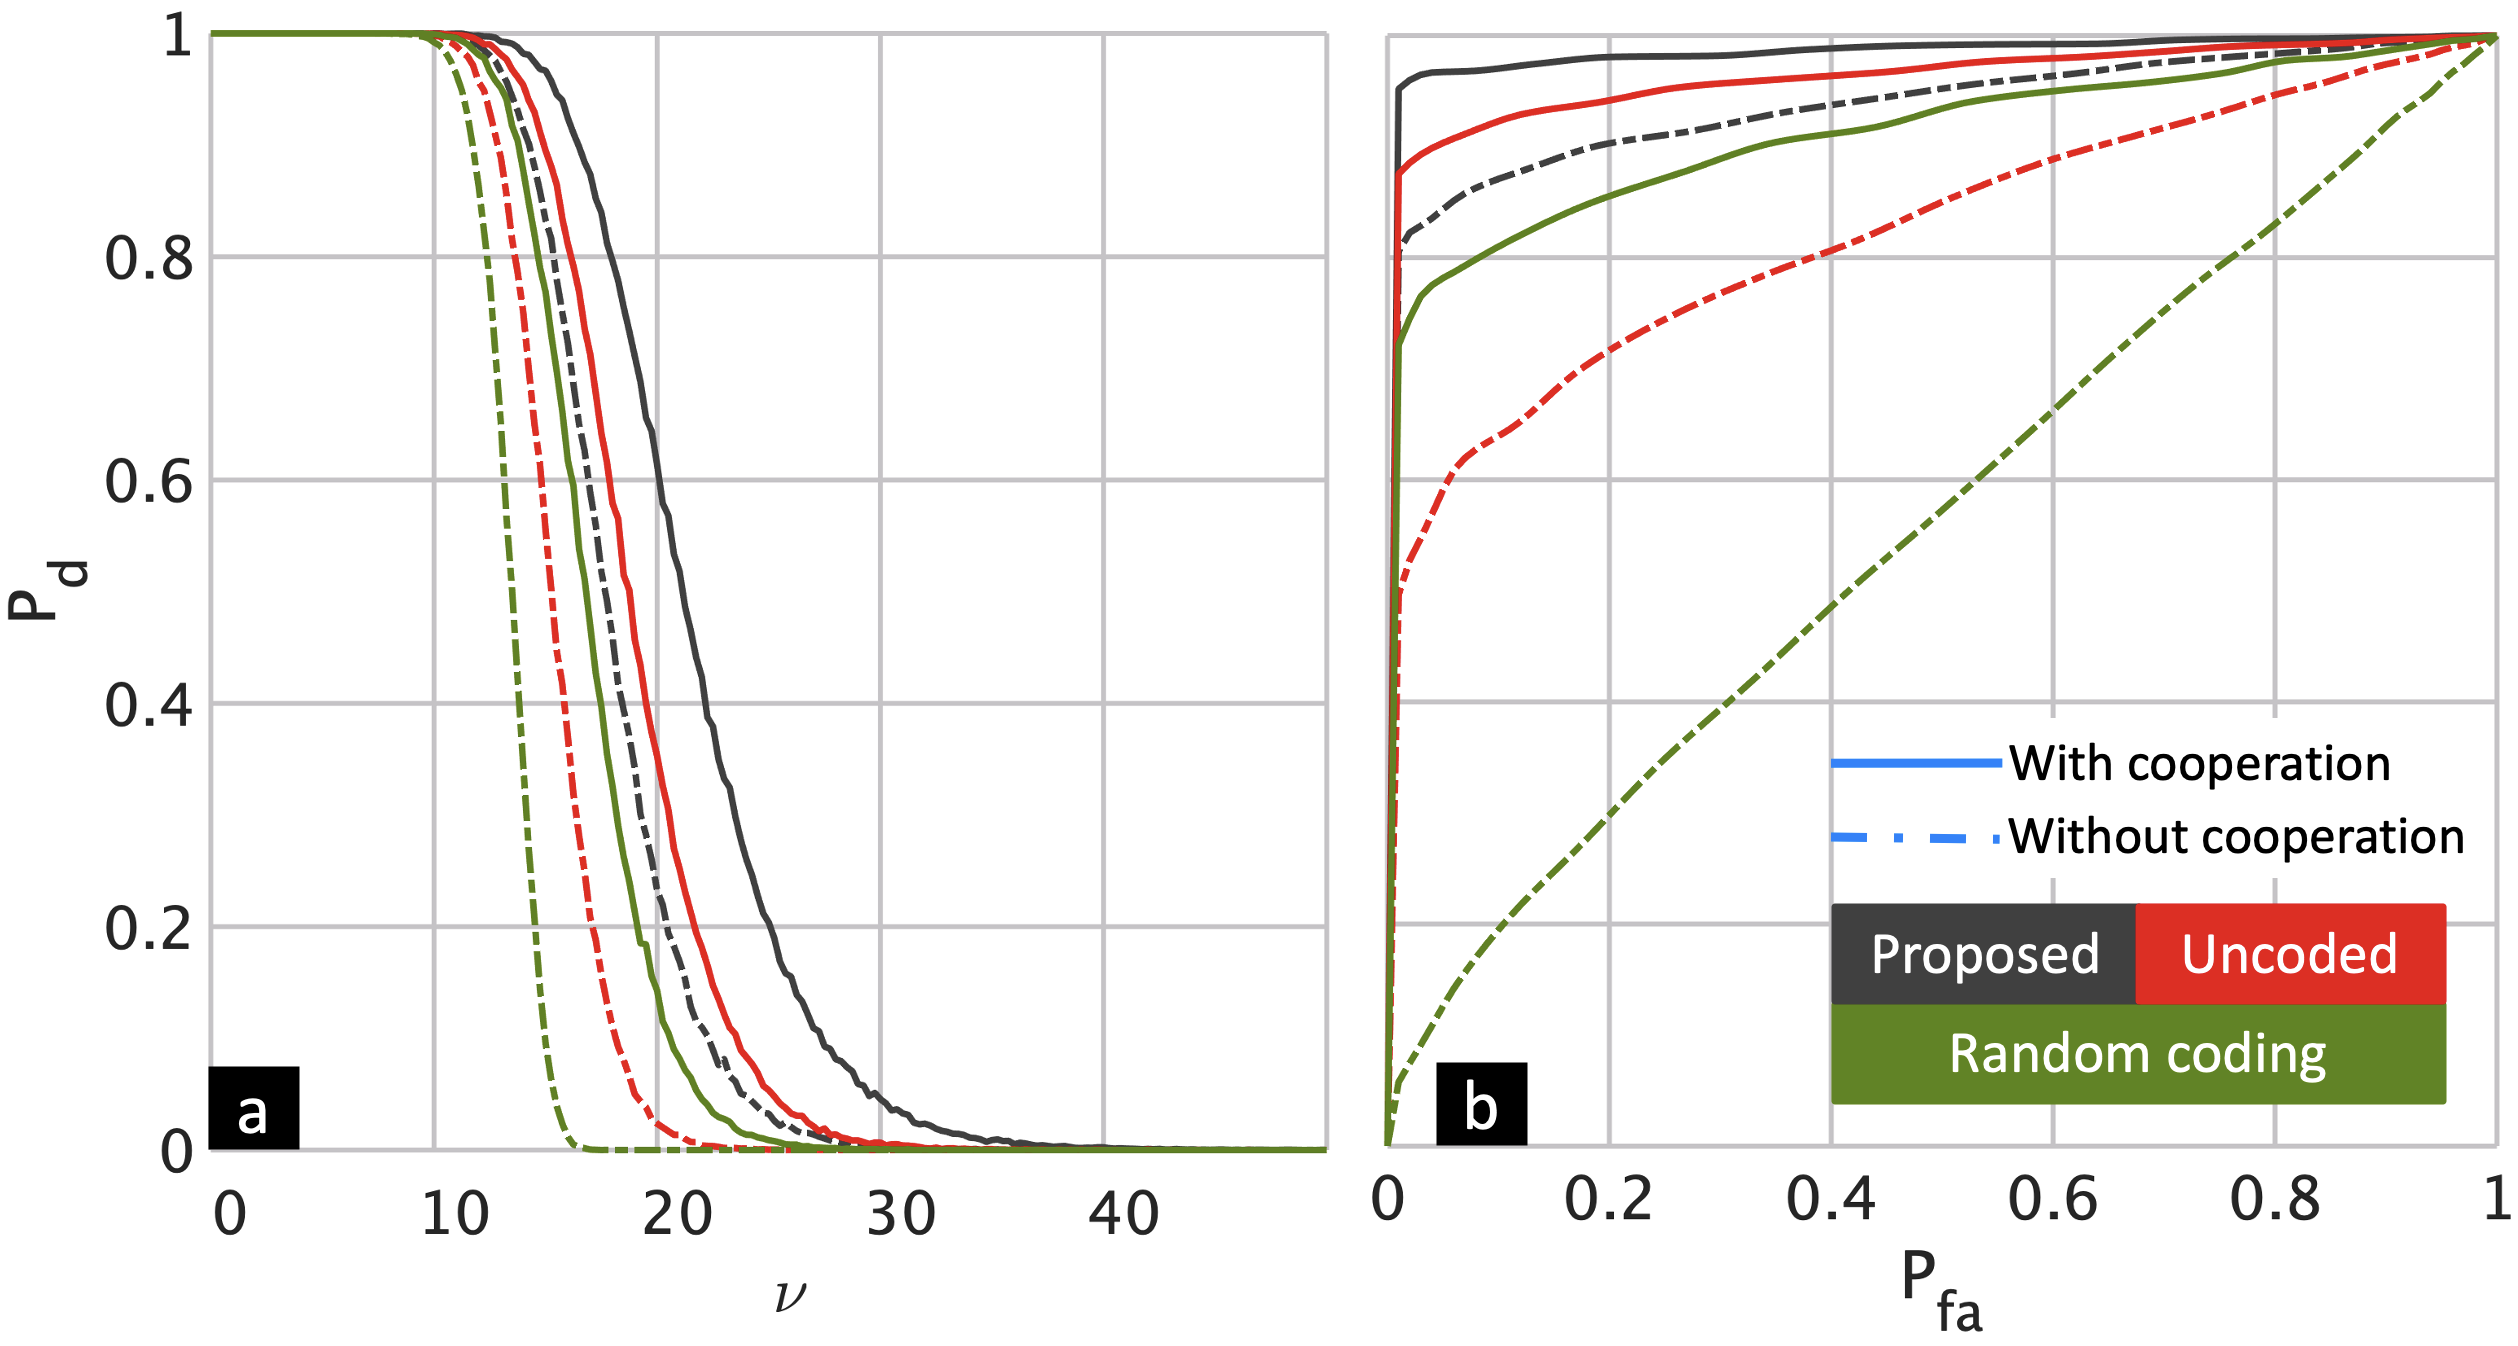
\includegraphics[width=1.0\columnwidth]{NPdetector.png}
\caption{Target detection performance of the coexisting system compared with other radar codes and cooperation schemes using the NP detector. (a) $\mathit{P}_{\textrm{d}}$ versus $\nu$ (b) ROC of the NP detector.}
\label{fig: NPdetector}
\vspace{-1em}
\end{figure}
%-------------------------------------------------------------
We investigated the detection performance of the statistical MIMO radar using the designed code matrix $\mathbf{A}$. % based on a Newman-Pearson (NP) detector. 
Consider the binary hypothesis testing formulation for target detection as
\par\noindent\small
\begin{equation}
\label{eq: hypothesis}
\begin{cases}
\mathcal{H}_{\mathrm{0}}: & \mathbf{y}_{\textrm{r}} = \mathbf{y}_{\textrm{cr}}+\mathbf{y}_{\textrm{Bmr}}+\mathbf{y}_{\textrm{Ur}}+\mathbf{z}_{\textrm{r}}
\\
\mathcal{H}_{\mathrm{1}}: & \mathbf{y}_{\mathrm{r}} = \mathbf{y}_{\textrm{tr}}+ \mathbf{y}_{\textrm{cr}}+\mathbf{y}_{\textrm{Bmr}}+\mathbf{y}_{\textrm{Ur}}+\mathbf{z}_{\textrm{r}},
\end{cases}
\end{equation}
%$\mathbf{y}_{\textrm{cr}}=\bracket{\mathbf{y}^\top_{\textrm{c},1};\cdots;\mathbf{y}^\top_{\textrm{c},\mathit{N}\rr}}^\top$, $\mathbf{y}_{\textrm{Bmr}}=\bracket{\mathbf{y}^\top_{\textrm{Bm},1};\cdots;\mathbf{y}^\top_{\textrm{Bm},\mathit{N}\rr}}^\top$, $\mathbf{y}_{\textrm{Ur}}=\bracket{\mathbf{y}^\top_{\textrm{Ur},1};\cdots;\mathbf{y}^\top_{\textrm{Ur},\mathit{N}\rr}}^\top$, $\mathbf{z}_{\textrm{r}}=\bracket{\mathbf{z}^\top_{\textrm{r},1};\cdots;\mathbf{z}^\top_{\textrm{r},\mathit{N}\rr}}^\to p$, and $\mathbf{y}_{\textrm{tr}}=\bracket{\mathbf{y}^\top_{\textrm{tr},1};\cdots;\mathbf{y}^\top_{\textrm{tr},\mathit{N}\rr}}^\top$.  whose CMs can be written as  $\mathbf{R}_{\mathrm{t}}=\oplus_{n\rr=1}^{\mathit{N}\rr}\mathbf{R}_{\textrm{t},n\rr}$, $\mathbf{R}_{\mathrm{c}}=\oplus_{n\rr}^{\mathit{N}\rr}$
%Notice that the $\mathbf{y}_{\mathrm{c},\textrm{r}}$, $\mathbf{y}_{\mathrm{Bm}}$, $\mathbf{y}_{\mathrm{U}}$, and $\mathbf{z}$ are all zero mean Gaussian random vectors  with CMs being $\mathbf{R}_{\mathrm{t}}=\oplus_{n\rr=1}^{\mathit{N}\rr}\mathbf{R}_{\textrm{t},n\rr}$, $\mathbf{R}_{\mathrm{c}}=\oplus_{n\rr}^{\mathit{N}\rr}$. 
\iffalse
\begin{equation}
\label{eq: hypothesis}
\begin{cases}
\mathrm{H}_{\mathrm{0}}: & \mathbf{y}_{\mathrm{r}} = \mathbf{y}^\textrm{r}_{\textrm{in}}
\\
\mathrm{H}_{\mathrm{1}}: & \mathbf{y}_{\mathrm{r}} = \mathbf{y}_{\mathrm{t}}+ \mathbf{y}^\textrm{r}_{\textrm{in}},
\end{cases}
\end{equation}
where $\mathbf{y}_{\mathrm{r}}=\bracket{\mathbf{y}^\top_{\textrm{r},1};\cdots;\mathbf{y}^\top_{\textrm{r},\mathit{N}\rr}}^\top$ and $\mathbf{y}^\textrm{r}_{\textrm{in}}=\bracket{\paren{\mathbf{y}^{\textrm{r}}_{\textrm{in},n\rr}}^\top;\cdots;\paren{\mathbf{y}^{\textrm{r}}_{\textrm{in},\mathit{N}\rr}}^\top}^\top$,
\fi
where $\mathbf{y}_{\mathrm{r}}=\bracket{\mathbf{y}^\top_{\textrm{r},1};\cdots;\mathbf{y}^\top_{\textrm{r},\mathit{N}\rr}}^\top$ and $\mathbf{y}_{\textrm{tr}}=\bracket{\mathbf{y}^\top_{\textrm{tr},1};\cdots;\mathbf{y}^\top_{\textrm{tr},\mathit{N}\rr}}^\top$. Denote $\mathbf{y}^\textrm{r}_{\textrm{in}}\triangleq\mathbf{y}_{\textrm{cr}}+\mathbf{y}_{\textrm{Bmr}}+\mathbf{y}_{\textrm{Ur}}+\mathbf{z}_{\textrm{r}}=\bracket{\paren{\mathbf{y}^{\textrm{r}}_{\textrm{in},n\rr}}^\top;\cdots;\paren{\mathbf{y}^{\textrm{r}}_{\textrm{in},\mathit{N}\rr}}^\top}^\top$ and its CM $\mathbf{R}_{\textrm{in}}=\oplus_{n\rr=1}^{N\rr}\mathbf{R}_{\textrm{in},n\rr}$. Similarly, define $\overline{\mathbf{y}}_{\textrm{r},n\rr} = \mathbf{R}^{-\sfrac{1}{2}}_{\textrm{in},n\rr}\mathbf{y}_{\textrm{r},n\rr}$ and its CM $\mathbf{G}_{n\rr}=\mathbf{R}^{-\sfrac{1}{2}}_{\textrm{in},n\rr}\mathbf{R}_{\textrm{t},n\rr}\mathbf{R}^{-\sfrac{1}{2}}_{\textrm{in},n\rr}$. Rewrite hypothesis testing problem as  \par\noindent\small
%If $\mathbf{M}_{n\rr}\triangleq\mathbf{R}_{\textrm{in},n\rr }$ and  , the test problem can be rewritten as 
\begin{equation}
\begin{cases}
\mathcal{H}_{\mathrm{0}}: & \overline{\mathbf{y}}_{\mathrm{r}}\sim\mathcal{CN}\paren{\mathbf{0},\mathbf{I}}
\\
\mathcal{H}_{\mathrm{1}}: & \overline{\mathbf{y}}_{\mathrm{r}}\sim\mathcal{CN}\paren{\mathbf{0},\mathbf{I}+\mathbf{G}},
\end{cases}
\end{equation}\normalsize
where the block diagonal matrix $\mathbf{G}=\oplus_{n\rr=1}^{\mathit{N}\rr}\mathbf{G}_{n\rr}$. The eigendecomposition of $\mathbf{G}_{n\rr}$ is $\mathbf{G}_{n\rr}=\mathbf{V}_{n\rr}\mathbf{\Lambda}_{n\rr}\mathbf{V}^\dagger_{n\rr}$, where the columns of $\mathbf{V}_{n\rr}$ and the diagonal entries of $\mathbf{\Lambda}_{n\rr}\triangleq\diag\bracket{\delta_{1,n\rr},\cdots,\delta_{\mathit{K},n\rr}}$ are, respectively, the eigenvectors and eigenvalues of $\mathbf{G}_{n\rr}$, the $\ith{k}$ eigenvalue being $\delta_{k,n\rr}$. Using the Woodbury matrix identity and the eigendecomposition of $\mathbf{G}_{n\rr}$, the test statistic is\par\noindent\small
\begin{flalign}
T\paren{\overline{\mathbf{y}}}&=\sum_{n\rr=1}^{\mathit{N}\rr}T\paren{\overline{\mathbf{y}}_{\textrm{r},n\rr}}=\sum_{n\rr=1}^{\mathit{N}\rr}\overline{\mathbf{y}}^\dagger_{\textrm{r},n\rr}\paren{\mathbf{I}-\paren{\mathbf{G}_{n\rr}+\mathbf{I}}^{-1}}\overline{\mathbf{y}}_{\textrm{r},n\rr}\nonumber\\
&=\sum_{n\rr=1}^{\mathit{N}\rr}\overline{\mathbf{y}}^\dagger_{\textrm{r},n\rr}\mathbf{V}_{n\rr}\paren{\mathbf{\Lambda}^{-1}+\mathbf{I}}^{-1}\mathbf{V}^\dagger_{n\rr}\overline{\mathbf{y}}_{\textrm{r},n\rr}
\end{flalign}\normalsize
Denote $\widehat{\mathbf{y}}_{\textrm{r},n\rr}=\mathbf{V}^\dagger_{n\rr}\overline{\mathbf{y}}_{\textrm{r},n\rr}=\bracket{\widehat{y}_{n\rr}\bracket{1},\cdots,\widehat{y}_{n\rr}\bracket{\mathit{K}}}$. Then, the Neyman-Pearson (NP) detector is\cite{Kay1993detection}
\begin{equation}
\label{eq: NPdetector}
%\sum_{n\rr}^{\mathit{N}\rr}T\paren{\overline{\mathbf{y}}_{\textrm{r},n\rr}}
T\paren{\overline{\mathbf{y}}}=\sum_{n\rr=1}^{\mathit{N}\rr}\sum_{k=1}^{\mathit{K}}\frac{\delta_{k,n\rr}\lvert\widehat{y}_{n\rr}\bracket{k}\rvert^2}{1+\delta_{k,n\rr}}\underset{\mathrm{H}_2}{\overset{\mathrm{H}_1}{\gtrless}}\nu,
\end{equation}
where $\nu$ is the threshold selected to guarantee a certain detection performance. We performed Monte Carlo (MC) simulations to evaluate the probability of detection $\mathit{P}_{\textrm{d}}$ and the Rx operating characteristic (ROC) (curve of $\mathit{P}_{\textrm{d}}$ versus probability of false alarm $\mathit{P}_{\textrm{fa}}$) of the NP detector. Figures~\ref{fig: NPdetector}a and \ref{fig: NPdetector}b show $\mathit{P}_{\textrm{d}}$ with respect to $\nu$ and ROC, %, namely the curve of $\mathit{P}_{\textrm{d}}$ versus the probability of false alarm $\mathit{P}_{\textrm{fa}}$, 
respectively, for various waveforms and cooperation modes. Here, presence or absence of cooperation indicates whether or not the DL signals $\mathbf{y}_{\textrm{Bt},n\rr}$ are incorporated in $\mathbf{y}_{\textrm{t,}n\rr}$ for all $n\rr$. For the $\ith{m\rr}$ radar Tx, the uncoded waveform is $\mathbf{a}_{m\rr}=\sqrt{\frac{\mathit{P}_{\textrm{r},m\rr}}{\mathit{K}}}\mathbf{1}_{\mathit{K}}$ and randomly coded waveform is  $\mathbf{a}_{m\rr}=\sqrt{\frac{\mathit{P}_{\textrm{r},m\rr}}{\mathit{K}}}\mathbf{u}_{m\rr}$, where $\braces{\mathbf{u}_{m\rr}}$ is a unitary basis. We generated $5000$ realizations of $\overline{\mathbf{y}}_{\textrm{r}}$ under hypothesis $\mathcal{H}_1$ to estimate $\mathit{P}_{\textrm{d}}$ and $\mathcal{H}_0$ to estimate $\mathit{P}_{\textrm{fa}}$ based on $\nu$ for each mode. Figures~\ref{fig: NPdetector}a and \ref{fig: NPdetector}b illustrate that our optimized radar waveform outperforms the all-ones (uncoded) and random coding schemes, and that the cooperation between the radar and BS boosts the radar detection performance. For example, in \figurename{\;\ref{fig: NPdetector}b, with $P_{\textrm{fa}}=0.1$, when radar codes and UL/DL precoders obtained via Algorithm \ref{Alternating_sum} are used along with radar-DL cooperation, this yields approximately $8\%$ improvement in $P_{\textrm{d}}$ over the non-cooperation mode, $6\%$ over the all-ones waveform with cooperation, and $13\%$ over randome code with cooperation. We observe that even without the cooperation, our algorithm enables the MIMO radar to provide a competitive detection performance.

\iffalse
\begin{figure}[t]
\centering
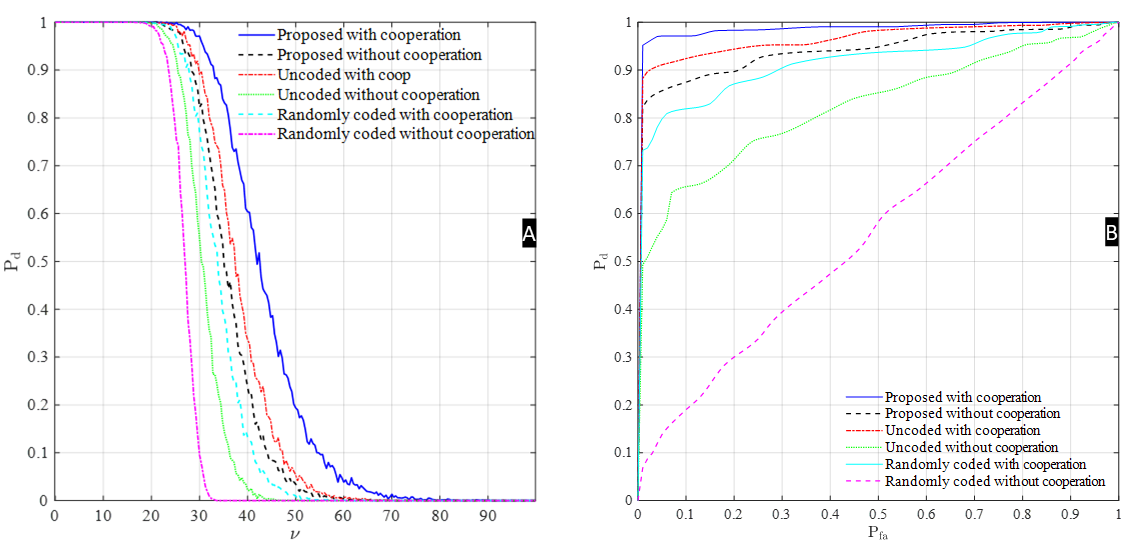
\includegraphics[width=0.45\linewidth]{radar_figures_roc.png}
%\vspace{-14pt}
\caption{$\paren{\textrm{a}}$ $\mathit{P}_{\textrm{d}}$ versus $\nu$ with different combinations of waveform and cooperation schemes $\paren{\textrm{b}}$ the corresponding ROC of the NP detector}
\label{fig: NPdetector}
\end{figure}
\fi
\vspace{-1em}
\subsection{FD Communications Performance}
\label{subsec: fd_comm_eva}
\begin{figure}[t]
\vspace{-1em}
\centering
%\subfloat[Weighted MI versus various number of UL UEs]{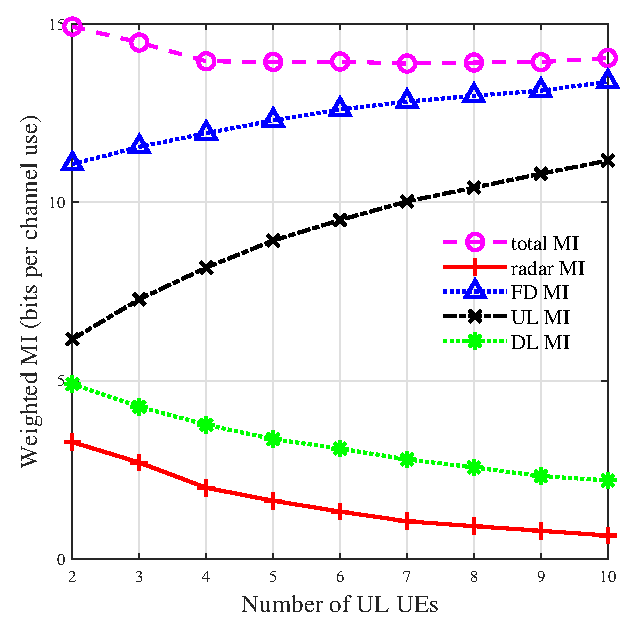
\includegraphics[width=0.48\linewidth]{II.eps}
%\label{fig: UL_UE}}
%\hfil
%\subfloat[Weighted MI versus various number of DL UEs]{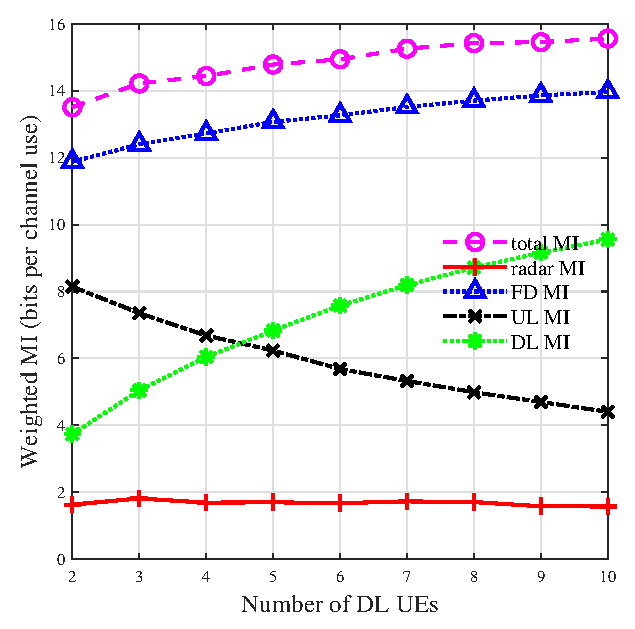
\includegraphics[width=0.48\linewidth]{tsp_DL_UE.eps}
%\label{fig: DL_UE}}
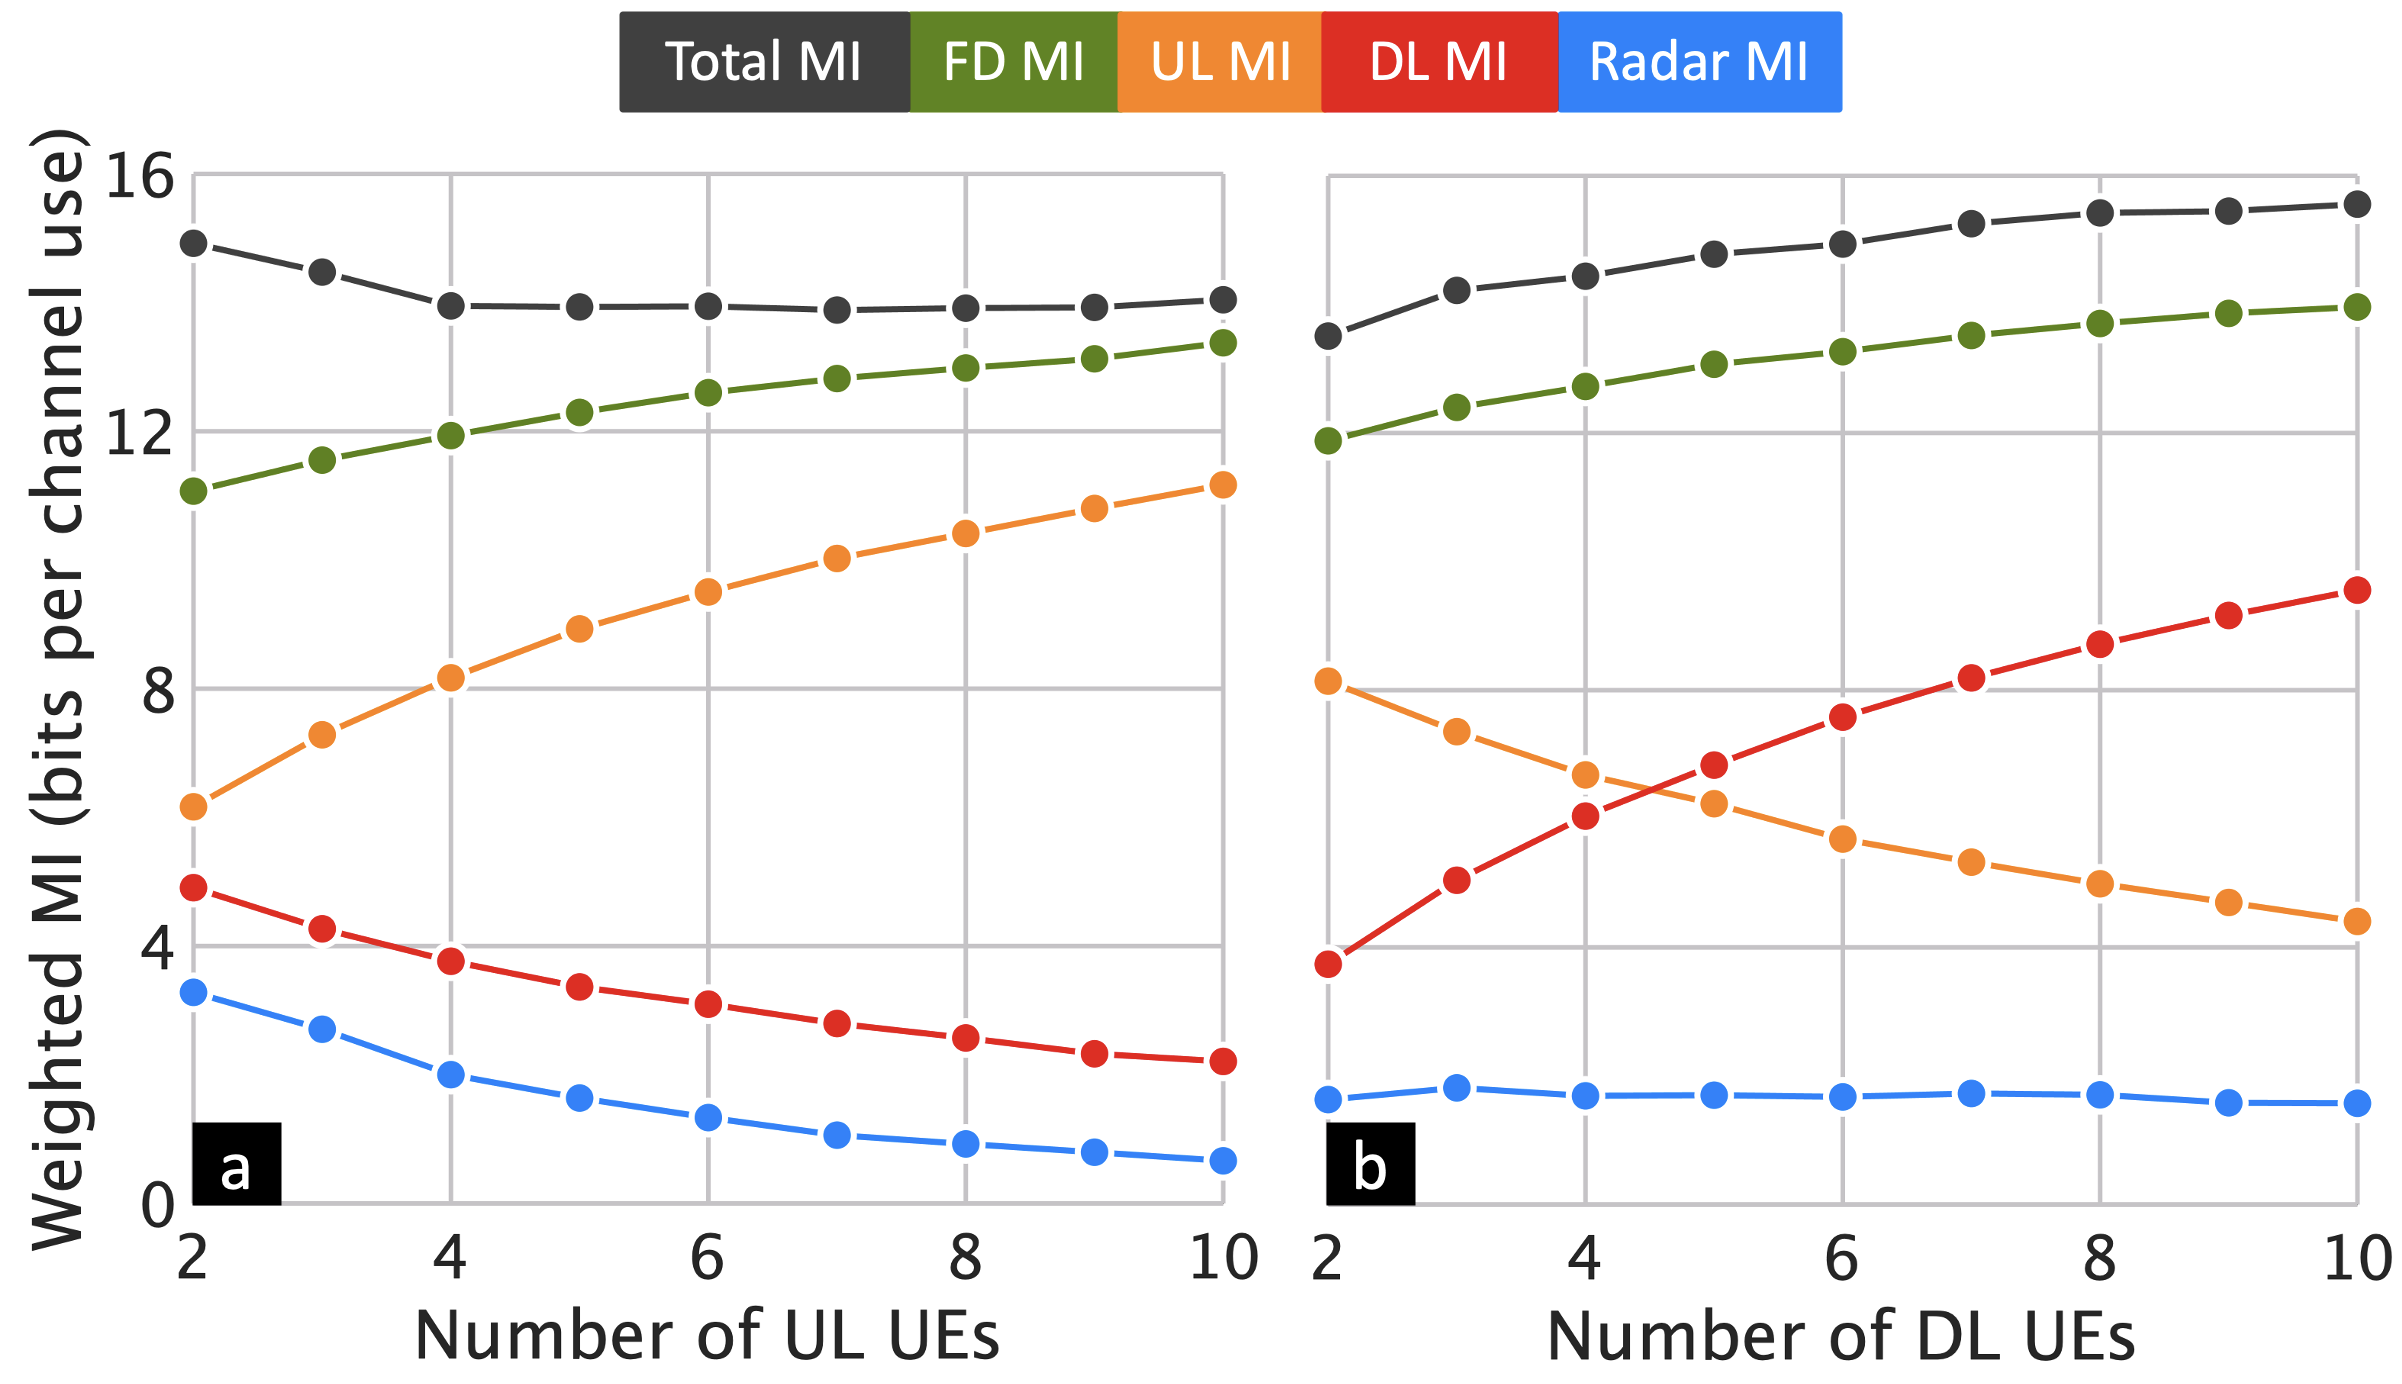
\includegraphics[width=0.9\columnwidth]{fd_UE.png}
\caption{Performance of the coexisting system evaluation compared with increasing numbers of (a) UL and (b) DL UEs.}
\label{fig:fd_UE}
\vspace{-1em}
\end{figure}
%-------------------------------------------------------------
We explored the effect on the system performance with increasing UEs. Figures~\ref{fig:fd_UE}a and \ref{fig:fd_UE}b depict weighted UL MI $\mathit{I}_{\textrm{U}}\triangleq\sum_{k}\sum_{i}\alpha^\textrm{u}_i\mathit{I}_{\textrm{u},i}\bracket{k}$, weighted DL MI $\mathit{I}_{\textrm{D}}\triangleq\sum_{k}\sum_{j}\alpha^\textrm{d}_j\mathit{I}_{\textrm{d},j}\bracket{k}$, radar MI $\mathit{I}_{\textrm{R}}\triangleq\alpha^\textrm{r}_{n\rr}\sum_{n\rr}\mathit{I}_{\textrm{r},n\rr}\bracket{k}$, total weighted FD MI and $\mathit{I}_{\textrm{CWSM}}$ as the number of UL UEs and DL UEs are varied, respectively. The power levels are set at $\mathit{P}_{\textrm{u}}=I$ and $\mathit{P}_{\textrm{d}}=J$. As the number of UL UEs 
increases from $\mathit{I}=2$ to $\mathit{I}=10$ with the number of DL UEs fixed at $\mathit{J}=2$, the performances of DL UEs and radar Rxs deteriorate owing to the increasing UL interference. On the other hand, the performance of the UL drops while that of the MIMO radar remains relatively stable as the number of DL UEs rises from $\mathit{J}=2$ to $\mathit{J}=10$ with $\mathit{I}=2$. We observe that the total system performance measure  $\mathbf{I}_{\textrm{CWSM}}$ is enhanced with a higher DL power because of the radar-DL cooperation whereas $\mathbf{I}_{\textrm{CWSM}}$ declines with a rising UL power. 

\vspace{-1em}
\subsection{Joint Radar-Communications Performance}
%-------------------------------------------------------------
\begin{figure}[t]
	\centering
	%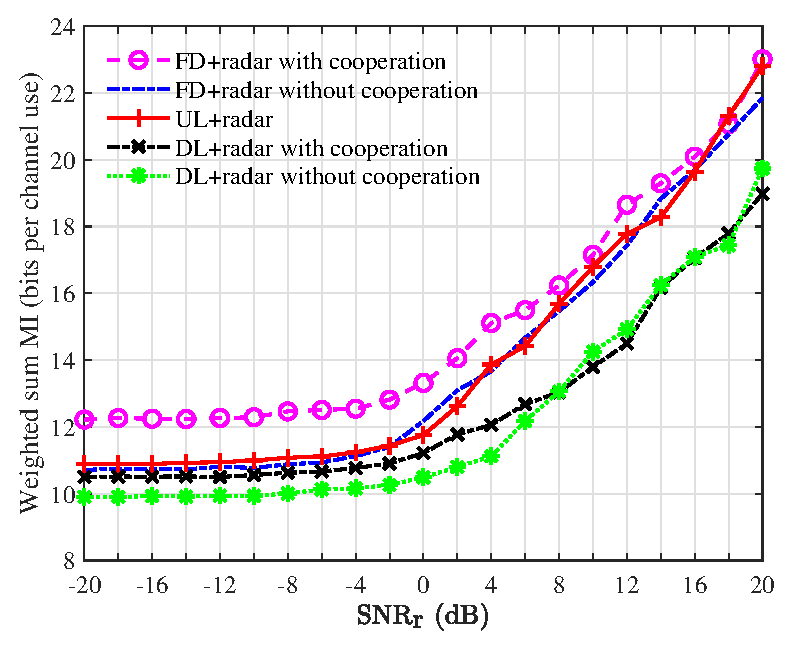
\includegraphics[width=1\columnwidth]{fd_vs_hd.eps}
	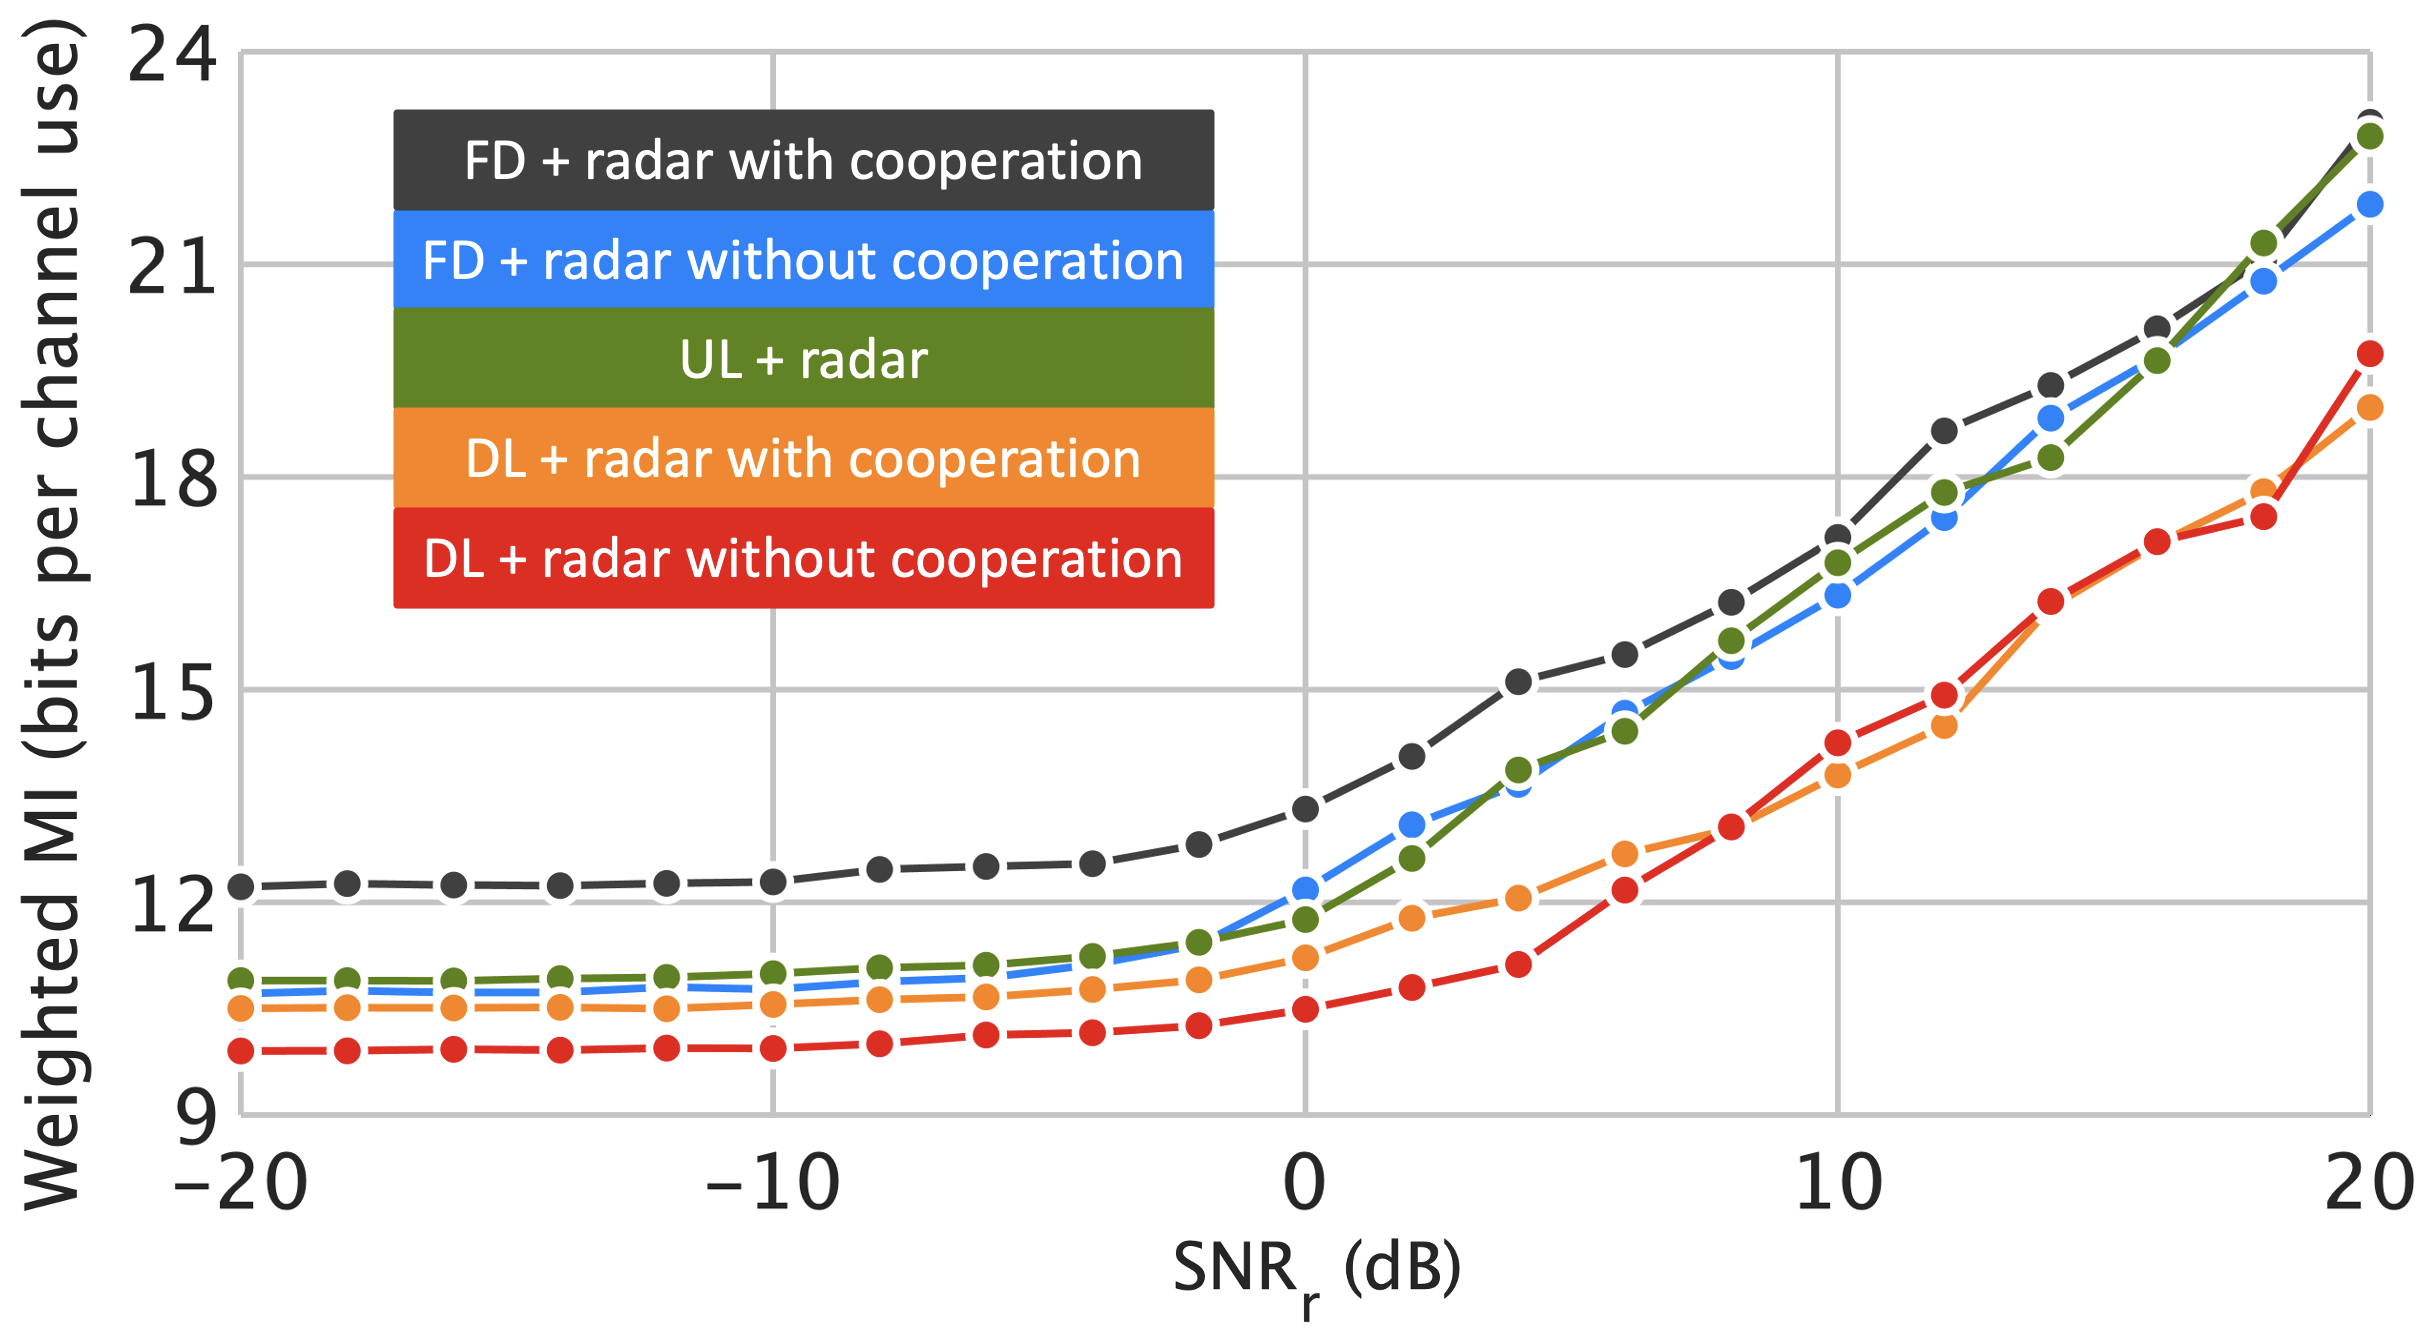
\includegraphics[width=1.0\columnwidth]{fd_vs_hd_v03.png}
	%\vspace{-pt}
	\caption{Evaluation of the MU-MIMO communications with different transmission schemes under various radar SNRs}
	\label{fig:fd_vs_hd}
	\vspace{-1em}
\end{figure}
%-------------------------------------------------------------
\begin{figure}[t]
\centering
%\subfloat[System performance vs UL SNRs]{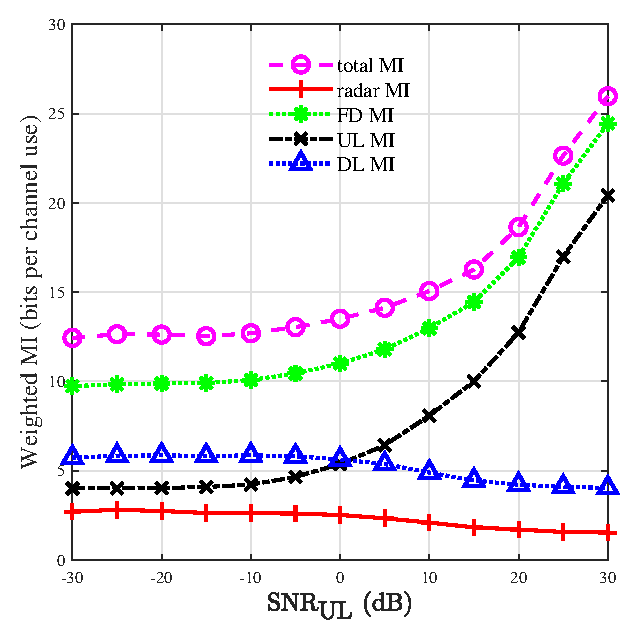
\includegraphics[width=0.48\columnwidth]{UL_SNR_sweep.eps}
%\label{fig: UL_SNR}}
%\hfil
%\subfloat[System performance vs CNR]{\includegraphics[width=0.48\columnwidth]{CNR_sweep.eps}
%\label{fig: CNR}}
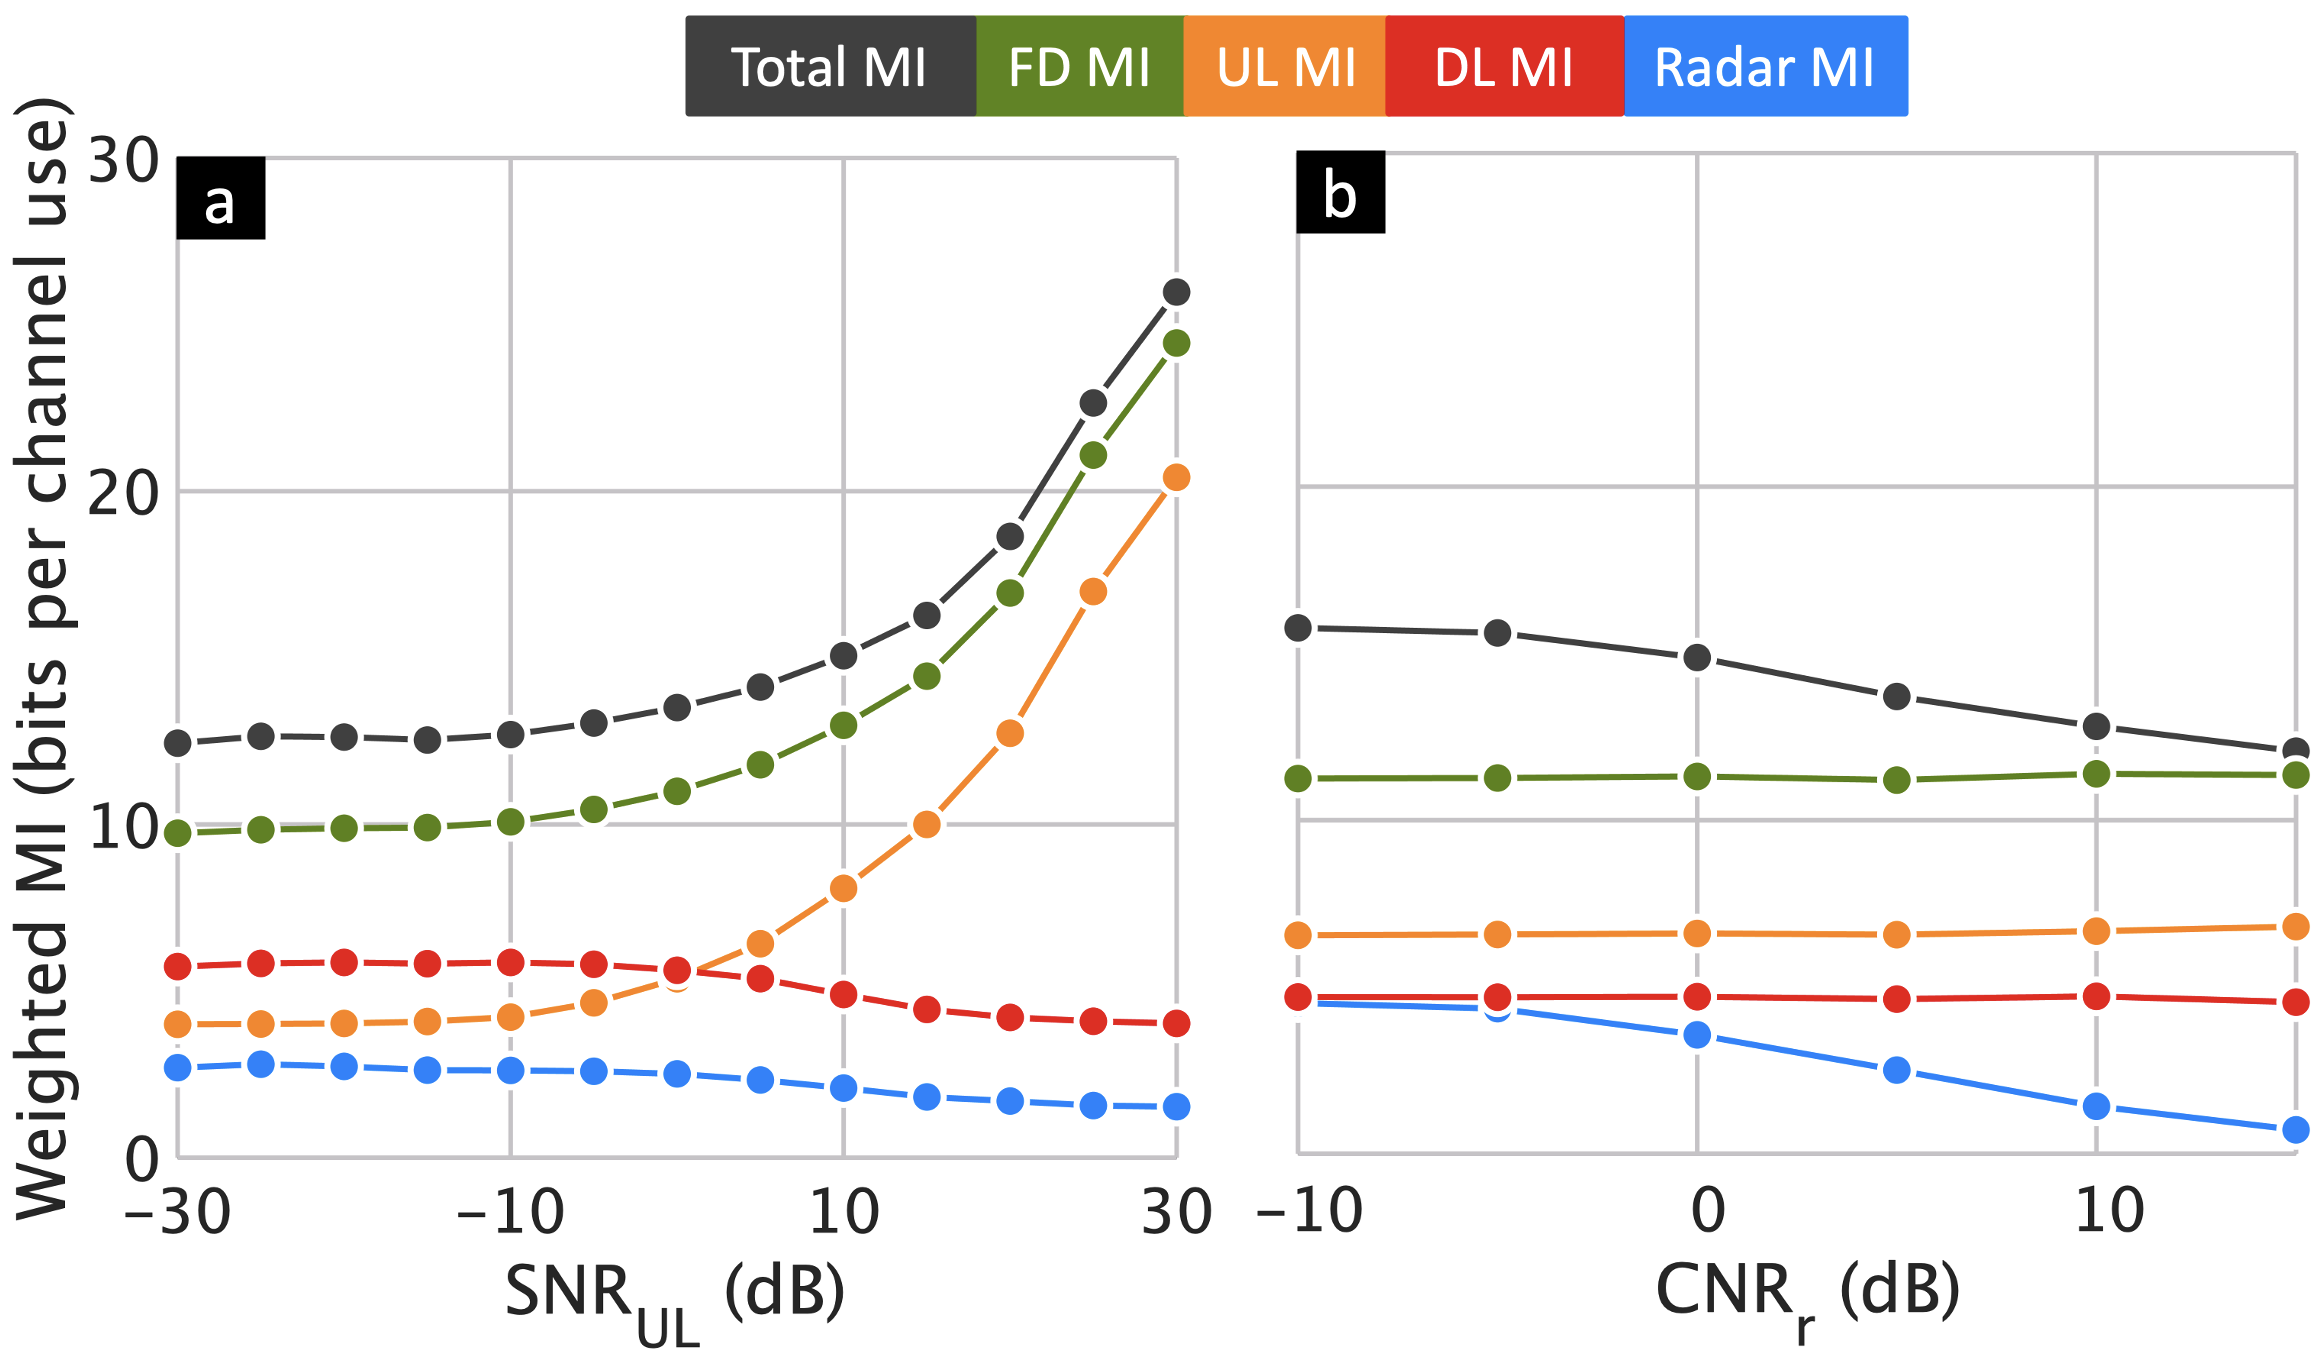
\includegraphics[width=0.9\columnwidth]{joint.png}
\caption{Joint radar and communications interference analysis. (a) System performance vs UL SNRs (b) System performance vs CNR.}
\label{fig:joint}
\vspace{-1em}
\end{figure}
\iffalse
%-------------------------------------------------------------
\begin{figure}[t]
\centering
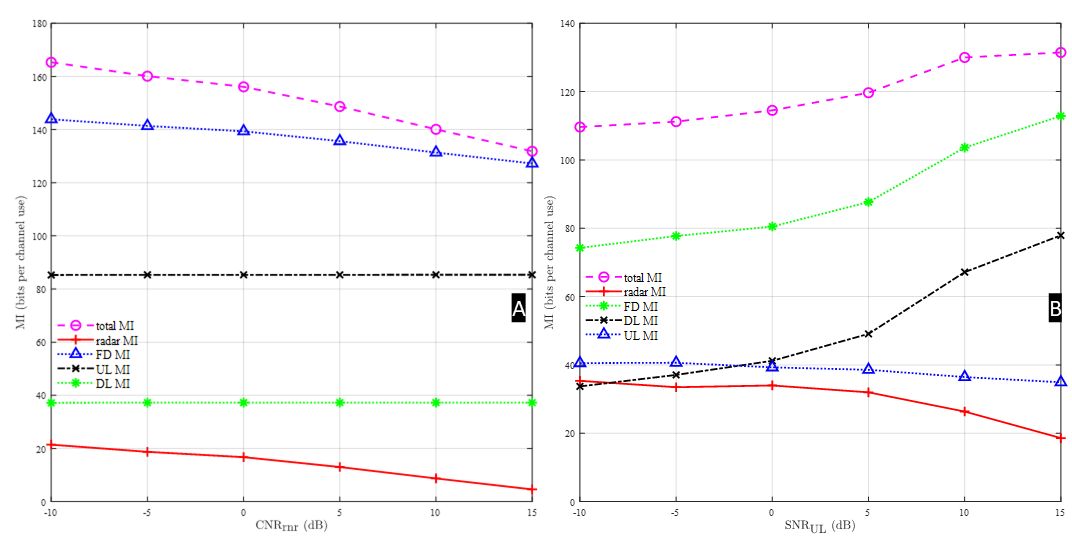
\includegraphics[width=1\columnwidth]{radar_figures_cnr.png}
%\vspace{-14pt}
\caption{$\paren{\textrm{a}}$ MI achieved by Algorithm $\ref{Alternating_sum}$ versus different $\mathrm{CNRs}$   $\paren{\textrm{b}}$ MI achieved by Algorithm $\ref{Alternating_sum}$ versus various UL $\mathrm{SNR}$ }
\label{fig:cnr}
\vspace{-1em}
\end{figure}
%-------------------------------------------------------------
\fi
Finally, we evaluated the co-design performance by observing the mutual impact of the statistical MIMO radar and IBFD MU-MIMO communications on each other. Figure~\ref{fig:fd_vs_hd} compares the CWSMs achieved by the IBFD MU-MIMO as well as the HD MU-MIMO communications jointly operating with a statistical MIMO radar. We also included the cooperation and non-cooperation modes for IBFD MU-MIMO and DL MU-MIMO communications. In practice, the radar-enabled interference channel gains, namely $\eta^2_{\mathrm{r},j}$ and $\eta^2_{\mathrm{rB}}$ are fractions of the radar-target channel gains $\eta^2_{m\rr,n\rr}$. As a result, the severity of the radar-enabled interference with the communications systems are also related to the radar-target channel gains. Specifically, we set $\mathrm{SNR}_{\textrm{r}}=0.8\mathrm{SNR}_{\textrm{rB}}$ and $\mathrm{SNR}_{\textrm{r}}=0.6\mathrm{SNR}_{\textrm{rd}}$. We observed that when the radar power dominates the co-designed system, the impact of radar-DL cooperation is less apparent. In \figurename{\;\ref{fig:joint}}, the performance of co-designed system is shown to vary with different UL SNR and CNR values.  %Like the assumption we made with \figurename{\;\ref{fig:fd_vs_hd}}, 
Here, $\mathrm{SNR}_{\textrm{ur}}=0.7\mathrm{SNR}_{\textrm{u}}$ and  $\mathrm{SNR}_{\textrm{ud}}=0.8\mathrm{SNR}_{\textrm{u}}$ for Fig.~\ref{fig:joint}a  and $\mathrm{SNR}_{\textrm{rB}}=0.5\mathrm{CNR}_{\textrm{r}}$ and $\mathrm{SNR}_{\textrm{rd}}=0.5\mathrm{CNR}_{\textrm{r}}$ for Fig.~\ref{fig:joint}b.  Note that the DL and radar weighted MIs decline by approximately $30\%$ and $45\%$, respectively, when the UL-DL and UL-radar interfering signal powers are $10^6$ times higher. This demonstrates that the designed precoders and radar codes sustain the DL and radar performances despite a high UL Tx power. Meanwhile, from Fig.~\ref{fig:joint}b, the clutter affects the MIMO radar more than the FD communications UEs because the proposed method mitigates the power projected to the interfering channels $\mathbf{H}_{\textrm{rB}}$ and $\mathbf{H}_{\textrm{r,}j}$ from $\braces{\mathbf{a}\bracket{k}}$.
% $\eta_{\mathrm{u},i}$ and $\eta_{\mathrm{d},i}$ are fractions of $\eta^2_{i,n\rr}$ and $\eta_{m\rr,\B}$ and $\eta_{m\rr,j}$ are fractions of $\sigma^2_{\textrm{c},n\rr}$. 
\vspace{-1em}
%\section{Conclusion}
\section{Summary}
\label{sec:conclusion}
%\textcolor{red}{Need to make this shorter}
In this work, we proposed a spectral co-design for a statistical MIMO radar and an IBFD MU-MIMO communications system. Prior works either largely consider co-located MIMO radars, focus on coexistence solutions, or partially analyze MIMO communications. We take a wholesome view of the problem by jointly designing several essential aspects of such a co-design:  UL/DL precoders, MIMO radar code matrix, and LRFs for both systems. Our proposed BCD-AP MRMC algorithm not only guarantees convergence but also provides performance benefits for both systems. %First, we demonstrate the rapid convergence of the BCD-AP MRMC algorithm with two different initializations. Second, 
The radar codes generated by BCD-AP MRMC significantly increase the probability of detection over conventional waveforms. We also showed that the cooperation between radar and DL signals is beneficial for target detection. The co-designed DL and radar are resilient to considerable UL interference. Similarly, using our optimized precoders and radar codes, the DL and UL rates remain stable as the CNR is increased. %Based on our theoretical and numerical results, we conclude that our algorithm is a superior approach to achieve the spectral co-design for the co-existence of a statistical MIMO radar and an IBFD MU-MIMO communications system. 
%For the future work, we would address the impact of the CSI errors on both the MIMO radar and IBFD MU-MIMO communications and develop a robust version of the proposed framework.
%such that the MIMO radar and the FD MU-MIMO communications system can operate simultaneously on the same spectrum while maintaining their respective performances.
	%  if have a single appendix:
	%\appendix[Proof of the Zonklar Equations]
	% or
	%\appendix  % for no appendix heading
	% do not use \section anymore after \appendix, only \section*
	% is possibly needed
	% use appendices with more than one appendix
	% then use \section to start each appendix
	% you must declare a \section before using any
	% \subsection or using \label (\appendices by itself
	% starts a section numbered zero.)
	%
	
%\vspace{-1em}	
\appendices
\section{Proof of Theorem \ref{theorem: dual}}
\label{appendix:theorem2}
Solving $\paren{\ref{dualproblem}}$ yields the lower bounds of $\paren{\ref{WMMSE2}}$. The difference between the lower bound and the actual optimal value is the optimal duality gap. To equivalently obtain $\braces{\mathbf{P}^\star}$ and $\mathbf{A}^\prime$ with $\paren{\ref{dualproblem}}$, strong duality ought to hold for the primal problem $\paren{\ref{WMMSE1}}$, i.e., the optimal duality gap needs to be zero. However, the QoS constraints $\paren{\mathrm{\ref{UL_rate}}}-\paren{\mathrm{\ref{DL_rate}}}$ are non-concave leading to a non-zero duality gap. To bypass this problem, we apply the Taylor series to obtain linear approximations of $\mathit{R}_{\textrm{u},i}\bracket{k}$ and $\mathit{R}_{\textrm{d},j}\bracket{k}$. The first-order Taylor series expansion of a real-valued function with complex-valued matrix arguments $f\paren{\mathbf{X},\mathbf{X}^\ast}: \mathbb{C}^{\mathit{N}\times \mathrm{Q}}\times\mathbb{C}^{\mathit{N}\times \mathrm{Q}}\rightarrow\mathbb{R}$ around $\mathbf{X}_{\mathrm{0}}$ produces \cite{hjorungnes2011complex} \par\noindent\small
\begin{flalign}
\label{eq: Taylor}
f\paren{\mathbf{X},\mathbf{X}^\ast} &= f\paren{\mathbf{X}_{\mathrm{0}},\mathbf{X}^\ast_{\mathrm{0}}}+\vect^\top\paren{\frac{\partial }{\partial \mathbf{X}_{\mathrm{0}}}f\paren{\mathbf{X}_{\mathrm{0}},\mathbf{X}^\ast_{\mathrm{0}}}}\vect\paren{\mathbf{X}-\mathbf{X}_{\mathrm{0}}}\nonumber\\
&+\vect^\top\paren{\frac{\partial }{\partial \mathbf{X}^\ast_{\mathrm{0}}}f\paren{\mathbf{X}_{\mathrm{0}},\mathbf{X}^\ast_{\mathrm{0}}}}\vect\paren{\mathbf{X}^\ast-\mathbf{X}^\ast_{\mathrm{0}}}.
\end{flalign}\normalsize
Assume $\widetilde{\mathbf{P}}_{\textrm{u},i}\bracket{k}$ is the estimate of $\PiB$ from the previous iteration. A similar Taylor series expansion of $\mathit{R}_{\textrm{u},i}\bracket{k}$ at $\widetilde{\mathbf{P}}_{\textrm{u},i}\bracket{k}$ gives \par\noindent\small
\begin{IEEEeqnarray}{rCl}
&&\mathit{R}_{\textrm{u},q}\bracket{k}\paren{\PiB}\approx \mathit{R}_{\textrm{u},q}\bracket{k}\paren{\widetilde{\mathbf{P}}_{\textrm{u},i}\bracket{k}}+\nonumber\\
&&\vect\braces{\frac{\partial \paren{\mathit{R}_{\textrm{u},q}\bracket{k}\paren{\widetilde{\mathbf{P}}^\ast_{\textrm{u},i}\bracket{k}}}}{\partial \widetilde{\mathbf{P}}_{\textrm{u},i}\bracket{k}}}^\top\vect\braces{\PiB-\widetilde{\mathbf{P}}_{\textrm{u},i}\bracket{k}}+\nonumber\\
&&\vect\braces{\frac{\partial \paren{\mathit{R}_{\textrm{u},q}\bracket{k}\paren{\widetilde{\mathbf{P}}_{\textrm{u},i}\bracket{k}}}}{\partial \widetilde{\mathbf{P}}^\ast_{\textrm{u},i}\bracket{k}}}^\top \vect\braces{\mathbf{P}^\ast_{\textrm{u},i}\bracket{k}-\widetilde{\mathbf{P}}^\ast_{\textrm{u},i}\bracket{k}}.
\end{IEEEeqnarray}\normalsize

Likewise, we find the linear approximations of $\mathit{R}_{\textrm{u},q}\bracket{k}\paren{\PBj}$, $\mathit{R}_{\textrm{u},q}\bracket{k}\paren{\mathbf{a}\bracket{k}}$, $\mathit{R}_{\textrm{d},j}\bracket{k}\paren{\PiB}$, $\mathit{R}_{\textrm{d},j}\bracket{k}\paren{\PBj}$, and $\mathit{R}_{\textrm{d},j}\bracket{k}\paren{\mathbf{a}\bracket{k}}$.  
Note that $\Xi_{\text{wmmse}}$ is multi-convex, namely $\Xi_{\text{wmmse}}$ is not jointly convex in $\PiB$, $\PBj$, and $\mathbf{a}\bracket{k}$ but convex in each individual variable provided the rest of the variables are fixed \cite{FD_WMMSE,BCDconvergence}. As a result, we have a fully convex version of $\paren{\ref{WMMSE2}}$ and thus the optimal duality gap between $\paren{\ref{WMMSE2}}$ and $\paren{\ref{dualproblem}}$ is reduced to zero \cite{Lui2006subg}. 
Hence, $\braces{\mathbf{P}^\star}$ and $\mathbf{A}^\prime=\bracket{\paren{\mathbf{a}^\prime\bracket{1}}^\top,\cdots,\paren{\mathbf{a}^\prime\bracket{\mathit{K}}}^\top}$ in $\paren{\ref{WMMSE2}}$ are obtained by solving $\paren{\ref{dualproblem}}$. This concludes the proof.
%\vspace{-1em}
\section{Derivation of Gradients}
\label{app:grad}
Adopting the notations from \cite{hjorungnes2011complex} and \cite{IMM2012-03274}, we denote the complex gradient operator for a scalar real-valued function with a complex-valued matrix argument $f\paren{\mathbf{Z},\mathbf{Z^\star}}$ as $\nabla_\mathbf{Z}f=\frac{\partial f}{\partial\mathbf{Z}^\ast}$. From the derivative formula $\frac{\partial}{\partial \mathbf{X}^\ast}\trace\paren{\mathbf{B}^\top\mathbf{X}^\dagger\mathbf{CXB}}=\mathbf{C}^\top\mathbf{XBB}^\top+\mathbf{CXBB}^\top $ \cite{IMM2012-03274}, the gradients of $\Xi_{\text{UL}}$ and $\Xi_{\text{DL}}$ with respect to $\PiB$, $\PBj$ and $\mathbf{a}\bracket{k}$, respectively, are \par\noindent\small
%\begin{flalign}
\begin{IEEEeqnarray}{rCl}\label{GD_constraint}
	\IEEEyesnumber\IEEEyessubnumber*
	\nabla_{\PiB}\Xi_{\textrm{UL}}&=&\HiBH\boldsymbol{\xi}_{\textrm{UL}}\mathbf{H}_{i,\B}\PiB, \\
	\nabla_{\PBj}\Xi_{\text{UL}}&=&\HBBH\boldsymbol{\xi}_{\textrm{UL}}\HBB\PBj,\\
	\nabla_{\mathbf{a}\bracket{k}}\Xi_{\text{UL}}&=&\HrBH\boldsymbol{\xi}_{\textrm{UL}}\HrB\mathbf{a}\bracket{k},\\
	\nabla_{\PiB}\Xi_{\text{DL}}&=&\sum_{g=1}^\mathit{J}\mathbf{H}^\dagger_{i,g}\boldsymbol{\xi}_{\textrm{d},g}\mathbf{H}_{i,g}\PiB,\\
	\nabla_{\PBj}\Xi_{\text{DL}}&=&\sum_{g=1}^{\mathit{J}}\mathbf{H}^\dagger_{\B,g}\boldsymbol{\xi}_{\textrm{d},g}\mathbf{H}_{\B,g}\PBj\\
	%&&+\mathbf{H}^\dagger_{\B,j}\UBjH\mathbf{W}^\dagger_{\B,j}\bracket{k}\UBj\mathbf{H}_{\B,j}\PBj\nonumber\\
	%&-2\mathbf{H}^\dagger_{\B,j}\UBjH\mathbf{W}^\dagger_{\B,j}\bracket{k}&
	\textrm{and }\nabla_{\mathbf{a}\bracket{k}}\Xi_{\text{DL}}&=&\sum_{g=1}^{\mathit{J}}\HrgH\boldsymbol{\xi}_{\textrm{d},g}\Hrg\mathbf{a}\bracket{k},
	%\end{flalign}
\end{IEEEeqnarray}\normalsize
where $\boldsymbol{\xi}_{\textrm{UL}}\bracket{k}=\sum_{q=1}^{\mathit{I}}\alpha^\textrm{u}_q\UqBnH\WqB\UqB$ and  $\boldsymbol{\xi}_{\textrm{d},g}\bracket{k}=\alpha^\textrm{d}_g\mathbf{U}^\dagger_{\textrm{d},g}\bracket{k}\mathbf{W}_{\textrm{d},g}\bracket{k}\mathbf{U}_{\textrm{d},g}\bracket{k}$.
The gradients of $\Xi_{\text{r}}$ with respect to $\PiB$, $\PBj$, and $\mathbf{a}\bracket{k}$, respectively, are \par\noindent\small
\begin{align}
\nabla_{\PiB}\Xi_{\text{r}}=&\sum_{n\rr=1}^{\mathit{N}\rr}\eta^2_{i,n\rr}\sum_{m=1}^{\mathrm{\mathit{K}}}\mathbf{P}_{\textrm{u},i}\bracket{m}\mathbf{d}_{\textrm{u},i}\bracket{m}\mathrm{\xi}_{n\rr}\paren{m,k}\mathbf{d}^\dagger_{\textrm{u},i}\bracket{k},\nonumber\\
=&\sum_{n\rr=1}^{\mathit{N}\rr}\eta^2_{i,n\rr}\sum_{m\neq k}^{\mathrm{\mathit{K}}}\mathbf{P}_{\textrm{u},i}\bracket{m}\mathbf{d}_{\textrm{u},i}\bracket{m}\mathrm{\xi}_{n\rr}\paren{m,k}\mathbf{d}^\dagger_{\textrm{u},i}\bracket{k}\nonumber\\
&+\sum_{n\rr=1}^{\mathit{N}\rr}\eta^2_{i,n\rr}\mathbf{P}_{\textrm{u},i}\bracket{k}\mathbf{d}_{\textrm{u},i}\bracket{k}\mathrm{\xi}_{n\rr}\paren{k,k}\mathbf{d}^\dagger_{\textrm{u},i}\bracket{k}\nonumber
\end{align}
\begin{align}
\nabla_{\PBj}\Xi_{\text{r}}
=&\sum_{n\rr=1}^{\mathit{N}\rr}\mathbf{J}^\top_{\textrm{B}}\sigmanr\sum_{m=1}^{\mathrm{\mathit{K}}}\mathbf{s}_{\target,n\rr}\bracket{m}\mathrm{\xi}_{n\rr}\paren{m,k}\mathbf{d}^\dagger_{\textrm{d},j}\bracket{k}+\nonumber\\
&\sum_{n\rr=1}^{\mathit{N}\rr}\eta^2_{\textrm{Bm},n\rr}\sum_{m=1}^{\mathrm{\mathit{K}}}\sum_{g=1}^{\mathit{J}}\mathbf{P}_{\textrm{d},g}\bracket{m}\mathbf{d}_{\textrm{d},g}\bracket{m}\mathrm{\xi}_{n\rr}\paren{m,k}\mathbf{d}^\dagger_{\textrm{d},j}\bracket{k},\nonumber\\
\nabla_{\mathbf{a}\bracket{k}}\Xi_{\text{r}}=& \sum_{n\rr=1}^{\mathit{N}\rr}\mathbf{Q}^\dagger\rnr\mathbf{J}^\top_{\textrm{r}}\sigmanr\sum_{m=1}^{\mathrm{\mathit{K}}}\mathbf{s}_{\target,n\rr}\bracket{m}\mathrm{\xi}_{n\rr}\paren{m,k}\nonumber\\
%\mathbf{u}^\top\rnr\bracket{m}\mathbf{W}^\top\rnr\mathbf{u}^\ast\rnr\bracket{k}\nonumber\\
=&\sum_{n\rr=1}^{\mathit{N}\rr}\mathbf{Q}^\dagger\rnr\mathbf{J}^\top_{\textrm{r}}\sigmanr\sum_{m\neq k}^{\mathrm{\mathit{K}}}\mathbf{s}_{\target,n\rr}\bracket{m}\mathrm{\xi}_{n\rr}\paren{m,k}\nonumber\\
&+\sum_{n\rr=1}^{\mathit{N}\rr}\mathbf{a}\bracket{k}\eta^2_{\textrm{rt},n\rr}\mathrm{\xi}_{n\rr}\paren{k,k},\nonumber
\end{align}\normalsize
where  $\mathrm{\xi}_{n\rr}\paren{m,k}=\mathbf{u}^\top_{\textrm{r},n\rr}\bracket{m}\mathbf{W}^\top\rnr\mathbf{u}^\ast_{\textrm{r},n\rr}\bracket{k}$.
%\textcolor{red}{Turn this into a Proposition and quote it as such in the main text}
The derivatives of $f$ in $\paren{\ref{eq: Taylor}}$  with respect to $\mathbf{X}^\ast$ are thus approximated as $\frac{\partial f}{\partial \mathbf{X}^\ast}=\frac{\partial }{\partial \mathbf{X}^\ast_{\mathrm{0}}}f\paren{\mathbf{X}_{\mathrm{0}},\mathbf{X}^\ast_{\mathrm{0}}}$ 
\iffalse
\par\noindent\small
\begin{equation}
\label{eq: approxder}
\frac{\partial f}{\partial \mathbf{X}^\ast}=\frac{\partial }{\partial \mathbf{X}^\ast_{\mathrm{0}}}f\paren{\mathbf{X}_{\mathrm{0}},\mathbf{X}^\ast_{\mathrm{0}}}.
\end{equation}\normalsize
\fi
The chain rule for a scalar function $g\paren{\mathbf{U\paren{\mathbf{X},\mathbf{X}^\ast}},\mathbf{U}^\ast\paren{\mathbf{X},\mathbf{X}^\ast}}$ where $g$ is dependent on $\mathbf{X}^\ast$ through the matrix $\mathbf{U}$ is \cite{IMM2012-03274}\par\noindent\small
\begin{flalign}
\label{eq: chainrule}
\frac{\partial g}{\partial \mathbf{X}^\ast}=\frac{\trace\braces{\paren{\frac{\partial g }{\partial \mathbf{U}}}^\top\partial \mathbf{U}}}{\partial \mathbf{X}^\ast} + \frac{\trace\braces{\paren{\frac{\partial g }{\partial \mathbf{U}^\ast}}^\top\partial \mathbf{U}^\ast}}{\partial \mathbf{X}^\ast}.
\end{flalign}\normalsize
From %$\paren{\ref{eq: approxder}}$, 
$\paren{\ref{eq: chainrule}}$, the derivative of the logarithm of determinant formula $\partial\log\left|\mathbf{X}\right|=\trace\braces{\mathbf{X}^{-1}\partial\mathbf{X}}$ \cite{hjorungnes2011complex,IMM2012-03274}. Further, the derivatives of $\mathit{R}_{\textrm{u},q}\bracket{k}$ and $\mathit{R}_{\textrm{d},j}\bracket{k}$ with respect to $\PiB$, $\PBj$, and $\mathbf{a}\bracket{k}$ based on their Taylor series expansions in the initial approximations %of $\PiB$, $\PBj$, and $\mathbf{a}\bracket{k}$, denoted by 
$\widetilde{\mathbf{P}}_{\textrm{u},i}\bracket{k}$, $\widetilde{\mathbf{P}}_{\textrm{d},j}\bracket{k}$, and $\widetilde{\mathbf{a}}\bracket{k}$, respectively, are\par\noindent\small
\begin{flalign}
\nabla_{\PiB}\mathit{R}_{\textrm{u},q}\bracket{k}=&\HiBH\boldsymbol{\Psi}_{\textrm{u},i}\widetilde{\mathbf{P}}_{\textrm{u},i}\bracket{k}\boldsymbol{\Upsilon}^{-1}_{\textrm{u},i}, ~q=i,\nonumber\\
\nabla_{\mathbf{P}_{\textrm{u},i}\bracket{k}}\mathit{R}_{\textrm{u},q}\bracket{k}=&-\HiBH\boldsymbol{\Psi}_{\textrm{u},q}\PqB\boldsymbol{\Upsilon}^{-1}_{\textrm{u},q}\nonumber\\
&\PqBH\boldsymbol{\Psi}^\dagger_{\textrm{u},q}\HiB\widetilde{\mathbf{P}}_{\textrm{u},i}\bracket{k},~q\neq i,\nonumber\\
\nabla_{\PBj}\mathit{R}_{\textrm{u},q}\bracket{k}=&-\HBBH\boldsymbol{\Psi}_{\textrm{u},q}\PqB\boldsymbol{\Upsilon}^{-1}_{\textrm{u},q}\PqBH\boldsymbol{\Psi}^\dagger_{\textrm{u},q}\HBB{\mathbf{P}}_{\textrm{d},j}\bracket{k},\nonumber\\
\nabla_{\mathbf{a}\bracket{k}}\mathit{R}_{\textrm{u},q}\bracket{k}=&-\HrBH\boldsymbol{\Psi}_{\textrm{u},q}\PqB\boldsymbol{\Upsilon}^{-1}_{\textrm{u},q}\PqBH\boldsymbol{\Psi}^\dagger_{\textrm{u},q}\HrB\mathbf{a}\bracket{k}, \nonumber\\
\nabla_{\PiB}\mathit{R}_{\textrm{d},j}\bracket{k}=&-\mathbf{H}^\dagger_{i,g}\boldsymbol{\Psi}_{\textrm{d},g}\PBg\boldsymbol{\Upsilon}^{-1}_{\textrm{d},g}\PBgH\boldsymbol{\Psi}^\dagger_{\textrm{d},g}\mathbf{H}_{i,g}\widetilde{\mathbf{P}}_{\textrm{u},i}\bracket{k},\nonumber\\
\nabla_{\PBj}\mathit{R}_{\textrm{d},j}\bracket{k}=&\mathbf{H}^\dagger_{\B,j}\boldsymbol{\Psi}_{\textrm{d},j}\widetilde{\mathbf{P}}_{\textrm{d},j}\bracket{k}\boldsymbol{\Upsilon}^{-1}_{\textrm{d},j}, g=j,\nonumber\\
\nabla_{\PBj}\mathit{R}_{\textrm{d},j}\bracket{k}=&-\HBjH\boldsymbol{\Psi}_{\textrm{d},g}\PBg\boldsymbol{\Upsilon}^{-1}_{\textrm{d},g},\nonumber\\
&\PBgH\boldsymbol{\Psi}^\dagger_{\textrm{d},g}\HBj\widetilde{\mathbf{P}}_{\textrm{d},j}\bracket{k}, ~g\neq j,\nonumber\\
\nabla_{\mathbf{a}\bracket{k}}\mathit{R}_{\textrm{d},j}\bracket{k}=&-\mathbf{H}^\dagger_{\textrm{r},g}\boldsymbol{\Psi}_{\textrm{d},g}\PBg\boldsymbol{\Upsilon}^{-1}_{\textrm{d},j}\PBgH\boldsymbol{\Psi}^\dagger_{\textrm{d},g}\mathbf{H}_{\textrm{r},g}\mathbf{a}\bracket{k}, 
\end{flalign}
\begin{align}
\textrm{where }\boldsymbol{\Upsilon}_{\textrm{u},i}\bracket{k}&=\mathbf{I}+\widetilde{\mathbf{P}}^\dagger_{\textrm{u},i}\bracket{k}\mathbf{H}^\dagger_{i,\textrm{B}}\Riniin\mathbf{H}_{i,\textrm{B}}\widetilde{\mathbf{P}}_{\textrm{u},i}\bracket{k}\nonumber\\
\boldsymbol{\Upsilon}_{\textrm{u},q}&=\mathbf{I}+\PqBH\HqBH\Rinqin \HqB\PqB,q\neq i\nonumber\\
\boldsymbol{\Upsilon}_{\textrm{d},g}&=\mathbf{I}+ \widetilde{\mathbf{P}}^\dagger_{\textrm{d},j}\bracket{k}\HBjH \Rinjin\HBj\widetilde{\mathbf{P}}_{\textrm{d},j}\bracket{k},\nonumber\\
\boldsymbol{\Upsilon}_{\textrm{d},g}&= \mathbf{I}+\PBgH\HBgH\Ringin\HBg\PBg, g\neq j,\nonumber\\
\boldsymbol{\Psi}_{\textrm{u},q}&=\Rinqin\textrm{ and }\boldsymbol{\Psi}_{\textrm{d},g}=\Ringin\HBg.\nonumber
\end{align}\normalsize
% one can show that proposition \ref{prop1} holds.
\iffalse
$\boldsymbol{\Upsilon}_{\textrm{u},i}\bracket{k}=\mathbf{I}+\widetilde{\mathbf{P}}^\dagger_{\textrm{u},i}\bracket{k}\mathbf{H}^\dagger_{i,\textrm{B}}\Riniin\mathbf{H}_{i,\textrm{B}}\widetilde{\mathbf{P}}_{\textrm{u},i}\bracket{k}$, $\boldsymbol{\Upsilon}_{\textrm{u},q}=$ $\mathbf{I}+$ $\PqBH\HqBH\Rinqin$ $\HqB\PqB,$ $q\neq i$, $\boldsymbol{\Upsilon}_{\textrm{d},g}=$ $\mathbf{I}+$ $\widetilde{\mathbf{P}}^\dagger_{\textrm{d},j}\bracket{k}\HBjH$ $\Rinjin\HBj\widetilde{\mathbf{P}}_{\textrm{d},j}\bracket{k}$, $\boldsymbol{\Upsilon}_{\textrm{d},g}=$ $\mathbf{I}+\PBgH\HBgH\Ringin\HBg\PBg$, $g\neq j$,\fi %$\boldsymbol{\Psi}_{\textrm{u},q}=\Rinqin\HqB$, and $\boldsymbol{\Psi}_{\textrm{d},g}=\Ringin\HBg$.
\iffalse
	\begin{figure*}[t]
		\par\noindent\small
		\begin{flalign}
		&\nabla_{\PiB}\mathit{R}_{\textrm{u},q}\bracket{k}=\HiBH\Riniin\HiB\widetilde{\mathbf{P}}_{\textrm{u},i}\bracket{k}\paren{\mathbf{I}+\widetilde{\mathbf{P}}^\dagger_{\textrm{u},i}\bracket{k}\mathbf{H}^\dagger_{i,\textrm{B}}\Riniin\mathbf{H}_{i,\textrm{B}}\widetilde{\mathbf{P}}_{\textrm{u},i}\bracket{k}}^{-1} ~q=i,
		\end{flalign}
		\begin{flalign}
		&\nabla_{\mathbf{P}_{\textrm{u},i}\bracket{k}}\mathit{R}_{\textrm{u},q}\bracket{k}=-\HiBH\Rinqin\HqB\PqB\paren{\mathbf{I}+\mathbf{P}^\dagger_{q,\textrm{B}}\bracket{k}\mathbf{H}^\dagger_{q,\textrm{B}}\Rinqin\mathbf{H}_{q,\textrm{B}}\mathbf{P}_{q,\textrm{B}}\bracket{k}}^{-1}\nonumber\\
		&\;\;\qquad\qquad\qquad\qquad\PqBH\HqBH\Rinqin\HiB\widetilde{\mathbf{P}}_{\textrm{u},i}\bracket{k},~q\neq i\nonumber
		\end{flalign}
		\begin{flalign}
		&\nabla_{\PiB}\mathit{R}_{\textrm{d},j}\bracket{k}=-\mathbf{H}^\dagger_{i,g}\Ringin\HBg\PBg\paren{\mathbf{I}+\PBjH\bracket{k}\mathbf{H}^\dagger_{\textrm{B},g}\Ringin\mathbf{H}_{\textrm{B},g}\PBg}^{-1}\PBgH\HBgH\Ringin\mathbf{H}_{i,g}\widetilde{\mathbf{P}}_{\textrm{u},i}\bracket{k},\nonumber\\
		&\nabla_{\PBj}\mathit{R}_{\textrm{d},j}\bracket{k}=\mathbf{H}^\dagger_{\B,j}\paren{\Rinj}^{-1}\HBj\PBj\paren{\mathbf{I}+\PBjH\bracket{k}\mathbf{H}^\dagger_{\textrm{B},j}\Rinjin\mathbf{H}_{\textrm{B},j}\PBj}^{-1}, g=j,\\
		&\nabla_{\PBj}\mathit{R}_{\textrm{d},j}\bracket{k}=-\HBjH\Ringin\HBg\PBg\paren{\mathbf{I}+\mathbf{P}^\dagger_{\textrm{B},g}\bracket{k}\mathbf{H}^\dagger_{\textrm{B},g}\Ringin\mathbf{H}_{\textrm{B},g}\mathbf{P}_{\textrm{B},g}\bracket{k}}^{-1}\PBgH\HBgH\Ringin\HBj\widetilde{\mathbf{P}}_{\textrm{d},j}\bracket{k} ~g\neq j\nonumber\\
		&\nabla_{\PBj}\mathit{R}_{\textrm{u},q}\bracket{k}=-\HBBH\Rinqin\HqB\PqB\paren{\mathbf{I}+\PqBH\mathbf{H}^\dagger_{i,\textrm{B}}\Rinqin\HqB\PqB}^{-1}\nonumber\\
		&\PqBH\HqBH\Rinqin\HBB{\mathbf{P}}_{\textrm{d},j}\bracket{k},\\
		&\nabla_{\mathbf{a}\bracket{k}}\mathit{R}_{\textrm{u},q}\bracket{k}=-\HrBH\Rinqin\HqB\PqB\paren{\mathbf{I}+\PqBH\mathbf{H}^\dagger_{i,\textrm{B}}\Rinqin\HqB\PqBH}^{-1}\PqBH\HqBH\Rinqin\HrB\mathbf{a}\bracket{k},\\
		&\nabla_{\mathbf{a}\bracket{k}}\mathit{R}_{\textrm{d},j}\bracket{k}=-\mathbf{H}^\dagger_{\textrm{r},g}\Ringin\HBg\PBg\paren{\mathbf{I}+\PBgH\HBgH\Ringin\HBg\PBg}^{-1}\PBgH\HBgH\Ringin\mathbf{H}_{\textrm{r},g}\mathbf{a}\bracket{k}.
		\end{flalign}\normalsize
	\end{figure*}
\fi
	\iffalse 
	\begin{figure*}[b!]
		\par\noindent\small
		\begin{flalign}
		\IEEEyesnumber\IEEEyessubnumber*
		\mathit{R}_{\textrm{u},q}\bracket{k}\paren{\PiB}&\approx \mathit{R}_{\textrm{u},q}\bracket{k}\paren{\widetilde{\mathbf{P}}_{\textrm{u},i}\bracket{k}}+ \trace\braces{\paren{\nabla_{\widetilde{\mathbf{P}}_{\textrm{u},i}\bracket{k}}\mathit{R}_{\textrm{u},q}\bracket{k}}^\dagger\PiB}  -\trace\braces{\paren{\nabla_{\widetilde{\mathbf{P}}_{\textrm{u},i}\bracket{k}}\mathit{R}_{\textrm{u},q}\bracket{k}}^\dagger\widetilde{\mathbf{P}}_{\textrm{u},i}\bracket{k}}\\
		\mathit{R}_{\textrm{u},q}\bracket{k}\paren{\PBj}&\approx \trace\braces{\paren{\nabla_{\widetilde{\mathbf{P}}_{\B,j}\bracket{k}}\mathit{R}_{\textrm{u},q}\bracket{k}}^\dagger\PBj}+\mathit{R}_{\textrm{u},q}\bracket{k}\paren{\widetilde{\mathbf{P}}_{\B,j}\bracket{k}}-\trace\braces{\paren{\nabla_{\widetilde{\mathbf{P}}_{\B,j}\bracket{k}}\mathit{R}_{\textrm{u},q}\bracket{k}}^\dagger\widetilde{\mathbf{P}}_{\B,j}\bracket{k}}\\
		\mathit{R}_{\textrm{u},q}\bracket{k}\paren{\mathbf{a}\bracket{k}}&\approx\trace\braces{\paren{\nabla_{\widetilde{\mathbf{a}}\bracket{k}}\mathit{R}_{\textrm{u},q}\bracket{k}}^\dagger\mathbf{a}\bracket{k}}+\mathit{R}_{\textrm{u},q}\bracket{k}\paren{\widetilde{\mathbf{a}}\bracket{k}}-\trace\braces{\paren{\nabla_{\widetilde{\mathbf{a}}\bracket{k}}\mathit{R}_{\textrm{u},q}\bracket{k}}^\dagger\widetilde{\mathbf{a}}\bracket{k}}\\
		\mathit{R}_{\textrm{d},j}\bracket{k}\paren{\PiB}&\approx \trace\braces{\paren{\nabla_{\widetilde{\mathbf{P}}_{\textrm{u},i}\bracket{k}}\mathit{R}_{\textrm{d},j}\bracket{k}}^\dagger\PiB}+\mathit{R}_{\textrm{d},j}\bracket{k}\paren{\widetilde{\mathbf{P}}_{\textrm{u},i}\bracket{k}}-\trace\braces{\paren{\nabla_{\widetilde{\mathbf{P}}_{\textrm{u},i}\bracket{k}}\mathit{R}_{\textrm{d},j}\bracket{k}}^\dagger\widetilde{\mathbf{P}}_{\textrm{u},i}\bracket{k}}\\
		\mathit{R}_{\textrm{d},j}\bracket{k}\paren{\PBj}&\approx \trace\braces{\paren{\nabla_{\widetilde{\mathbf{P}}_{\B,j}\bracket{k}}\mathit{R}_{\textrm{d},j}\bracket{k}}^\dagger\PBj}+\mathit{R}_{\textrm{d},j}\bracket{k}\paren{\widetilde{\mathbf{P}}_{\B,j}\bracket{k}}-\trace\braces{\paren{\nabla_{\widetilde{\mathbf{P}}_{\B,j}\bracket{k}}\mathit{R}_{\textrm{d},j}\bracket{k}}^\dagger\widetilde{\mathbf{P}}_{\B,j}\bracket{k}}\\
		\mathit{R}_{\textrm{d},j}\bracket{k}\paren{\mathbf{a}\bracket{k}}&\approx\trace\braces{\paren{\nabla_{\widetilde{\mathbf{a}}\bracket{k}}\mathit{R}_{\textrm{d},j}\bracket{k}}^\dagger\mathbf{a}\bracket{k}}+\mathit{R}_{\textrm{d},j}\bracket{k}\paren{\widetilde{\mathbf{a}}\bracket{k}}-\trace\braces{\paren{\nabla_{\widetilde{\mathbf{a}}\bracket{k}}\mathit{R}_{\textrm{d},j}\bracket{k}}^\dagger\widetilde{\mathbf{a}}\bracket{k}}.
		\end{flalign}\normalsize
		%	\end{widetext}
	\end{figure*}
	\fi
	%as well as the identities $\trace\braces{\mathbf{AJ}^{ij}\mathbf{B}}=\paren{\mathbf{A}^\dagger\mathbf{B}^\dagger}\paren{i,j}$ and $\trace\braces{\mathbf{AJ}^{ji}\mathbf{B}}=\paren{\mathbf{B}\mathbf{A}}\paren{i,j}$, where $\mathbf{J}^{ij}$ denotes a single entry matrix with the $\ith{\paren{i,j}}$ element to be $1$ and zero elsewhere\cite{IMM2012-03274}, i.e., Retaining only the linear terms of the expansions,
	%	\begin{widetext}
	%\begin{figure*}[b]
	%		\par\noindent\small
	%\begin{flalign}
	%&\nabla_{\PiB}\mathit{R}_{\textrm{u},q}\bracket{k}=-2\HqBH\Rinqin\HqB\PqB\paren{\mathbf{I}+\mathbf{P}^\dagger_{q,\textrm{B}}\bracket{k}\mathbf{H}^\dagger_{q,\textrm{B}}\Rinqin\mathbf{H}_{q,\textrm{B}}\mathbf{P}_{q,\textrm{B}}\bracket{k}}^{-1}\PqBH\HqBH\Rinqin\HiB\PiB,\\
	%&\nabla_{\PBj}\mathit{R}_{\textrm{d},j}\bracket{k}=-2\HBgH\Ringin\HBg\PBg\paren{\mathbf{I}+\mathbf{P}^\dagger_{\textrm{B},g}\bracket{k}\mathbf{H}^\dagger_{\textrm{B},g}\Ringin\mathbf{H}_{\textrm{B},g}\mathbf{P}_{\textrm{B},g}\bracket{k}}^{-1}\PBgH\HBgH\Ringin\HBg\PBj.
	%\end{flalign}\normalsize
	%\end{figure*}
	
	%	\end{widetext}
	%-------------------------------------------------------------
	%\begin{algorithm}[t]
	%	\caption{Target Recovery via TenDSuR OMP}
	%	\label{Alg:OMP}
	%	\begin{algorithmic}[1]
	%		\Statex \textbf{Input:}
	%		$\mathrm{\iota+1}$,  $\bar{\mathcal{Z}}$, $L$
	%		\Statex \textbf{Output:}
	%		Estimated support $\hat{\Phi}$ of $\mathcal{X}$, sparse estimate $\hat{\mathcal{X}}$
	%		\State (\textit{Initialization}): $\mathcal{R}=\bar{\mathcal{Z}}$, $\Phi_0={\emptyset}$, $i=1$;
	%		\State (\textit{Projection}): $\mathcal{Y} = [\![\mathcal{R}; \mathbf{A}^H, \mathbf{B}^H, \mathbf{F}^H]\!]$;
	%		\State (\textit{Support set augmentation}): $\Phi_i=\Phi_{i-1}\cup \{\phi_i\}$, where
	%		\par\noindent \small\begin{equation}
	%		\phi_i=\big\{\phi_{i}(1),\phi_{i}(2),\phi_{i}(3)\big\} =\arg\max_{\{s_1,s_2,s_3\}}\big|[\mathcal{Y}]_{s_1,s_2,s_3}\big|;\nonumber
	%		\end{equation}\normalsize
	%		\State (\textit{Residual}):
	%		\small
	%		$
	%		\mathcal{R} = \bar{\mathcal{Z}}-\mathcal{P}_{\mathrm{\iota+1}}\left\{\sum_{l=1}^{i}[{\alpha}_i]_l \cdot \left([\mathbf{A}]_{\phi_{l}(1)}\circ[\mathbf{B}]_{\phi_{l}(2)}\circ[\mathbf{F}]_{\phi_{l}(3)}\right)\right\}$;\normalsize
	%		\State (\textit{Iteration}): if $i < L$, $i=i+1$ and go to Step 2, else stop;
	%		\State (\textit{Output}): $\hat{\Phi} = \Phi_L$; $\hat{\mathcal{X}}\in \mathbb{C}^{TN\times TR\times P}$, where
	%		\par\noindent \small\begin{equation}
	%		[\hat{\mathcal{X}}]_{\phi_{l}(1),\phi_{l}(2),\phi_{l}(3)} =\left\{\begin{array}{cc}
	%		[{\alpha}]_l, &l=1,2,\dots, L,\nonumber\\
	%		0, &\mbox{otherwise.}
	%		\end{array}   \right.
	%		\end{equation}\normalsize
	%	\end{algorithmic}
	%\end{algorithm}
	%-------------------------------------------------------------
	%	\begin{IEEEeqnarray}{rCl}\label{diagonal MMSE radar }
	%	\mathbf{E}\rnr\bracket{k}&=&\mathbb{E}\braces{\paren{\mathbf{h}_{\mathrm{t},n\rr}-\mathbf{u}\rnr\bracket{k}\mathbf{y}\rnr\bracket{k}}\paren{\mathbf{h}_{\mathrm{t},n\rr}-\mathbf{u}\rnr\bracket{k}\mathbf{y}\rnr\bracket{k}}^\dagger}\nonumber\\
	%	&=&\eta^2_\target\mathbf{I}-2\eta^2_\target\mathbf{s}_{\mathrm{t},n\rr}\bracket{k}\mathbf{u}^\dagger\rnr\bracket{k}+\mathbf{u}\rnr\bracket{k}\mathit{R}_{\target,n\rr}\bracket{k}\mathbf{u}^\dagger\rnr\bracket{k}+\mathbf{u}\rnr\bracket{k}\mathit{R}_{\mathrm{in},n\rr}\bracket{k}\mathbf{u}^\dagger\rnr\bracket{k}\nonumber\\
	%	&=&\eta^2_\target\mathbf{I}-2\eta^2_\target\paren{\mathbf{Q}\rnr\bracket{k}\mathbf{a}\bracket{k}+\mathbf{q}_{\mathrm{Bt},n\rr}\bracket{k}\sum_{j=1}^{\mathit{J}}\PBj\mathbf{d}_{\B,j}\bracket{k}}\mathbf{u}^\dagger\rnr\bracket{k}+\eta^2_\target\mathbf{u}\rnr\bracket{k}\nonumber\\
	%	&&\paren{\mathbf{a}^\dagger\bracket{k}\mathbf{Q}^\dagger\rnr\bracket{k}+\mathbf{q}^\ast_{\mathrm{Bt},n\rr}\bracket{k}\sum_{j=1}^J\mathbf{d}^\dagger_{\B,j}\bracket{k}\PBjH}\paren{\mathbf{Q}\rnr\bracket{k}\mathbf{a}\bracket{k}+\mathbf{q}_{\mathrm{Bt},n\rr}\bracket{k}\sum_{j=1}^J\PBj\mathbf{d}_{\B,j}\bracket{k}}\mathbf{u}^\dagger\rnr\bracket{k}\nonumber\\
	%	&&\mathbf{u}\rnr\bracket{k}\left( 
	%	\sizecorr{+\sum_{i=1}^{\mathit{I}}\eta^2_i\mathbf{d}^\dagger_{i,\B}\bracket{k}\PiBH\PiB\mathbf{d}_{i,\B}\bracket{k}}
	%	\mathbf{a}^\dagger\bracket{k}\mathbf{a}\bracket{k}\trace\braces{\mathbf{R}_{\mathrm{c},n\rr}}+\sigma^2\rnr\mathbf{u}^\dagger\rnr\bracket{k}+\eta^2_\B\paren{\sum_{j=1}^{\mathit{J}}\mathbf{d}^\dagger_{\B,j}\bracket{k}\PBjH}\paren{\sum_{j=1}^{\mathit{J}}\PBj\mathbf{d}_{\B,j}\bracket{k}}\right.\nonumber\\
	%	&&\left.+\sum_{i=1}^{\mathit{I}}\eta^2_i\mathbf{d}^\dagger_{i,\B}\bracket{k}\PiBH\PiB\mathbf{d}_{i,\B}\bracket{k}\right)\mathbf{u}^\dagger\rnr\bracket{k}
	%\end{IEEEeqnarray}
	%\section{Proof of Theorem $\mathrm{\ref{MMSE_MItheorem}}$ }\label{theorem1proof}
	% you can choose not to have a title for an appendix
	% if you want by leaving the argument blank
	
	%\section{}
	%Appendix two text goes here.
	
	
	%\clearpage
%	\textcolor{red}{Vijay: I will reduce the references to only one page so that we have more space for technical writing.}
	\bibliographystyle{IEEEtran}
	\bibliography{IEEEabrv,Codesign_MIMO_RadComm_bibfile}
	
\end{document}


